\documentclass[a4paper,12pt]{report}
\usepackage[utf8]{inputenc} 
%\usepackage[top=3cm, bottom=3cm, left=2.5cm, right=2.5cm]{geometry} 
\usepackage[top=3cm, bottom=3cm, inner=3.4cm, outer=2.2cm, twoside]{geometry}  % two-sided print with larger margins
%\usepackage[top=3cm, bottom=3cm, left=.5cm, right=.5cm, paperwidth=17.0cm, paperheight=29.7cm]{geometry}  %% DEBUG
\usepackage{mathrsfs} 
\usepackage{palatino} 
\usepackage[font=it]{caption}
\usepackage{graphicx,amsmath,amssymb,rotating,booktabs,color,enumitem, tikz, csquotes, placeins, pdflscape, makeidx}
\usepackage[percent]{overpic}
\usetikzlibrary{positioning, arrows}
\usepackage{upgreek}

\usepackage[
  language=english,
  %urldate=long,
  style=numeric,
  sorting=none,
  isbn=true,
  doi=false,
  url=true,
  firstinits=true,  % will render all first and middle names as initials.
  abbreviate=false,
  autolang=hyphen,
  backend=biber,
  maxbibnames=3]{biblatex}

\renewbibmacro{in:}{%
  \ifentrytype{article}{}{\printtext{\bibstring{in}\intitlepunct}}}
% Volume number must be typeset in bold
\DeclareFieldFormat[article]{volume}{\textbf{#1}}% volume of a journal

% Pages must not be leaded by any "Pages:" word
\DeclareFieldFormat[article]{pages}{#1}% volume of a journal

% Year must be in paretheses
\DeclareFieldFormat[article]{date}{\mkbibparens{#1}}

% Remove quotation of title
\DeclareFieldFormat
  [article,inbook,incollection,inproceedings,patent,thesis,unpublished]
  {title}{#1\isdot}

% Comma NOT before BUT after journal volume
    \renewbibmacro*{volume+number+eid}{%
      %\setunit*{\addcomma\space}% NEW
      \printfield{volume}%
    %  \setunit*{\adddot}% DELETED
      %\setunit*{\addcomma\space}% NEW
      %\printfield{number}%
      %\setunit{\addcomma\space}%
      \printfield{eid}
}





% Comma before date; date not in parentheses
\renewbibmacro*{issue+date}{%
  %\setunit*{\addcomma\space}% 	 DELETED comma
%  \printtext[parens]{% DELETED
    \iffieldundef{issue}
      {\usebibmacro{date}}
      {\printfield{issue}%
       %\setunit*{\addspace}%
%       \usebibmacro{date}}}% DELETED
       \usebibmacro{date}}% NEW
  \newunit}

% Issue/date macros removed after journal number
\renewbibmacro*{journal+issuetitle}{%
  \usebibmacro{journal}%
  \setunit*{\addspace}%	 RETURNED HERE, avoid dot or comma after journal name
  \iffieldundef{series}
    {}
    {\newunit
     \printfield{series}%
     %\setunit{\addspace}}%	 DELETED comma
	}
  \usebibmacro{volume+number+eid}%
%  \setunit{\addspace}% DELETED
  %\usebibmacro{issue+date}% DELETED
%  \setunit{\addcolon\space}% DELETED
%  \usebibmacro{issue}% DELETED
  \newunit}

% "In:" removed for articles; issue/date macros added after note+pages macro
\DeclareBibliographyDriver{article}{%
  \usebibmacro{bibindex}%
  \usebibmacro{begentry}%
  \usebibmacro{author/translator+others}%
  \setunit{\labelnamepunct}\newblock
  \usebibmacro{title}%
  \newunit
  \printlist{language}%
  \newunit\newblock
  \usebibmacro{byauthor}%
  \newunit\newblock
  \usebibmacro{bytranslator+others}%
  \newunit\newblock
  \printfield{version}%
  \newunit\newblock
%  \usebibmacro{in:}% DELETED
  \usebibmacro{journal+issuetitle}%
  \newunit
  \usebibmacro{byeditor+others}%
  \newunit
  \usebibmacro{note+pages}%
  \usebibmacro{pageref}% MOVED HERE
  \setunit{\addspace}% NEW
  \usebibmacro{issue+date}% NEW
  \setunit{\addcolon\space}% NEW
  \usebibmacro{issue}% NEW
  \newunit\newblock
  \iftoggle{bbx:isbn}
    {\printfield{issn}}
    {}%
  \newunit\newblock
  \usebibmacro{doi+eprint+url}%
  \newunit\newblock
  \usebibmacro{addendum+pubstate}%
  \setunit{\bibpagerefpunct}\newblock
  %\usebibmacro{pageref}%
  \usebibmacro{finentry}}


%\DeclareFieldFormat
  %[article,inbook,incollection,inproceedings,patent,thesis,unpublished]
  %{title}{#1\isdot}


 

%\usepackage{biblatex} 
%\usepackage[backend=biber, style=/home/filip/d/biblatex-phys/phys, articletitle=true, biblabel=enumerate, chaptertitle=true,  
  %pageranges=true, sorting=none, isbn=false, url=false, doi=false, eprint=false, hyperref=true, firstinits=true]{biblatex}
%\usepackage[unicode=true,pdftitle={\WorkTitle}, pdfauthor={\FirstandFamilyName}, bookmarks=true, colorlinks=true, breaklinks=true, urlcolor=black, citecolor=black, linkcolor=black, breaklinks=true, plainpages=false,pdfpagelabels=true]{hyperref}


%% DEBUGGING ONLY, comment out in production version:
%\setcounter{tocdepth}{4} 
%\setcounter{secnumdepth}{4} 

\addbibresource{fdphd.bib}

\newcommand{\again}{again}
\newcommand{\E}{\mathbf{E}}
\newcommand{\D}{\mathbf{D}}
\newcommand{\B}{\mathbf{B}}
\newcommand{\HH}{\mathbf{H}}
\newcommand{\Dsd}{{\mathbf{D}^\text{LL}}}
\newcommand{\HHsd}{{\mathbf{H}^\text{LL}}}

\newcommand{\epsrl}{\varepsilon_r} 		%% local
\newcommand{\murl}{\mu_r}			
\newcommand{\epsrn}{\varepsilon_r}		%% nonlocal symmetric - uses the same notation as for local, only arguments are (omega,k)
\newcommand{\murn}{\mu_r}
\newcommand{\epsLL}{\varepsilon_r^\text{LL}}	%% nonlocal Landau-Lifshitz
\newcommand{\muLL}{\mu_r^\text{LL}}


\newcommand{\Neff}{N_{\text{eff} }}		%% effective
\newcommand{\Zeff}{Z_{\text{eff} }}
\newcommand{\eeff}{\varepsilon_{\text{eff} }}
\newcommand{\meff}{\mu_{\text{eff} }}

\newcommand{\ii}{{\mathrm i}}
\newcommand{\rr}{{\mathbf{r}}}
\newcommand{\brho}{\boldsymbol{\rho}}

\newcommand{\kk}{{\mathbf{k}}}
\newcommand{\KK}{{\mathbf{K}}}
\newcommand{\TT}{\perp_{\mathbf{k}}}
%\newcommand{\TT}{\small{\frac{\kk\times\kk\times}{-k^2}}}
\newcommand{\epsr}{{\varepsilon_r}}
\newcommand{\vg}{{\mathbf{v_g}}}

\newcommand{\ava}{{\mathbf{a_1}}}
\newcommand{\avb}{{\mathbf{a_2}}}
\newcommand{\avc}{{\mathbf{a_3}}}
\newcommand{\avabc}{{\mathbf{a_{1,2,3}}}}


\newcommand{\add}[1]{\color{blue}#1\color{black}{}}
\newcommand{\rmv}[1]{\color{grey}\ensuremath{\vdash}#1\ensuremath{\dashv}\color{black}{}}
\newcommand{\mdf}[1]{{\color{red}#1}}
\newcommand{\todo}[1]{{\color{red}\textbf{\texttt{TODO: #1}}}}
\newcommand{\coloruse}{\marginpar{\scriptsize
\add%
{added}\\ \mdf%
{modified}\\ \rmv%
{deleted} }}


\makeindex

\usepackage{xcolor}
%\usepackage[notref,notcite]{showkeys}
% \usepackage[color]{showkeys}
% \definecolor{refkey}{rgb}{1.0, 0.0, 0.0}
% \definecolor{labelkey}{rgb}{1.0, 0.0, .40}
%\definecolor{labelkey}{blue}
%\renewcommand*{\showkeyslabelformat}[1]{\hspace{-9mm}\vbox{\hsize=1.1cm\normalfont\tiny#1}}

 
\begin{document}

\begin{center}
\textbf{
Czech Technical University in Prague\\
Faculty of Nuclear Sciences and Physical Engineering\\ 
Department of Physical Electronics\\
 }
 \vspace{1cm}

\includegraphics[width=5cm]{img/LogoCVUT}
\vspace{4cm}

\large{doctoral thesis}
\vspace{5mm}

\textbf{\huge \WorkTitle\\}
\end{center}

\date{ } 			
 
 \vfill
 \begin{tabular}{rl}
  Author: 	&\textbf{Filip Dominec}\\
  Advisor: 	&\textbf{Mgr. Filip Kadlec, Dr.}\\
  Consultant: 	&\textbf{Doc. Ing. Ivan Richter, Dr.}\\ 
  Year:		&\textbf{2014}\\
  \end{tabular}

\thispagestyle{empty}

\tableofcontents

\tableofcontents

\chapter{Introduction}
\section{Introduction} % TODO

\subsection{Electromagnetism of complex structures} %{{{
The behaviour of electromagnetic waves in periodic media has attracted the human attention for ages, long before anybody perceived that light is an \textit{electromagnetic wave} or that it is the \textit{periodicity} that is responsible for the brilliant and irreproducible colours of opal gemstones and many living creatures, such as various beetles, butterflies, peacocks etc. 
The scientific community started to study the underlying phenomena in the late 19th century when the X-ray scattering was observed on (periodic) crystal lattices and also when the high optical reflection from periodic layers of entirely transparent materials was predicted. % TODO ref
%The technological and scientific boom of the 20th century contributed with many new theoretical approaches, numerical methods and types of periodic structures to the newly born field of \textit{photonics}. With the advent of the 21th century, great progress was also made in the research of \textit{metamaterials}, a specific subset of periodic structures which will be discussed in greater detail in this work. 
% TODO motivation - finish
The key concept in photonic crystal or metamaterial studies is that the electromagnetic properties are defined predominantly by the shape of the structure, while the actual materials that are used to build such a structure can be relatively freely chosen. % This allows one to take into account the technological and economical aspects. 
While it is unlikely that a radically new homogeneous material will be invented for construction of optical elements, by periodic structuring of ordinary materials, several new phenomena can be obtained. The rapid development of this field was enabled by the modern technology of microfabrication, along with the unprecedented power of computers able to predict the structure behaviour.

\subsection{Motivation for the terahertz photonics}
This work focuses on the terahertz (THz) spectral range, which spans roughly from 100 GHz to 10 THz. While the electrodynamic theory presented in this work is scale-invariant and can be used from microwave to optical frequencies, the selected frequency range defined the properties of materials and technological processes available. Compared to the well established optical technology (400---700 THz), the range of materials suitable for THz frequencies gives additional possibilities, such as the use of superconductors, extremely high-permittivity dielectrics and tunable ferroelectrics. Additionally, the much longer wavelength of terahertz waves, e.g. 300 $\upmu$m for 1 THz in free space, also enables much easier fabrication of the structures. On the other hand, some materials commonly found in the microwave or optical applications must be avoided, as they exhibit excessively high losses in the terahertz range (such as glass, water, most plastics etc.)

The THz range is located in the spectrum at the boundary between the regions where people use "electronic" or "optical" approaches \cite{ozyuzer2007emission}. At THz frequencies, concepts from both paradigms are often seamlessly used together: waves from waveguides can be collimated by lenses, pulses emitted from lumped antenna emitters are detected by electrooptical crystals etc. 
%% ... gap in the generation of electromagnetic radiation, extending ap- proximately from 0.5 THz to 2 THz, stems from the separation of the two general
%%paradigms for generating electromagnetic waves (1–3): alternating currents in semiconductor- based electronics and electronic transitions be- tween quantized electronic states in lasers,
%%respectively. The frequency of semiconductor devices is bounded from above by limits of the electron velocities, whereas the frequency of solid-
%%state lasers is bounded from below by thermal energies that limit the smallest electronic transitions useful for lasing...
Yet none of these approaches is optimal for the THz applications; from the electronic point of view, we are for instance still lacking transistors with fast enough response and the microstrip circuits become too lossy at high frequencies. The optical approach is often complicated by the strong wave-optics phenomena such as diffraction, while some light-matter interactions are weaker, limiting the possibilities for e.g. amplitude modulation by Pockels effect. These deficiencies provide additional reasons to search for the new possibilities of the photonic crystals and metamaterials operating in the terahertz range.

% TODO THz MM review 

%}}}
\subsection{Outline of the thesis} %{{{
% TODO  cíle disertace
\add{
Many different designs of metamaterials  % and photonic crystals
were proposed in the last decades, part of them being aimed at the terahertz range. %They have been also summed by several books and reviews % TODO refs x5
One of the aims of the dissertation is to give a comparison of these structures and to point out the profound similarities in their operation, which may not be obvious.  Some of the structures discussed were also manufactured and experimentally characterized during this PhD project. 
Some attention was paid also to \todo{investigate the tunability of their properties depending on external parameters}, such as temperature, electric and magnetic fields and illumination. %, i.e. to 
Last but not least, the dissertation involved the development of a reliable platform for numerical simulations of photonic structures, based on freely available code. The results from these simulations will be verified against experimental data and analytic models.
\\

lacks:
\\ not covering the area of possible structures
\\ too much technology?
\\ too specific, no comparison with similar structures, different frequency-spatial scalings of the same
\\ often missing  cricital discussion of excessive losses, slow response etc.
\\ missing proper electrodynamics
}

\paragraph{Theory} %{{{
The theoretical chapter starts with a brief review of \textit{electrodynamics of continuous media}. In its customary form without account for spatial dispersion, this topic is treated in every related textbook, so classical linear electrodynamics is introduced in a minimalistic manner. Many related topics such as nonlinearity, optical activity and gyrotropy are not discussed here, as they are not essential for the description of metamaterials in the rest of the thesis.  

The local electrodynamics serves as a basis for the so-called Landau-Lifshitz (or, $EDB$) formulation of electrodynamics for spatially-dispersive media. 
%, which is elaborated more in detail.  ---  in fact I should write more there.
In the author's opinion, this topic does not receive due attention in most of the literature.

The Bloch theorem follows along with its mathematical proof, which enables to adapt the continuum electrodynamics also for waves propagating in periodic structures. 
The distinction of two widely recognized types of these, namely \textit{metamaterials} and \textit{photonic crystals}, is discussed from different aspects. 

%}}}
\paragraph{Results} %{{{

%}}}
\paragraph{Experimental methods} %{{{

%}}}
\paragraph{Numerical methods} %{{{

%}}}
\paragraph{Results and conclusion} %{{{

%}}}


%% TODO update 
%In the following section we present a brief overview of the relevant physical theory. We review the propagation of electromagnetic waves in the free space and in simple periodic structures. We  outline the boundary which usually divides the fields of \textit{photonic crystals} and \textit{metamaterials}, trying to support the hypothesis that the theoretical approaches used for each field can be unified and used for the other field as well.
%% ((( first we build the theory from first principles, and using it we then easier classify the structures)))
%The next section focuses on the numerical methods we employed to predict experimental results and, most importantly, to understand the physical nature of the predicted phenomena. We provide a comparison of the finite-difference time-domain simulation (FDTD), the plane-wave expansion (PWE) and the transfer matrix method (TMM). We point out the capabilities of each of them and we also show how the results from these different methods can be processed to give comparable quantities.
%The fourth section gives an overview of the experimental techniques that were used to fabricate the samples and measure their response to a broadband terahertz impulse.
%The longest section follows, in which a systematic list of the most important periodic structures is provided along with their electromagnetic behaviour. Through this work we focused on the terahertz spectral range. 
% TODO Where appropriate, we also investigated how this behaviour depends on some external parameter (such as electric field, temperature or illumination) -- in other words, how the \textit{tunability} of the structure can be achieved.
%In the last section, some general conclusions and prospects are drawn.

%}}}
\subsection{The conventions used}%{{{
Thorough the thesis, we use a single or double apostrophe ($x', x''$) to refer to the real and imaginary part of a complex numberl ($x$). Italic symbols (e.g. $k$) represent the magnitudes of vectors, which are denoted by respective bold symbols (e.g. $k = |\kk|$). Components of vectors are denoted by small indices, such as $k_x, k_y, k_z$.

The explicit time, space or frequency dependence of quantities are omitted when it does not allow confusion. So for electric field we write $\E$ instead of $\E(\rr,t)$.

An important note shall be made on the sign convention for the complex wave, introduced in Eq. \ref{eq_pw}.
We use the `engineering' convention of time dependence: $e^{+\ii \omega t}$, but this is only due to the author's feeling that it is more natural when the wave phase grows in time. 
It is used in  roughly a half of the literature (e.g. \cite[p. 9]{engheta2006book}, \cite[pp. 21, 99]{krowne2007book}, \cite[(Chapters 1-4, 6, 9, 10)]{eleftheriades2005book}).  In the remaining part, (e.g. \cite[(Chapters 5, 7, 8)]{eleftheriades2005book}), \cite{klingshirn2007semiconductor}, \cite{jackson1962book}, \cite{veselago1968}, \cite{born1999book}, \cite[p. 5]{noginov2011book}), the opposite, `optical', convention is used with time dependence of $e^{-\ii \omega t}$. The choice of $e^{+\ii\omega t}$ or $e^{-\ii\omega t}$ determines the sign of the imaginary part in virtually all complex quantities discussed in this thesis, but with correct interpretation it makes no difference in the physical conclusions as it is only a formal simplification.
In the real world, observable fields do not have any imaginary component so the real part of the result has to be taken. 
%% ---- "ENGINEERING" in favor of +iwt , and then perhaps using eps = (eps' - i eps''), or getting along with all-negative eps''
%% https://www.comsol.com/support/knowledgebase/1009/    
%% http://www.tpdsci.com/tpc/RISignDv.php
%% Panofsky & Phillips 1962, p 200 ??
%% ---- "OPTICS" in favor of -iwt, then using the simpler eps = (eps' + i eps'')

In the $e^{+\ii\omega t}$ convention, many parameters of a passive (lossy) system are restricted to have \textit{negative imaginary part}.  An additional complication arises from that a part of the authors using $e^{+\ii\omega t}$ convention wish to represent the imaginary part as \textit{positive}, and they define complex quantities as, e.g., $\varepsilon = \varepsilon' - \ii \varepsilon''$, % TODO verify if this is e.g. "Wallen2011-Anti-resonant response of ..."
thus in their case $\varepsilon''\equiv -\text{Im}(\varepsilon)$. Thorough the thesis, we however represent the real and imaginary parts naturally as $\varepsilon := \varepsilon' + \ii \varepsilon''$.

The unit system differs thorough the literature, too. Some of the references, e.g. \cite{landau1984electrodynamics, agranovich2006spatial, krowne2007book_agran} use the older centimeter-gram-second (CGS) system, which for instance leaves out the dimension constants of $\varepsilon_0, \mu_0$. The whole thesis uses consistently the meter-kilogram-second (or, SI) system.
%}}}


\chapter{Theory} 
\begin{flushright}  \textit{``There is nothing more practical than a good theory.''} --- probably K. Lewin \end{flushright}
%% TODO fix that f is used as frequency and also as arbitrary function f(t) 
%% TODO get rid of the term "response function" for susceptibility

\add{The theoretical chapter starts with a brief review of \textit{electrodynamics of continuous media}. In its customary form without account for spatial dispersion, this topic is treated in every related textbook, so classical linear electrodynamics is introduced in a minimalistic manner.
%, avoiding many relevant topics such as  TODO, which are not essential for the description of metamaterials.  
This serves as a basis for transforming into the so-called Landau-Lifshitz formulation of electrodynamics for spatially-dispersive media, which is elaborated more in detail.}

\section{Electrodynamics of continuous media} 
\subsection{Electromagnetic wave in vacuum} % FIXME
\paragraph{Maxwell equations}  %{{{
In the realm of classical physics, the electromagnetic phenomena are governed by the \textit{Maxwell equations} in the following form.
We assume here that no free charges and no sources of currents are present: 
\begin{equation} \nabla \cdot  \D = 0, \label{eq_me1}\end{equation}  
\begin{equation} \nabla \cdot  \B = 0, \label{eq_me2}\end{equation}  
\begin{equation} \nabla \times \E = -\frac{\partial \B} {\partial t}, \label{eq_me3}\end{equation}  
\begin{equation} \nabla \times \HH =  \frac{\partial \D} {\partial t}, \label{eq_me4}\end{equation}  
where the $\E$ and $\HH$ are the electric and magnetic vector fields, and $\D$ and $\B$ are the electric and magnetic displacements,
 respectively. These two pairs of field and displacement are related in a similar way as a force is related to the deformation. %% TODO Simovski2007 regards the current J as force, and E as the deformation!
 The \textit{constitutive relations} depend on the properties of the medium the wave propagates in, and in vacuum they take the simplest possible form:
\begin{equation}		\D = \varepsilon_0	\E, \quad\quad\quad						\B = \mu_0			\HH,				 \label{eq_ce}\end{equation}
the $\varepsilon_0 \approx 8.85\cdot10^{-12}$ F/m being the \textit{vacuum permittivity} and $\mu_0 = 4\pi \cdot 10^{-7} \approx 1.25\cdot10^{-6}$ H/m being the \textit{vacuum permeability}. 
Pages \pageref{starttext}--\pageref{endtext} of this thesis will be concerned with computation, interpretation, and experimental verification of the Eq. (\ref{eq_me1}--\ref{eq_me4}) solutions for specific choices of constitutive equations.
%}}}
\paragraph{Wave equation in vacuum} %{{{
\label{starttext}
The pair of first-order differential equations (\ref{eq_me3}, \ref{eq_me4}) can be converted to a single second-order differential equation. To this end, we apply an extra curl operator $\nabla\times$ from the left, and substituting from one equation into the another, we accumulate two curl operators on the left hand side and two derivatives on the right hand side: 
\begin{equation} \nabla\times (\nabla\times \E) = \nabla\times \left(- \frac{\partial \B} {\partial t}\right) = -\mu_0 \frac{\partial}{\partial t} \left(\nabla\times \HH\right) 
= -\mu_0 \frac{\partial^{2} \D}{\partial t^{2}} = -\mu_0 \varepsilon_0 \frac{\partial^{2} \E}{\partial t^{2}}.  \label{eq_elim}\end{equation}
Using the vector calculus identity
\begin{equation} \nabla\times (\nabla\times \E) \equiv \nabla (\nabla \cdot \E) - \nabla^2 \E, \label{eq_rotrot}\end{equation}
we obtain the \textit{wave equation} for the electric field in vacuum: 
\begin{equation}  \nabla (\nabla \cdot \E) - \nabla^2 \E = -\mu_0 \varepsilon_0 \frac{\partial^{2} \E}{\partial t^{2}}.  \label{eq_wave}\end{equation}
%Note this holds for each component of electric field independently. -- NOT: the divergence is not independent of other components
Starting with Eq. (\ref{eq_me4}) instead of (\ref{eq_me3}), the same result could also be easily obtained for the magnetic field $\HH$.
%% TODO develop why (E, H, k) forms the RIGHT-handed triplet
%}}}
\paragraph{Plane wave and sign convention} %{{{
The solutions of the linear wave equation (\ref{eq_wave}) can be decomposed as a sum of \textit{harmonic plane waves}, where \textit{harmonic} means that the amplitude depends on the time $t$ as a harmonic function (e.g. $\sin(t)$). As a \textit{plane wave} we denote such a spatial shape of the fields, that is a function of a single  scalar parameter $\kk\cdot\rr$. Assuming the wave propagates with nonzero velocity, also the spatial dependence on  $\kk\cdot\rr$ must be harmonic, and therefore 

Any other complicated shape of the fields can be decomposed into a linear superposition of more such waves and treated separately \cite{jackson1962book}. 

%Linear electrodynamics is often treated with the 
The electromagnetic field will described as a complex exponential, i.e. as a superposition of two waves differing by a mere quarter-period phase shift, one defining the real part, one the imaginary part of the field. In comparison with the intuitive description of a plane wave in terms of a cosine (or sine) function, the complex notation formally simplifies some mathematical operations, e.g. it allows to easily identify the \textit{phase of a wave as} the exponent, when multiplied by $\ii$. 

%% ---- "ENGINEERING" in favor of +iwt , and then perhaps using eps = (eps' - i eps''), or getting along with all-negative eps''
%% https://www.comsol.com/support/knowledgebase/1009/    
%% http://www.tpdsci.com/tpc/RISignDv.php
%% Panofsky & Phillips 1962, p 200 ??
%% ---- "OPTICS" in favor of -iwt, then using the simpler eps = (eps' + i eps'')
 

%% TODO add figure: plane wave
Without loss of generality, we define the electric field as a function of time $t$ and position in space $\rr$, corresponding to a plane wave in the complex notation:
\begin{equation} \E(t, \rr) := \E_0\, e^{\ii\omega t - \ii\kk\cdot\rr} \label{eq_pw}\end{equation}
The plane wave is fully characterised by its \textit{amplitude vector} $\E_0$, \textit{angular frequency} $\omega$ and \textit{wave vector} $\kk$. Note that no restrictions were put to the amplitude vector $\E_0$ so far, thus Eq. (\ref{eq_pw}) can describe both \textit{transverse} wave of any polarization, with $\E_0 \perp \kk$, and \textit{longitudinal wave} with $\E_0 || \kk$.

An important note shall be made on the sign convention for the complex wave. 
We use the `engineering' convention of time dependence: $e^{+\ii \omega t}$, but this is only due to the author's feeling that it is more natural when the wave phase grows in time. 
It is used in  roughly a half of the literature (e.g. \cite[p. 9]{engheta2006book}, \cite[pp. 21, 99]{krowne2007book}, \cite[chap. 1-4, 6, 9, 10]{eleftheriades2005book}).  In the remaining half, (e.g. \cite[chap. 5, 7, 8]{eleftheriades2005book}), \cite{jackson1962book}, \cite{veselago1968}, \cite{born1999book}, \cite[p. 5]{noginov2011book}), the opposite, `optical', convention is used with time dependence of $e^{-\ii \omega t}$. The choice of $e^{+\ii\omega t}$ or $e^{-\ii\omega t}$ determines the sign of imaginary part in virtually all complex quantities discussed in this thesis, but with correct interpretation it makes no difference in the physical conclusions as it is only a formal simplification.
In the real world, observable fields do not have any imaginary component so the real part of the result has to be taken. 

In the $e^{+\ii\omega t}$ convention, many parameters of a passive (lossy) system are restricted to have \textit{negative imaginary part}.  An additional complication arises from that a part of the authors using $e^{+\ii\omega t}$ convention wish to represent the imaginary part as \textit{positive}, and they define complex quantities as, e.g., $\varepsilon = \varepsilon' - \ii \varepsilon''$, % TODO verify if this is e.g. "Wallen2011-Anti-resonant response of ..."
thus in their case $\varepsilon''\equiv -\text{Im}(\varepsilon)$. Thorough the thesis, we however represent the real and imaginary parts naturally as $\varepsilon := \varepsilon' + \ii \varepsilon'' $.
%}}}
\paragraph{Dispersion relations in vacuum} %{{{
Only some combinations of ($\E_0, \omega, \kk$) provide a physical solution of the wave equation (\ref{eq_wave}). In vacuum, the allowed solutions can be obtained by first substituting the differential operators by their equivalents for a particular plane wave: %TODO explain
\begin{equation} \nabla \rightarrow -\ii\kk, \quad\quad\quad 
\frac{\partial} {\partial t} \rightarrow \ii\omega, \label{eq_difftok}\end{equation}
so the wave equation (\ref{eq_wave}) can be modified the following way:
$$					\nabla (\nabla \cdot \E) - \nabla^2 \E				  =	-\mu_0 \varepsilon_0 \frac{\partial^{2} \E}{\partial t^{2}},  $$
$$				 -\ii\kk (-\ii\kk \cdot \E)  - (-\ii\kk \cdot -\ii\kk) \E = -\mu_0 \varepsilon_0 (\ii\omega)^2 \E, $$
$$   - \kk (\kk \cdot \E)      +          k^2 \E            = +\mu_0 \varepsilon_0 \omega^{2} \E,  $$
\begin{equation}  T\E :=  -\frac{\kk (\kk \cdot \E)}{k^2} + \E            = \frac{\mu_0 \varepsilon_0 \omega^{2}}{k^2} \E.  \label{eq_wavek}\end{equation}
The linear operation $T$ of the left hand side can be geometrically interpreted as taking the transverse component of the field $\E$, that is, perpendicular to the wavevector $\kk$. Rewriting it explicitly, we define the \textit{wave-plane projection tensor} that will be useful in the following chapters, too:
\begin{equation} T = \frac{1}{k^2} 
\left(\begin{array}{ccc} 
	k_y^2+k_z^2  	& -k_x k_y 		& -k_x k_z \\ 
	-k_y k_x 		& k_x^2+k_z^2	& -k_y k_z \\ 
	-k_z k_x 		& -k_z k_y		& k_x^2+k_y^2
	\end{array} \right) 
\text{ or equivalently, }
T_{ij} = - \frac{k_i k_j}{k^2} + \delta_{ij} .  \label{eq_transverse}\end{equation}
The solutions of Eq. (\ref{eq_wavek}) for a harmonic plane wave in vacuum divide into two groups: % TODO add reference that there is no other oslutino
\begin{enumerate}
 \item{\textit{Transverse electromagnetic waves}, with the electric field and wave vector being perpendicular, i.e. $(\kk \cdot \E) = 0$ and thus $T\E = \E$. Therefore, the \textit{dispersion relation} for a transverse plane wave in vacuum is linear:
\begin{equation} k~= \sqrt{\mu_0 \varepsilon_0}\; \omega = \frac{\omega}{c}, \label{eq_dispeq_vac}\end{equation}
where we defined the \textit{speed of light} $c := \frac{1}{\sqrt{\mu_0 \varepsilon_0}}$. The corresponding solution is plot in Fig. \ref{fg_dcvac}, independent of the orientation of the wavevector $\kk$.
} 
 \item{\textit{Longitudinal electromagnetic waves}, with $\kk\,|| \pm \E$ and $T\E = 0$, require the right side of Eq. \ref{eq_wavek} to be zero. In vacuum, there is no such a solution, except for a homogeneous static electric field ($k = 0, \omega = 0$), but they will be shown to exist in dispersive media.} 
 \end{enumerate}
\begin{figure}[t] \caption{Left panel shows the permittivity $\epsrl'$ and permeability $\murl'$ of vacuum being equal to 1; as a result, the dispersion curve for a transverse wave in vacuum forms a straight line in the right panel. As in the case of similar plots (Fig. \ref{fg_dcsimpleel}, \ref{fg_dcllel}, \ref{fg_dcllmag}, \ref{fg_dcllelmag}), both axes of the right panel are normalized to an arbitrary frequency of $\omega_0$, because the characteristic curve shapes are independent of the scale.} \label{fg_dcvac} \centering  %% TODO refto
	\includegraphics[width=17cm]{img/dispersion_landau_lifshitz/dispersion_vacuum.pdf}
\end{figure}
%}}}

\subsection{Local response of media to the electromagnetic field} \label{loc_response_of_media}
\paragraph{Local response definition} \label{subsection_local_resp} %{{{
In the whole chapter, we expect the medium properties to be time-invariant, linear, and homogeneous (i.e. independent of time, field amplitude and position in space, respectively). 
In this section, we focus on the special case when the medium response in point $\rr$ is not influenced by the electric field in any other point $\brho \neq \rr$. The medium is then said to be \textit{local}. 
For most media found in nature, this approximation is very close to reality and thus numerous electrodynamics textbooks tend to omit the nonlocal effects. 
However using this local theory to a wave propagating through periodic structures has a priori no justification and may lead to completely wrong results. The local theory presented here will serve as a basis for the nonlocal theory developed in following chapters.
% Applying the more familiar local electrodynamics to these structures is a mistake common to many papers. While the local theory is mathematically consistent, it predicts unusual spectral shapes and does not allow their further physical interpretation.

When an electric field $\E$ is applied, the medium responds by a change of the electric displacement $\D$ in a way that is characteristic for it. 
The immediate response of vacuum from the right side of the constitutive equations (\ref{eq_ce}) remains unchanged, but the response of the matter adds a new term called \textit{electric polarisation}. The polarisation is not instantaneous, so it is generally expressed as a convolution of the \textit{electric susceptibility} $\chi_e$ with the values of electric field in the previous time $\tau$:
\begin{equation} \D(t,\rr) = \varepsilon_0 \E(t,\rr) + \varepsilon_0 \int_{-\infty}^{t}\chi_e(t-\tau)\, \E(\tau,\rr)\,\mbox{d}\tau. \label{eq_loc_chi_convol}\end{equation}
Assume that a harmonic plane wave propagates through the medium, so $\E(t, \rr) := \E_0 \, e^{\ii\omega t - \ii\kk\cdot\rr}$, as given by Eq. (\ref{eq_pw}). This can be inserted in the above equation:
\begin{equation} \D(t,\rr) = \varepsilon_0 \E_0 \, e^{\ii\omega t - \ii\kk\cdot\rr} + \varepsilon_0 \int_{-\infty}^{t} \chi_e(t-\tau) \, \E_0 \, e^{\ii\omega \tau - \ii\kk\cdot\rr} \,\mbox{d}\tau. \label{eq_chi_convol_harm}\end{equation}
Substituting $T:=t-\tau$, the exponent can be separated into two parts: one of which factors out of the integral, and the remaining part that turns the convolution into a temporal Fourier transform of the medium response:
$$				 \D(t,\rr) = \varepsilon_0 \E_0 \, e^{\ii\omega t - \ii\kk\cdot\rr} + \varepsilon_0 \int_{-\infty}^{0} \chi_e(T) \, \E_0 \, e^{\ii\omega (t - T) - \ii\kk\cdot\rr} \,\mbox{d}T,$$
$$				 \D(t,\rr) = \varepsilon_0 \E_0 \, e^{\ii\omega t - \ii\kk\cdot\rr} + \varepsilon_0 \left( \int_{-\infty}^{0} \chi_e(T)  \, e^{-\ii\omega T}\,\mbox{d}T  \right) \E_0 \, e^{\ii\omega t - \ii\kk\cdot\rr}.$$
%% NOTE that the Fourier transform is never subject to the sign change, cf. \ref{eq_kkF}
This is nothing but an application of the convolution theorem: convolution in time domain is equivalent to multiplication the in frequency domain.  %% FIXME normalisation by 2pi?
Consequently we may introduce the local \textit{relative permittivity} $\epsrl(\omega)$ as a function of frequency. It is a property of the medium that determines how strong it develops the electric displacement $\D$ in response to a harmonic wave. From Eq. (\ref{eq_ce}) it is clear that in vacuum,  $\epsrl = 1$.
\begin{equation}  \epsrl(\omega) = \left.\frac{\D(t,\rr)}{\varepsilon_0 \E(t,\rr)} \right|_{\E(t, \rr) := 1 + \chi_e(\omega) = \E_0 \, e^{\ii\omega t - \ii\kk\cdot\rr}} = 1 + \int_{-\infty}^{0} e^{-\ii\omega T} \,\chi_e(T) \,\mbox{d}T \label{eq_eps_loc}\end{equation}
%% TODO note that in freq domain this is a complex-valued function, unlike time-domain response; and explain why it is so: that it allows to easily pack in also the information about the phase
%}}}
\paragraph{Response of a harmonic oscillator} \label{chap_lorentzmedia} %{{{
\begin{figure}[t] \caption{\textbf{a)} Illustration of how a simplified medium may respond to an electric field impulse in the shape of Dirac delta function  $E(t) = \delta(t)$. The response is composed from an instantaneous part from vacuum, $\delta(t)$, and from a delayed ringdown of one damped harmonic oscillator, described by $\chi_e(t) := 2\pi \sin(2\pi t)\,e^{-x/2}$; \textbf{b)} The corresponding local permittivity $\epsrl(\omega)$, computed by Fourier transform of the response. Note that the imaginary part of permittivity is negative due to that the material is lossy (absorbs energy) and that the $e^{\ii\omega t}$ convention is used.} \label{fg_oscillator_spectrum} \centering 
	\includegraphics[width=17cm]{img/oscillator_spectrum.pdf}
\end{figure}
The response function $\chi_e(T, \mathbf{R})$ of usual media is composed of different phenomena.  Each of them may react on different time scales, and thus the medium response usually has a relatively complicated shape in the time domain.  However, to a reasonable degree of approximation, each of the contributions can be treated separately, as is demonstrated in the following.

Linear physical systems with an inertial mass, friction force and a restoring force are known as \textit{damped harmonic oscillators}.  This theory applies well to the electrons elastically bound to an atomic nucleus, as well as to the atoms elastically bound to their equilibrium position in the lattice. The molecular rotation can also be modelled as an (possibly overdamped) harmonic oscillator. Even the free electrons in conductive media can fit into the theory of harmonic oscillator provided the restoring force is set to nearly zero. The response of a harmonic oscillator is easy to describe both in time domain and frequency domain, even without the explicit use of the Fourier transform from Eq. (\ref{eq_eps_loc}). The harmonic oscillator model thus becomes a convenient starting point to approximate the response of materials.

A damped harmonic oscillator is described by a second-order differential equation:
\begin{equation} \alpha \frac{\partial^{2} x(t)}{\partial t^{2}} + \beta\frac{\partial x(t)}{\partial t} + \zeta x(t) = f(t). \label{eq_harm_osc}\end{equation}
Provided the driving term on the right hand side  is harmonic $f(t) = e^{+\ii \omega t}$, the system response is also a harmonic function, $x(t) = \chi(\omega) e^{+\ii \omega t}$. The differential equation (\ref{eq_harm_osc}) can be easily solved to show that the complex amplitude of the driven oscillations, $\chi(\omega)$, depends on the angular frequency and on the parameters $\alpha$, $\beta$ and $\zeta$ in the following way:
\begin{equation} \chi(\omega) \equiv \frac{x(t)}{f(t)} = \frac{1}{\zeta-\alpha\omega^{2} + \ii\omega\beta}  = \frac{\alpha^{-1}}{\frac{\zeta}{\alpha}-\omega^{2} + \ii\omega\frac{\beta}{\alpha}}. \label{eq_harm_osc_result}\end{equation}
The physical meaning of $\alpha$, $\beta$ and $\zeta$ is of little importance in this text, but without loss of generality the result of Eq. (\ref{eq_harm_osc_result}) can be rewritten into
\begin{equation} \chi(\omega) = \frac{F}{\omega_0^{2}-\omega^{2} + \ii\omega\gamma}, \label{eq_harm_osc_rewritten}\end{equation}
where the physical interpretation of the three (real and positive) parameters is as follows:
\begin{itemize}
 \item{$\omega_0 = \sqrt{\zeta/\alpha}$ is the angular \textit{frequency of resonance}, at which the response is pure imaginary and usually its modulus $|\chi(\omega=\omega_0)|$ is near its maximum.} 
 \item{$\gamma = \zeta/\alpha$ is the \textit{damping rate}. In time domain, it determines the time constant of exponential amplitude decay. In frequency domain, it is roughly proportional to the resonance width. } 
 \item{$F = \alpha^{-1}$ is the \textit{oscillator strength}, determining the amplitude of the response function.}
 \end{itemize}


\paragraph{Permittivity of Lorentz media} Within the approximation of relatively weak fields, the oscillators act independently of each other.
The response of usual media in frequency domain can thus be decomposed with acceptable precision into a sum of $M$ independent harmonic oscillators, each $m$-th oscillator having the resonance angular frequency $\omega_{0m}$, damping rate $\gamma_m$ and strength $F_m$.
The permittivity function of the material is a solution of the differential equation of a damped harmonic oscillator, driven by a harmonic source:
\begin{equation} \epsrl(\omega) = 1 + \sum_{m=1}^M \frac{F_m}{\omega_{0m}^2 - \omega^2 + \ii\omega\gamma_m} \label{eq_lorentz_eps}\end{equation} %% TODO fix sign; TODO what about eps0 before summation?
Advancing from the general formulation in Eq. (\ref{eq_eps_loc}) to the Lorentz oscillator model in Eq. (\ref{eq_lorentz_eps}) is of great importance for theoretical interpretation of the material response, and it has also become a framework for description of periodic structures even in the presence of spatial dispersion.  %% clumsy - remove this sentence?
An example of the time- and frequency-domain response of a medium with one harmonic oscillator in is Fig. \ref{fg_oscillator_spectrum}.
% It is also the way how one communicates the material definition to the numerical simulation software, as described later (in Chap. \ref{chap_fdtd}). 
% TODO decide whether we use exp(i omega t)     -> leads to negative eps''

One can see that each oscillator increases the real part of permittivity, but in the high frequency limit the contribution of the oscillator vanishes. This can be intuitively understood as that at low frequencies $\omega \ll \omega_0$, the system reacts fast enough to simultaneously follow the driving force, whereas at high frequencies  $\omega \gg \omega_0$, the system does not follow the driving force at all.
The contribution of one oscillator to the low-frequency permittivity $\Delta\epsrl(0)$, is inversely proportional to the oscillator restoring force, which links it to the inverse square of the resonance frequency:
\begin{equation} \Delta \epsrl'(\omega\rightarrow0) = \frac{F}{\omega_0^{2}}.  \label{eq_delta_eps} \end{equation}

A more detailed treatment of the theory of the dielectric function $\epsrl(\omega)$ may be found in many textbooks, e.g. \cite[p. 454]{klingshirn2007semiconductor}, \cite{dresselhaus1966optical}. 

We will return to the Lorentz oscillator model also in the Chapter \ref{def_of_mat}, where the shows to be essential for realistic definition of materials for accurate numerical FDTD simulations. The chapter also describes in more detail how the overdamped molecular rotation and the unbound motion of free charges can be easily represented using correct parameters of an oscillator.
%}}}
\paragraph{Permeability of Lorentz media}  %{{{ 
In a manner very similar to the above derivation of the local permittivity, the \textit{local permeability} can be introduced by means of a response of the medium to the magnetic field:
\begin{equation} \murl(\omega) = 1 + \chi_m(\omega) = \left.\frac{\B(t,\rr)}{\mu_0\HH(t,\rr)} \right|_{\HH(t, \rr) := \HH_0 \, e^{\ii\omega t - \ii\kk\cdot\rr}} = 1 + \int_{-\infty}^{0} e^{-\ii\omega T} \,\chi_m(T) \,\mbox{d}T, \label{eq_mu_loc}\end{equation}
where $\chi_m(T)$ is the \textit{magnetic susceptibility of medium} and $\HH_0$ is the amplitude of the magnetic field. This obviously results in an expression for the local permeability in the frequency domain:
\begin{equation} \murl(\omega) = 1 + \sum_{m=1}^M \frac{F_m}{\omega_{0m}^2 - \omega^2 + i\omega\gamma_m}, \label{eq_lorentz_mu}\end{equation} %% TODO fix sign; TODO what about eps0 before summation?
where formally the same notation was used as in  Eq. (\ref{eq_lorentz_eps}): $\omega_{0m}$, $\gamma_m$ and $F_m$ are the magnetic oscillator's angular frequency, damping frequency and strength. Unlike the electric response, most ordinary media have either almost no response to the magnetic field % todo CITE
or their response is limited to low frequencies.

%}}}
\paragraph{Kramers-Kronig relations in local media}%{{{
Causality prevents any medium from reacting to the future electric (or magnetic) field, so the integration in Eq. (\ref{eq_loc_chi_convol}) goes up to the current time only, $\tau \in (-\infty, t)$. The response of the medium to a real-valued field must moreover be also real, no matter that the computations are often done with complex field amplitude [Eq. (\ref{eq_pw})] for the sake of convenience. 

Thus, the basic physical laws impose relatively strict constraints to the time-domain response function $f(t)$, which translate into another constraints for the possible shape of the response in frequency domain $F(\omega)$. The intuitive physical derivation is based on the fact that any time-domain response function can be trivially separated into its odd and even parts as 
, as shown in Fig. \ref{fg_kk}. 
\begin{equation}f(t) = f_{odd}(t) + f_{even}(t) = -f_{odd}(-t) + f_{even}(-t) \label{eq_odd_even_decomp}\end{equation}
\begin{figure}[t] \caption{Illustration of how a real causal function $f(t)$ can be decomposed into the odd and even parts, which then yield a pure imaginary and pure real functions in the spectrum, respectively. Mathematically this is expressed in Eqs. (\ref{eq_odd_even_decomp}--\ref{eq_kkresult}).} \label{fg_kk} \centering 
	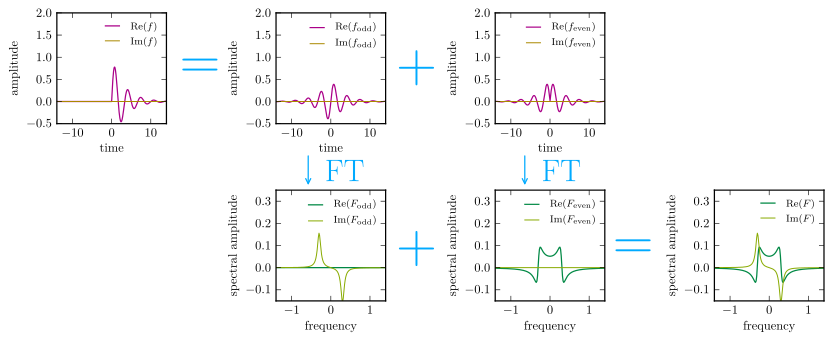
\includegraphics[width=17.5cm]{img/Kramers_Kronig_plot/kk.pdf}
\end{figure}
The Fourier transform of a real odd function is an imaginary function:
%F_{odd}(\omega)=& \int_{-\infty}^{\infty} e^{-\ii \omega t} f(t) \mbox{d}t = \\
		 %=&  \frac{1}{2} \int_{0}^{\infty} e^{-\ii \omega   t } [ f_{odd}(t) + f_{even}(t)] \mbox{d}t 
		   %+ \frac{1}{2} \int_{0}^{\infty} e^{-\ii \omega (-t)} [-f_{odd}(t) + f_{even}(t)] \mbox{d}t  \\
		 %=&  \int_{0}^{\infty} \frac{e^{-\ii \omega t}-e^{+\ii \omega t}}{2} f_{odd}(t) \mbox{d}t 
		   %+ \int_{0}^{\infty} \frac{e^{-\ii \omega t}-e^{+\ii \omega t}}{2} f_{odd}(t) \mbox{d}t  = \\
		 %=&\int_{-\infty}^{\infty} e^{-\ii \omega t} f(t) \mbox{d}t  = \\
		 %=&\int_{-\infty}^{\infty} e^{-\ii \omega t} f(t) \mbox{d}t  = \\
\begin{equation} 
\begin{split} 
F_{odd}(\omega)=& \int_{-\infty}^{+\infty} e^{-\ii \omega t} f_{odd}(t) \,\mbox{d}t = 
		 \int_{-\infty}^{+\infty} \frac{e^{-\ii \omega   t }}{2} f_{odd}(t) \,\mbox{d}t 
		   +  \int_{-\infty}^{+\infty} \frac{e^{-\ii \omega (-t)}}{2} [-f_{odd}(-t)] \,\mbox{d}t  \\
		 =&   \int_{-\infty}^{+\infty} \frac{e^{-\ii \omega t}-e^{+\ii \omega t}}{2} f_{odd}(t) \,\mbox{d}t 
		 = -\ii \underbrace{\int_{-\infty}^{+\infty} \sin(\omega t) \, f_{odd}(t) \,\mbox{d}t}_{\mbox{$\in \mathbb{R}$}},
\end{split} 
\label{eq_kkF}\end{equation}
whereas the Fourier transform of a real even function yields a real function:
\begin{equation} 
\begin{split} 
F_{even}(\omega)= \ldots =   \int_{-\infty}^{+\infty} \frac{e^{-\ii \omega t}+e^{+\ii \omega t}}{2} f_{even}(t) \,\mbox{d}t 
		 = \underbrace{\int_{-\infty}^{+\infty} \cos(\omega t) \, f_{even}(t) \,\mbox{d}t}_{\mbox{$\in \mathbb{R}$}}.
\end{split} 
%% TODO the following is WRONG! see ---->  http://www.thefouriertransform.com/pairs/step.php#signum,  ho3.pdf
\label{eq_kkFeven}\end{equation}
The odd and even components of the time-domain response function correspond to the imaginary and real part of the response spectrum, respectively:
\begin{equation} F_{odd}(\omega) + F_{even}(\omega) = F(\omega), \text{ where } F_{odd}(\omega) = F''(\omega) \text{ and } F_{even}(\omega) = F'(\omega).  \label{eq_kkFodd}\end{equation}
At the same time, $f_{even}(t)$ and $f_{odd}(t)$ are related to each other by having the opposite sign for $t<0$ and the same sign for $t>0$, that is 
\begin{equation} f_{even}(t) = \mbox{sign}(t)\,f_{odd}(t). \label{eq_kkfeven}\end{equation}
Multiplication in the time domain manifests as a convolution in frequency domain
\begin{equation} 
F_{even}(\omega) = \int_{-\infty}^{+\infty}  \frac{-2\ii}{\omega - \Omega} F_{odd}(\omega) \,\mbox{d}\Omega  \equiv  \left[\frac{-2\ii}{\omega}\right]\,\ast\,F_{odd}(\omega),
\label{eq_kkresult}\end{equation} 
where we used the knowledge that the $-2\ii/\omega$ function is the Fourier transform of $\mbox{sign}(t)$. Convolution with this function is also known as the Hilbert transform.% tODO cite

Obviously, Eq. (\ref{eq_kkfeven}) can also be converted to $f_{odd}(t) = \mbox{sign}(t)\,f_{even}(t)$, thus the relation between the real and imaginary part of the response spectrum also holds when $F_{odd}(\omega)$ and $F_{odd}(\omega)$ are exchanged in Eq. (\ref{eq_kkresult}). 

A related mathematical proof of Kramers-Kronig relations can be derived from the analyticity of the response function in the complex plane of frequency. %% TODO cite

%% TODO: why do K-K relations forbid to choose arbitrary phase difference over an unit cell? 
%% ie. Why the Neff can be unambiguously extracted from spectra?
% TODO show how it dictates the "constant area of imaginary part " when resonance Q is changed
%}}}

\subsection{Dispersion relations in local Drude-Lorentz media} \label{disp_rel_local_media}
\paragraph{Lower and upper polariton branches of transverse waves}  % TODO%{{{
Returning to the derivation of dispersion relations, we start with modifying the constitutive relation (\ref{eq_ce}) to a plane wave propagating in a medium:
\begin{equation}		\D := \varepsilon_0\epsrl(\omega)	\E, \quad\quad\quad						\B := \mu_0\mu_r(\omega)		\HH,				 \label{eq_ce2}\end{equation}
with the relative permittivity $\epsrl(\omega)$ and permeability $\mu_r(\omega)$ being two dimensionless functions of frequency, defined in Eq. (\ref{eq_lorentz_eps}, \ref{eq_lorentz_mu}). 
The wave equation (\ref{eq_wavek}) then changes to
\begin{equation}  T\E =  -\frac{\kk (\kk \cdot \E)}{k^2} + \E            = \varepsilon_0 \mu_0  \epsrl(\omega) \murl(\omega) \, \frac{ \omega^{2}}{k^2} \E.  \label{eq_wavek_disp}\end{equation}
which, in the isotropic case, results in the dispersion curve for the transverse electromagnetic wave 
\begin{equation} k(\omega) = \sqrt{\varepsilon_0 \mu_0} \sqrt{\epsrl(\omega) \mu_{r}(\omega)}\;\omega = \sqrt{\epsrl(\omega) \mu_{r}(\omega)}\; \frac{\omega}{c}, \label{eq_dispeq_loc}\end{equation}
with the added frequency-dispersive term responsible for the deviation of Fig. \ref{fg_dcsimpleel} from the original straight light line in Fig. \ref{fg_dcvac}. 





In the simplest example of a single electric resonance with negligible losses, as in Fig. \ref{fg_dcsimpleel}, the curve is divided into two separate branches. The \textit{lower polariton branch} is below the resonance frequency $\omega_0$ and is characterized by the Lorentz oscillator being in phase with the electric field. Above $\omega_0$, the dipoles of the Lorentz oscillator can no more follow the electric field and are opposite to it, thus the response of the medium is negative. With further increase of the frequency, the permittivity crosses zero at the frequency $\omega_{\text{L}}$. %, > \omega_0 which allows the transverse wave to propagate. 
where the \textit{upper polariton branch} starts. In case of a Lorentz oscillator unaffected by the presence of others, the difference $\omega_{\text{L}} - \omega_0$ can be computed from the magnitude of the oscillator (using the Lydanne-Sachs-Teller relation) \cite{klingshirn2007semiconductor}.

The same behaviour is observed for a single resonance in the permeability $\mu_r(\omega)$, and will be typical also for the spectra of resonances of macroscopic structures described later.

Note that the formation of upper and lower polariton branches can be reinterpreted\cite{landau1984electrodynamics} using the theory of coupled oscillators as the result of \textit{anticrossing} between the oscillator at the frequency $\omega_0$ (forming a horizontal line) and the photon branch (forming a straight growing light-line).

When losses are present, the lower and upper polariton branches are connected by a smooth line of \textit{anomalous} dispersion and very high losses.  % TODO \ref{fg_dispersion_polariton}
%}}}
\paragraph{Longitudinal waves in dispersive media} %{{{
The wave equation in local dispersive media (\ref{eq_wavek_disp}) 
%\begin{equation} - \kk (\kk \cdot \E) + k^2 \E = \varepsilon_0 \epsrl(\omega) \mu_0 \murl(\omega) \omega^{2} \E, \tag{\ref{eq_wavek_disp} \again} \end{equation}
also allows the existence of longitudinal waves with electric field parallel to the wave vector $\E || \kk$. It was shown earlier that there is no solution for longitudinal waves in vacuum except for a static homogeneous field.

\begin{figure}[t] \caption{Influence of a single resonance in the real part of relative permittivity $\epsrl'(\omega)$ (magenta curve in the left panel) to the shape of dispersion curves in the right panel (green curve, computed using Eq. (\ref{eq_dispeq_loc}). The lower and upper polariton branches are separated by a spectral region $\omega \in (0.3, 0.65)$, where the wave does not propagate on an appreciable distance (nonzero losses yield a finite solution here, though).} \label{fg_dcsimpleel} \centering  %% TODO refto
	\includegraphics[width=17cm]{img/dispersion_landau_lifshitz/dispersion_simple_el.pdf}
\end{figure}
If a local medium is assumed, and the wavenumber $k$ is nonzero, such waves can have a solution with nonzero $\E$ when $\epsrl(\omega)' = 0$, or with nonzero $\HH$ when $\mu_r(\omega)' = 0$. Therefore, the corresponding dispersion curve for a longitudinal wave is a horizontal line at $\omega = \omega_{\text{L}}$, independent of $k$. This would be equivalent to a standing oscillation that maintains the spatial amplitude envelope that was originally excited. 

Different physical phenomena can lead to $\epsrl(\omega)' = 0$, some of which introduce relatively low losses at the corresponding $\omega_{\text{L}}$; namely lattice vibrations in nonconductive crystals or electrons in inductive media (like metals and dilute plasma). 

At the interface of two media with negative and positive permittivity, another type of waves can be excited with an intermediate frequency $\omega < \omega_{\text{L}}$ that can not propagate in either of the bulk medium. The dispersion curve of such waves is not flat, allowing them to propagate along the interface. Depending on the mechanism, they are known as  \textit{surface plasmons} or \textit{surface phonon-polaritons} \cite[p. 87]{klingshirn2007semiconductor}, respectively. Accordingly, \textit{surface magnons} should be observed at interfaces where $\mu$ changes its sign.
% Are there surface magnons?
% Are there any metamaterials designed for longitudinal waves?
%}}}
\paragraph{Anisotropy of permittivity} \label{par_anisotropy} %{{{
It shall be noted here that permittivity $\epsrl$ was introduced as a scalar, assuming that the vector of electric field $\E$ and electric induction $\D$ are always of the same orientation:
\begin{equation} \D = \varepsilon_0 \epsrl(\omega) \E \equiv \varepsilon_0  
	\left(\begin{array}{ccc} 
			\epsrl(\omega) & 0 & 0  \\
			0 & \epsrl(\omega) & 0  \\
			0 & 0 &\epsrl(\omega)  
	\end{array} \right) \cdot \E
	\label{eq_}
\end{equation}
In some media of lower rotational symmetry (such as many crystals, or liquids under static electric field), the medium response depends on the electric field direction. At the beginning of the chapter, however, we assumed the fields are relatively weak, and we imposed the requirement of \textit{linearity} of the medium. Whatever the linear relation of $\D := \mathcal{L}(\E)$
is, it must obey the rule
$$\D_1 + \D_2 = \mathcal{L}(\E_1) + \mathcal{L}(\E_2) = \mathcal{L}(\E_1 + \E_2)$$
for any vectors $\E_1, \E_2$. Such a relation can be fully described by a \textit{tensor of permittivity} % TODO cite 
\begin{equation} \D = \varepsilon_0 \epsrl(\omega) \E \equiv \varepsilon_0  
	\left(\begin{array}{ccc} 
	{\epsrl}_{xx}(\omega) & {\epsrl}_{xy}(\omega) & {\epsrl}_{xz}(\omega)  \\
	{\epsrl}_{yx}(\omega) & {\epsrl}_{yy}(\omega) & {\epsrl}_{yz}(\omega)  \\
	{\epsrl}_{zx}(\omega) & {\epsrl}_{zy}(\omega) & {\epsrl}_{zz}(\omega)  
	\end{array} \right) \cdot \E.
	\label{eq_epstensor}
\end{equation}
Elaborate discussion on all possible forms of this tensor and their physical interpretation can be found e.g. in \cite[pp. 678--686]{born1999book}. An analogous treatment can be applied to the magnetic permeability, though it is less often needed.

%}}}
\paragraph{Dispersion relations in anisotropic local media}  %{{{
If the medium response depends on the direction of the field, the dispersion relations can not be directly obtained by substitution into the wave equation as in Eq. \ref{}. 

%\begin{equation} xxx  T\E :=  -\frac{\kk (\kk \cdot \E)}{k^2} + \E            = \frac{\mu_0 \varepsilon_0 \omega^{2}}{k^2} \E.  \label{eq_wavek}\end{equation}
%\begin{equation} xxx - \kk (\kk \cdot \E) + k^2 \E = \varepsilon_0 \epsrl(\omega) \mu_0 \murl(\omega) \omega^{2} \E,  \end{equation}

%is a linear transformation of the vector $\E$, which can be expressed by the tensor
%$$ - \kk (\kk \cdot \E) \equiv 
	%-\left(\begin{array}{c} k_x \\ k_y \\ k_z \end{array} \right) \cdot
	%\left[\left(\begin{array}{ccc} k_x & k_y & k_z \end{array} \right) \cdot
	%\left(\begin{array}{c} E_x \\ E_y \\ E_z \end{array} \right)\right] 
		%\equiv
	%\left(\begin{array}{ccc} -k_x^2 & -k_x k_y & -k_x k_z \\ -k_y k_x & -k_y^2 & -k_y k_z \\ -k_z k_x & -k_z k_y & -k_z^2 \end{array} \right) \cdot  
	%\left(\begin{array}{c} E_x \\ E_y \\ E_z \end{array} \right).
	%$$
%$$ k^2 \E \equiv 
%	\left[\left(\begin{array}{ccc} k_x & k_y & k_z \end{array} \right) \cdot 
%	\left(\begin{array}{c} k_x \\ k_y \\ k_z \end{array} \right)\right] \cdot 
%	\left(\begin{array}{c} E_x \\ E_y \\ E_z \end{array} \right),
%	$$
%$$ \mu_0 \varepsilon_0 \omega^{2} \E \equiv 
%	\left(\begin{array}{ccc} k_x^2+k_y^2+k_z^2 & 0 & 0 \\ 0 & k_x^2+k_y^2+k_z^2 & 0 \\ 0 & 0 & k_x^2+k_y^2+k_z^2 \end{array} \right) \cdot  
%	\left(\begin{array}{c} E_x \\ E_y \\ E_z \end{array} \right),
%	$$
The dispersion relation can however still be understood \cite[pp. 667]{born1999book} as a set of three linear algebraic equations:
\begin{equation}  T\E =  -\frac{\kk (\kk \cdot \E)}{k^2} + \E            = \frac{\varepsilon_0 \mu_0 \, \epsrl(\omega) \murl(\omega) \omega^{2}}{k^2} \E. \tag{\ref{eq_wavek_disp} \again}\end{equation}
%\begin{equation} \left|\begin{array}{ccc} 
	%k_y^2+k_z^2 - \mu_0 \varepsilon_0 \omega^{2} 		& -k_x k_y 		& -k_x k_z \\ 
	%-k_y k_x 		& k_x^2+k_z^2-\mu_0\varepsilon_0\omega^{2} 		& -k_y k_z \\ 
	%-k_z k_x 		& -k_z k_y		& k_x^2+k_y^2-\mu_0\varepsilon_0\omega^{2}
	%\end{array} \right| = 0, \label{eq_dispdet}\end{equation}
where the wave-plane projection tensor $T$, dependent on the wavevector $\kk$, was already defined in Eq. (\ref{eq_transverse}).

For simplicity, we assume here that the relative permeability $\murl = 1$; the extension to other cases is possible, too. %% TODO Do epsilon and mu commute, if they are both tensors??
A solution of Eq. \ref{eq_wavek} can exist with nonzero $\E$ if and only if the determinant of the set of three linear equations is zero:
\begin{equation} 
\det\left[
T -
	\frac{\mu_0 \varepsilon_0 \omega^2}{k^2}
	\left(\begin{array}{ccc} 
	{\epsrl}_{11}(\omega) & {\epsrl}_{21}(\omega) & {\epsrl}_{31}(\omega)  \\
	{\epsrl}_{12}(\omega) & {\epsrl}_{22}(\omega) & {\epsrl}_{32}(\omega)  \\
	{\epsrl}_{13}(\omega) & {\epsrl}_{23}(\omega) & {\epsrl}_{33}(\omega)  
	\end{array} \right) \right] = 0, \label{eq_dispdet}\end{equation}
The search for dispersion curves in an anisotropic medium is thus transformed into finding zeroes of this function of four scalar variables, $k_x$, $k_y$, $k_z$ and $\omega$.
In the most general case, it can be solved by means of numerical algebra software. 

\todo{verify}
For a given frequency $\omega$, rigorous solution of Eq. \ref{eq_dispdet} in local media gives in fact three solutions, of which two are for different polarisations of a transverse wave, and the third is for the longitudinal wave. The two transverse solutions give identical wave vector (are degenerate) if the medium is isotropic, or if $\kk$ points along the optical axis. 
% The longitudinal wave ... ?

%}}}
\paragraph{Isofrequency contours}  %{{{
%A resonance in local permittivity (or permeability) creates two polariton branches -- thus the dispersion curves can not be expressed as one simple function $\omega(k)$ of the wavevector $k$. It would then appear adequate to treat dispersion curves as a function of frequency, $k(\omega)$, but as is shown below in the presence of nonlocal response, neither $k$ is necessarily a simple function of $\omega$. Also 
It is often important to describe the dispersion curves also for different wave angles, which is the best accomplished by plotting the  %% todo ...real part of ...
frequency $\omega$ as the function of \textit{wave vector} $\kk$. In three dimensions, this would require mapping a function of three independent variables, $\omega(\kk) = \omega(k_x, k_y, k_z)$. However, in most cases the projection of two selected components of $\kk$ is sufficient to understand all relevant phenomena, and naturally it is much easier to visualize. 
\begin{figure}
  \begin{minipage}[c]{0.5\textwidth}
\hfill
    \includegraphics[width=7cm]{img/dispersion_curves_to_ifc.pdf}
  \end{minipage}
  \begin{minipage}[c]{0.5\textwidth}
    \caption{The relation between a plot of a dispersion curve for one photonic branch and the corresponding isofrequency contours. At a selected frequency, all points in the $k_x$-$k_y$ plane are drawn for which a nonzero solution of Maxwell equations exists. For transverse waves in local media, this is equivalent to finding a solution to the dispersion equation (\ref{eq_dispeq_loc}).\\Multiple frequencies can be plotted to describe the frequency dependence. For illustration, an isotropic medium was used, thus all IFCs take the form of a circle. To save space, only one quarter of the circle was plotted here.} \label{fg_ifc_dc}
  \end{minipage}
\end{figure}

Such a plot is known as \textit{isofrequency contours} (IFC), or also \textit{equifrequency contours} (EFC), and allows for intuitive geometrical analysis of various phenomena such as light refraction, beam walk-off, total internal reflection etc. 
The relation between a dispersion curve for one photonic branch and the corresponding isofrequency contours in an isotropic medium is shown in Fig. \ref{fg_ifc_dc}.

Its limitation is, however, that IFC plots do not show the imaginary part and thus are applicable to plot the dispersion in media with no or negligible losses only.  
Each photonic branch also has to be plotted in a separate plot to prevent the contours from overlapping (see the right panel of Fig. \ref{fg_dcsimpleel}). 
Moreover, in every single photonic branch, Eq. \ref{eq_dispdet} yields two solutions for two possible polarisations of transverse waves \cite[p. 46]{klingshirn2007semiconductor}. The IFCs for these solutions are generally different in anisotropic media, but we always restrict the discussion only one polarisation in the following figures  for simplicity. % \todo{discuss? In uniaxial media, where two diagonal components of the }

\begin{figure}[ht] \caption{An example of circular isofrequency contours, centered in the $k=0$ point, for a medium with isotropic permittivity \textbf{(a)}, with IFCs forming circles. 
 \textbf{(b)} The case of nondispersive anisotropic permittivity, forming elliptic IFC, and a similar case \textbf{(c)} with general orientation of the optical axis (drawn as dashed black line).
%% FIXME \textbf{(d)} A dispersive \textit{hyperbolic medium}, with one component being a function of frequency and crossing zero.
} \label{fg_ifc} \centering  %% TODO verify in Belov that local media may be used  as hyperbolic
	\includegraphics[width=.8\textwidth]{img/ifc_freqdispersion.pdf} 
\end{figure}
Isofrequency contours are valuable for graphical prediction of wave refraction on interface of two media \cite[p. 118]{shalaev2010book}. Starting, e.g., in the isotropic medium in Fig. \ref{fg_ifc}a, the wavevectors are known for given frequencies (as three coloured arrows).
The component of wave vector parallel to the interface (chosen as $k_x$ here and indicated by the vertical dashed lines) must be maintained upon refraction. This rule can be intuitively deduced from the continuity of the wave phase at the interface, as well as from the Noether theorem applied to the infinite translational symmetry of the interface. Transferring the vertical dashed lines to IFC plot of another medium and finding the intersections with an IFC of the corresponding frequency, one can find the new wavevector. 
In Fig. \ref{fg_ifc}, we provide examples of IFCs for one isotropic and two anisotropic media.

%}}}
\paragraph{Index of refraction and its applicability}  %{{{
With the background of the theory developed above, the notion of the \textit{index of refraction} $N$ can be properly introduced and discussed. 
In the most strict sense, the index of refraction is defined only for \textit{isotropic} media. Then it is equivalent to the ratio of the wavenumber $k(\omega) \equiv |\kk|$ to the wavenumber in vacuum at the same frequency: 
\begin{equation} N(\omega) := k(\omega) \, \frac{c}{\omega} \equiv \sqrt{\epsrl(\omega)\murl(\omega)}, \label{eq_}\end{equation}
as directly follows from Eq. (\ref{eq_dispeq_loc}).

Starting with a harmonic plane wave with the frequency $\omega$ and the wave vector $\kk^{(1)}$ refracting at an interface of two isotropic media, the projection of $\kk$ to the interface is given as 
$$ k_x = k^{(1)}\,\sin \alpha^{(1)}, $$
where $\alpha^{(1)}$ is the angle between the wavevector in the first medium $\kk^{(1)}$ and the  normal to the interface. In the second medium, a similar relation must apply, however the wavenumber $k^{(2)}$ may be different and as a result, the angle in the second medium is
\begin{equation} \alpha^{(2)} = \arcsin\left( \frac{k^{(1)}}{k^{(2)}} \,\sin \alpha^{(1)} \right) = \arcsin\left( \frac{N_1}{N_2} \,\sin \alpha^{(1)} \right), \label{eq_snell}\end{equation}
which is known as the \textit{Snell} (or also \textit{Snell-Descartes}) law.

The majority of (effective) media discussed in this thesis are however more or less anisotropic, and somewhat surprisingly, the notion of \textit{index of refraction} $N$ seems to be widely used for them in the literature anyway. The author thus feels there is a need for a conscientious extension of $N$ for anisotropic cases, too. An extremely loose definition of $N$ could be based on computing the ratio $N(\omega, \kk) := kc/\omega$  for any medium. This can be formally done, but then the wavenumber $k$ would also depend on the direction $\alpha$, and the Snell law in Eq. (\ref{eq_snell}) would become an implicit equation, losing its original purpose of making the computation explicit and notably simple.

The author proposes instead to restrict the term \textit{index of refraction} to all cases where IFCs are perpendicular to $\kk$. This covers not only all isotropic media, but also those cases when the waves propagate close the optical axis of any anisotropic media. An example of an anisotropic medium with its optical axis oriented in such a way that the refraction can be computed using Snell law provided the $k_x$ component is shared with \ref{fg_ifc}a, is shown in Fig. \ref{fg_ifc}c. For small deviations from this angle, where the IFC can be approximated by an osculating circle, 
\begin{equation} \frac{\partial k}{\partial \alpha} \ll k,\label{eq_osculating}\end{equation}
the Snell law still gives a correct prediction of the refraction angle. 

We will however show in the following that the prediction of \textit{beam} propagation is more complicated, being sensitive to the \textit{curvature of IFC}. 

%}}}
%%   \paragraph{Isofrequency contours of hyperbolic media}  %{{{ TODO READ BELOV2003 and FIXME
%%   The IFCs in Fig. \ref{fg_ifc}a,b,c were plotted for non-dispersive media, i. e. with $\epsrl$ and $\murl$ independent of frequency. The case of one polariton branch of a dispersive isotropic medium is already shown in Fig. \ref{fg_ifc_dc}, characteristic by non-equidistant IFCs which lead to the refraction angle being dependent on the frequency.
%%   
%%   A more complicated cases are the \textit{hyperbolic media}, where, in a certain spectral region, one component of the anisotropic permittivity is positive, while another one is negative. The solution of Eq. (\ref{eq_dispdet}) then results in a hyperboloid, which is either of one sheet or two sheets, depending on the sign of the remaining diagonal component of permittivity tensor. At the frequencies where the dispersive component of permittivity is negative,  
%%   Note that a negative permittivity is always connected with the dispersive behaviour, thus \ref{fg_ifc}d is another example of a dispersive medium. 
%%   
%%   %}}}
\paragraph{Phase velocity and group velocity}  %{{{  todo near single resonance
So far only the propagation and refraction of an infinite, single-frequency wave was discussed, and it was shown that it is determined by the shape of IFC at the given frequency. %% todo rewrite to more precise

If the wave is temporally modulated, its envelope in time is given as a complex vector function $\E_0(t)$ replacing the constant vector $\E_0$ in Eq. \ref{eq_pw}. This can be equivalently expressed in the frequency domain as the wave being formed by superposition of multiple frequency components, with respective amplitudes given by the Fourier transform of $\E_0(t)$. The position of the envelope in time is determined by their \textit{mutual phase difference}, not by the absolute wave phase. 

A similar argument can be made regarding the spatial modulation of the wave. Any wave shape other than the infinite plane wave is a superposition of waves with different wavevectors, and the direction of propagation of the spatial envelope is given by mutual phase difference of the constituent waves. % TODO rewrite-unclear

The velocity vector of the envelope propagation, denoted as the \textit{group velocity} $\mathbf{v_g}$, can be found as the gradient of frequency by the wavevector: %% TODO cite
\begin{equation} \mathbf{v_g} := \frac{\partial \omega}{\partial \kk} \equiv 
\left(\begin{array}{c} 
	\partial \omega/\partial k_x \\ 
	\partial \omega/\partial k_y \\ 
	\partial \omega/\partial k_z \\ 
	\end{array} \right)
 \label{eq_vg}\end{equation}
In the IFC plot, the group velocity can be visually found as directing always perpendicular to the IFC, with its magnitude being proportional to the density of the IFCs.

If the group velocity is different from the phase velocity, the envelope $\E_0(t)$ is maintained over time, but it continuously shifts against the underlying wave. Thus the actual temporal shape of $\E(t)$ changes upon passing through a dispersive medium.
On the contrary, in vacuum or media with negligible dispersion, each frequency component of the wave acquires an additional phase strictly proportional to its frequency. Then the group velocity coincides with the phase velocity: 
$$\hspace{3cm}\mathbf{v_g} = \kk \omega / k^2 \hspace{3cm} \text{(in nondispersive isotropic media)}.$$
%The orientation of $\vg$ and $\kk$ is usually the same, but later it will be shown that it can be otherwise, with peculiar physical consequences.

Usually in spectral regions near a resonance, also the quadratic or even higher terms in the Taylor expansion of the $\omega(\kk)$ dependence shall be taken into account. This effect is known as the \textit{group velocity dispersion} as it is equivalent to the group velocity $\vg(\kk)$ being dependent on the wavevector (or, if reformulated, on frequency). It results in temporal distortion of the wave envelope $\E_0(t)$.  %% TODO ... and what about distortion in space?
%}}}
\paragraph{Propagation of a beam in anisotropic media}  %{{{  
The refraction of a beam is illustrated in Fig. \ref{fg_ifc2} by means of three slightly different wavevectors it is composed of. For simplicity, a monochromatic wave was used, so brown, black and violet were chosen for the three example wavevectors to prevent confusion with the rainbow-like frequency color map used in Fig. \ref{fg_ifc}. 

In the first plot, \ref{fg_ifc2}a, the case of an isotropic medium is illustrated. Upon refraction into a general anisotropic medium in Fig. \ref{fg_ifc2}b, each component must maintain its wavevector projection to the interface, thus the wavevectors spread in their direction. The resulting beam propagates along the group velocity that is different from the central wavevector; % The components of the resulting beam are   is narrower and does not propagate 
this is also known as the spatial \textit{walk-off}.
\begin{figure}[ht] \caption{Examples of IFC similar to Fig. \ref{fg_ifc}, but with different wavevectors at a single frequency. \textbf{(a)} The wavevectors in the isotropic medium lie on a circle.
 \textbf{(b)} \textbf{(c)} } \label{fg_ifc2} \centering  %% TODO  WRITE
	\includegraphics[width=\textwidth]{img/ifc_kdispersion_hyp.pdf} 
\end{figure}


Fig. \ref{fg_ifc2}c shows again the special case of anisotropic medium, where the wave propagates near the optical axis, and thus where the Snell law can still be used to determine the refraction of a plane wave, based the generalized notion of the index of refraction.
However, there is a pitfall if one tries to apply the Snell law for prediction of how the beam will refract. The problem originates from the differential nature of the group velocity definition in Eq. (\ref{eq_vg}). 
%While the magnitude of the wavevector changes only negligibly, with the square of a 
While the phase velocity of a monochromatic wave at the frequency $\omega_0$ does not appreciably change upon a small deviation of the angle $\alpha$ from the optical axis  [c.f.  Eq. (\ref{eq_osculating})], the group velocity direction does, because it has a nonzero linear component in its dependence on the wavevector:
$$ \frac{\partial \vg(\kk)}{\partial \alpha} \neq 0.$$
As a result, the group velocity in anisotropic media is always much more sensitive to the angle than the phase velocity, and Snell law does not predict it correctly. It can be regarded as a spatially-dependent manifestation of the group velocity dispersion.

In Fig. \ref{fg_ifc2}d, an extreme case of spatial walk-off is shown on the example of a \textit{hyperbolic} medium with different signs of the permittivity along different axes. %% TODO study Belov2003 and possibly correct this if hyperbolas are wrong
 The normal to its IFC is nearly perpendicular to the wavevector, and accordingly, the beam refracts in opposite angle with regards to the incident wave. The $k_x$ component of the wave vector is however still maintained.

%If the amplitude and phase of the wave is not  temporal shape of a wave can be composed as a superposition of different frequency components with certain amplitude and phase. Similarly, any spatial shape of a beam can be composed of infinite waves of different wavevectors. The isofrequency contours, and their dependence on frequency, allow to determine how the temporal and spatial envelope will propagate. 
%Assuming a short pulse for simplicity

%}}}
\paragraph{The sign of the phase and group velocities}  %{{{
So far, in the discussion of refraction both in Fig. \ref{fg_ifc} and \ref{fg_ifc2}, the solution of the vertical wave vector component $k_y$ pointing downwards was always selected without providing justification. In fact, both upwards and downwards pointing wave vector provide valid solution. The reason is that in the first medium represented by the leftmost plots (Fig. \ref{fg_ifc}a and \ref{fg_ifc2}a), the incident wave was propagating downwards to the interface, and it was assumed that also the refracted wave will propagate downwards, from the interface.

A more complicated case occurs when the wave vector $\kk$ and group velocity $\vg$ point in opposite direction (or more generally, when they have an opposite projection on the normal to the interface).  This manifests as IFC radius \textit{decreasing} with frequency growing, as shown in  Fig. \ref{fg_ifcnr}.
Such a case can indeed occur in natural or artificial media, as described in more detail below. 
\begin{figure}[ht] \caption{Frequency-dependent IFCs of \textbf{(a)} an ordinary medium, \textbf{(b)} an isotropic medium with a negative index of refraction and \textbf{(c)} an anisotropic medium with a negative index of refraction \todo{comment}} \label{fg_ifcnr} \centering  %% TODO  WRITE
	\includegraphics[width=.8\textwidth]{img/ifc_negrefr.pdf} 
\end{figure}
\begin{figure}[ht] \caption{Wavevector-dependent IFCs for one frequency, for media choice the same as in Fig. \ref{fg_ifcnr} \todo{extend}} \label{fg_ifcnrk} \centering  %% TODO  WRITE
	\includegraphics[width=.8\textwidth]{img/ifc_negrefrk.pdf} 
\end{figure}

In the isotropic media, or the media where the wave vector points in direction close to the optical axis, the Snell law is still applicable, and we then speak of \textit{negative index of refraction}.  The refraction between an ordinary medium and two examples of negative-index media are plotted in Fig. \ref{fg_ifcnr}.
It should be noted that the negative-index media are necessarily dispersive. Therefore, the refraction of temporally short pulses disperses different frequencies into different angles, as can be found from the wavevectors at different frequencies in Fig. \ref{fg_ifcnr}b,c.

\todo{add that the propagation velocities are more complicated than this and will be discussed later; move a part of this text below?}
%}}}

\subsection{Nonlocal response} % TODO
\paragraph{Definition of nonlocal media}%{{{
%TODO: spatial dispersion describes one specific sort of nonlocal behaviour that exists in homogeneous infinite media only
The previous two chapters that concerned local media can be generalized into the theory of \textit{nonlocal} (or, \textit{spatially dispersive}) media that follows.

The downsides of the spatial-dispersive model of media is that it is more complicated, leading e.g. to an implicit dispersion equation. Its great advantage is however that it provides a necessary level of generality for the description of periodic structures discussed below. 
Some phenomena observed in the frequency spectrum are in fact consequences of the spatial dispersion, such as the Doppler broadening of resonance lines in gases \cite[p. 359]{landau1984electrodynamics}. More precisely, these phenomena are primarily dependent on the wave vector $\kk$, and their expression by means of the temporal spectrum is a mere approximation based on that the dispersion curve usually defines a simple relation between  frequency and wave vector.  %% TODO rewrite?

In this section such a more general class of media is discussed, where the medium response explicitly depends on the history of $\E(\tau, \brho)$ in previous time $\tau < t$ and in all surrounding points $\brho$, and therefore is described by a spatio-temporal convolution:
\begin{equation} \D(t,\rr) = \varepsilon_0 \E(t,\rr) + \varepsilon_0\int_{V} \int_{-\infty}^{t} \chi_e(t-\tau, \rr-\brho) \, \E(\tau,\brho) \,\mbox{d}\tau \,\mbox{d}^3\brho. \label{eq_chi_convol_nonloc}\end{equation}
In a very similar manner as in the local theory above, we assume a plane wave $\E(t, \rr) := \E_0 \, e^{\ii\omega t - \ii\kk\cdot\rr}$ propagates through the medium. This is without loss of generality, thanks to that it is possible to express any wave as a superposition of monochromatic plane waves.
\begin{equation} \D(t,\rr) = \varepsilon_0 \E_0 \, e^{\ii\omega t - \ii\kk\cdot\rr} + \varepsilon_0\int_{V} \int_{-\infty}^{t} \chi_e(t-\tau, \rr-\brho) \, \E_0 \, e^{\ii\omega \tau - \ii\kk\cdot\brho} \,\mbox{d}\tau \,\mbox{d}^3\brho. \label{eq_chi_convol_harm_nonloc}\end{equation}
After two  substitutions, $T:=t-\tau$, $\mathbf{R}:=\rr-\brho$, the exponent can again be separated into the original plane wave (which factors out), and a spatio-temporal Fourier transform of the medium response:
$$				 \D(t,\rr) = \varepsilon_0 \E_0 \, e^{\ii\omega t - \ii\kk\cdot\rr} + \varepsilon_0\int_{V} \int_{-\infty}^{0} \chi_e(T, \mathbf{R}) \, \E_0 \, e^{\ii\omega (t - T) - \ii\kk\cdot(\rr - \mathbf{R})} \,\mbox{d}T \,\mbox{d}^3\brho,$$
$$				 \D(t,\rr) = \varepsilon_0 \E_0 \, e^{\ii\omega t - \ii\kk\cdot\rr} + \varepsilon_0\left( \int_{V} \int_{-\infty}^{0} \chi_e(T, \mathbf{R})  \, e^{-\ii\omega T + \ii\kk\cdot \mathbf{R}}\,\mbox{d}T \,\mbox{d}^3 \mathbf{R} \right) \E_0 \, e^{\ii\omega t - \ii\kk\cdot\rr}.$$
The response of the medium to the electric field of any harmonic plane wave can now be expressed as a function of frequency $\omega$ and wave vector $\kk$. It is defined as the ratio between the electric displacement and the electric field:
\begin{equation} \epsrn(\omega, \kk) = \left.\frac{\D(t,\rr)}{\varepsilon_0 \E(t,\rr)} \right|_{\E(t, \rr) := \E_0 \, e^{\ii\omega t - \ii\kk\cdot\rr}}  = 1 + \int_{V} \int_{-\infty}^{0} \chi_e(T, \mathbf{R}) \,e^{-\ii\omega T + \ii\kk\cdot \mathbf{R}} \,\mbox{d}T \,\mbox{d}^3\mathbf{R} \label{eq_eps_nonloc}\end{equation}
Converting the problem from the spatio-temporal domain into the wavenumber-frequency domain allows to express the relation between $\D$ and $\E$ by the \textit{permittivity} function $\epsrn(\omega, \kk)$ and completely avoid the convolution from Eq. (\ref{eq_chi_convol_harm_nonloc}). Note that both the response function $\chi_e$ and the permittivity $\epsrn$ %% TODO make it \varepsilon_r
may be either scalar functions, or rank-2 tensor functions; the latter case accounts for possible anisotropy of the medium.
% , and convolution in space is equivalent to multiplication  in the reciprocal space

The terms of \textit{nonlocality} and of \textit{spatial dispersion} are used interchangeably in the literature. The difference seems to be related to the way one thinks about the medium -- while \textit{nonlocality} is obviously related to the description in the real space [cf. Eq. (\ref{eq_chi_convol_nonloc})], \textit{spatial dispersion} derives from that the response is not a constant function in the reciprocal $\kk$-space. In the author's view, the term \textit{spatial dispersion} is therefore of slightly narrower meaning, as it implies that a plane wave of a defined wavevector is considered in an infinite medium.

%}}}
\paragraph{Power expansion of the medium parameters} %{{{
Assuming the dependence of the medium permittivity $\epsrn(\omega,\kk)$ or permeability $\murn(\omega,\kk)$ is a function varying slowly with $\kk$, we can express them in general as power series \cite[p. 367]{landau1984electrodynamics}:
\begin{equation} 
\left.  \begin{array}{c}
\epsrn(\omega,\kk) = 1 + \chi_e(\omega) + \ii \gamma_{\text{e}}(\omega) \kk + [\alpha_{\text{e}}(\omega) \kk] \kk + \ldots, \medskip  \\
\murn(\omega,\kk) = 1 + \chi_m(\omega) + \ii \gamma_{\text{m}}(\omega) \kk + [\alpha_{\text{m}}(\omega) \kk] \kk + \ldots, 
\end{array} \quad \right\} \quad \text{(in any media)}
\label{eq_epsmusd1}\end{equation}
where $\chi_{e,m}(\omega)$ are tensors of the second rank, $\gamma_{e,m}(\omega)$ of the third rank, $\alpha_{e,m}(\omega)$ of the fourth rank, and similarly for possible higher orders of expansion. After the corresponding number of matrix multiplication with $\kk$, they all yield rank-2 tensors that add up to form the tensor of permittivity or permeability.
%In this customary symmetric approximation of local media, both the electric permittivity and permeability in Eq. (\ref{eq_eps_loc}) are composed of two terms, one caused by the immediate response of vacuum, and another by the response of matter. In nonlocal media, both functions depend on the wavevector $\kk$, making the solution of Maxwell equations more complicated.

Note the response function for a local medium can be formally derived from its nonlocal formulation by replacing the spatial dependence by a Dirac delta function: %% TODO fix the sencence - it is in fact incorrect
\begin{equation} \chi_e(t-\tau, \rr-\brho) = \delta^{3}(\rr-\brho) \; \chi_e(t-\tau), \label{eq_loc_chi}\end{equation}
which allows to simplify Eq. (\ref{eq_chi_convol_nonloc}) so that in local media only the temporal convolution has to be computed. Then the higher order terms including $\gamma_{e,m}$ and $\alpha_{e,m}$ in Eqs. (\ref{eq_epsmusd1}) vanish:
\begin{equation} 
\left.  \begin{array}{c}
\epsrn(\omega,\kk) = 1 + \chi_e(\omega) = \epsrl(\omega), \medskip \\
\murn(\omega,\kk) = 1 + \chi_m(\omega) = \murl(\omega). 
\end{array} \quad \right\} \quad \text{(in local media)}
\label{eq_epsmusd2}\end{equation}

%}}}
\paragraph{Magnetic effects can be described by nonlocal permittivity} %{{{
Here, we will follow the approach of Landau and Lifshitz (see \cite{landau1984electrodynamics}, and also \cite{krowne2007book_agran, agranovich2006spatial}) to show that the magnetic response of any medium can be fully expressed by a certain form of permittivity dependence on $\kk$. This leads to introducing new \textit{Landau-Lifshitz} permittivity and permittivity, which are, in general, different from those used in the more customary symmetric model:
$$\epsLL(\omega, \kk) \not\equiv \epsrn(\omega, \kk),\quad\quad\quad 1 = \muLL(\omega, \kk) \not\equiv \murn(\omega, \kk).$$
The Maxwell equations (\ref{eq_me1}-\ref{eq_me4}) however still hold when these new parameters are substituted for the original ones.
The advantage is that the relative magnetic permeability is defined as a mere constant of the magnetic response of vacuum $\muLL(\omega, \kk) := 1$, thus reducing the complexity of the computation compared to the symmetric spatial-dispersive model. %% [as in Eq. (\ref{eq_ce})]

%}}}
\paragraph{Local medium in the Landau-Lifshitz model} %{{{
For simplicity we assume %% ... or "start with" TODO extend also to nonlocal ones
the medium is local, and described by $\epsrl(\omega)$ and $\murl(\omega)$.
The new spatial-dispersive permittivity $\epsLL(\omega, \kk)$ then consists of the 
\begin{enumerate}
 \item{the component caused by the local electric response of matter,} 
 \item{a new component fully accounting for the \textit{magnetic} response of matter, thanks to a particular shape of its spatial dispersion.}
\end{enumerate}
This model may be easily extended later to accept nonlocal constitutive parameters.

Repeating the Maxwell equation (\ref{eq_me4}) that links the magnetic field $\HH$ with the electric induction $\D$, 
\begin{equation} \nabla \times \HH =  \frac{\partial \D} {\partial t}, \tag{\ref{eq_me4} \again} \end{equation}
it is clear that if one defines new pair of vector fields
\begin{equation} \HHsd = \HH + \frac{\partial\mathbf{X}}{\partial t}, \label{eq_HHsd}\end{equation}
\begin{equation} \Dsd  = \D  + \nabla\times \mathbf{X}, \label{eq_Dsd}\end{equation}
then Eq. (\ref{eq_me4}) maintains exactly the same form with the new fields, for any differentiable vector field $\mathbf{X}$:
\begin{equation} \nabla \times \HHsd = \nabla \times \HH + \left(\nabla\times \frac{\partial\mathbf{X}}{\partial t}\right) = \frac{\partial \D}{\partial t}+ \frac{\partial(\nabla\times \mathbf{X})}{\partial t} =  \frac{\partial \Dsd} {\partial t}, \label{eq_me4sd} \end{equation}
because for well behaved functions the temporal and spatial derivatives commute.

%% TODO how this transform is denoted?
With the freedom of choice of $\mathbf{X}$, we impose the above mentioned requirement that whole magnetic response of the matter is expressed by the constitutive equation for permittivity. Therefore in spatial-dispersive theory, the constitutive equation %% TODO reference some text from above pargraphs
for magnetic induction is defined the same as in vacuum:
\begin{equation} \mu_0 \HHsd := \mu_0 \murl(\omega) \HH = \B. \label{eq_mu_sd}\end{equation}
When this equation is rearranged into the form similar to \ref{eq_HHsd}, we obtain a prescription for sought $\mathbf{X}$: 
$$ \HHsd = \HH + (\murl(\omega) -1)\HH = \HH + \underbrace{\left(\frac{\murl(\omega)-1}{\mu_0\murl(\omega)}\right)\B}_{=:\,\partial\mathbf{X}/\partial t}$$
Without loss of generality, we again restrict the discussion to a plane wave (\ref{eq_pw}), thus the time derivative equals to multiplication by $\ii\omega$.
\begin{equation} \mathbf{X} = \frac{1}{\ii\omega}\left(\frac{\murl(\omega)-1}{\mu_0\murl(\omega)}\right)\B = \frac{1}{\ii\omega\mu_0}\left(1 - \frac{1}{\murl(\omega)}\right)\B. \label{eq_Xsd}\end{equation}
The new \textit{Landau-Lifshitz} electric displacement $\Dsd$ that also accounts for magnetic phenomena is obtained by substitution of Eq. (\ref{eq_Xsd}) into Eq. (\ref{eq_Dsd}):
\begin{equation} \Dsd := \D - \ii\kk\times \mathbf{X} =  \D - \ii  \frac{1}{\ii\omega\mu_0}\left(1 - \frac{1}{\murl(\omega)}\right) \kk\times \B  \label{eq_Dsd2}\end{equation}
By means of the other Maxwell equation (\ref{eq_me3}), the magnetic induction $\B$ can be substituted by $\kk\times\E / \omega$ to obtain an expression that contains the electric quantities only.
\begin{equation} \Dsd = \D - \frac{1}{\omega^2 \mu_0}\left(1 - \frac{1}{\murl(\omega)}\right) \kk\times(\kk\times \E).  \label{eq_Dsd3}\end{equation} 
Double vector multiplication on the right hand side can be identified with the wave-plane projection tensor $T$, c.f. Eqs. (\ref{eq_rotrot}, \ref{eq_transverse}):
\begin{equation} \Dsd = \D + \frac{k^2}{\omega^2 \mu_0}\left(1 - \frac{1}{\murl(\omega)}\right) \, T \E,  \label{eq_Dsd3}\end{equation} 

%}}}
\paragraph{Tensor form of the Landau-Lifshitz permittivity of local isotropic media}%{{{
%Continuing in the derivation outlined in , 
From Eq. (\ref{eq_Dsd3}) we can derive the tensor form of spatial-dispersive permittivity $\epsLL(\omega,\kk)$:
\begin{equation} 
\left.  \begin{array}{c}
\epsLL(\omega,\kk) = 1 \,+\, \chi_e(\omega) \;\;+\;\; \frac{k^2}{\omega^2 \mu_0}\left(1 - \frac{1}{\murl(\omega)}\right) \, T, \medskip \\
\muLL(\omega,\kk) = 1, 
\end{array} \quad \right\} \quad \text{(in local media)}
\label{eq_epsmusd3} \end{equation} 
where 
\begin{equation} T = \frac{1}{k^2} 
\left(\begin{array}{ccc} 
	k_y^2+k_z^2		& -k_x k_y		& -k_x k_z \\ 
	-k_y k_x		& k_x^2+k_z^2	& -k_y k_z \\ 
	-k_z k_x		& -k_z k_y		& k_x^2+k_y^2
	\end{array} \right) 
\text{ or equivalently, }
T_{ij} = - \frac{k_i k_j}{k^2} + \delta_{ij} . \tag{\ref{eq_transverse} \again} \end{equation}

Let us note that the classical approach using symmetric parameters $\epsrl(\omega,\kk),\murl(\omega,\kk)$, and the Landau-Lifshitz approach of gathering all medium-related effects in the permittivity $\epsLL(\omega,\kk)$ are only two examples of all possible transformations of medium parameters that keep the Maxwell equations unchanged. If needed, it is formally possible to use any other arrangement, which may moreover be frequency dependent, leading to a physically realistic pair of parameters with uncommon properties \cite{skaar2014}.

%% TODO REF EBD theory and nonlocal electrodynamics
%% \cite{krowne2007book_agran}
%% \cite{landau1984electrodynamics}
%% \cite{agranovich2006spatial}
%% \cite{mikki2009electromagnetic}
%% \cite{vinogradov2002form}
%% \cite{golubkov1995boundary}
%% \cite{agranovich2004linear}
%% \cite{agranovich1962crystal}
%}}}

\subsection{Dispersion relations in homogeneous nonlocal media} 
\paragraph{How a local dielectric manifests in the Landau-Lifshitz model} %{{{
\begin{figure}[th] \caption{Dispersion curves for three different examples of local mediua, comparing the symmetric and Landau-Lifshitz representation of constitutive parameters.\\
Left column: Local parameters $\epsrl(\omega)$, $\murl(\omega)$ as functions of frequency.\\
Right column: Dispersion curves were computed using Eq. (\ref{eq_disp}), either with the local parameters from Eq. (\ref{eq_epsmusd2}) [plot as green lines] or with the Landau-Lifshitz parameters from Eq. (\ref{eq_epsmusd3}) [plot as black contour]. The Landau-Lifshitz permittivity $\epsLL(\omega,\kk)$ is color shaded on the background.
} \label{fg_dcll} \centering  
	\includegraphics[width=1\textwidth]{img/dispersion_landau_lifshitz/dispersion_ll_el.pdf}
	\includegraphics[width=1\textwidth]{img/dispersion_landau_lifshitz/dispersion_ll_mag.pdf}
	\includegraphics[width=1\textwidth]{img/dispersion_landau_lifshitz/dispersion_ll_elmag.pdf}
\end{figure}

Both the dispersion curves and the isofrequency contours predicted by the classical and Landau-Lifshitz representations of the constitutive parameters should be identical. This is illustrated by Fig. \ref{fg_dcll} on three examples - of a medium with electric resonance, a magnetic resonance and both resonances overlapping. The left column shows the \textit{local} permittivity $\epsrl(\omega)$ and permeability $\murl(\omega)$.

The right column additionally shows the Landau-Lifshitz permittivity $\epsLL(\omega, k)$ as a colour map with blue tone for negative values and red for positive ones. The thin black line overlay connects all points where the dispersion equation holds. %% , $\epsLL(\omega, k) \,\omega^2 / k^2 = 1$. TODO this is more complicated, as epsLL is a tensor - find which equation to refer to
As a confirmation of the compatibility of the Landau-Lifshitz model with the classical one, the original green dispersion curve from Fig. \ref{fg_dcsimpleel} is retained, which was computed using the classical approach based on the Eq. (\ref{eq_dispeq_loc}). It can thus be seen that both models always predict exactly the same dispersion.

For a local isotropic medium with a single electric resonance in Fig. \ref{fg_dcll}a, the curves plotted are identical to Fig. \ref{fg_dcsimpleel}. The Landau-Lifshitz permittivity $\epsLL(\omega, k)$ follows a resonance curve in frequency, but is independent of the wavenumber $k$ (as long as the medium is local). With frequency increasing, the lower polariton branch bends towards higher $k$, as $\epsLL(\omega, k)$ increases towards the resonance at $\omega_0$, then a band of frequency follows where and no solution of the wave equation %% TODO REF
exists due to $\epsLL(\omega, k)$ being negative, and finally the upper polariton branch starts when $\epsLL(\omega, k)$ crosses zero and becomes positive again.

A local medium with a single \textit{magnetic} resonance, Fig. \ref{fg_dcll}b, is predicted by the symmetric model to exhibit a similar dispersion curves. At the right panel of Fig. \ref{fg_dcll}b, the magnetic resonance is represented by the
%%% TODO add Eq. 2.52 repeated with underbrace
contribution that grows proportionally with $k^2$, and its maximum magnitude is located at the frequency $\omega_{mp}$ where $\murl(\omega_{mp}) = 0$. This shape of $\epsLL(\omega, k)$ causes the lower polariton branch to bend and approach a horizontal asymptote, which is again separated by a band of no allowed wave from the upper polariton branch, starting at $\omega_{mp}$.
$\epsLL(\omega, k)$

Finally, in Fig. \ref{fg_dcll}c, both resonances are combined. The main difference from Fig. \ref{fg_dcll}a occurs in the frequency range where originally $\epsLL(\omega, k) < 0$ and no wave could propagate. However, the magnetic resonance increases $\epsLL(\omega, k)$ by a term proportional to $k^2$, and consequently a new photonic branch is formed with $\mathrm{d}\omega/\mathrm{d}k < 0$, that is, with opposite group and phase velocities. Thus, the medium behaves as described in Figs. \ref{fg_ifcnr}b and \ref{fg_ifcnrk}b.
 %The left panel of Fig. \ref{fg_dcll}a is therefore identical to the previous one. Its left panel is identical to that shown in Fig. \ref{fg_dcsimpleel}, as the medium can still be fully described by 
\pagebreak

 %(electric quadrupoles..., [Merlin])

%}}}
\paragraph{Why magnetic resonances do not contribute to static permeability?}%{{{
%}}}
\paragraph{Multiple waves at one frequency and additional boundary conditions}%{{{
%}}}

\subsection{Impedance and amplitudes of the refraction and reflection}
\paragraph{The interface of two local media}\todo{connect somehow with the rest of theory?} %{{{ 
So far, only the phase-related phenomena were discussed: based on the local or nonlocal response of the medium, the dependence of the dispersion curves and IFCs was computed. Geometrical arguments then were used to infer the angle of refraction at the interface of two media, showing e.g. that a positive or negative refraction may occur, that the beam may refract in different direction than the wave vector, and that in some cases the notion of index of refraction can be used to simplify the problem based on the Snell law.

The conservation of wave phase at the interface is, however, not the only constraint to the refraction/reflection problem: Assuming the surface current and surface charge are zero and that the  medium is local, the \textit{parallel} component of the fields $\E$, $\HH$ with regards to the interface must be continuous. Additionally, the \textit{perpendicular} component of the displacements, $\D$ and $\B$, is continuous, too. This can be deduced from the integral formulation of Maxwell equations [Eq.  (\ref{eq_me1}--\ref{eq_me4})], 

The reflection and refraction (i.e. transmission) coefficients are derived in many textbooks \cite[p. 38]{born1999book} with different levels of generalisation. In the particular case where wave perpendicularly impinging an interface of two isotropic local media, described by their impedances $Z_1, Z_2$, respectively, the (complex) reflection $r$ and transmission $t$ are
\begin{equation} r = \frac{Z_2 - Z_1}{Z_2+Z_1}, \quad t = \frac{2 Z_2}{Z_2 + Z_1}, \label{eq_reflection}\end{equation}
with the impedances
$Z_{12} = \sqrt{\frac{{\murl}_{12}}{{\epsrl}_{12}}}$.
\add{This is in fact similar to the reflection on a one-dimensional transmission line, as known from microwave engineering.}

If the incidence is not perpendicular, the complex amplitudes of the reflected and transmitted wave depend on the angle of incidence, and splits into the TE and TM polarisation.\todo{cite}

%}}}
\paragraph{Refraction between nonlocal media}\todo{has ever been discussed or computed?}   %{{{ TODO
The expansion of the impedance to spatial-dispersive media is, to the knowledge of the author, never done.\todo{...verify} The reason lies in the spatial-dispersive media always being assumed infinite, so their interfaces are not accounted for in the model. If such an extension would be done, the spatial integral in Eq. \ref{eq_eq_chi_convol_nonloc} would have to be better specified, either with the nonlocal response of medium to extend also behind the interface. Alternatively, the medium response could be sharply truncated at the interface.

%}}}

\subsection{Phase, group, energy and signal velocity in nonlocal media}
\paragraph{Sign of the phase and group velocities}%{{{ TODO
The negative refraction in media shown in Figs. \ref{fg_ifcnr}b,c and \ref{fg_ifcnrk}b,c was a result of the requirement for the group velocity $\vg$ to maintain its component perpendicular to the interface, and for the wave vector $\kk$ to maintain its projection onto the plane of interface. Therefore, in media with low losses, the term of negative refraction 
\add{... in media with time reversal, the wave may always propagate backwards - we should always speak of mutual sign of the velocities}
%}}}
\paragraph{"Negative-refraction", "negative-index", or "doubly-negative" media?}  %{{{
Media with a negative index of refraction are a subset of negative refraction, where the notion of index of refraction makes sense, as discussed above. }

\add{When the index of refraction $N = \sqrt{\epsrl\murl}$ and the impedance $Z = \sqrt{\frac{\murl}{\epsrl}}$ are both defined, one may easily deduce that 
\begin{equation} \epsrl = \pm\frac{N}{Z}, \quad \murl = \pm N\,Z. \label{eq_nzepsmu}\end{equation}
The question of indefinite sign can be decided using the assumption of medium \textit{passivity}, that is, of the medium absorbing the wave rather than amplifying it. \todo{describe further}

\todo{ (here first cite Veselago, not earlier, not later, note that Veselago68 speaks about a truly *homogeneous* medium)\\ }

\todo{add the comments from http://www.wave-scattering.com/negative.html}
}
%}}}
\paragraph{Sign of the group and energy velocities}  % TODO %{{{
\mdf{
% TODO 0401 how can one tell apart negative refraction due to eps-mu and due to higher, purely nonlocal terms?

*doubly resonant local media -> negative phase velocity, positive group velocity, above resonant frequencies - theoretically arbitrarily small losses\\
*singly resonant local media -> positive phase velocity, negative group velocity, this happens near resonance so there are always high losses\\
*			  nonlocal media -> weird things happen, todo\\

the group velocity can also be negative \cite{mcdonald2000negative, dolling2006simultaneous} or superluminal, but only in lossy media and under strong GVD\\

TODO FIGURE: a) eps resonant, mu constant     b) N positive, but group velocity dropping


Group velocity in lossy local media can be opposite to S

Poynting vector usually coincides with the group velocity -- or always?\\

phase velocity is often higher than the speed of light, this is no problem\\

\cite{Mikki}, group velocity can be negative or superluminal - no problem here?
}

%}}}
\paragraph{Signal velocity}%{{{
The notion of \textit{signal propagation velocity} is sometimes % TODO cite
used 

is a problematic term, because a finite-support function spans over infinite spectrum, where group velocity has to change and differ \\

Near a single resonance with damping, the phase velocity can drop \\

\mdf{
TODO FIGURE to show this?: a) eps resonant, mu constant     b) N positive, but group velocity negative\\

this happens only in the presence of a high absorption \cite{mikki2009electromagnetic}\\
}

%}}}
%% TODO \paragraph{Speed of light and causality in spatial-dispersive media}%{{{
%% \mdf{TODO REF Kramers-Kronig relations in nonlocal medium
%% \cite{skettrup1970kramers}
%% \cite{kirzhnitz1976}
%% \cite{melrose1977generalised}
%% \cite{sun1989kramers}
%% \cite{rozanov2003}
%% \cite{bruleanalysis}
%% \cite{makarov2013kramers}
%% }%}}}
%% 

\section{Electromagnetic waves in periodic structures}
\subsection{Bloch theorem}
%In a given time the wave in a periodic medium takes on the form of Bloch wave (\ref{eq_bloch}): 
 %$\mathbf{E}(\mathbf{r}) = \mathrm{e}^{\mathrm{i}Kz} \cdot \mathbf{u}(\mathbf{r})$, i.e. it is a product of a harmonic \textit{envelope} and a cell-periodic \textit{mode}. Computing the dispersion curves involves computing the envelope wavenumber $K = K(f)$ for each frequency $f$ in the desired spectrum. The information about the mode $\mathbf{u}(\mathbf{r})$ is not used and instead the metamaterial cell is treated as if it was a homogeneous medium -- therefore this procedure is also called \textit{homogenisation}.

\paragraph{The Bloch-Floquet theorem}%{{{
% TODO define periodicity

The important Bloch-Floquet theorem states that while the wave in periodic medium does not have to be periodic anymore, it is a product of two periodic functions:
\begin{equation} \E(t, \rr) = \mathrm{e}^{\mathrm{i} Kz - 2\pi \mathrm{i} f t} \cdot \mathbf{u}(\rr), \text{ where } \mathbf{u}(\rr) = \mathbf{u}(\rr+a\mathbf{z}) = \mathbf{u}(\rr+2a\mathbf{z}) = \ldots, \label{eq_bloch}\end{equation} 
The $\mathbf{u}(\rr)$ function has the same periodicity as the structure. It is generally a complex vector function so it not only alters the direction and magnitude of $\E$ (or  $\HH$), but can also introduce a \textit{phase modulation} of the wave in each unit cell. Note that the capital $\KK$ is used to distinguish the wave vector of the Bloch wave envelope from the wave vector $\kk$ in free space. Note this theorem does not determine how the shape of $\mathbf{u}(\rr)$ nor the direction and magnitude of $\KK$, it only states they do exist.
% TODO proof /home/filip/PhD/Sources_MM_theory/Bloch_Theorem_Proof.pdf
% TODO example illustration of Bloch wave -> plotted in Python

%}}}


\paragraph{Virtual periodicity and ambiguity of the mode function}%{{{
\add{
The simplest "structure" to be started with is surely the empty vacuum with homogeneous $\varepsilon := 1$ and $\mu := 1$. One particularly simple solution of the Maxwell equations in vacuum is the planar wave propagating along the $z$-axis, defined by Eq. (\ref{eq_pw2}).
Let us now introduce virtual periodicity, requiring that the vacuum properties are invariant under discrete translation by an arbitrary length $a$ along the $z$-axis, which naturally holds. The important Bloch-Floquet theorem states that while the wave in periodic medium does not have to be periodic anymore, it is a product of two periodic functions:

In a homogeneous medium, there is a simple \textit{dispersion} relation between the frequency  $f$ and the wavenumber $k$, given as
\begin{equation} f = \frac{ck}{2\pi \cdot n} = \frac{ck}{2\pi \cdot \sqrt{\varepsilon \mu}}. \label{eq_dispersionold}\end{equation}
The constant $n = \sqrt{\varepsilon \mu}$ connecting the frequency and wavenumber is the index of refraction.

\begin{figure}[ht] \caption{Folded and unfolded dispersion curves for free space and photonic crystal. The phase difference over an unit cell can be expressed either by the wavenumber $K$ (unfolded plots \textbf{a, b} above), or it can be partially absorbed into the periodic mode function $\mathbf{u}(\rr)$ (folded plots \textbf{c, d} below) } \label{fg_phc} \centering  %% TODO write caption; complement the text to match
	\includegraphics[width=17cm]{img/PhC_folding_illustration.pdf} 
\end{figure}
When the wavelength is less than double cell spacing, or equivalently when $2\pi c /K < 2 a$, the unit cells can scatter the forward propagating wave into the backward direction and vice versa. In an infinite periodic structure the energy transfer must be conserved, so the forward and backward waves must be of the same amplitude. (The equilibrium of forward and backward wave amplitudes may, however, differ in some cases even in in infinite periodic structure. One example is when the constituent materials lose time-reversal symmetry due to static magnetic field.) We assume this also in this example with virtual periodicity. The \textit{Bloch wave} (\ref{eq_bloch}) is a product of two functions, and it gives one degree of freedom to select which part of (\ref{eq_bloch}) expresses the phase shift across one unit cell. Two different conventions are used in the literature.
\begin{enumerate}
 \item{In the \textit{unfolded} plot, the phase shift is expressed entirely by the envelope $\mathrm{e}^{\mathrm{i}Kz}$. One can always find a line coming from the front side of a unit cell to its back side, along which the mode function does not change its phase significantly $\mathbf{u(\mathbf{r})}$. In other words, the volume of the unit cell is not divided by any \textit{nodal plane} in the real part of electric field  $\mathbf{u(\mathbf{r})}$. (However, closed nodal planes within the unit cell may appear due to individual resonances.)

In vacuum, the mode function takes the simplest form, being constant $\mathbf{u(\mathbf{r})} = 1$ at all frequencies. The dispersion relation of vacuum forms a direct line as plot in Fig. \ref{fg_phc}a.} 
 \item{The \textit{folded} plot requires $K/\left(\frac{2\pi}{a}\right) \in (-\frac{1}{2}, \frac{1}{2})$ and the remaining phase is mostly expressed by the mode function. 
Further savings of space in the plot can be made using the symmetry of the forward and backward waves, so only the positive half for $K/\left(\frac{2\pi}{a}\right) \in (0, \frac{1}{2})$ has to be plot to describe the mode structure.} 
 \end{enumerate}
Although maybe less instructive, usually the \textit{folded} bands are plot in the literature and they are used also in Fig. \ref{fg_1dbd}, \ref{fg_rodh} and \ref{fg_erod_radius11} below. The same approach can be used for periodic structures, where the bands are separated by band gaps, cf. Fig. \ref{fg_phc}b and \ref{fg_phc}d.
}
%}}}
\paragraph{Dispersion curves under virtual periodicity} \label{par_disp_curv_per}%{{{
The vacuum properties are obviously invariant under discrete translation by an arbitrary length $a$ along the $z$-axis, which can be considered a \textit{virtual} periodicity. 
% TODO mention the terminology "band diagram" - "dispersion curves", is there any real difference?

When the wavelength is less than double cell spacing, or equivalently when $2\pi c /K < 2 a$, the unit cells can scatter the forward propagating wave into the backward direction and vice versa. In an infinite periodic structure the energy transfer must be conserved, so the forward and backward waves must be of the same amplitude.\footnote{The equilibrium forward and backward wave amplitudes may, however, differ in some cases even in in infinite periodic structure. One example is when the constituent materials lose time-reversal symmetry due to static magnetic field.} We assume this also in this example with virtual periodicity. The \textit{Bloch wave} (\ref{eq_bloch}) is a product of two functions, and it gives one degree of freedom to select which part of (\ref{eq_bloch}) expresses the phase shift across one unit cell. Two different conventions are used in the literature.
\begin{enumerate}
 \item{In the \textit{unfolded} plot, the phase shift is expressed entirely by the envelope $\mathrm{e}^{\mathrm{i}Kz}$. One can always find a line coming from the front side of a unit cell to its back side, along which the mode function does not change its phase significantly $\mathbf{u(\rr)}$. In other words, the volume of the unit cell is not divided by any \textit{nodal plane} in the real part of electric field  $\mathbf{u(\rr)}$. (However, closed nodal planes within the unit cell may appear due to individual resonances.)

In vacuum, the mode function takes the simplest form, being constant $\mathbf{u(\rr)} = 1$ at all frequencies. The dispersion relation of vacuum forms a direct line as plotted in Fig. \ref{fg_phc}a.} 
 \item{The \textit{folded} plot requires $K/\left(\frac{2\pi}{a}\right) \in (-\frac{1}{2}, \frac{1}{2})$ and the remaining phase is mostly expressed by the mode function. 
Further savings of space in the plot can be made using the symmetry of the forward and backward waves, so only the positive half for $K/\left(\frac{2\pi}{a}\right) \in (0, \frac{1}{2})$ has to be plotted to describe the mode structure.} 
 \end{enumerate}
Although maybe less instructive, usually the \textit{folded} bands are plotted in the literature and they are used also in Fig. \ref{fg_1dbd}, \ref{fg_rodh} and \ref{fg_erod_radius11} below. The same approach can be used for periodic structures, where the bands are separated by band gaps, cf. Fig. \ref{fg_phc}b and \ref{fg_phc}d.
%}}}
\subsection{Reciprocal space, Brillouin zones and isofrequency contours}
"Hopping model" -- individual oscillators with frequency more-or-less dependent on boundary conditions 
			 (Neumann ... Gamma point ... "dE/dx=0"  vs.  Dirichlet ... M-point ... "E=0")
\subsection{Antiresonances and problems with local effective parameters}

%% REF \cite{wallen2010}: Anti-resonant response of resonant inclusions
%  antiresonance "may not" come from periodicity, as it is also in random structures
%% REF \cite{alu2010}: Restoring the physical meaning of MM cosstitutive parameters

% in the following we will plot the unfolded bands instead as it seems to give clearer physical interpretation of data.
% -> TODO doplnit "PhC book": dispersní křivky atd.

\subsection{Properties of photonic band-gaps}
% -> application of PBG, todo add references; formation: \cite{laktionov2008}
% -> zero-width case, as a transition between a mode traversing from one photonic band to another
% -> concept of nodal planes (or, more precisely, surfaces)
% -> exponential wave decay with phase difference across the cell
% -> note about how Fourier transform allows no point source to radiate energy within the bandgap
% -> PhCs with metallic/metamaterial inclusios, [Monsoriu, Lina Shi and friends]
\subsection{Physics of negative phase and/or group velocity media}
% -> homogeneous media with negative group velocity
% -> refraction on the boundary 
% -> negative group velocity and power flow [Mikki]
% -> negative index media
% -> isofrequency contours in DNG


\subsection{Homogenization}
\mdf{
ref Homogenisation issues - response to our paper from OpEx
\cite{rockstuhl2008transition}
\cite{paul2011reflection}
\cite{andryieuski2012bloch}
\cite{andryieuski2010homogenization} 
\cite{simovski2007bloch}
\cite{simovski2009material}
\cite{simovski2011electromagnetic}
\cite{mortensen2010unambiguous}
}
%% "process of replacing a complex structure of subwavelength sized components with an “effective medium” with uni-
%% form properties. It is a fundamentally important notion which can be traced back to the earliest days of electro-
%% magnetic theory, to the Lorentz-Lorenz and Maxwell-Garnet effective medium models [1–3]
%			[1] J. C. M. Garnett, Phil Trans. R. Soc. A 203, 385 (1904).
%			[2] D. E. Aspnes, Thin Solid Films 89, 249 (1982).
%			[3] W. Cai and V. Shalaev, Optical Metamaterials: Fundamentals and Applications (Springer, New York, 2010).

%% Many MMs do not bring negative refraction, other (composites) do, but not by means of resonances: 
%% The tunable negative permittivity and negative permeability of percolative Fe/Al2O3 composites in radio frequency range with
%% Negative index may arise from resonances

% "Metamaterials do not bring new physical phenomena, they only force one to conscientiously review the common electrodynamics. There
% are no novel phenomena, just a novel task of homogenisation and possibly enew values of constitutive parameters"


\subsection{What are metamaterials and photonic crystals?} %{{{
\add{
%% This is after the theory of eldn in periodic media.
%% Nonresonant metamaterials (ie. in the 1st Brillouin zone, see [Kadlec2008 / Vol. 33, No. 19 / OPTICS LETTERS] and Juraj]
%% resonant metamaterials operate in the 2nd BZ (or possibly even third or higher? )
%% Think over, note the paper Dominec2014

The studies of periodic electromagnetic structures is generally divided into two classes: the \textit{photonic crystals} and \textit{metamaterials}. These types of structures are formally very similar, as they are composed of 2-D or 3-D periodic array of unit cells, and the qualitative difference can be found only after the interaction with an electromagnetic wave is known. 

%The difference is in the way how the unit cell interacts with the electromagnetic field. 
In the photonic crystal (PhC), at its frequency range of operation, the effective wavelength is similar to the cell spacing and the cells scatter the propagating wave.
The energy of the resonant field is spread relatively evenly over the majority of the unit cell volume, which results in great sensitivity of the PhC behaviour to its periodicity and typically also in a high spatial dispersion. The most prominent phenomenon observed in PhC is the emergence of forbidden photonic bands around resonant frequencies, where the light can not propagate through the structure. 

On the contrary, 
the cells of a metamaterial (MM) are expected to exhibit individual resonances which should not significantly couple to each other. 
At the resonant frequencies in the metamaterials, the majority of the energy of the electromagnetic field is localised in a fraction of the unit cell volume, so that the behaviour of the metamaterial usually has only weak spatial dispersion, if any. This allows one to describe many metamaterials with acceptable precision as a homogeneous medium with a index of refraction $N(f)$, wave impedance $Z(f)$ and related effective permittivity $\varepsilon(f)=N/Z$ and permeability $\mu(f)=NZ$. 

Both types of structures exhibit the most interesting behaviour at their frequencies of resonance, but the different types of resonances define the technology and materials used to build them. The resonances in PhC rely on wave scattering, which can be easily obtained with any ordinary low-permittivity material such as silica or silicon. On the other hand, the resonances 
%but the mentioned difference has profound consequences on the behaviour of the structure. 
%}}}

}
\begin{figure} \caption{img/mm-phc-diagram.pdf}  \centering \includegraphics[width=10cm]{img/mm-phc-diagram.pdf} \end{figure} \clearpage
%% MM: HOW the light propagates.  <------>      PhC: IF the light propagates.
%% Definitions:
%% Igor Tsukerman: (Nonlocal homogenization of metamaterials by dual interpolation of fields)
%%   "metamaterials - artificial periodic structures with features smaller than the vacuum wavelength"
%% note that Veselago68 speaks about a truly *homogeneous* medium
% -> cloaking (aside from losses)
% -> superlens (aside from losses and aberration, in a hypothetical case that the MM structure can be made much finer than a detector ...)
% -> hyperlens 
%    The resolution of metamaterials is hindered by their internal cell size, and even sooner, by the spatial dispersion.
%    Hyperbolic metamaterials are commonly thought to be able to form a hyperlens, but the hyperbolic shape of the IFC is only an approximation
%    for low wavenumber; it possibly strongly differs when K~is big, and possibly also forms a closed surface instead of infinite hyperboloids.
% -> metasurfaces (impedance engineering, tunable properties, thin high-contrast filters)
% Losses are in \cite[p. 708]{born1999book}


\paragraph{Historical regards}
\paragraph{Attempt of proper definition of Metamaterials}
%% TODO
%% This is after the theory of eldn in periodic media.
%% Nonresonant metamaterials (ie. in the 1st Brillouin zone, see Juraj]
\cite{richter1995}
\cite{kadlec2008}

More detailed investigation shows that the effective-medium approach does not give accurate results when the structure is not infinite \cite{richter1995}, as is often the case. Therefore, a numerical computation using the rigorous coupled-wave analysis (RCWA) or using FDTD has to be used.

%% note Silveirinha 2007 
%% resonant metamaterials operate in the 2nd BZ (or possibly even third or higher? )
%% Think over, note the paper Dominec2014

%% PK: "The word “metamaterial” (MM) appeared first in the paper by Smith et al. in 2000 [6] where a structured material" -- is it true?

% "note that whenever a transmission is plotted, one always refers to a finite sample; in the discussion of infinite (periodic) media, 
%       only the allowed or forbidden band are to be discussed"



\section{Materials available for metamaterial construction}
\subsection{General notes}
% TODO we refer to tunability - complete it in the rest of the document!!
%% TODO unify impedance as `Z', not `z'
\subsection{Dielectrics}
\subsection{Metals}
% and oxides for optical: Naik2011.pdf
\subsection{Superconductors}
\subsection{Tunable and switchable materials}
\subsection{Specifics of the terahertz range}



%Introduction
	%What is metamaterial
	%Motivation for MM
	%Motivation for THz range
%Fundamentals
%Dielectric spectra
%eps,mu -> N,Z -> reflectivity
%K-K relations
%putting two resonances near to each other annihilates their “wings”
%→ hard to make a broadband-operating passive MM
%Metal eps spectra
%different models: Drude, lossy Drude
%spatial view of E+M wave propagation  (propagating/standing wave)
%in free space
%in arbitrary electromagnetic material 
%reflection on metal surface (PEC) and on PMC
%surface plasmons, standing/propagating
%non-lossy and lossy metal (-> quasi-bound states)
%interpreting resonance (and Fano-resonance) curves
%wave in free space → s12 ampli constant, phase constantly growing; (s11 zero)
%→  in polar plot: a clockwise rotating unit vector
%reflective surface → s11 ampli constant, phase constantly growing; (s12 zero)
%simple resonance (in SRR?) 
%→  reflectivity peak
%→  losses
%in polar plot of s12: fast clockwise curl, approaching zero point, phase up-DOWN-up
%in polar plot of s11: clockwise curl starting at zero, making trip, returning to zero
%Fano resonance: requires spiral segment of curve
%case of "little fast curl 1" on "big slow curl 2"
%if fres1 = fres2 → subtractive effect, both in amplitude and phase; phase up-down-UP-down-up
%if fres1 < fres2 → …
%find out the difference between:
%two coupled broad resonances with interaction inbetween?
%Capacitive, inductive, resistive coupling?
%a “fast” and a “slow” resonance superposed?
%Two oscillators with nearly the same frequency:
%electric+electric or magnetic+magnetic → strong coupling, leads to twice curled curve in polar plot
%electric+magnetic → weak or no coupling (magnetic dipole: H field even, Efield odd; electric dipole: H field odd, E field even → may be regarded as zero inner product of the field functions)
%Scaling and non-scaling properties [Zhou PRL 2005]
%(Mode curve anticrossing)
%Babinet principle
%(Quantum states in left-handed media?)
%
%Building metamaterials: key principles
%Homogenisation
%methods, issues, desired homogenized parameters
%Metal functions
%diluted metal → Pendry1996's low frequency plasmons
%(Are cut-wire stripes useful e.g. for stable numerical simulations? They have finite eps at freq=0)
%antennae: resonator-field coupling
%metallic resonators: negative mu from SRR/Horseshoe/double-stripe
%Bianisotropy and chirality
%SRR and double-SRR
%keeping rotational-translational symmetry
%tunability
%MM impedance and coupling to free-space waves
%Mode coupling
%capacitive/resistive, behaviour, conditions, applications
%relations between MM and photonic crystal
%Higher-order Bloch modes
%
%Selected all-dielectric metamaterials
	%Mie resonances in high-permittivity microspheres
%
%Selected metalo-dielectric metamaterials
	%Aperture-array transmission
		%Wood anomaly in slit arrays
		%Wood anomaly in hole arrays
		%Standing SPP wave
	%“thin wires [8], [28], Swiss rolls [9], SRRs [9], electric SRRs (eSRRs) [29], [30], pairs of rods [10], [12], [31], pair of crosses [32], fishnets [17], [33]”
%
%== Weird ideas to elaborate ==
%* helical wire medium -> higher inductive load -> enables low plasma freq even for thicker wires
	%---> calculate FDTD
	%---> measure   TDTS with light bulb wires!
%* Possibility of standing phonon-polariton on SiC (!) 
%* try the anisotropic magnetic goo from the drawing board for children (but for electrical response)
%* find out how they could achieve negative phase speed
%* quantum point of view to negative phase/group velocity 


\chapter{Numerical methods} 
\begin{flushright}  \textit{``Computers are useless. They can only give you answers.''} --- P. Picasso (1968) \end{flushright}
\section{Numerical simulation algorithms} \label{chapter_numerical}
This section describes %{{{
the numerical methods used for preparation of this thesis. Major accent is put on the finite-difference time-domain method, since it was used for most simulations. Several important observations are discussed which are probably not found elsewhere. At its end, this chapter briefly mentions the plane-wave expansion method. 
%
%The finite-element method (FEM) appears to be the most widely used in computational electromagnetism today. It approximates the structure with a custom mesh of triangles or tetrahedra. The advantage consists in describing the structure smoothly with a relatively low number of elements of variable density; the disadvantage is in the fact that the computation of the tetrahedral mesh is significantly slower compared to straightforward arithmetics in FDTD. FEM is usually used as a frequency-domain solver, though time-domain computations are possible, too. The efficiency of the FEM mesh is superior to the FDTD/FDFD uniform grid particularly for structures with great differences between scale, that is, when important tiny structures are surrounded by large free space. This was however not the case of the structures studied in this thesis.
%
%Some methods are specific for partially periodic structures such as gratings, namely the \textit{rigorous coupled-wave analysis}\index{rigorous coupled-wave analysis} (RCWA).
%% Boundary-element methods, Fourier modal method, 
%% discontinuous Galerkin method
%}}}
\subsection{Finite-difference time-domain method}
\paragraph{Algorithm description} %{{{
Finite-difference time-domain (FDTD) simulations rank among the simplest methods for solving partial differential equations. The simulation volume is initialized as an array in the computer memory, each element of which corresponds to a so called \textit{voxel}\index{voxel} in an orthogonal grid. When the FDTD method is applied to solve the Maxwell equations in three dimensions, six complex numbers per voxel describe the electric and magnetic vector fields, other static scalar arrays describe the permittivity and permeability of the structure and additional arrays may be used to store other physical quantities, such as material conductivity, polarizabilities and polarisations etc. 

The actual computation is realized in consecutive time steps as an explicit arithmetic operation on each voxel, taking into account only the field values in the neighbouring voxels and in the previous time step \cite{taflove2005book} . This corresponds to iterating equations (\ref{eq_me3}), (\ref{eq_me4}) and (\ref{eq_ce}). % unclear - specify the field update routine exactly
Most of the computational time is thus occupied by a simple and unconditional loop repeatedly updating all voxels, which allows to fully employ the processor cache and facilitates multi-processor parallelisation. FDTD is applicable to (possibly non-linear) problems where either the temporal evolution of the fields is being determined, or for linear systems where a frequency-domain response function can be found by Fourier-transforming the time-domain response. 
% \begin{figure}[ht] \caption{A warning} \label{fg_parental} \centering 
% 	\includegraphics[width=5cm]{img/Parental_Advisory_label.pdf}
% \end{figure}

The time-stepping routine needs the same computing power in empty vacuum as inside a complex structure. Grid-based methods such as FDTD are therefore the most efficient when a structure has a relatively complex shape, but its smallest features are no more than two or three orders of magnitude smaller than the simulation size. In contrast, an accurate-enough simulation of a structure that has some very fine features surrounded by big empty space would require an excessively high resolution, often resulting in the great majority of the voxels being inefficiently used in space where the high resolution is not needed. Other methods, % TODO discussed below
such as the finite-element method (FEM) or boundary-element method (BEM), would be preferable for such cases.

As widely used in the later chapters,  
simulations of waves propagating in any periodic structure can make use of the periodic boundaries of the simulated volume, so that only one unit cell has to be taken into account in order to derive the response of the whole structure. The unit cells of periodic structures discussed in this thesis have their finest features no less than two orders of magnitude smaller than the unit cell size, and most of the simulations were aimed at obtaining a broadband spectrum, so the FDTD approach was an optimal for this task.

%}}}
\begin{figure}[t] \caption{\textbf{(a)}, \textbf{(b)} Different two-dimensional grids are used for different polarisations of the fields. \textbf{(c)} The three-dimensional Yee grid. The electric field components are related to the centres of the green cube edges which they are parallel to, whereas the magnetic components are expressed in the centres of the green cube which they are perpendicular to. Note the electric and magnetic fields are completely equal in this scheme; the description in terms of edges and faces could be interchanged if the lower, brown-edged cube was taken as the elementary one.} \label{fg_fdtd_yee} \centering %{{{
	\includegraphics[width=12cm]{img/FDTD_Yee_grid_2d-3d.pdf}
\end{figure}
%}}}
\paragraph{Spatial discretisation} %{{{ %% TODO add references
The discretisation of the grid and the time stepping introduce errors that manifest themselves by an imprecise description of the structure being simulated, known as \textit{staircasing}\index{staircasing errors} errors. Other errors arise due to an appreciable deviation of the light velocity from the correct values at higher frequencies, the so-called \textit{numerical dispersion}\index{dispersion!numerical} \cite{taflove2005book}.
In most of the FDTD implementations, the error due to the numerical dispersion is reduced from first to second order ($\propto \Delta x^{-2}$ with regard to the voxel size $\Delta x$) by using a \textit{staggered grid}\index{staggered grid}, which, in three dimensions, is also known as Yee grid \cite{yee1966numerical}. All six field components are expressed in different points within the voxel, as is illustrated in Fig. \ref{fg_fdtd_yee}c.
Likewise, the updates of electric and magnetic fields have to be interlaced also in time (a so-called \textit{leapfrog}\index{leapfrog algorithm} process). When accessing the field values at a given position and time, each field component has to be properly averaged between the nearest points in the grid, and between the nearest update times.  % NOTE FK: This can lead to errors especially at the boundaries with vacuum.

%}}}
\paragraph{Spatial discretisation} %{{{
By adequate averaging of permittivity on the boundaries of materials, this error can likewise be reduced to the quadratic order with regard to $\Delta x$. Various averaging approaches have been studied in the literature \cite{oskooi2010meep}. Arithmetic averaging of permittivity with a weight proportional to the voxel volume occupied by the material is perhaps the most intuitive one, but it often leads to wrong results, and  sometimes it is even worse than no averaging at all \cite{farjadpour2006improving,deinega2007subpixel}. 

In case of a single planar interface between two different materials under a general orientation, the arithmetic average of the permittivities $\varepsilon_r$ is correct only for the electric field component \textit{parallel} with the interface, whereas the component \textit{perpendicular} to the interface requires to apply this weighted averaging to the reciprocal value of permittivity, $\varepsilon_r^{-1}$, instead. Such an approach is extremely accurate for all interfaces with low curvature, but it requires the FDTD simulations to define the permittivity as a $3\times 3$ tensor array \cite{oskooi2009subpixel}. This is needed even in the case of isotropic materials. 

The situation gets even more complicated for materials with a dispersive permittivity, where also the weighting coefficients of both media need to be frequency-dependent, and another sophisticated approach has to be employed \cite{deinega2007subpixel,hamm2013dispersive}. Such a level of elaboration easily leads to computation requirements that may outweigh the benefits of averaging, and accordingly, no averaging was used for the simulations presented in this thesis. 

In general, the effect of discretisation in FDTD simulations can be easily identified by comparing results from two simulations that differ by the grid resolution only. It is a good practice to verify that such an error is negligible whenever a new simulation is tested.
%}}}
\paragraph{Temporal discretisation} %{{{
While the spatial resolution $\Delta x$ can be set relatively freely depending on the accuracy expected by the user, the \textit{temporal resolution}\index{simulation!temporal resolution of} $\Delta t$ is related to $\Delta x$. Generally, if the time interval $\Delta t$ is set too high, the simulation will get numerically unstable, yielding unrealistic or even infinite values.  %  slowing down the computation and

In the literature, one often encounters that the \textit{Courant factor}\index{Courant factor} $\cour$ is used instead of the description in terms of $\Delta t$,
\begin{equation} \cour = \frac{c \Delta t}{\Delta x}, \label{eq_courant}\end{equation}
In words, the Courant factor $\cour$ denotes what part of a FDTD cell the light can travel within one time step. 
The reason for introducing this quantity consists in the Maxwell equations [Eq. (\ref{eq_me1}-\ref{eq_me4})] being scale invariant, which holds also for the field update routine in FDTD when materials with frequency-independent permittivity are used. Therefore, when the resolution $\Delta x$ is changed, $\cour$ can be a well-chosen built-in constant and the time resolution given by Eq. (\ref{eq_courant}) ensures that the simulation does not go unstable. The convenient values of the Courant factor, leading to correct results, are discussed below.

FDTD obviously ceases to be scale-invariant whenever the properties of the materials depend on the frequency, which is needed for many realistic simulations. Then it appears more convenient to formally introduce yet another quantity, a \textit{critical frequency}\index{simulation!critical frequency of} $f_c$:
\begin{equation} f_c := \frac{1}{\pi \, \Delta t} \equiv \frac{c}{\pi\, \cour\, \Delta x} \label{eq_fc}\end{equation}
Note that this frequency is only $1/\pi$ of the frequency of time-stepping cycles. From our observations, it is the value of $f_c$, and its relation to the model of materials used, that are of key importance for assessing the numerical stability of simulation. %% TODO-FK: cite

%}}}
\FloatBarrier
\begin{figure}[ht] \caption{Plots of complex permittivity ${\epsrl}_o(\omega)$ of titanium dioxide (rutile), for an ordinary ray, as defined in the simulation scripts \cite{dominec2014_meep_metamaterials}. The above plot has a linear vertical scale, while the bottom plot displays the same quantity using the scale that is $-\log(-\varepsilon_r)$ for $\varepsilon_r<-1$; linear for $-10<\varepsilon_r<10$ and $\log(\varepsilon_r)$ for $\varepsilon_r > 1$. The second approach better shows different orders of magnitude in the permittivity function. Similarly to other figures in this thesis, the solid line denotes the real component, while the dashed line denotes the imaginary one.} \label{fg_tio2eps} \centering %{{{
	\includegraphics[width=14cm]{img/epsilon_TiO2_linear.pdf}
	\includegraphics[width=14cm]{img/epsilon_TiO2_symlog.pdf}
\end{figure}
%}}}
\paragraph{Definition of materials for the FDTD method} %{{{
\label{def_of_mat}

As described in Chapter \ref{chap_lorentzmedia}, Eqs. (\ref{eq_lorentz_eps}, \ref{eq_lorentz_mu}), the local response of many usual media to electromagnetic waves can be well approximated by a set of Lorentz oscillators, each of which is defined by three positive real numbers: its resonance angular frequency $\omega_{0}$, damping rate $\gamma$ and oscillator strength $F$. % todo cite 

%It is not possible to directly supply the permittivity as an arbitrary function of frequency from fundamental reasons. 
%We thus return to the local Drude-Lorentz theory, with a due emphasis on the definition of materials in FDTD.
% we focus on this topic because in literature, either general theory is discussed, or just single working model  is used. We try to develop reliable rules for employing the FDTD to simulate realistic structures under as general circumstances as possible.
FDTD, being a time-domain method, uses %% TODO-FK why?
a computationally efficient description of the media in a similar  form, with the difference that the non-dispersive part of relative permittivity $\varepsilon_{r\infty}$ can be additionally defined as a real number. 
\begin{equation} \epsrl(\omega) = \varepsilon_{r\infty} + \sum_{m=1}^M \frac{F_m}{\omega_{0m}^2 - \omega^2 + \ii\omega\gamma_m} \label{eq_lorentz_eps_fdtd} \end{equation}
An illustration of a complex permittivity spectrum for titanium dioxide in its rutile allotrope is shown in Fig. \ref{fg_tio2eps}. As the crystal is birefringent, only one permittivity component, denoted as \textit{ordinary}\index{ordinary}, from the tensor in Eq. (\ref{eq_epstensor}) was selected. 

% TODO add a spectrum + table for SiO2?
%			or exp(-i omega t)					-> fourier transform has to be conjugated (??)

%A rough list of the most important phenomena follows. 
%\begin{table}[ht]   \caption{}  \label{tb_phenomena} \centering 
%\begin{tabular}{lcr}
 %\toprule
%Frequency $\omega_0/(2\pi)$         & Contribution $\Delta\varepsilon_r$ & Physical phenomenon	\\
 %\hline
%---									& 0--10000 &	& Rotation of polar molecules	\\
%1 THz -- 30 THz						& & Vibration of atomic lattice	\\
%200 THz - 1000 THz					& &	\\
 %\bottomrule
 %\end{tabular} \end{table}
%\begin{enumerate}
 %\item{In the low frequency and microwave range (up to 1 THz), rotation and reorganisation of polar molecules plays the major role in the medium polarizability. } 
 %\item{Depending on the hardness and density of the medium, the lattice vibrates at frequencies between 1 and 30 THz.} 
 %\item{The frequencies corresponding to  electron motions of solids are in near-infrared, optical or ultraviolet ranges (roughly 200-1000 THz).}
 %\end{enumerate}
%If the medium is conductive, 

%}}}
\paragraph{Conditions of stability in FDTD}%{{{
%it was noted above that too high frequency of oscillators may introduce instability. 
%An important parameter is the critical frequency of the simulation, $f_c$ defined as 
% \begin{equation} f_c = \frac{c}{\pi \, C \, \Delta x},\label{eq_}\end{equation}
% where the \textit{Courant factor}\index{Courant factor} $C$ is usually set to $C:=0.5$ and $c \approx 2.998 \cdot 10^8$ m/s is the speed of light. The voxel size thus determines the critical frequency; in a simulation typical for this thesis, $\Delta x := 2$ $\upmu$m and the critical frequency $f_c \approx 95$ THz lies in the mid-infrared. For simulations in visible range with $\Delta x := 50$ nm, and $f_c \approx 3800$ THz, that is, in the regime of hard UV radiation.

%The critical frequency may be viewed as the upper limit where an FDTD simulation gives plausible data. 

The author has observed that $f_c$ determines the constraints for the simulation stability simultaneously in two ways:
\begin{enumerate}
 \item{The resonant frequencies of all Lorentzians must be lower than the critical frequency,  %% TODO get a proof, or some citation, or cite MEEP sources where S.G.Johnson wrote a routine about this
\begin{equation} \frac{\omega_{0m}}{2\pi} < f_c, \text{ for all oscillators, } % \forall m \in \{1,2 \ldots M\}, \label{eq_fdtd_stability}
\end{equation}
regardless of the strength $F_m$ of the oscillator or its damping rate $\gamma_m$. 
%This relates to the above note about expressing all high-frequency oscillators in the form of the high-frequency (static) permittivity. . 
} 
 \item{\label{fdtdrules}For all frequencies higher than the critical frequency $f_c$, the real part of the permittivity given by Eq. (\ref{eq_lorentz_eps_fdtd}) must exceed a minimum value given by the Courant factor $\cour$,
\begin{equation} \varepsilon_r'(2\pi\,f) > 3 \cour^{2} \equiv 3 \left( \frac{c \Delta t}{\Delta x} \right)^{2} \text{ for } \forall f \geq f_c. \label{eq_fdtd_stability_realp}\end{equation}  } % TODO verify whether the limit is eps>0 or e.g. eps>0.5 or whatever 
A geometrical interpretation of this rule is that an instability is introduced when any wave with a frequency above $f_c$ can travel more than $1/\sqrt{3}$ of one FDTD voxel distance within one time step. 
Note that in a nonmagnetic medium, the travelled distance is $$\frac{c\Delta t}{\sqrt{\varepsilon_r'}}.$$
\end{enumerate}
Both these rules were observed to hold in media with $\murl = 1$ only; in media with magnetic response they would probably become more complex.
The FDTD simulation will become unstable if one of these rules is broken. The instability error initially arises from inevitable numerical noise at the boundary of the problematic material and it grows exponentially. It can be identified as a pixel-wise checkerboard pattern on the early field snapshots. Later, the field visualisation usually returns black images as the numerical infinity is reached within several tens of FDTD steps. 

\paragraph{Choice of the Courant factor}%{{{
Provided that a part of the simulation volume is empty vacuum ($\varepsilon_r'=1$), Eq. (\ref{eq_fdtd_stability_realp}) clearly determines the \textit{maximum value of the Courant factor:}\index{Courant factor!maximum value of}
$$\cour_{max} = 3^{-1/2}\approx0.577.$$
In practice, a slightly more conservative choice is made that provides a safe margin for the numerical imprecision: 
\begin{equation} \cour:= 0.500 \quad \rightarrow \quad \varepsilon_r'(2\pi\,f)> 0.75, \quad \forall f \geq f_c. \label{eq_courant_choice}\end{equation}
	For any material with a problematic high-frequency permittivity, $\varepsilon_r'(\omega = 2\pi\,f_c) \in (0, 1)$, some low value of $\cour$ can be found that makes the simulation stable against the second rule described on p. \pageref{fdtdrules}. Simultaneously, the critical frequency shifts up, so potential problems with the first rule may be alleviated, too. This is done, however, at the price of scaling up the number of required FDTD steps, so usually a reasonable change of the material definition is made instead of reducing $\cour$.
%% TODO note that the same would apply to permeability mu, but it usually does not have problematic oscillator parameters

%%% TODO 
%%% This is related to the \textit{Courant criterion}\index{Courant criterion} \cite{taflove2005book} that states for a non-dispersive medium of permittivity $\varepsilon_r$ that 
%%% $$\Delta t = \cour\,\frac{\Delta x}{c}  <  \frac{\sqrt{\varepsilon_r}}{\sqrt{3}}   \frac{\Delta x}{c}$$, as $\cour < n_{min}/\sqrt{\text{dim}}$ % TODO
%%% i.e.
%%% $$c \Delta t / n_{min} < \Delta x / \sqrt{\text{dim}} $$
%%% which can be reformulated that   %TODO

%  /* Return true if the discretized Lorentzian ODE is intrinsically unstable,
%     i.e. if it corresponds to a filter with a pole z~outside the unit circle.
%     Note that the pole satisfies the quadratic equation:
%  			(z + 1/z - 2)/dt^2 + g*(z - 1/z)/(2*dt) + w^2 = 0
%     where w = 2*pi*omega_0 and g = 2*pi*gamma.   It is just a little
%     algebra from this to get the condition for a root with |z| > 1. */
%  static bool lorentzian_unstable(double omega_0, double gamma, double dt) {
%    double w = 2*pi*omega_0, g = 2*pi*gamma;
%    double g2 = g*dt/2, w2 = (w*dt)*(w*dt);
%    double b = (1 - w2/2) / (1 + g2), c = (1 - g2) / (1 + g2);
%    return b*b > c && 2*b*b - c + 2*fabs(b)*sqrt(b*b - c) > 1;
%  }
%}}}


%The first rule of $\omega_0/2\pi < f_c$ was observed to be very strict
%}}}
\FloatBarrier
\begin{figure}[t] \caption{Permittivity plot for titanium dioxide, similar to Fig. \ref{fg_tio2eps}. %{{{
%Compared to the exact model of permittivity (green line), the model with reduced number of Lorentz oscillators was plotted (black line). 
The region forbidden by the stability rules is yellow shaded (above $f_c = 95$ THz and below $\varepsilon_r < 0.75$). The exact model for TiO$_{2}$ (green line, from Ref. \cite{dominec2014_meep_metamaterials}) would be definitely unstable due to violating both stability conditions. The numerically stable model for the frequency range of interest up to ca. 10 THz (black line) has all high-frequency oscillators substituted by an increased value of $\varepsilon_{r\infty}$. Solid and dashed lines denote the real and imaginary parts, respectively. } \label{fg_tio2eps_stripped} \centering 
	\includegraphics[width=14cm]{img/epsilon_TiO2stripped_symlog.pdf}
\end{figure}
%}}}
\paragraph{Practical aspects of material definition} %{{{
In all realistic media, the frequencies of different oscillators span over many orders of magnitude, and an accurate medium model would need to determine the parameters of too many oscillators. Not all oscillators should be accounted for in a given FDTD simulation, though. 

First of all, high-frequency oscillators would make the simulation unstable.
Aside from this, adding unduly many oscillators is also inefficient, because each oscillator term increases the computing difficulty of FDTD computations. 
It is therefore advisable to keep the oscillator number to an acceptable necessary minimum, and to describe the material within some frequency range of interest (FRoI) % TODO  define range of interest
only:
\begin{enumerate}
 \item{
%Often the first step in processing FDTD results lies in converting them to frequency domain via Fourier transform. 
The upper bound of the FRoI is limited by the numerical stability as stated above. Mostly, a more strict limit is imposed by the spatial resolution of the simulation: in a high-permittivity material, too high frequencies correspond to wavelengths similar to the voxel size or even smaller, leading to a significant inaccuracy. 

Each oscillator far above the frequency of interest shall be expressed only as a real constant added to the non-dispersive part of permittivity $\varepsilon_{r\infty}$. The contribution of an $m-$th oscillator is given by Eq. (\ref{eq_delta_eps}) as 
$$(\Delta \varepsilon_r)_m = \frac{F_m}{\omega_{0m}^2}.$$ 
If some of the high-frequency oscillators introduces significant dispersion or losses in the FRoI, it should not be eliminated in this way. This usually concerns the oscillator that is the closest to the FRoI, and it usually can be kept without causing instability.
} 
 \item{
Very low frequencies, corresponding to wavelengths much larger than the whole simulation volume, are theoretically accessible with a long-enough FDTD simulation, but it would not be practical to extend the FRoI close to the zero frequency. If needed, the low-frequency phenomena can often be computed more efficiently in a separate simulation with a lower resolution or even with different numerical methods.

The oscillators at too low frequencies can therefore be omitted without any change to the behaviour within the FRoI. One important exception is the low-frequency oscillator that stands for the Drude term and defines the conductive behaviour, as described below.
} 
 \end{enumerate}
%}}}
\paragraph{Drude model for conductive media} \label{chap_fdtd_drude}  %{{{
The Drude model, describing the response of free charge carriers, assumes a zero resonance frequency, i.e., the relative permittivity in the form
\begin{equation} \epsr(\omega) = 1 + \frac{\omega_p^{2}}{0 - \omega^{2} + \ii\gamma\omega} = 1 - \frac{\omega_p^{2}}{\omega^{2} - \ii\gamma\omega}, \label{eq_drude_eps}\end{equation}
where $\omega_p$ and $\gamma$ are two independent parameters that describe the metal: 
\begin{itemize}
 \item{$\omega_p$ is the \textit{plasma frequency}\index{frequency!plasma f.}, at which the real part of permittivity crosses zero. The physical consequence is that for $\omega > \omega_p$ the medium allows the transverse electromagnetic waves to propagate. 
%The angular frequency of $\omega_p$, the longitudinal (electric) waves oscillate. 
%The quasiparticle associated with the oscillation of the charge in bulk conductive medium, a \textit{plasmon}\index{plasmon}, has given the name to $\omega_p$. % TODO add a relation to the chapter on "dispersion in local media"
 } 
 \item{$\gamma$ is the momentum \textit{scattering frequency}\index{frequency!scattering f. in metals}, which can be understood as the \textit{rate of exponential decay} of the medium response to an impulse, similar to the Lorentz model. The Drude model was conceived in the early 20th century, with the simplified hypothesis that electrons are freely propagating particles that undergo 
collisions 
	with the atoms %% -FD?
at an average frequency $\gamma$. Upon the collisions, their 
	velocity vector % + FK
	%speed would either drop to zero, or (equivalently) %% -FD?
would be randomized. 
%Although the mechanism of resistivity is more complicated than this,  -FD
The Drude model often provides a very good approximation of the metallic-like response.  } 
 \end{itemize}
%Both have the dimension of $\mathrm{rad\; s^{-1}}$. 
The Drude model can thus be considered a specific case of a Lorentz oscillator with $\omega_0 = 0$, and oscillator strength given by $F = \omega_p^2$. 
Obviously, using Eq. (\ref{eq_delta_eps}) to compute the contribution of the Drude term to the real part of permittivity would give infinite values, as a static electric field can displace an unlimited amount of charge in a conductor.

If $\gamma$ is nonzero, the permittivity is a complex function and it can be separated into its real and imaginary part $\varepsilon_r = \varepsilon_r'+\ii\varepsilon_r''$ by expanding the fraction in (\ref{eq_drude_eps}) by the complex conjugate of its denominator:
\begin{equation} \varepsilon_r = 1 - \omega_p^{2} \cdot \frac{\omega^{2} + \ii \gamma \omega}{\omega^{4} + \gamma^{2} \omega^{2}} = 
		\underbrace{\left(1 - \frac{\omega_p^2}{\omega^2+\gamma^2}\right) }_{\text{real part } \varepsilon_r'}
+ \ii	\underbrace{\left(\frac{-\omega_p^2\gamma}{\omega^3 + \gamma^2\omega}\right) }_{\text{imaginary part } \varepsilon_r''}.
\label{eq_drude_eps_loss}\end{equation}
%The real part $\varepsilon_r'$ indicates capacitive or reactive behaviour of the metal. The imaginary part $\varepsilon_r''$ describes losses which may arise either from 
% \underbrace{ }_{\text{}}
The low- and high-frequency limits of the permittivity given by the Drude model are:
\begin{equation} \lim_{\omega \to 0} \varepsilon_r' = 1-\frac{\omega_p^2}{\gamma^2}, \quad \quad  
				 \lim_{\omega \to 0} (\varepsilon_r'' \cdot \omega) = -\frac{\omega_p^2}{\gamma},\label{eq_drude_limlow}\end{equation}
\begin{equation} \lim_{\omega \to +\infty} \varepsilon_r' = 1, \quad \quad  
				 \lim_{\omega \to +\infty} (\varepsilon_r'' \cdot \omega^3) = -\omega_p^2 \gamma. \label{eq_drude_limup}\end{equation}
We can see that in the low-frequency limit, the imaginary part of permittivity diverges (while its real part has a finite value). In the high-frequency limit, the metal permittivity approaches that of vacuum, i.e. $1+0\ii$.
%}}}
\paragraph{Low- and high-frequency limits of conductivity in the Drude model}%{{{
The notion of \textit{conductivity}\index{conductivity} is widely used to describe metals and doped semiconductors, i.e. media where the response to the electric field is characteristic by the motion of free charge carriers. 
Generally, both permittivity $\varepsilon_r(\omega)$ and conductivity $\sigma(\omega)$ are complex functions of the angular frequency $\omega$. As long as the approximation of a negligible spatial dispersion is used, each of them is fully determined by the other function. % maybe even if spatial dispersion is nonzero -> check this?
For clarity, we avoid using the conductivity in the rest of the thesis except this chapter.

The relation between $\varepsilon_r(\omega)$ and $\sigma(\omega)$
 can be derived by realizing that the current in a material is always caused by movement of charges with a density $j$ and average velocity $\mathbf{v}(t)$. The conduction and polarisation currents are not distinguished here, as their density is given as $j \mathbf{v}(t)$ in both cases. When the current is excited by a harmonic electric field $E(t) = \mathrm{e}^{\ii\omega t}$: %TODO FIXME explain j.n, use i omega t instead of -i omega t, check again...
\begin{equation} j \mathbf{v}(t) = \sigma(\omega) E(t) = \sigma(\omega) \mathrm{e}^{\ii\omega t}, \quad\text{ (conduction approach -- Ohm law)} \label{eq_rho_n1}\end{equation}
\begin{equation} j \mathbf{v}(t) = \varepsilon_0 \varepsilon_r(\omega) \frac{\partial E(t)}{\partial t} = \ii \omega \varepsilon_0 \varepsilon_r(\omega) \mathrm{e}^{\ii\omega t} . \quad\text{ (displacement current approach)} \label{eq_rho_n2}\end{equation}
Both these equations describe the same quantity, so
\begin{equation} \sigma(\omega) = \ii \omega \varepsilon_0 \varepsilon_r(\omega), \quad  \text{and} \quad  \varepsilon_r(\omega)  = \frac{\sigma(\omega)}{\ii \omega \varepsilon_0}. \label{eq_drude_sigma}\end{equation}
Thus, a dielectric medium with a real constant permittivity has a purely \textit{imaginary} conductivity, the magnitude of which grows with frequency (cf. the admittance of a capacitor). A conductor with a real constant conductivity has a complex permittivity, whose imaginary part diverges in the low-frequency limit. 
% NOTE: eps_r = eps_r' + i eps_r'',   
% sigma = sigma' + i sigma'' == i omega eps0 eps_r == i omega eps0 eps_r' - omega eps0 eps_r''
% therefore a material can be described also using real epsilon = eps_r', and real conductivity sigma' = -omega eps0 eps_r''

\begin{figure}[t] \caption{Permittivity and conductivity plot for gold; the yellow region, forbidden by the stability rules, is the same as in Fig. \ref{fg_tio2eps_stripped}. The exact model of gold \cite{rakic1998optical} 
(red) is compared to the lossy Drude model with Lorentz oscillators substituted by $\varepsilon_r$ (blue), and for illustration, also to the lossless Drude model with scattering frequency set to zero (grey). Obviously, none of these models is numerically stable if $f_c = 95$ THz.
\\The bottom plot shows the conductivity of these three models as given by Eq. (\ref{eq_drude_sigma}).}
\label{fg_Au_models} \centering 
	\includegraphics[width=14cm]{img/epsilon_Au_models_llgrey.pdf} % Scattering freq of gold = 12.8 THz
\end{figure}


Using the above relation (\ref{eq_drude_sigma}) to convert the metal permittivity $\varepsilon_r(\omega)$ into conductivity $\sigma(\omega)$, and substituting the Drude-model permittivity (\ref{eq_drude_eps_loss}), we obtain
\begin{equation} \sigma(\omega) = \ii \omega \varepsilon_0 \varepsilon_r(\omega)= \ii\omega \varepsilon_0 \varepsilon_r'(\omega)  -  \omega \varepsilon_0 \varepsilon_r''(\omega) = 
	\ii \underbrace{\varepsilon_0 \left(\omega - \frac{\omega_p^2\omega}{\omega^2+\gamma^2}\right)}_{\text{imaginary part } \sigma''}  + 
		\underbrace{\varepsilon_0\frac{\omega_p^2\gamma}{\omega^2+\gamma^2}}_{\text{real part } \sigma'}. \label{eq_drude_sigmaeps1}\end{equation}
We may now express the low- and high-frequency limits also for conductivity:
\begin{equation} \sigma_{LF} := \lim_{\omega \to 0} \sigma' = \frac{\omega_p^2\varepsilon_0}{\gamma}, \quad \quad  
				 \lim_{\omega \to 0} (\sigma'' / \omega) = \varepsilon_0 - \frac{\omega_p^2 \varepsilon_0}{\gamma^2} , \label{eq_drude_sigmalimlow}\end{equation}
\begin{equation} \lim_{\omega \to +\infty} (\sigma' \cdot \omega^2) = \varepsilon_0\omega_p^2\gamma, \quad \quad  
				 \lim_{\omega \to +\infty} (\sigma'' / \omega) = \varepsilon_0. \label{eq_drude_sigma_limup}\end{equation}
Let us note again that in the literature that uses the negative phase convention $e^{-\ii \omega t}$, the resulting $\varepsilon_r(\omega)$ and $\sigma(\omega)$ are complex conjugated to the above results. 
%}}}
\paragraph{Defining resistive metals for stable low-resolution simulations} %{{{
Simulations in the optical range are relatively safe in terms of numerical stability. From Eq. (\ref{eq_fc}) it follows that the resolution of $\Delta x = 50$ nm, suitable for the near infrared or visible spectrum, yields a critical frequency of $f_c = 3.82\cdot 10^{15}$ Hz ($\lambda = c/f_c \approx 78$ nm), which is far above the plasma frequency of metals and other conductors. Accordingly, no changes to the Drude model are usually required, although the simulation may run faster if one or more Lorentz terms outside the FRoI can be omitted.
%If high precision of the metal model is needed, one is also free to add one or more Lorentz oscillators in the optical/UV range to refine the shape of permittivity.
 
Realistic simulations of metals at lower resolutions, however, require taking measures to ensure stability, as the critical frequency $f_c$ is reduced below the plasma frequency of most metals when $\Delta x \gtrsim 200$ nm. % TODO check this
A trivial approach consists in drastically reducing the Courant factor $\cour$ so that $f_c$ remains above the plasma frequency. Although this should reliably avoid the instability, it would be at the expense of scaling the computational time. As a general rule, a lower resolution is typically chosen for larger structures, where also all investigated processes accordingly happen on a longer timescale.
%Drude model is known to introduce negative permittivity up to optical range, so 
%Assuming the critical frequency is far below the optical range, the Lorentz oscillators can be certainly neglected. Nonetheless, negative permittivity above critical frequency still introduces instability, which has to be resolved. 

For simulations with a lower resolution, it is much more efficient to replace the exact Drude model with its approximation that maintains the same low-frequency limit of conductivity $\sigma_{LF}$, but has a positive permittivity around the critical frequency and above. 
This formally inverts the relations that describe the material:
\begin{itemize}
\item{
For \textit{high-resolution simulations} typically in optical range, $\omega_p$ and $\gamma$ are given as experimental properties of the metal, which determine the lower limit $\sigma_{LF} = \omega_p^2\varepsilon_0\gamma^{-1}$ and the non-dispersive part of permittivity $\varepsilon_{r\infty} = 1$ is fixed to that of vacuum. 
} 
\item{
For \textit{low-resolution simulations} typically in microwave range, the situation is the opposite: $\sigma_{LF}$ is given as an experimental property, $\gamma < 2\pi f_c$ is given by the critical frequency, % TODO describe why so
whereas $\varepsilon_{r\infty}$ and $\omega_p$ are to be determined from the previous two input parameters.
} 
\end{itemize}

%%% TODO
%%% 	% In this section we develop the strategy to determine the correct combinations of  $\gamma < 2\pi f_c$, $\varepsilon_{r\infty}$ and $\omega_p$.
%%% 	% The value of $\gamma$ is also limited to be lower than $2\pi f_c$, so its value is fixed to be as close to $2\pi f_c$ as possible. % TODO ...is it? verify and add to the rules for stability written above
%%% 	 The values of the plasma frequency $\omega_p$ as well as the  $\varepsilon_{r\infty}$ remain to be freely manipulated.
%%% 
%%%     $$ \gamma = 2\pi f_c \cdot gammafactor $$
%%%     % test when unstable -> reduce self.gamma by 100 -> test again -> finally write automatic selection of value
%%% 
%%%     % Knowing the scattering frequency gamma, the virtual plasma frequency is now determined by lfconductivity
%%%     $$ \omega_p = \sqrt{\frac{\gamma \sigma_{LF}}{\varepsilon_0}} $$
%%% 
%%%     % The following step is required for FDTD stability: 
%%%     % Add such an high-frequency-epsilon value that shifts the permittivity to be positive at f_c
%%%     % If self.eps>1, the frequency where permittivity goes positive will generally be less than f_p
%%%     $$\varepsilon_{r\infty} = (\omega_p/(2\pi f_c))^2 \text{ or 1 if it would be lower} $$

%}}}
%\paragraph{Conductive media in FDTD} %{{{
%The resonance frequency $\omega_0$ is inversely proportional to the square root of the restoring force in the harmonic oscillator. A conductive medium is characteristic by having part of the charges that do not experience any restoring force, so they can be modelled by an oscillator with a resonance frequency approaching zero: $\omega_0 \rightarrow 0$; in practice any value lower than the inverse of simulation time gives expected results.
%When $\omega_0$ is reduced to small values, the oscillator epsilon difference $\Sigma = \Delta \varepsilon_r$ has to be upscaled accordingly to keep the plasma frequency constant.
%When $\omega_0$ is reduced to small values, the oscillator strength $F$ shall be kept constant?
%}}}
\paragraph{Debye media in FDTD} \label{fdtd_debye} %{{{
The Lorentz model can be also employed to define overdamped oscillators, corresponding to the processes where  $\gamma \gg \omega_0$, i.e. the inertia is negligible.
A typical example is the  reorientation of polar molecules in liquids or solids. 

It can be shown that for $\gamma \gg \omega_0$, the peak in $\varepsilon_r''(\omega)$ lies approximately at the frequency $\omega_p^{2}/\gamma$. The spectral width of such a peak is proportional to its central frequency. 
% TODO figure illustrating this

\begin{table}[ht]   \caption{Comparison of Lorentzian types and the corresponding physical phenomena}  \label{tb_lorentzians} \centering 
\begin{tabular}{cc|cc}
 \toprule
\textbf{Charges are}	& \textbf{Charge inertia is}				& \textbf{Phenomenon}				& \textbf{Example}		 \\
 \hline
Bound		& Significant				& Lorentz oscillator					& \shortstack{optical phonons, \\electronic levels,\\ molecular vibration \\or rotation in gases}	\\
 \hline
Bound		& Negligible				& Debye relaxation						& \shortstack{molecular rotation \\in solids or liquids} \\
 \hline
Free	    & Significant				& \shortstack{Reactive\\(plasmonic) medium}			& \shortstack{collisionless plasma, \\metals (from mid-infrared\\to optical range)} \\
 \hline
Free	    & Negligible				& Resistive medium						& \shortstack{doped semiconductors,\\\newline metals (in far-infrared\\ range and below)} \\
 \bottomrule
 \end{tabular} \end{table}
%}}}
% TODO? \paragraph{Selection of FDTD implementations} %{{{
% note about the meep peculiarity of notation: 'omega'=omega0/2pi , 'gamma'=gamma/2pi, 'sigma'=Deltaeps = F/omega0^2
%MEEP, OpenEMS, B-Calm, gSvit, EMTL, ..
%}}}

\subsection{Finite-difference frequency-domain method}
\paragraph{Principle}  %{{{
When the procedure for one time-step in FDTD is defined, it can play the role of the linear operator $\mathcal L$ in the generic formulation the eigenfunction problem:
$$\mathcal{L} \psi = e^{\ii \omega t} \psi,$$
where the function $\psi$ represents either of the electric or magnetic fields. 
%The particular form for the linear operator $\mathcal{L}$ is  as has already been developed for the proof of the Bloch's theorem in Eq. (\ref{eq_eigen_e}).
% TODO maybe not! The Hamiltonian might be SQUARE of the "Maxwellian"!

Both time- and frequency-domain simulations used in this thesis use complex numbers to represent all field components.
The whole frequency-domain problem can thus be expressed as a simultaneous optimisation of the $\E(\rr), \HH(\rr)$ fields, so that one time-step of FDTD is as similar as possible to the phase rotation of the functions. The angle of the phase rotation is given by the user-defined angular frequency $\omega$. For the optimisation to be as efficient as possible, the \textit{stabilized biconjugate gradient}\index{stabilized biconjugate gradient} algorithm \cite{oskooi2010meep} is used. More information on the frequency-domain solver is on the project's website \cite{ab-initio}. 

The modes obtained by a frequency-domain simulation can be retrieved with an unknown phase offset; sometimes the real part of either electric or magnetic field can be nearly zero. In such a case, the imaginary part thereof always gives a sufficient amplitude to be plotted accurately.

%}}}
\paragraph{Comparison to the time-domain computation} %{{{
To verify their reliability, the results of multiple finite-difference frequency domain (FDFD) simulations, with their frequency being scanned over a desired range of values, were compared against the results from the time-domain simulation to evince an acceptable match.

The advantage of the frequency-domain (FDFD) method over the time-domain (FDTD) is a better efficiency of the field shape computation at a single given frequency, where the computational time of the time-domain methods grows proportionally to the desired spectral resolution. Having both algorithms packed in one library enables extremely easy switching between them. 

While the spectra of all material properties in FDTD have to conform to the Kramers-Kronig relations, in FDFD the permittivity and conductivity of each medium can be chosen without any limitations.
A frequency scan of multiple FDFD simulations can thus be more efficient for simulation of materials with unusually complex spectral response, such as superconductors.  

It was observed by the author that the FDFD solver in the MEEP program often fails to converge when plasmonic effects at the optical frequencies occur. In such cases, one has to replace it by the FDTD algorithm with a narrow frequency source.

%}}}

\subsection{Plane-wave expansion method}
\paragraph{Description} %{{{
Another algorithm used in this thesis is the \textit{plane-wave expansion me\-thod}\index{plane-wave expansion method} (PWEM). Whereas FDTD and FDFD are very general algorithms that can be applied with different choices of simulation set-ups and for virtually any structure, PWEM is specialised for periodic structures only. 

Each PWEM computation is always performed for one given value of the wavevector $\KK$. PWEM resolves one or more frequencies which lie on the dispersion curve of the Bloch's wave $\omega(\KK)$. For each of them, it can also provide the shape of the mode function $\mathbf{u_{e,m}}(\rr)$. The algorithm is described in detail, e.g., in Ref. \cite[pp. 24-28]{pazoutova2011dp}.

As a convenient implementation of PWEM, we used the freely available program \textit{MPB}\cite{johnson2001mpb}, provided as open-source project by the same group \cite{ab-initio} as MEEP. The graphical presentation of the results was prepared using a custom script published on-line \cite{dominec2015_mpb}.

%}}}
\paragraph{Comparison to FDTD and FDFD} %{{{
	The shapes of the electric and magnetic field at the edges of each photonic band are important for understanding the physics of periodic structures. Note that in accordance with the Bloch's theorem, when $\KK$ does not lie in any high-symmetry point of the Brillouin zone, the electric and magnetic field differ by their phase between adjacent unit cells. Thus, their shapes do not share the periodicity with the lattice, which makes them harder to be interpreted from a field visualisation. Finding the band edges is an intrinsic feature of PWEM, whereas the same task is only approximate in FDTD and requires a previous search for the band edge frequencies. 

Scaling of the computational time with the resolution may present a disadvantage compared with FDTD/FDFD, since in a simple implementation it scales with the second power of the resolution for one-dimensional problems, fourth power in 2-D problems and ninth power for 3-D problems. Application of more sophisticated algebra of sparse matrices can, however, partially remedy this.

Perhaps the most important limitation of the MPB program is that it cannot cope with negative permittivity values. Its applicability is thus restricted to fully dielectric structures only.	

%}}}

%\subsection{Summary of numerical methods used} %{{{
%This section describes several fundamentally different numerical methods for electromagnetic simulations. 
%\begin{enumerate}
%\item{Finite-difference time-domain (FDTD) is a time-marching method that describes the structure on an uniform grid, allowing to compute very general electromagnetic problems. Usually a short-time, broadband pulse excitation is used, which allows to resolve a broad spectrum at once by Fourier transform. In the following chapter, two fundamentally different set-ups for FDTD are described that provide similar information on the metamaterial.} 
%\item{The finite-difference frequency-domain (FDFD) method uses the same discretisation as FDTD, but instead of time-marching and Fourier transforming the result, it searches for the field eigenmode at one given frequency by means of numerical optimisation. It is useful e.g. for mode analysis in complicated structures.} 
%\item{The plane-wave expansion method (PWEM) reformulates the problem of a wave propagating in a periodic structure by means of linear algebra. At a given wave vector, it allows to find eigenmodes and eigenfrequencies in the structure. This can be in turn employed to efficiently retrieve the dispersion curves.} 
%\item{The transfer-matrix method (TMM) also allows to find dispersion curves and field distribution. Although it can be extended to two or three dimensions, its one-dimensional implementation is most popular. Thanks to its simplicity, it can even give an analytical insight into the behaviour of planar structures.} 
%\end{enumerate}
%}}}

\section{Simulation set-ups for metamaterial homogenisation} 
The general electromagnetic algorithms, %{{{
such as FDTD, FDFD or FEM, can be employed to find the electromagnetic field behaviour in a wide variety of problems. These algorithms, however, tell nothing about the effective parameters of a metamaterial, unless they are employed in a particular simulation set-up. 

This section describes two different approaches to the homogenisation we have implemented, the retrieval of scattering parameters and the current-driven homogenisation. Other approaches can be found in the literature, which are briefly mentioned at the end of this section.
% TODO theoretically shown in works [12,13,14,15] and experimentally confirmed in [16] this technique is not applicable when the sample material experiences the resonance
%		[12] C.R. Simovski, S.A. Tretyakov, Phys. Rev. B 75 (2007)195111
%		[13] C.R. Simovski, Metamaterials 1 (2007)62
%		[14] C.R. Simovski, Metamaterials 2 (2008)169
%		[15] C.R. Simovski, Optics and Spectroscopy 107 (2008)726
%		[16] Kh.Chalapat, K.Sarvala, J.Li, G.S.Paraoanu, IEEE Transactions on Microwave Theory and Techniques 57 (2009)2257
%}}}
\subsection{Retrieval of the scattering parameters} \label{chapter_sparam}
\paragraph{Principle} %{{{
The retrieval based on scattering parameters, also known as the \textit{s-para\-me\-ter}\index{s-parameter method}, \textit{distributed impedance}\index{distributed impedance|see {s-parameter method}} or \textit{Nicolson-Ross-Weir}\index{Nicolson-Ross-Weir method|see {s-parameter method}} (NRW) method \cite{nicolson1970measurement, weir1974automatic}, has been used since the 1970s to retrieve experimentally the index of refraction $N$ and wave impedance $Z$ of a homogeneous material sample.

The first step to its derivation is that by means of the Fresnel-Airy formulas \cite[p. 329]{born1999book},
one can easily compute the transmittance $t(f)$ and reflectance $r(f)$ spectra of a slab of any material, provided its thickness $d$, index of refraction $N$ and wave impedance $Z$ are known.  If $r,t$ are known instead, the Fresnel-Airy formulas can be inverted to yield $N$ and $Z$ of the material of the slab. The actual computation is therefore also denoted as \textit{Fresnel inversion}\index{Fresnel inversion}.

Mathematically, this can always be done. When a homogeneous sample is replaced by an inhomogeneous structure, such as a layer of a metamaterial unit cells, this method still yields some \textit{effective}\index{effective} parameters, $\Neff(f)$ and $\Zeff(f)$, the relevance of which is discussed later. 

As a great advantage of this approach, there is no requirement to inspect the fields inside the tested structure, as the retrieval is based only on the amplitude and phase of the  $r(f)$ and $t(f)$ outside the material. It has become a popular way to retrieve the effective metamaterial parameters thanks to its ease to realize both experimentally and numerically, with FDTD or other algorithms \cite{terao2011},

The most-often mentioned downside of this method is that its solutions have infinitely many branches, and it is necessary to establish which one should be chosen, and why. In this section we describe that this can, in fact, be solved by a relatively simple extension of the algorithm, and in the Results chapter it is shown that there exist well-defined rules for the choice of the branch.

Aside from yielding multiple branches, the physical interpretation of the data can get even more intricate when effective parameters are to be assigned to an inhomogeneous slab of a metamaterial. Due attention has to be paid to minimize the intrinsic imprecision of this method, as well as to establish the limits of its applicability. 
%}}}
\paragraph{Simulation set-up} %{{{
\begin{figure}[ht] \centering \caption{The simulation set-up for the scattering parameter method. All simulation elements are described in the text.
% TODO REWRITE, and add the X-Y-Z arrows to the figure}
} 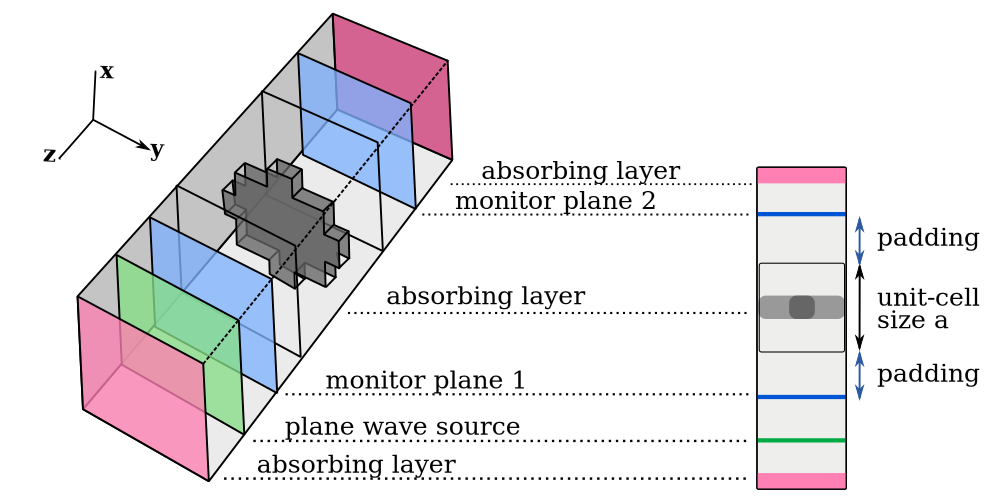
\includegraphics[width=.8\textwidth]{img/meep_geometry.pdf}  \label{fg_fdtd_sparam} \end{figure} %% 
The set-up for the scattering parameter method is depicted in Fig. \ref{fg_fdtd_sparam}. The wave is emitted from the source plane (green rectangle) in a direction parallel to the $z$-axis. The temporal shape of the waves was not critical for the simulation; a very short pulse, with a spectrum spanning from the GHz range to ca. 5 THz was used. 

Periodic boundary conditions along the $x$- and $y$-axes were set, so that effectively an infinite metamaterial slab was simulated. On both faces perpendicular to the $z$ axis we added regions denoted as \textit{perfectly matched layers}\index{perfectly matched layers} \cite{oskooi2011distinguishing} to absorb all radiation (pink areas in Fig. \ref{fg_fdtd_sparam}). The implementation is based on gradually introducing imaginary part into the voxel dimensions \cite{oskooi2010meep} to prevent reflections with an arbitrary incidence angle, polarisation or frequency of the wave.
The average electric and magnetic fields in each of the monitor planes (blue rectangles) were recorded  in each simulation step.  

Passing through the first monitor plane, the wave enters the volume of the unit cell (delimited by empty rectangles) and interacts with the structure. A part of its energy is reflected back, a part passes through and the rest may be dissipated if the structure is lossy. The fields that pass through the structure are recorded at the second monitor plane. After the energy stored in the structure drops to a small enough level, the FDTD simulation terminates and the recorded fields are processed to obtain the complex-valued reflectance $r(f)$ and transmittance $t(f)$ as functions of frequency $f$. % Before this procedure is described, a modification important for the accuracy of this set-up is discussed below.
% todo convert frequency f to omega? Why not?

%\begin{figure}[ht] \caption{An example result of a FDTD simulation (visualised using the \textit{Paraview}\index{Paraview} program). A dielectric sphere, shown in grey, was placed in a less usual, but equivalent position, across the periodic boundaries. The electric field amplitude was shown in one quarter of the simulation volume, with a clear enhancement near the dielectric surface (pink-red). % todo{replace this with a better one}
%}  \centering \includegraphics[width=10cm]{img/sim_screen.pdf} \label{fg_fdtdscreen} \end{figure} 
%}}}
\paragraph{Avoiding the near-field response in monitor planes} %{{{
\label{par_nearfield}
%% Hynek's trick
With the obvious exception of an effectively one-dimensional structure of layers perpendicular to the wave vector, all other structures will change also the orientation of the electric and magnetic fields. Such a perturbation of the field will be localized around the structure, and exponentially decaying with the distance in the form of an \textit{evanescent wave}\index{evanescent wave}.

An evanescent wave does not transport energy out of the structure into free space. However, some energy is stored in it, which can be transmitted to another structure if it approaches the zone of the evanescent wave. Even if no energy is transferred by this means, the electromagnetic behaviour of a structure is always slightly influenced by its surroundings, which manifests itself most often by the resonances shifting up or down in frequency.

The impact of the evanescent waves partially reaching the unit cell boundaries in the s-parameters method is twofold:
\begin{enumerate}
 \item{First, computing a single layer of a metamaterial unit cells, with free space in front and behind it, obviously more or less changes its behaviour compared to the periodic lattice. 

This issue is inherent to the simulation set-up, but its impact can be assessed by simulating more than one unit cell, since the retrieved values will change slightly with the number of layers being simulated: a single-cell simulation suffers the most from the absence of adjacent layers, whereas in a two-cell simulation the effect should be halved. Simulations of three (or more) cells suffer from different behaviours of the cells at the surface and inside, which possibly broadens the resonance frequency and can yield confusing results unsuitable to the retrieval method.
 } 
 \item{Second, the monitor planes cannot distinguish between the evanescent or radiated electromagnetic field, but only the radiated waves are relevant for the s-parameter computations. At very low frequencies or at frequencies close to resonances, it was observed that the near field can significantly distort the retrieved parameters.

This can be resolved by shifting both monitor planes away from the metamaterial cell by a distance denoted as \textit{padding}\index{padding}. As the evanescent field decays exponentially, padding of less than half of the unit cell size is often sufficient to suppress all artefacts due to near-field components. In contrast, propagating waves only gain an additional phase offset that can be easily compensated after the simulation. } 
 \end{enumerate}
To the knowledge of the author, such a shift of monitor planes has not been employed in any related paper. It efficiently resolves the issue, and it does so at an acceptable expense of moderately extending the simulation volume. % (todo? figure here a-b-c of different padding near a dielectric rod)

%}}}
\paragraph{Scattering-parameter retrieval procedure} %{{{
The averaged electric and magnetic fields recorded at the first monitor plane will be denoted as $E_{x}^{(1)}(t), H_{y}^{(1)}(t)$. Likewise, those at the second monitor plane will be denoted as $E_{x}^{(2)}(t), H_{y}^{(2)}(t)$. The amplitudes of typical time records are shown and commented in Fig. \ref{fg_sparam_timedomain}.  
\begin{figure}[ht] \centering \caption{Time-domain records of the fields in the s-parameter-based retrieval method; absolute values of the complex recorded fields at the first $E_{x}^{(1)}(t), H_{y}^{(1)}(t)$ and second $E_{x}^{(2)}(t), H_{y}^{(2)}(t)$ monitor plane.\\
The impinging pulse (ca. 2 ps long) excited two distinct resonances  in the structure, that both decayed exponentially in time with different decay rates, as outlined by the thin line segments. About 35 ps after the source was switched off, the stronger resonance reduces its intensity below that of the higher quality resonance, which can be clearly seen as a change of the decaying amplitude slope. The simulation duration  was $t_{sim} =$ 150 ps. \\
After 80 \% of the time record length, the field is multiplied by the smooth envelope function described by Eq. (\ref{eq_envelope}).} \includegraphics[width=.7\textwidth]{img/sim_timedomain_debug.pdf} \label{fg_sparam_timedomain} \end{figure}

The spectral resolution is determined by the length of the time record. The higher quality of resonance, the sharper its spectral features. %is equivalent to coarse sampling on the frequency axis, which cannot fully resolve the shape of the resonance. 
From the \textit{Fourier-Plancherel theorem}\index{Fourier-Plancherel theorem} %% TODO ref
it follows that the part of the electromagnetic energy that was coupled to the structure, but was not radiated back until the end of the time record, will be also missing in the spectra in the frequency domain. When the time record is too short and significantly truncates a resonance ring-down, characteristic artefacts in the spectra occur which are very detrimental to further visual and numerical evaluation. 

\label{convolringing}
Using the convolution theorem (see Sect. \ref{subsection_local_resp}), it can be deduced that clipping the recorded fields by a rectangular window in time domain introduces artefacts equivalent to convolution with the $sin(f)/f$ function in the frequency domain. Multiplication of the records with a smooth window function, known also as \textit{apodisation}\index{apodisation}, does not improve spectral resolution, but it suppresses the visually distracting \textit{ringing artefacts}\index{ringing artefacts}, which are apparent for the quadrupole resonances (see, e.g., Fig. \ref{fg_expe_fishnets}). 

To this end, all four time records were multiplied by the envelope function $g(t)$ before further processing:
\begin{equation} 
\begin{split}
	g(t) 	& = 1 \text{ for } t < 0.8 t_{sim} \\
	g(t)    & = \frac{1 + \cos\left(\pi \frac{t/t_{sim}-0.8}{1-0.8}\right)}{2}  \text{ for } t > 0.8 t_{sim},
\end{split}
\label{eq_envelope}\end{equation}
which ensured that after 80 \% of the overall simulation duration $t_{sim}$ the field starts dropping smoothly to zero, introducing a temporal envelope similar to the \textit{Hann window}\index{Hann window} function often used in digital signal processing. 

By means of the Fourier transform, the fields were converted to the frequency domain. This operation is simply denoted as $E_{x}^{(1)}(t) \rightarrow E_{x}^{(1)}(f)$, and so on. 
\begin{figure}[ht] \caption{An illustration of orientations of the electric field $\E$ (blue), magnetic field $\HH$ (light brown) and wave vector $\kk$ (thick arrow) for the waves registered in the simulation.}  \centering \includegraphics[width=8cm]{img/sim_separating_wave.pdf} \label{fg_separating_wave}\end{figure}

The monitor planes are assumed to be located in vacuum, and at a distance sufficient to eliminate the evanescent waves of the simulated structure. It follows that the vectors of the electric field $\E$, magnetic field $\HH$ and the wave vector $\kk$ must form a right-handed triplet. %% TODO reference the M. E. solution
At both monitor planes, the forward and backward waves are linearly superposed as illustrated in Fig. \ref{fg_separating_wave}. Therefore they can be separated by using the following relations: 
\begin{equation} 
	\begin{split}
		A^{\text{(in1)}}(f)  := \frac{E_{x}^{(1)}(f) + Z_0 H_{y}^{(1)}(f)}{2}, \quad \quad \quad & A^{\text{(out1)}}(f) := \frac{E_{x}^{(1)}(f) - Z_0 H_{y}^{(1)}(f)}{2}\\
		A^{\text{(out2)}}(f) := \frac{E_{x}^{(2)}(f) + Z_0 H_{y}^{(2)}(f)}{2}, \quad \quad \quad & A^{\text{(in2)}}(f)  := \frac{E_{x}^{(2)}(f) - Z_0 H_{y}^{(2)}(f)}{2}. 
	\end{split} 
\label{eq_separate_ampli}\end{equation}
The constant $Z_0$ stands for the \textit{vacuum impedance}\index{vacuum impedance}, i.e. the ratio of the electric and magnetic fields of a freely propagating wave. Its universal value in SI units is $Z_0 = \sqrt{\mu_0/\varepsilon_0} = 4\pi c \cdot 10^{-7} \approx 376.7$ $\Upomega$, but in the actual FDTD simulations, the built-in convention of $Z_0 = 1$ was used.
An example of the wave separation result is plotted in Fig. \ref{fg_ampli}.  
\begin{figure}[ht] \caption{Separated amplitudes of the forward and backward waves at the first and second monitor planes 
allow to assess the validity of the simulation results.\\
The incident wave $A^{\text{(in1)}}(f)$ should have a smooth spectrum (blue curve), as it is directly generated by a broadband source. The reflected wave $A^{\text{(out1)}}(f)$ (green curve) and the transmitted one $A^{\text{(out2)}}(f)$ (light-blue curve) appear to be somewhat complementary to each other, since squares of their amplitudes should approximately sum up to the square of the incident wave amplitude, or less in case of losses. \\
The fourth wave $A^{\text{(in2)}}(f)$ should be negligible, as almost all the wave energy is expected to be absorbed by the perfectly matched layers at the $z$-faces of the simulation volume. In practice it is nonzero, also due to numerical imprecision and remaining near-field components of the structure. This relative error in amplitude is usually less than $10^{-3}$.}  \centering \includegraphics[width=10cm]{img/sim_ampli_debug_band.pdf}\label{fg_ampli} \end{figure} 

Finally, one can easily compute the complex scattering parameters $r(f)$ and $t(f)$ as the ratios of the reflected and transmitted wave amplitudes to that of the incident wave, respectively:
\begin{equation} 
	\begin{split}
		s_{11}(f) \equiv r(f) := \frac{A^{\text{(out1)}}(f)}{A^{\text{(in1)}}(f)},\\
		s_{12}(f) \equiv t(f) := \frac{A^{\text{(out2)}}(f)}{A^{\text{(in1)}}(f)}.
	\end{split}
\label{eq_sparam}\end{equation}

%}}}
\FloatBarrier%{{{
\begin{figure} 
\caption{\textbf{(a)} Electron microphotograph of the STO array (from \cite{nemec2009tunable}), front view, 
\textbf{(b)} dimensions of one unit cell, drawn as the side view}  \centering \vspace{-4mm}
\begin{overpic}[width=.6\textwidth]{img/STOBar_photo.pdf}     \put(0,67) {\textbf{(a)}} \end{overpic}\quad
\begin{overpic}[width=.3\textwidth]{img/EBars_STO_sketch.pdf} \put(1,95) {\textbf{(b)}} \end{overpic} 
\vspace{-5mm}\label{fg_STO_bar_geom} \end{figure} 
%}}}
\paragraph{Comparison of simulated and experimental spectra} %{{{
To verify the simulation results against experimental data, we computed $r(f)$ and $t(f)$ for a structure that had been measured in our terahertz laboratory.
It consisted of an array of high-permittivity dielectric bars, cut using a femtosecond laser % todo{what was the laser power and other parameters?
from a 26 $\upmu$m thick strontium titanate (STO) slab \cite{nemec2009tunable}. The periodicity was 96 $\upmu$m and the laser cut width 30 $\upmu$m, resulting in the width of 66 $\upmu$m for each rectangular bar as shown in Fig. \ref{fg_STO_bar_geom}. 

The permittivity of STO strongly depends on the temperature, and was not known a priori, so it was chosen as $\varepsilon_r(1\text{ THz}) = 365 + 62\ii$ for the simulation to match the experimental spectra.
\FloatBarrier
\begin{figure} \caption{Experimental transmission $t_{exp}(f)$, compared with numerical reflectance $r(f)$ and transmittance $t(f)$ for strontium titanate bars with a rectangular cross-section $26 \times 66$ $\mu$m$^2$, oriented parallel with the electric field. }  \centering \includegraphics[width=12cm]{img/STObar_rt.pdf} \label{fg_STO_bar_rt} \end{figure} 

In Fig. \ref{fg_STO_bar_rt}, the curves computed using the FDTD simulations are compared with the experimental ones, showing very good match in three well-resolved resonance peaks, and high reflectance ($|r| > 0.9$) in most of the spectrum which is caused by strong impedance mismatch between the dielectric and the surrounding air.

\begin{figure}[ht] \centering \caption{
Set of simulated absorption spectra, computed as $1-|r^2|-|t^2|$, for different widths of the strontium titanate bar (in micrometers).
The experimental bar width of 66 $\mu$m is denoted by the white line. Different modes are marked by the black curves and the cross-sections of their approximate electric field shapes are drawn above the plot.} \includegraphics[width=.9\textwidth]{img/STOBarC_modes2.pdf} \label{fg_STO_bar_modes}\vspace{-5mm} \end{figure}
\FloatBarrier
%}}}
\paragraph{Example of a parametric scan with FDTD simulations} %{{{
To briefly illustrate further possibilities of the numerical simulations, in Fig. \ref{fg_STO_bar_modes} we scanned the relative width of the STO bar, and computed the relative energetic loss in the structure given by $1-|r^2|-|t^2|$. Each loss peak can be clearly associated with one resonant mode in the dielectric. Only modes with a mirror symmetry in the direction  transverse to the wave propagation couple to the wave; the remaining antisymmetric modes would manifest themselves at oblique incidence only.

The two-dimensional scan can provide further information about the underlying physics. Most importantly, it is clear that the resonance frequencies of the modes have different sensitivities to the bar width. Note that both the vertical and horizontal axes are logarithmic, so the power dependence can be directly estimated from the slope of each line. 

It can also be seen from Fig. \ref{fg_STO_bar_modes} that for the bar width close to 66 $\upmu$m, which is indicated by the horizontal white line, two modes cross-over in frequency. Namely, one of these is a narrow mode with nodal planes almost parallel to the wave propagation, while the other one is much broader one with one nodal plane centered inside the dielectric slab volume. This explains why the first resonance in Fig. \ref{fg_STO_bar_rt} has an obviously asymmetric shape, both in the simulated and experimental spectra. 

The overlap of two modes differing by the spectral widths and the resonance frequencies forms a typical \textit{Fano resonance}\index{Fano resonance} shape, which would be probably observed experimentally if the losses were lower.
A more elaborate discussion on periodic structures composed of dielectric bars/rods oriented either along the electric or the magnetic field will follow in the Sections \ref{sect_diel_rods_mag} and \ref{sect_diel_rods_el}.
%}}}
\paragraph{Retrieval of the effective parameters} %{{{
%So far, only the amplitude and phase of frequency-dependent reflectance $r(f)$ and transmittance $t(f)$ for a finite number of metamaterial cell layers were determined. 
Complemented with the cell thickness $d$, the spectra of the frequency-dependent reflectance $r(f)$ and transmittance $t(f)$ can serve as inputs for the s-parameter method,  \cite{smith2002determination, smith2005electromagnetic} \cite[pp. 51-55]{shalaev2010book}. The expression for the effective index of refraction is
\begin{equation} \Neff = \frac{\pm \arccos\left(\frac{1 - r^2+t^2}{2 t}\right) + 2\pi\,m}{k d}, \label{eq_Neff} \end{equation}
where neither the integer-valued branch index $m\in \mathbb{Z}$, nor the sign of the solution are known a priori. For the effective impedance, the sign is also ambiguous: 
\begin{equation} \Zeff = \pm \sqrt{\frac{(1+r)^2 - t^2}{(1-r)^2 - t^2}}. \label{eq_Zeff} \end{equation}

%}}}
\paragraph{Search for the correct solution} %{{{
From Eqs. (\ref{eq_Neff}) and (\ref{eq_Zeff}) it follows that the correct solution depends on three discrete-valued functions of frequency, i.e. the sign of $\Neff(f)$, its branch index $m(f)$, and the sign of $\Zeff(f)$, which have to be determined during computation.  We identified the following criteria for selecting exactly one of infinitely many solutions:
\begin{enumerate}
	\item{Passivity, i.e., inability to supply energy to the wave propagating through the structure, requires the \textit{imaginary}\index{imaginary} part of refractive index be non-positive: 
		 \begin{equation} \Neff''(f) \leq 0 \quad \forall f\in \mathbb{R} \label{eq_Neff_pass}\end{equation}
		 } 
	 \item{Passivity with regard to the wave reflected from the structure interface requires the \textit{real} part of refractive index be non-positive, too: 
		 \begin{equation} \Zeff'(f) \leq 0 \quad \forall f\in \mathbb{R} \label{eq_Zeff_pass}\end{equation}
		 } 
	 \item{A causal response of the sample requires a specific relationship between the real and imaginary parts of $r(f)$, $t(f)$ and of effective parameters $\Neff(f)$ and $\Zeff(f)$, when substituted for the function $F(\omega)$:
		 \begin{equation} 
F'(\omega) = \int_{-\infty}^{+\infty}  \frac{-2\ii}{\omega - \Omega} F''(\omega) \,\mbox{d}\Omega  \equiv  \left[\frac{-2\ii}{\omega}\right]\,\ast\,F''(\omega). \tag{\ref{eq_kkresult} \again}\end{equation} 
Perhaps the most familiar consequence of this criterion is the requirement of continuity for $\Neff(f)$ in all structures with nonzero losses.
		 } 
\end{enumerate}
Note that in the papers that use the other complex convention, i.e. $e^{-\ii\omega t}$, both passivity conditions use the opposite sign. This does not apply to the kernels of the Fourier nor Hilbert transforms.

%}}}
\FloatBarrier%{{{
\begin{figure} \centering \caption{\textbf{(a)} Real and \textbf{(b)} imaginary parts of the arccosine of complex argument $\upsilon$. Branch cuts are denoted with thick lines. The thick curve shows a possible trajectory of  $\upsilon(f)$ (upon a frequency variation), which intersects the branch cuts in points marked as R, L.\\ \textbf{(c)} From top to bottom: an example function  $\upsilon(f)$, its ordinary arccosine, example branch and sign choices ensuring the continuity of the arccosine function, and the continuous version of $\arccos_{\mathrm{c}}(\upsilon)$, as determined by the algorithm described.} \includegraphics[width=16cm]{img/continuous_arccos/continuous_arccos_new.pdf} \label{fg_arccos}
\end{figure}
%}}}
\paragraph{Retrieval of effective $\Neff'$ based on unambiguous complex arccosine} %{{{
We wrote a custom procedure to select the correct solution automatically on pure mathematical basis. To our knowledge, such an approach was not addressed in any of previously published papers. Alternative approaches are briefly discussed in the following section.

The ambiguity in Eqs. (\ref{eq_Neff}, \ref{eq_Zeff}) results from the fact that the inverse functions of arccosine and square root are not injective mappings \cite{simovski2009material}:
\begin{equation} \cos x = \cos (-x) = \cos(x+2\pi) \quad  \forall x\in\mathbb{C}, \label{eq_noninjN}\end{equation}
\begin{equation} x^2 = (-x)^2 \quad \forall x\in\mathbb{C}. \label{eq_noninjZ}\end{equation}
%Although the range of values for arccosine and square root are defined uniquely in mathematics, the retrieval algorithm described here extends these functions to yield different values to ensure continuity.
Since the temporal records of the fields are exponentially decaying functions, the reflectance  $r(f)$ and transmittance spectra $t(f)$ must be continuous. 
It is assumed that for any realistic structure with nonzero losses, the transmission never passes exactly through the complex zero, and the arccosine argument from Eq. (\ref{eq_Neff})
\begin{equation} \upsilon(f) = \frac{1-r^2+t^2}{2t},   \label{eq_upsilon}\end{equation}
is also a continuous complex function. Any discontinuities in the retrieved spectra of $\Neff'(f)$ may therefore arise exclusively from discontinuities of the arccosine function in the complex plane.

To ensure the  overall continuity of $\Neff$ in Eq. (\ref{eq_Neff}), it is therefore necessary to identify the two \textit{branch cuts}\index{branch cuts of arccosine} of arccosine in the complex plane, as illustrated in Figs. \ref{fg_arccos}a,b. Different measures must be taken for the sign and branch index $m(f)$ to ensure continuity:
\begin{enumerate}
\item{
If, by increasing the frequency, the arccos argument $\upsilon$ passes through the right branch cut at $\upsilon' > 1, \upsilon'' = 0$ (point "R" in Fig. \ref{fg_arccos}c), the real part of arccos$(\upsilon)$ touches zero, whereas its imaginary part is non-zero and changes its sign. The direction given by the sign of $d\upsilon'/df$ does not play any role. The continuity is achieved if, from this frequency on, one reverses the sign of the arccos term . 
} 
\item{
		At the left branch cut (the "L" point in Fig. \ref{fg_arccos}c), i.e., for $\upsilon' < -1, \upsilon''=0$, where the imaginary part of $\arccos(\upsilon)$ experiences again a step-like change of the sign and the real part touches the value of $\pi$. To restore the continuity, the sign reversal must be also accompanied by a change of the branch index. . 
} 
 \end{enumerate}

%}}}
\paragraph{Effective impedance retrieval} %{{{
The sign of the square root function is similarly chosen so as to ensure that $Z$ is a continuous function of frequency. Probably the simplest approach is to express the square root argument in Eq. (\ref{eq_Zeff}) in the polar nonation, i.e., as its real-valued modulus and its angle in the complex plane. The angle can be easily ensured to be a continuous function by shifting it by $\pm 2\pi$ at any discontinuity.

Using the \textit{Moivre theorem}\index{Moivre theorem}, the square root is then computed by halving the angle of the argument, and computing the square root of its real-valued modulus. Both operations are safe in terms of maintaining the continuity.

A particular implementation of this algorithm for  continuous arccosine and square root retrieval can be found online in Ref. \cite[\texttt{effparam.py} file]{dominec2014_meep_metamaterials}.

%}}}
\paragraph{Initial branch and sign choices}%{{{
Next, it is necessary to establish the sign and branch index of $\Neff$ and the sign of $\Zeff$ at the starting point of the spectrum. One can assume that for very low frequencies below any individual resonance, also the Bloch's wave vector tends to zero, $K\rightarrow 0$. In case of conductive structures, the spectrum starts with a plasma-like band gap at low frequencies, leading to an evanescent wave with vanishing wavenumber as well.

Whenever the spectra of $r(f)$ and $t(f)$ are computed using the Fourier transform, they are known also for very low frequencies and the selection of the initial branch is thus easy.

The remaining step is to establish the signs of $\Neff$ and $\Zeff$, using the aforementioned rules requiring the metamaterial passivity.

%}}}
\paragraph{Computing effective parameters of a 1-D photonic crystal}%{{{
The above described algorithm was proven to work reliably with most structures. However, it is sensitive to numerical errors 
when the arccosine argument $\upsilon(f)$ in Eqs. (\ref{eq_Neff}, \ref{eq_upsilon}) passes 
near the points $(-1+0\ii)$ and $(1+0\ii)$, that is, near the ends of the branch cuts of the complex arccosine.

Unfortunately, it was observed that $\upsilon(f)$ comes excessively close to these points in the spectra of planar slabs of lossless dielectrics, particularly when the spectral resolution is low. A correct retrieval of effective parameter spectra for this particular structure requires that even in these points, the curve is processed as if it had crossed the branch cuts. 

Otherwise, the retrieved spectrum of $\Neff(f)$ remains continuous, but at higher frequencies it ceases to make physical sense. Its imaginary part acquires the wrong sign in the band gaps, breaking the passivity criterion. Simultaneously,  in the next photonic band its real part decreases with frequency, which would break the Kramers-Kronig relations [see Eq. (\ref{eq_kkresult})] and would be a sign of negative group velocity occurring without significant dispersion. For these reasons, this error can be easily notified, and with further programming it can be combined with the verification against the Kramers-Kronig relations.

This is the only issue known to the author which arises from the described effective-index retrieval algorithm. This problem has proven to be efficiently resolved by introducing moderate losses into the structure and/or artificially shifting the branch-cut detection points to be slightly closer to the complex zero, e.g. to (-0.999+0$\ii$) and (0.999+0$\ii$). In many cases, the wrong detection of the branch was resolved simply by multiplying the recorded fields by the smooth window function from Eq. (\ref{eq_envelope}).

%}}}
\paragraph{Summary of the scattering-parameter method}%{{{
The scattering-parameter method is the most widely used one for the effective parameter retrieval. It stands out among other methods by relying on the amplitudes of the reflected and transmitted waves only, without any inspection of the fields inside the unit cell. It is also efficient, since it requires a single time-domain simulation to retrieve the full spectrum of effective parameters. The wave is let to propagate freely through the structure, and then the retrieval algorithm determines the wavenumber at each frequency component of the incident wide-band pulse. The frequency $\omega$ represents the input, and the wavenumber $K(\omega)$ is one of the outputs.

\label{sparamweaknesses}
However, the scattering-parameter method also has its weaknesses. Perhaps the worst one is that it does not fail explicitly in cases it is not appropriate for; or, as stated in Ref. \cite{markel2013current}:
\begin{displayquote} 
\textit{Of course, a refractive index per se (generally, tensorial and dependent on the direction of the Bloch's wave vector) can always be formally introduced for a Bloch's wave.}
\end{displayquote}
One has to be careful to verify whether the retrieved values of effective parameters make any physical sense whatsoever, or are just a confusing output of an algorithm used outside its scope. The majority of the possible issues was mentioned above:
\begin{enumerate}
		 \item{The method is intrinsically imprecise, because the evanescent fields of most structures are influenced by the free space in front of the unit cell and behind it. This issue can be neglected if nearly all the energy is transferred by the radiated wave, in which case the metamaterial is sometimes described as a \textit{Bloch's lattice}\index{Bloch's!lattice} \cite{simovski2007bloch, andryieuski2012bloch}. In other cases, usually in dense or metallic structures, a significant amount of energy is transferred by the near-field coupling, and it can be demonstrated that the effective parameters retrieved by this method strongly depend on the number of layers \cite{rockstuhl2008transition,andryieuski2010homogenization} which renders the approach invalid.
			 } 
		 \item{Another source of errors is the fact that the monitor planes detect also the near field, requiring one to increase the distance between the structure and the monitor planes.} 
		 \item{Although we devised a relatively robust computation of effective parameters, the current implementation is still sensitive to numerical errors when spectra of lossless dielectric slabs are computed.} 
		 \item{The method requires the structure to be symmetric with regard to the wavevector $\KK$, since it attempts to approximate it by effective parameters that leave no degree of freedom for possible asymmetry. An example of an asymmetric structure was discussed in Ref. \cite{smith2005electromagnetic}, where it was concluded that
 \begin{displayquote} \textit{\ldots so different are the two solutions for $\Zeff$ for the asymmetric structure that in general the assignment of values of $\eeff$ and $\meff$ to the composite becomes counterproductive.} 
 \end{displayquote}
 In the view of the author of this thesis, also the retrieved $\Neff$ in Fig. 7c of Ref. \cite[p. 036617-9]{smith2005electromagnetic} can be reasonably interpreted if and only if the structure is symmetric. 
			 }
	     \item{Perhaps the most fundamental limitation of this method comes from its principle of retrieving the wavenumber at a given frequency. For a periodic structure which exhibits a strong enough spatial dispersion, more than one wavenumber exist at a single frequency as shown in Figs. \ref{fg_dcll_nl}. For any frequency from such a problematic range, the retrieved effective parameters depend on the unknown ratio of the energy coupled to either of the waves. Therefore, the method is inapplicable for structures with a strong spatial dispersion. This effect is illustrated in the Results section (e.g. in Fig. \ref{fg_cdh2}).
			 }
\end{enumerate}

%}}}

\subsection{Current-driven homogenisation} 
\paragraph{Principle} %{{{
When more than one wavevector $\KK$ corresponds to a given frequency,  
a different approach to the effective-parameter retrieval must be used, for which the wavevector $\KK$ becomes the input, and the corresponding frequencies $\omega_{1\ldots\infty}(K)$  at the dispersion curves are returned as the output. 
This section describes the \textit{current-driven homogenisation}\index{current-driven homogenisation} (CDH), in which the whole simulation is computed exclusively with a single wavevector $\KK$, and the dispersion curves are reconstructed from multiple simulations differing by the wavevector. 

In this thesis, the method is described in its simplest form. More elaborate implementation is discussed in Refs. \cite{silveirinha2007metamaterial}, \cite{fietz2010current} and \cite{fietz2011homogenization}, which would enable to recover all 36 parameters that describe the influence of the fields ($E_x$, $E_y$, $E_z$, $H_x$, $H_y$, $H_z$) to the displacements ($D_x$, $D_y$, $D_z$, $B_x$, $B_y$, $B_z$), taking into account also possible anisotropy and bianisotropy.

%}}}
\paragraph{Bloch-periodic boundaries for arbitrary wave vector} %{{{
In CDH, the unit cell is simulated as being placed in an infinite lattice, neighbouring with the same cells of size $a$ in all three dimensions. To emulate such a lattice in a simulation of a single cell, all the faces of the unit cell have to be set Bloch-periodic, i.e., set to copy the field from the opposite face.

Exact copying of the fields from one side to another would require the wavevector of the Bloch's wave to be strictly $K_{xyz} \in 2\pi m/a_{xyz}$, which is, however, the known condition for a photonic band gap. Since we are mostly interested in computing the wavenumber inside photonic bands, the periodic boundaries have to allow for an arbitrary phase shift before the fields are copied:
\begin{equation} E(\rr + a_x\mathbf{x}/2) \quad\rightarrow\quad  e^{-\ii K_x a_x}\; E( \rr - a_x\mathbf{x}/2), \label{eq_phaseshiftp}\end{equation}
	where $\mathbf{x}$ is the unit vector along the x-axis, and $a_x$ are the unit cell size along this axis. The unit cell is assumed to be centered around the $x=0$ point, thus $x=\pm a_x/2$ denotes the point at the boundary, and similarly for other axes.

Positive phase advance proportional to $K_x$ is applied when copying the fields parallel to the x-axis, and negative phase retardation is applied when simultaneously copying the fields in the opposite direction:
\begin{equation} E(\rr - a_x\mathbf{x}/2)  \quad\rightarrow\quad  e^{+\ii K_x a_x}\; E(\rr + a_x\mathbf{x}/2). \label{eq_phaseshiftn}\end{equation}
A similar field-copying procedure is repeated in each simulation step for all remaining axes, $\mathbf{y}$ and $\mathbf{z}$, in the case of a 3-D simulation. 

%}}}
\paragraph{Single-wavevector source}%{{{
In order to excite the simulation volume with a single wavevector $\KK$ which complies to the Bloch-periodic boundary conditions imposed, the source volume must expand over the whole unit cell and acquire a correct harmonic modulation of its complex amplitude. While this task appears impossible by experimental techniques, it is straightforward in the FDTD simulation. The source is typically designed to be a complex-valued electric current with a given amplitude:
\begin{equation} \mathbf{J}(\rr, t) := \mathbf{x} \, e^{-\ii \KK\cdot \rr} \,j(t), \label{eq_currentsource}\end{equation}
	where $\mathbf{x}$ determines the default polarisation of the electric field and $j(t)$ is the temporal profile of the source.

Excitation of the structure with this kind of the source gave the current-driven homogenisation its name. Unlike the scattering-parameters method, in CDH the source volume coincides with the entire unit cell volume. An attempt of visualisation of this minimalistic simulation set-up is in Fig. \ref{fg_fdtd_cdh}. 
\begin{figure}[h] \centering \caption{Current-driven homogenisation set-up consists of a single unit cell with all faces set to be Bloch-periodic, with appropriate phase shift between the corresponding pair of faces. One example of the real part of the spatially varied source amplitude is sketched along the unit cell edge as the green-filled curve.} 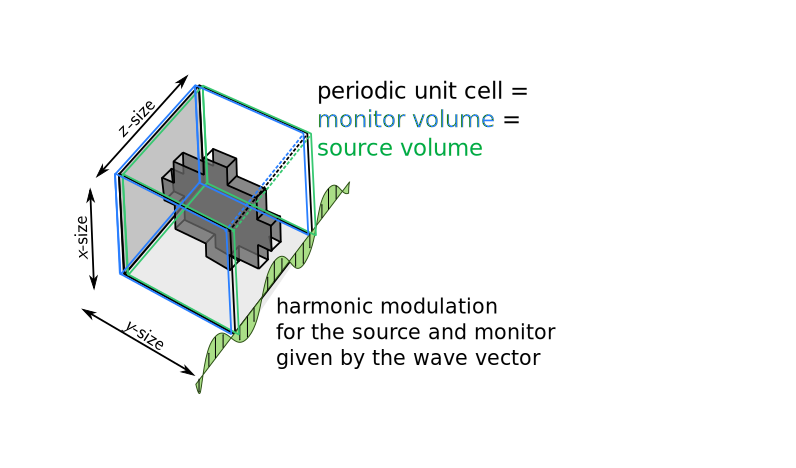
\includegraphics[width=.5\textwidth]{img/cdh_geometry.pdf}  \label{fg_fdtd_cdh} \end{figure} %% 
%}}}
\paragraph{Temporal profile of the source}%{{{
With the wavevector restricted to a single given value, it is necessary to excite and detect as many corresponding modes of the structure as possible. Therefore, a short and broadband temporal source profile could be reused from the scattering parameter method. 

Unlike the scattering-parameters method, CDH cannot detect easily the spectral profile of the exciting field, and the retrieved fields cannot be normalized against it. To maintain an approximately constant source amplitude over a wide part of the spectrum, a nontrivial temporal shape of the source was designed, tested and finally also submitted to the MEEP simulation developers:
\begin{equation} 
	j(t) := w_{BN}(t)\, \left[\mathrm{Si}(2\pi f_1 t) - \mathrm{Si}(2\pi f_2 t) \right]
\label{eq_currentsourcetime}\end{equation}
where the transcendent sine-integral function introduces the flat-top rectangular spectrum of the wave radiated from the source:
\begin{equation} \mathrm{Si}(t) = \int_0^t \frac{\sin \tau}{\tau} d\tau, \label{eq_Si}\end{equation}
	The electric field radiated by a source is proportional to the temporal derivative of the current $j(t)$ \cite{ab-initio}, therefore the sine-integral must be used to obtain the field shape of $E_x\propto \sin(t)/t$, which is known to have a rectangular flat-top spectrum.

If the source amplitude had an infinite duration in time, its spectrum would form a perfect rectangular function. However, clipping the temporal duration of the source results in spectral artefacts, as was already described on the page \pageref{convolringing}.
The artefacts can be very efficiently suppressed by multiplying the source by the \textit{Blackmann-Nutall window}\index{Blackmann-Nutall window}  function
\begin{equation} 
\begin{split} 
	w_{BN}(t) :=\; & 0.3635819 + \\
			 &+ 0.4891775\,\cos\frac{2\pi(t-t_c/2)}{t_c} + \\
			&+ 0.1365995\,\cos\frac{4\pi(t-t_c/2)}{t_c} + \\
			&+ 0.0106411\,\cos\frac{6\pi(t-t_c/2)}{t_c} \quad \quad \text{ for } t\in\langle0, t_c\rangle, \\
	w_{BN}(t) :=\;& 0 \quad \text{otherwise.}
\end{split} 
\label{eq_wBN}\end{equation} 
Since $w_{BN}(t)$ has finite support in time, but particularly fast decaying wings in its spectrum, it ensures relatively steep edges of the nearly rectangular spectrum of the source.

%}}}
\paragraph{Field monitor and identification of the dispersion curves}%{{{
The detection of the fields is defined in a way similar to the definition of the source. In each timestep, the electric field $E_x(\rr,t)$ is sampled in multiple points through the unit cell. As each of the points could have a different phase, the values are divided by $e^{-\ii \KK\cdot \rr}$ before they are averaged.

After the simulation ends, the single record of cell-averaged $E_x$ is processed to identify the set of frequencies $\omega_m(\KK)$ at which $E_x$ exhibited a ringdown. For example, if the cell is empty vacuum, the source with wavevector $\KK$ can only excite a wave at the frequency $\omega = Kc$. All other combinations of $(\omega, \KK)$ are off the dispersion curve (known also as the light line in vacuum) and no solution of Maxwell equation exists for them. Although the source can create temporary evanescent fields even at such "off-shell" combinations, the evanescent-field energy is immediately returned back to the source. 

The same holds for any kind of structure placed in the unit cell: the energy persists to the end of the simulation only at frequencies $\omega_m(\KK)$ that lie at one of corresponding dispersion curves. An intuitive way of detecting such frequencies would be to compute the Fourier transform of the recorded averaged field $E_x$ and identify the peaks in the resulting spectrum. The resolution of the Fourier transform is nonetheless proportional to the time record, and it is inefficient for the task of accurately recognizing the frequencies of a small number of damped oscillations.

A more advantageous algorithm for recognition of oscillations is the \textit{filter diagonalisation method}\index{filter diagonalisation method} (FDM), originally  developed in 1990 for analysis of experimental spectra and the nuclear magnetic resonance waveforms in particular \cite{mandelshtam1997harmonic, chao2002comparative}. Unlike Fourier transform, FDM does not require the oscillators to decay before the temporal record ends; on the contrary, it appears to work even more reliably when supplied with several tens of the oscillation periods at most. Using FDM, the simulation time could be shortened several times.

%}}}
\paragraph{Advantages over the scattering-parameters method}%{{{
Using CDH resolves some of the issues of the s-parameters method, namely 
\label{cdhadvantages}
\begin{enumerate}
\item{It simulates the unit cell embedded from all sides in the lattice, and there is no problem with the evanescent fields sensing free space as it was in the s-parameter method.} 
\item{Retrieval of the dispersion curves is not much sensitive to the actual field amplitude, but rather to the frequencies detected in its ringdown. The shape of dispersion curves is less distorted by any possible error during the scattered field detection.} 
\item{Since the wavevector is given before each simulation, no issues with wrong branch detection can flip or otherwise distort the dispersion curves.} 
\item{Also the requirements to the structure symmetry are weaker. In general, the structure is not required to have any symmetry plane perpendicular to the wavevector. Other kinds of lower symmetry may lead to bianisotropic behaviour, which would require more sophisticated detection of the waves, though.}
\item{Last but not least, CDH inherently takes into account even very strong spatial dispersion, which is not the case of the s-parameters method. All additional waves are detected correctly.}
\end{enumerate}

CDH also has more general applicability. It can operate with arbitrary orientation of the wavevector $\KK$; it can even excite longitudinal waves in the structure and retrieve their dispersion curves.

%}}}
\paragraph{Weaknesses compared to the scattering-parameters method}%{{{
The downside of CDH, as implemented in this thesis, is mainly in the fact that it provides less information than the s-parameter method: 
\begin{enumerate}
\item{It does not compute the effective impedance $\Zeff$ at all, and it is questionable whether $\Zeff$ could be computed if also the averaged magnetic field $H_y(\rr, t)$ was recorded. } 
\item{On the one hand, CDH reliably computes the dispersion curves, and the corresponding set of $\omega_m(\KK)$ functions could be inverted into $\KK(\omega)$ and, for propagation along an optical axis (cf. page \pageref{indexofrefraction}), also into $\Neff(\omega)$. On the other hand, it does not give any information on the topology of nodal planes, nor which branch of $\Neff(\omega)$ would be selected by the s-parameter method. } 
\item{We failed to obtain any useful information related to the imaginary part of $\Neff$ -- about the structure losses, field decay in photonic band gaps, and its behaviour outside the dispersion curves in general.}
\end{enumerate}
Other downsides relate to the practical implementation, and arguably are the reason for its rarer use in the literature.
\begin{enumerate}
\item{A comparable task in CDH is more computationally intensive than in the s-parameters method. For a single set of dispersion curves, several tens of simulations with different $\KK$ are needed. After they are run, a postprocessing script must analyse all recorded fields and assemble the dispersion curves. }
\item{Naturally, CDH can hardly be employed in an experiment, since it inspects the field in multiple points inside the structure simultaneously. }
\end{enumerate}
In spite of these limitations, the simplified implementation of CDH for this thesis remains an important complement to the s-parameter method. 

%}}}

\subsection{Other effective parameter retrieval methods}      % complement?
\paragraph{Extensions of the scattering parameters method} %{{{
Various modifications to the scattering parameters method were proposed, in particular with connection to the homogenisation of metamaterials. One modification makes it robust against the experimental error in the reflectance phase \cite{chalapat2009wideband}. % Wideband reference-plane invariant method for measuring electromagnetic parameters of materials
Another solution to the issues connected with experimental measurement of the reflectance was employed during the preparation of this thesis \cite{nemec2012resonant}. It involved a slight modification to the experimental set-up, and thus it is described in the experimental chapter (pp. \pageref{srtm}--\pageref{srtm2}).

Some of the modifications apply to the effective parameters retrieval only, and no change is made to the way how  the scattering parameters $r(f)$ and $t(f)$ are measured.
Not knowing the correct branch of the index of refraction is equivalent to using the folded dispersion curves (cf. Par. \ref{par_disp_curv_per}), %% TODO refer to the theory
so the post-processing of FDTD data can also be viewed as a specific, non-trivial way of \textit{unfolding}\index{unfolding} the dispersion curves. This task appears to have been often done manually, particularly in earlier papers \cite{smith2002determination}. An approach based on iterative fitting which avoids abrupt discontinuities in $\Neff'(f)$ has been published \cite{chen2004robust}, but the author conjectures that, from its very nature, it would become unstable whenever a localized resonance introduces fast changes of $\Neff'(f)$, which can be found e.g. in Fig. \ref{fg_CutWires_wireradius1u_cutwidth_comparison}. Manually assisted approaches present the risk of affecting the resulting effective parameters with unjustified subjective expectations.

A more elegant method was published in 2010 by Szab\'{o} et al. \cite{szabo2010unique} and relies on the inherently unambiguous knowledge of $\Neff''(f)$. It uses the Hilbert transform introduced in Eq. (\ref{eq_kkresult}) to recover $\Neff'(f)$ from $\Neff''(f)$. 
However, from our own experience, applying this integral transform to a finite part of spectrum introduces not only an arbitrary constant offset, but also slow continuous distortion of the $\Neff'(f)$ curves, which would require a complicated compensation.

The discussion in this thesis is restricted to the near-perpendicular wave propagation, since it is assumed the optical axis is also perpendicular to the interface. In Ref. \cite{menzel2008retrieving}, Eqs. (\ref{eq_Neff}, \ref{eq_Zeff}) were generalized also for oblique incidence. Note that for retrieving the effective index of refraction one must establish whether it makes any physical sense at all, i.e., whether the structure is either isotropic, or at least whether the angle of refraction is parallel to its optical axis (see page \pageref{indexofrefraction}).

In Ref. \cite{li2009determination}, % Determination of the effective constitutive parameters of bianisotropic metamaterials from reflectance and transmission coefficients 
the scattering parameter method was extended also to the bianisotropic behaviour of structures with reduced symmetry, and other approaches can be found \cite{andryieuski2010homogenization} in the recent literature.

%}}}
\paragraph{Averaging of the fields} %{{{
With the scattering parameters method, $\Neff(f)$ and $\Zeff(f)$ are retrieved first using the amplitudes of the reflectance and transmittance. The  local effective permittivity $\eeff(f)$ and permeability $\meff(f)$ can be  computed using  Eqs. (\ref{eq_dispeqN}) and (\ref{eq_Z}), but are considered valid only when $|\Neff'| \ll 2\pi/a$, i.e., when the unit cell size $a$ is much less than the Bloch's wavelength.

The effective parameters $\eeff(f)$ and $\meff(f)$ can however be computed directly by exciting a unit cell of the structure, averaging both the fields ($\E$, $\HH$) and the displacements ($\D$ and $\B$), and dividing the respective displacement by the field. The method is described in Ref. \cite{smith2006homogenization}, where also numerical examples are given. 

%As expected, when $|\Neff'| \not\ll 2\pi/a$ the value of $\eeff$ for wire array retrieved by this averaging method deviates from that one retrieved by the s-parameters method \cite[Fig. 5]{smith2006homogenization}. The author believes that none of methods attempting to homogenise the structure by the local parameters, $\eeff(f)$ and $\meff(f)$, can be exact.

%D.R. Smith and J.B. Pendry, Homogenisation of metamaterials by field averaging (invited paper), Journal
%of the Optical Society of America B, vol. 23, pp. 391-403, Mar. 2006.
%J. Lerat, N. Malléjac, and O. Acher, Determination of the effective parameters of a metamaterial by field
%summation method, Journal of Applied Physics, vol. 100, p. 084908, 2006.

% TODO read: http://scholar.google.cz/scholar?q=Tsukerman+2011++of+metamaterial+Rigorous+Whithey+interpolation&btnG=&hl=cs&as_sdt=0%2C5

%}}}
\paragraph{Bloch-mode analysis} %{{{
A \textit{single-interface}\index{single-interface} method has been proposed \cite{yang2010retrieving} %Retrieving the effective parameters of metamaterials from the single interface scattering problem
that analyses only the field behaviour at the interface of a semi-infinite structure.  
The fields in the structure are computed and decomposed into discrete modes of the Bloch's wave. The method attempts to recognize a dominant Bloch's mode for which the wavevector $\KK(\omega)$ is deduced.
%\cite{yang2010retrieving}LISTS: "various numerical techniques have been developed, including field averaging, 7 Bloch's mode approaches, 8–10 multipole
%expansion, 11,12 and inversion of scattering parameters."
\cite{zhang2006optical} % Optical negative-index bulk metamaterials consisting of 2D perforated metal-dielectric stacks
\cite{rockstuhl2008light} %Light propagation in a fishnet metamaterial

When no mode is clearly dominant, this method naturally cannot be used. In such a case, even the scattering parameter method fails, but its limitations of applicability are less obvious than with the \textit{single-interface}\index{single-interface} method. Failure of the scattering parameter method can be observed as contradictory results \cite{rockstuhl2008transition} from simulations of different numbers of unit cells.
In Ref. \cite{paul2011reflection} %Reflection and transmission of light at periodic layered metamaterial films
it is argued that the existence of one dominant mode is the prerequisite for the structure to be viewed as homogeneous. Refs. \cite{paul2011reflection,andryieuski2012bloch} apply the Bloch-mode analysis approach to selected structures. A direct numeric evaluation of amplitudes of the different modes in 1-D photonic crystals can be found in 
\cite{mortensen2010unambiguous}. % On the unambiguous determination of effective optical properties of periodic metamaterials: a one-dimensional case study

%\cite{smigaj2008validity} %PDF? Validity of the effective-medium approximation of photonic crystals

%}}}
\paragraph{Wave phenomena} %{{{
% (skip this?) B. Popa and S.A. Cummer, Determining the effective electromagnetic properties of negative-refractive-index metamaterials from internal fields, Physical Review B, vol. 72, p. 165102, Oct. 2005

In the \textit{Wave propagation retrieval method}\index{Wave propagation retrieval method}, proposed in Ref. \cite{andryieuski2010homogenization},
the wave impinges a thick, ideally semi-infinite, volume of the periodic structure. Since there are no repeated reflections from the second interface, the averaged field amplitude is assumed to have exponential nature: $E(z) \propto e^{-2\pi i f \Neff/c}$, and thus $\Neff$ can be reconstructed using a complex logarithm.

Like in the s-parameters method, the function of $K(\omega)$ can be resolved in a single run by using a broad band pulse. Like in the current-driven homogenisation,  the fields need to be sampled inside the structure. 
% unambiguously retrieves bulk parameters; but there is still one interface and the simulation volume is large
% it also requires in-structure inspeciton

%}}}
%   \paragraph{Multipole expansion}%{{{
%    \cite{vynck2009all} % All-dielectric rod-type metamaterials at optical frequencies
%    \cite{chipouline2012metamaterials}
%    % limited only to lateral interaction -> spatial dispersion towards the orientation of \KK (not magnitude)
%    % "there is no established consensus about how the averaging procedure has to be performed"
%    \cite{petschulat2008multipole} % PDF? Multipole approach to metamaterials%}}}
%    % todo \paragraph{Approximate analytical models} ==? multipole expansion?%{{{
%    \paragraph{Quasimode theory} 
%    %%% Andriy2010: Quasimode theory ...  is based on the maximisation of optical density of states for a metamaterial while changing İ and μ of the ambient medium. The method is computationally demanding as it requires 4-parameters optimisation for each frequency.
%    \cite{sun2009effective} % Effective-medium properties of metamaterials: a quasimode theory

%\cite{simovski2007bloch} Bloch's material parameters of magneto-dielectric metamaterials and the concept of Bloch's lattices
%\cite{simovski2009material}Material parameters of metamaterials (a review)
%\cite{simovski2011electromagnetic} On electromagnetic characterisation and homogenisation of nanostructured metamaterials

%\cite{sjoberg2005floquet}
% Elaborate mathematical treatise on this topic: 
% A Floquet-Bloch's decomposition of Maxwell's equations, applied to homogenisation " The behavior of the solutions of a PDE with rapidly oscillating coefficients, considered over distances large compared to the oscillations, is in several respects similar to the solutions of a PDE with slowly varying coefficients.   The problem of homogenisation is to find these slowly varying coefficients by an ap- propriate limit process of the rapidly oscillating ones"
%\cite{hasar2011retrieval}  Retrieval approach for determination of forward and backward wave impedances of bianisotropic metamaterials
%}}}
\paragraph{Concluding remarks}%{{{
Other homogenisation methods include the \textit{multipole expansion} \cite{vynck2009all, petschulat2008multipole}, \textit{quasimode theory} \cite{sun2009effective}, or other advanced approaches as discussed by Simovski \cite{simovski2007bloch, simovski2009material, simovski2011electromagnetic, tsukerman2011nonlocal}.
Without much exaggeration it can be concluded that there are roughly as many homogenisation methods as authors involved in the research of periodic structures. All such methods work reliably in the easy cases:
\begin{displayquote}
\textit{Homogenisation theories are typically valid when the unit-cell size is insignificant with respect to the wavelength (the zero-frequency limit) and thus might be expected to result in a poor description of metamaterials.}
\cite{smith2006homogenization} 
\end{displayquote}
Indeed, in most practically encountered metamaterials today, the wavelength is not more than an order of magnitude smaller than the unit cell. %so the homogenisation results deviate from each other. Moreover, the choices for one particular method among other is usually not justified by any rigorous basis in the literature. 

Most homogenisation methods attempt to describe the structure using local effective parameters,  $\eeff(f)$ and $\meff(f)$, which do not provide enough degrees of freedom to fully express the interaction between the medium and fields. The homogenisation methods differ by the shapes of excitation fields the structure is probed with, by the  boundary conditions that may be either partially or fully periodic, and also by the way the field is analysed. Thus, it should not be surprising that also the results strongly deviate between the methods \cite[Fig. 5]{smith2006homogenization} %% todo cite some comparison
and that they even seem to break fundamental physical postulates \cite{koschny2003resonant}, even when no mistake was made during the application of the method. 

As a matter of fact, the mistake might have been made already during the \textit{selection} of the method.

From the literature available, one can conjecture that systematic homogenisation in terms of the spatially dispersive (Landau-Lifshitz) permittivity $\epsLL(\omega,\KK)$ should prevent most striking quirks arising in the local homogenisation methods. All problems involving an interface then also need to be complemented by the additional boundary conditions \cite{agranovich2006spatial}.
However, computations and the application are more complex for the medium described by the spatially-dispersive effective parameter, than for a medium described by local parameters. This is the price that would have to be paid for its more general validity.

In this thesis, we restrict the discussion mostly to the scattering parameters method, pointing out where it is applicable, and where its results cease to make any sense. The current-driven homogenisation then remains as a good reference to compare the results with.

%}}}



\chapter{Experimental methods}
\section{Short review of the terahertz technology}
The terahertz range of the electromagnetic spectrum, spanning roughly from 100~GHz to 10~THz, has met a relatively small application potential in science and technology  as yet, compared to the development in the microwave ($<$ 100~GHz) and near-infrared ($>$ 100 THz) or optical ranges. The reason can be traced down both to the limited choice and high cost of suitable terahertz sources and detectors, and to their usually small efficiency or sensitivity. The technology and science, however, develop fast in this field, and the number of terahertz-related papers has doubled every 3.2 years \cite{lewis2014review} between 1975 and 2010.  

There is a great number of books and papers that describe different terahertz sources and detectors in detail \cite[pp. 155-158]{lee2008book}\cite{sullivan2012field,lewis2014review}
and many of them are also, with more or less detail, discussed in previous doctoral theses written in our group (\cite[pp. 2-30]{pashkin2004phd}, \cite[pp. 19-25]{nemec2006phd}, \cite[pp. 7-26]{fekete2008phd}, \cite[pp. 11-21]{sibik2010dp}, \cite[pp. 31-45]{yahiaoui2011phd}, \cite[pp. 33-38]{mics2012phd}, \cite[pp. 25-33]{skoromets2013phd}, etc.).

Electromagnetic waves in the terahertz range are radiated whenever charged particles are subject to fast-enough acceleration at the picosecond scale.  The generation processes may be sorted with regard to the medium in which the emission occurs and to the origin of the force causing the acceleration.  In the following paragraphs, we try to review the terahertz technology in a systematic manner.

Although they are widely used at higher frequencies, thermal sources are rarely used in the THz range. The black body radiation is governed by the Planck law \cite[p. 23]{klingshirn2007semiconductor}
\begin{equation}I(f, T) = \frac{2 h}{\pi^2 c^2}\frac{f^3}{e^{\frac{h f}{kT}}-1} \mathrm{\,W\,sr^{-1}\,Hz^{-1}\,m^{-2}}, \label{eq_planck}\end{equation}
from which it follows that the luminosity $I$ in the terahertz range is always very small: Integrating over frequencies from 300~GHz to 3~THz, one obtains roughly 0.6 W sr$^{-1}$ m$^{-2}$ at the room temperature ($T=$ 300~K).  Furthermore, all Planck oscillators at the frequency of e.g. $f =$ 1~THz are already fully saturated:
%  although the thermal energy at room temperature $T$ is significantly higher than the photon energy $hf$ at 1 THz
$$k_B T \approx 1.38\cdot 10^{-26} \text{ J K}^{-1} \cdot 300 \text{ K~} \approx 25.8 \text{ meV } \quad\gg\quad h f \approx 4.13 \text{ meV}, $$
and therefore the power radiated in the THz range cannot be significantly improved by increasing the black body temperature. Thus, it can be shown that in this part of the spectrum the luminosity scales only linearly with the temperature $T$; in contrast, the total power scales as $T^{4}$ as follows from the Stefan-Bolzmann law. Therefore, sources other than thermal are preferred for measurements in the THz range.

\subsection{Terahertz sources}
\paragraph{Kinetic energy of an electron beam} %{{{ ================================================================================
One class of devices uses the kinetic energy of an electron beam propagating in the vacuum. In devices accelerating a circulating electron beam, such as cyclotrons or synchrotrons, radiation is emitted when electrons are passing through the bends in the particle path, the deflection of the electrons being caused by a static transverse magnetic field. If the electrons are packed in a short bunch, it results in an efficient emission of a coherent broadband pulse. %% with an improved efficiency in THz if they are packed
Another example is the free electron laser with the electron bunches %% TODO ... forming upon ...
passing through a device with a periodically poled magnets, called \textit{wiggler}. 
Both types of devices provide an excellent brightness and tunability, but they are rather large-scale facilities often with a dedicated building. 
%In both devices, the electrons have to propagate in bunches. 

Tabletop sources of radiation covering a part of the THz range are the microwave vacuum tubes: \textit{gyrotron}, travelling-wave and backward wave oscillators (BWO, also known as \textit{carcinotrons}, of the O- and M-types), and \textit{klystron}. The unifying principle of these devices is that the electron beam speed, position or density can be modulated by the electric field, and the modulation in turn radiates amplified electromagnetic waves. Backward-wave oscillators are tunable monochromatic sources
used for continuous-wave spectroscopy, but the tunability of one device is typically limited to tens of percent and the power drops with the frequency \cite{lewis2014review}.
% M-type, the most powerful, (M-BWO) and the O-type (O-BWO). The O-type delivers typically power in the range of 1 mW at 1000~GHz to 50 mW at 200~GHz. 

%}}}
\paragraph{Terahertz solid-state oscillators}%{{{================================================================================
Reducing the size of the active regions of well-established microwave devices, such as microwave diodes, transistors and vacuum tubes, usually enables scaling down the wavelength of the emitted radiation proportionally with the dimensions. 
The fundamental issue lies in that the power drops very fast when the device is miniaturized. If the total emitted power is limited by cooling, i.e. by the surface of the active region, it drops with the second power of the device size. If the volume power density is the determining factor, the power drops even faster.  % TODO examples of dropping power
As a solution, either substantial changes in the device geometry, constituent materials, or even new physical principles have been introduced for efficient THz sources \cite[pp. 8-12]{sullivan2012field}.  

%This concept is, in fact, applicable to all % TODO is this truly 'all'?
 %devices where the wavelength is not determined by quantum phenomena, or by physical quantity other than dimension (such as the magnetic field strength in a magnetron tube).

If a relatively low power is required, principles used in microwave engineering can be extended to the lower part of the terahertz spectrum.  %% TODO stylistics
The frequency range of operation of high electron mobility transistors (HEMT) has been extended in this way up to 1~THz. %Sometimes all accompanying components are integrated to a MMIC.

An oscillator may be formed by placing an element with a negative differential resistance (NDR) into a resonant cavity or circuit. 
In \textit{Gunn diodes}, widely used in microwave technology, the NDR is due to the electron's effective mass abruptly increasing with their velocity in certain direct-gap semiconductors.
In \textit{resonant tunneling} diodes (RTDs) \cite{asada2008resonant,brown1991oscillations}, NDR is achieved by a heterostructure quantum well, where, upon an increase of the voltage, the electron energy is detuned from the resonance of the quantum well, and the current is reduced.

Yet another principle is employed in the \textit{impact ionization avalanche transit-time} (IMPATT) diodes, where a non-destructive breakdown of a reverse-biased p-n junction follows the voltage with a delay which again enables oscillations if the junction is surrounded by a cavity. 
In contrast, in the \textit{tunneling transit-time} (TUNNETT) diodes, the NDR is achieved by changing the transit time of carriers through the semiconductor volume.
%}}}
\paragraph{Nonlinear up-conversion of microwaves}%{{{ ================================================================================
A nonlinear response of semiconductor devices to microwaves can be used for up-conversion into the terahertz range. Starting from a relatively powerful and widely available semiconductor source operating in the 100~GHz range, frequency multiplying stages are often cascaded to reach frequencies several times higher \cite{thomas2012first}. 

Harmonic frequency multipliers and mixers often employ varactor diodes or Schottky diodes embedded in a waveguide. They, however, still suffer from a significant power drop above 1~THz.

%}}}
\paragraph{Nonlinear down-conversion of optical waves}%{{{ ================================================================================
The opposite approach, also known as \textit{optical rectification}, generates THz radiation as the difference frequency between two or more detuned optical waves.
The radiation may come from two lasers or laser modes, % [CCap7], 
mutually detuned by a frequency that is to be generated. %% TODO The lasers may be classical solid state, diodes or e.g. two modes in one infrared QCL. %% TODO cite one classical, and the QCL
Other possibility is to use the \textit{terahertz parametric generation} where a single wave enters the nonlinear crystal as the \textit{pump} and the second wave, \textit{idler}, is generated during the nonlinear process. The \textit{idler} wave is kept in an optical resonator; the terahertz output can be tuned by changing parameters of the resonator. 
For nonlinear generation of pulses in the THz range, usually a mode-locked laser is used that emits pulses that intrinsically cover a broad spectrum of frequencies (e.g. typically over 360--390~THz for a titanium-sapphire laser). The difference frequencies are generated from all optical frequency components simultaneously, which results in a terahertz pulse with a very broad spectrum given by the type of nonlinear medium. 

The classical process of nonlinear optical conversion involves transparent electro-optic crystals, where some measures are taken to account for the generally different velocity of all interacting waves.
\begin{itemize}
	\item{For the difference-frequency generation between optical waves of close frequency, the classical condition of \textit{phase synchronization} is equivalent to ensure similar \textit{group} velocity at the optical and terahertz frequencies. Among the materials satisfying these requirements, zinc telluride (ZnTe), gallium selenide (GaSe), and lithium niobate (LiNbO$_{3}$) % [CCap19]) 
found their widest applications in the frequency ranges up to 3--5 THz. } 
\item{The \textit{quasi-phase-matching} technique allows to compensate the difference of the group velocity of the optical wave and the terahertz wave by periodically altering the nonlinear coefficients of a crystal so that the nonlinear contribution to the resulting wave never reverses its sign. Crystals of \textit{periodically poled lithium niobate} (PPLN) are often used for this, with the possibility of shaping the poled regions as wedges (\textit{fanned-out PPLN}), which allows to change the effective poling pitch. This method is suitable for continuous-wave or narrow-band pulse terahertz generation.  }  % TODO cite 
\item{A sufficiently strong nonlinear interaction, on a length scale smaller than the coherence length, alleviates the requirements of both phase matching and low absorption of the waves \cite{leitenstorfer1999detectors}. Organic crystals, e.g. those of DAST,\footnote{DAST is a shortcut for 4-dimethylamino-N-methylstilbazolium tosylate}
%% and derivatives of MNA (2-methyl-4-nitroaniline) [CCap25]
have been reported \cite{han2000use} %[CCap24]
to have their electrooptic coefficients  two orders of magnitude higher than the materials usual in nonlinear optics, making them suitable for operation up to 20 THz. 

Nonlinear interactions in semiconductors are enhanced when the incident photon energy is above their band gap. Common crystals used for \textit{resonant THz emission} are GaAs, %[CCap22] 
InP  or CdTe (with band-gaps of 1.42, 1.34 and 1.5 eV, respectively), which can be illuminated by a titanium-sapphire laser (with an average photon energy $hc/\lambda \approx$ 1.5 eV).} 
\item{With a proper spatio-temporal optical pulse geometry and choice of materials, THz pulses can be generated  in the form of Čerenkov cone  \cite{auston1984cherenkov} even if the optical group velocity is higher than the terahertz one.}
\item{Finally, plasma generated in gases by high optical intensity of optical pulses can serve as a nonlinear medium, with low dispersion and thus a very broad bandwith of tens of THz \cite{loffler2000generation,chen2007terahertz,tong2012}. }
 \end{itemize}
%% TODO Sub-cycle control of terahertz high-harmonic generation by dynamical Bloch oscillations
%% TODO and also http://www.nature.com/srep/2014/140605/srep05045/full/srep05045.html#close

%}}}
\paragraph{Photoconductive sources}%{{{ ================================================================================
Terahertz waves can be generated by \textit{photoconductivity}, i.e. by transient acceleration of charges upon optical illumination.
%In a non-saturated regime, the change of conductivity is roughly proportional to the light intensity, and thus to the square of the electric field amplitude. In this respect, the photoconductivity is similar to the aforementioned mechanism of the second-harmonic nonlinear interaction. 
In the photoconductive devices, the major part of the energy is supplied by the external quasi-static electric field, which reduces the requirements for the laser illumination intensity. The light sources can be again two detuned lasers or laser modes \cite{gu1999generation}, or pulses from a mode-locked laser oscillator. Obviously, this method requires the photon energy to exceed the band gap of the selected semiconductor.

The photoconductive emitter is usually a slab of a suitable semiconductor with an antenna structure, deposited on the illuminated side \cite{auston1984picosecond}. Earlier antenna designs use two metallic segments of different shapes, such as split-H shape or a spiral. The gap between the electrodes may vary; the \textit{large-aperture} emitters with gaps of several millimetres 
allow to increase the energy and directivity of the THz radiation in the pulsed regime, however they require a high-voltage power supply.
The optical beams (continuous or pulsed) are always more or less tightly focused to the gap between the electrodes. 

The \textit{interdigitated emitters} \cite{darrow1990subpicosecond,hu1990optically} 
provide a large-aperture and relatively high-energy THz pulses even with low voltage in the range of tens of volts. The metallisation on its front side forms a dense array of narrow metallic wires; every second gap between them is covered with opaque paint. The odd and even wires are connected to two terminals of a voltage source.  Upon pulsed illumination, all charge stored in the interdigitated electrodes discharges through the illuminated parts of the semiconductor surface, emitting THz waves polarized perpendicular to the wire grid.

The emission efficiency can be improved when the sharp current rise is followed by a similarly sharp falling edge of the current, again in the order of one picosecond. For this purpose one needs to select a material with a very short lifetime of carriers, but a relatively high mobility thereof. Radiation-damaged silicon films on sapphire, or gallium arsenide slabs with lattice disordered either by (Be or Cr) doping, or by growing at low temperature, are used to this purpose. 

A weaker THz emission can also be observed from semiconductors even with no static bias voltage, owing to the surface electric field, photo-Dember and other phenomena \cite{corchia2001effects, heyman2001terahertz}.
%%% todo understand this more  HN: "surface depletion field in semiconductors can serve for carrier acceleration, avoiding the necessity of using an external voltage source" \cite{liu2003terahertz,zhang1992optoelectronic}
%%%   HN: "several mechanisms responsible for the enhancement depending on the excitation intensity" 

%}}}
\paragraph{Terahertz lasers}%{{{  ================================================================================
Continuous gas terahertz lasers use stimulated emission from quantum transitions between discrete rotation levels of small organic molecules \cite{chang1970cw}. Although they represent high-brightness continuous sources at multiple lines in the terahertz range, they are rather expensive and their quantum efficiency is poor, as they usually have to be pumped by a powerful carbon dioxide laser at 33 THz.

Solid-state terahertz lasers are represented by the p-doped germanium laser, where the quantum transition occurs between energy levels of light and heavy holes in a strong magnetic field and at cryogenic temperatures. The transition frequency can be continuously tuned by the magnetic field.

Quantum cascade lasers (QCL) are composed of hundreds of semiconductor layers \cite{yin2012terahertz}, which create multiple closely-spaced quantum levels. Each electron or hole travelling across the structure thus undergoes multiple transitions. Such devices are compact and  efficient sources of continuous and slightly tunable radiation in the mid-IR region. The extension of their operation under 2 THz oftentimes requires cryogenic cooling and is subject to intense research.
%}}}
\paragraph{Other THz sources}%{{{ ================================================================================
Although a complete list of all physical phenomena that lead to possibly useful emission of terahertz waves is beyond the scope of this thesis, we try to point out some most notable examples of these. 

Earlier in our laboratory it was observed that an oblique impact of femtosecond optical pulse on a 50-150~nm thick gold layer on glass emits a THz pulse of similar energy as those from an interdigitated emitter \cite{kadlec2004optical,kadlec2005study}. Other experiments, e.g. with thin organic layers \cite{ramakrishnan2012surface}, suggest the process may be intensified by surface plasmons.

Tunable terahertz continuous-wave emission was observed in multiple stacked Josephson junctions \cite{ozyuzer2007emission}, where the oscillation frequency is determined by the junction voltage $f(U) = 2e/h$, thus 2 mV correspond to roughly 1 THz. This method however requires cryogenic temperatures as a superconductor structure is used, and is still subject to primary research.

The \textit{Smith-Purcell} effect is observed when a relativistic electron beam passes close to a corrugated surface, e.g., that of an optical grating. The emitted coherent radiation can be obtained also in the THz region \cite{doucas1992first} (as determined by the grating pitch). A similar effect was later observed from a direct current flowing through a graphene monolayer placed over a photonic crystal \cite{tantiwanichapan2014graphene}.
%% TODO add: GEME coherent?, 
%% TODO add: THz HHG? http://www3.imperial.ac.uk/newsandeventspggrp/imperialcollege/naturalsciences/physics/exssseminars/eventssummary/event_21-10-2014-13-26-55
%}}}

\subsection{Terahertz detectors}
\paragraph{Thermal detection}%{{{
A broad class of detectors, applicable also to the terahertz range, measure the energy of the radiation. 
Classical bolometers use thermistors or thermocouples, resistivity of which will change when they are heated by radiation.
Pyroelectric detectors convert the heat directly to the electric signal by means of a crystal that changes its polarisation with temperature. In the Golay cells, an incident terahertz pulse heats the air and its thermal expansion is detected. Such devices usually operate at room temperature.

The concept of a bolometer can be greatly improved, in terms of sensitivity or speed, at cryogenic temperatures when a superconductor near its critical temperature or a doped semiconductor are used as the temperature detector. In the \textit{hot-electron} bolometers, the superconductor forms a narrow bridge between two contacts so that the changes in resistance are more pronounced. The changes in the superconductor behaviour can also be detected by a superconducting quantum interference device (SQUID).  

%}}}
\paragraph{Heterodyne mixing}%{{{
A continuous-wave terahertz signal can be mixed with the signal from a local terahertz oscillator, producing a difference frequency in the microwave spectral range which can be processed easily using an oscilloscope or a spectral analyzer. The nonlinear components often used up to 1 THz are Schottky diodes or superconducting Josephson junctions \cite{face1986high}.
Fast enough thermal detectors, such as hot-electron bolometers based on Nb or NbN superconducting transition, can also be used, offering higher sensitivity \cite{lee2008book}.

%}}}
\paragraph{Time-resolved field sampling}%{{{
Another class of terahertz detectors enables measuring the electric field $\E(t)$, or magnetic field $\HH(t)$, as a function of time. An important advantage of such devices is the possibility to recover the instantaneous amplitude of the field, i.e., both its modulus and phase in the frequency domain). It also allows to synchronize the detection with the pulsed source to record short terahertz transients. It should be noted that the measurement of the transmittance phase can be accomplished with a continuous tunable source, too, using a Mach-Zender interferometer.
Pulsed measurement is however vital for transient dynamics investigation.

Most of such detectors require a simultaneous incidence of the terahertz pulse and of a \textit{sampling} (or, \textit{gating}) optical pulse. The mutual timing of the pulses can be scanned using an optical delay line, thus the terahertz waveform can be recovered over repeated measurements \cite{wu1996ultrafast}.  % ist it appropriate?
Alternatively, various single-shot detection schemes have been also implemented, usually being based on the temporal dilation (chirp) of the sampling optical pulse and subsequent spectral analysis of the output.
% TODO check the THz detectors as I proposed
% HN: In the other configuration the ellipticity is measured near the zero-transmission point (Fig. 1.3b) [hn54]
% HN: this scheme is important when a single photodetector is required, like in certain imaging applications [hn55] or in single-shot measurements [hn56]
The physical process of the optical sampling is in most cases analogous to one of the above described mechanisms of terahertz pulse generation:
\begin{enumerate}
 \item{Photoconductive receiving antennas use a short optical pulse to introduce a subpicosecond time window to short-circuit the antenna segments. The instantaneous THz field at the time of the optical pulse arrival moves a charge across a semiconductor gap between two metallic stripes. The charge amount is proportional to the THz field and  can be amplified and measured by relatively slow electronics.} 
 \item{Electrooptic sampling uses the nonlinear interaction between the optical and THz electric fields in an electrooptic crystal, typically a thin plate of ZnTe. To discriminate between the sampling optical pulse and the weaker component added to it by the nonlinear interaction, usually a change of optical polarization is detected.}  % todo add that this will be discussed?
 \item{Magnetooptic sampling was also demonstrated \cite{riordan1997free}, based on the Faraday rotation induced by the magnetic component of a transient THz wave.}
 \end{enumerate}
Similar to all cases of the pulsed terahertz sources, the temporal resolution of sampling terahertz detectors is generally limited by the duration of the sampling optical pulse, and more often, by the limited speed of the photoconductive antenna or by the group velocity dispersion of the nonlinear crystal. The detection bandwidth can be improved using the approaches used in the terahertz pulsed sources  such as the use of thin plates of organic crystals (DAST) % CITE
or nonlinear detection in plasma.
%% 
%% %TODO about synchronicity - almost always pumped/triggered by a pulsed laser
%% \mdf{
%% "The THz radiation is generated in a large area THz emitter"
%% %\cite{12   A. Dreyhaupt, S. Winnerl, T. Dekorsy, and M. Helm, “High-intensity terahertz radiation from a microstructured large-area photoconductor,” Appl. Phys. Lett. 86, 121114-3 (2005).}
%% 
%% distance between the parabolic mirrors is set to be 2f
%% %\cite{14   P. U. Jepsen, R. H. Jacobsen, and S. R. Keiding, “Generation and detection of terahertz pulses from biased semiconductor antennas,” J.  Opt. Soc. Am. B 13 (11), 2424-2436 (1996)}
%% 
%% finally focused onto a (110) ZnTe detector crystal
%% %\cite{13   G. Gallot and D. Grischkowsky, “Electro-optic detection of terahertz radiation,” J. Opt. Soc. Am. B 16 (8), 1204-1212 (1999).}
%% }

%}}}


\section{Terahertz time-domain spectroscopy} \label{sect_tdts} 
\paragraph{Overview of the method}%{{{
The numerical data presented in this thesis could be in some cases corroborated by experimental measurements using the \textit{time-domain terahertz spectroscopy}\index{time-domain terahertz spectroscopy} (TDTS) in our laboratory. 
% Note: it would be useful to find: Grüner - 1998 - Millimeter and Submillimeter Wave Spectroscopy of

The basic principle of the measurement is similar to the scattering-parameter retrieval in FDTD simulations presented in Chapter \ref{chapter_sparam}.
 A short, broadband pulse impinged the sample, one part of its energy was transmitted, another reflected and the rest was dissipated in the sample. The transmitted pulse was then recorded by the time-domain sampling setup, and processed to obtain the transmittance amplitude and phase as functions of frequency.

The reflectance could not be directly measured in the setup described, but at the end of this section an indirect method is described that allows to compute the equivalent sample properties from the subsequent echoes that arise when the sample is surrounded by thick transparent slabs of sapphire. 
In the following, we give details on the optical and terahertz experimental setup.
%}}}
\paragraph{Terahertz pulse generation}%{{{
As the source of ultrashort optical pulses, we used the commercial \textit{Coherent Mira} titanium-sapphire femtosecond oscillator with a mean power of 0.5 W, central wavelength 810 nm, repetition rate of 76 MHz and pulse duration not exceeding 70 fs.  
% \cite{pashkin2004phd} In our TDTS measurements femtosecond laser ”Mira Seed” by COHERENT has been used for generation of ultrashort light pulses with following characteristics:
	%pulse length			50 - 80 fs
	%spectral bandwidth		15 - 40 nm	
	%repetition rate			76 MHz
	%energy per pulse		8 nJ      	
	%average power			650 mW
	%pulse peak power		140 kW    	

The laser output was split into two branches at the beamsplitter (BS1 in Fig. \ref{fg_exp}), one of which was used for the electrooptical sampling setup. The major part of the energy passing through BS1 was converted to terahertz pulses using an \textit{TeraSED} interdigitated photoconductive emitter, described in the previous section. 
The voltage at the emitter was 15-20 V, and its polarity was modulated at the frequency of 91-92 kHz. This enabled us to use synchronous lock-in detection to increase the signal-to-noise ratio of the detection system. % as described below.
% TODO ADD figure of the pulse and the spectrum

%}}}
\paragraph{Vacuum chamber and sample holder}%{{{
The diameter of the active region on the \textit{TeraSED} emitter was comparable with the longer-wavelength components of the THz pulses, so the beam diffraction led to a broad angle of the terahertz emission, of the order of 0.5 radian. Therefore, the waves were reflected at an ellipsoidal % TODO check if it was not paraboloidal
 mirror and refocused at the sample. Upon passing through it, they diffracted again and were collected by an identical ellipsoidal mirror and focused at the detector. 
To allow enough clearance for a bigger instrumentation surrounding a sample, such as a liquid-helium cryostat or a heating furnace, the ellipsoidal mirrors were separated by 0.3 m and the whole beam path approached 0.6 m. % TODO check with a ruler

Propagation of terahertz waves in air over such a distance is impeded by absorption of water vapour, which is the only polar molecule found in the air in a significant concentration. The absorption forms clear notches in the terahertz transmittance spectra, for instance around 0.62, 0.75, 1.07 and 1.41~THz, which can be traced down to discrete rotational levels of the water molecules \cite{exter1989}. In the time domain, the absorption manifests itself as an exponentially decaying ringdown. %that has polarity opposite to the main THz peak.
% TODO figure from my web
In order to avoid such a signal deformation,
the whole terahertz wave path has to be in an environment free of water vapour, and the fastest way to achieve this reliably was to enclose the emitter, mirrors, sample and detector in a vacuum chamber evacuated by a two-stage rotary pump. 

%}}}
\paragraph{Terahertz detection setup}%{{{
\begin{figure}[ht] \caption{Experimental setup for the terahertz time-domain spectroscopy. BS1 is the beam splitter separating the pump and sampling branches, F1 a focusing lens, QWP a quarter-wave plate, PBS a pellicle beam splitter.  ZnTe denotes the optoelectric crystal, C is the Babinet compensator, WP is the Wollaston polarizer and PD1, PD2 and PD3 are photodiodes.} \label{fg_exp} \centering 
	\includegraphics[width=\textwidth]{img/exp_THz_sampling.pdf}
\end{figure}

Before the laser pulse entered the vacuum chamber to induce the photoexcitation of the THz emitter, a small part of its energy was separated by a reflection from a beam splitter (BS1 in Fig. \ref{fg_exp}) into the \textit{sampling} branch. 

The pulse in the \textit{sampling} branch reflected from a pair of mirrors on a delay line, acquiring a precisely controlled relative delay against the terahertz pulse. Then it was attenuated at a filter (F1) and its polarisation was converted from linear to the circular one on a quarter-wave plate (QWP). The pellicle beamsplitter (PBS) directed the optical beam along the axis of the terahertz beam. 

We used the electrooptic sampling mentioned in the previous chapter: The electric field of the terahertz pulse induced a slight transient change in the permittivity tensor of the zinc telluride crystal (ZnTe). The much weaker and shorter optical pulse was modified by this change, acquiring diagonal ellipticity that could be fine tuned for zero signal with the Babinet compensator (C). The Wollaston prism (WP) was used to separate the two diagonal components of the resulting elliptic-polarized light. The difference between these two signals, if a small modulation is assumed, is proportional to the amplitude of the electric field. This allowed us to sample the electric field with a theoretical temporal resolution given by the duration of the optical pulse, but using a standard intensity detection using a pair of silicon diodes.   
%% TODO add references to other papers and theses from our group - one cannot describe everything from Gouy shift to PKGraph ...

%}}}
\paragraph{Signal processing and acquisition}%{{{
To reduce the noise, synchronous detection with the \textit{Stanford SRS360} lock-in amplifier was used and the polarity of THz waveforms was modulated by the voltage at the TeraSED emitter. The difference signal at the two photodiodes, PD1 and PD2, was first fed to an analogue filter (with center frequency 91.3 kHz and 3 dB drop at $\pm$ 7 kHz), sampled by the lock-in amplifier and digitally normalized against the signal measured by the auxiliary photodiode PD3. The normalisation was necessary due to the fact that the difference signal is proportional not only to the terahertz field, but also to the laser intensity which may fluctuate over time. 

%The time constant of the lock-in acquisition was comparable to the time which was needed by the delay lines to introduce a picosecond delay. As a result, the speed of delay lines movement suppressed the high-frequency components of the detected signal. Attention must be paid at precise control of the delay line speed and software compensation of the artifacts.

The spectral response of both the emitter and electrooptic sampling substantially influenced the measured sample spectra. Moreover, the phase of the recorded waves was modulated, too, as a beam passing through a focus acquires additional phase due to the Gouy shift \cite{kuzel2010gouy}. Every transmittance measurement was therefore normalized in frequency domain against a corresponding free-space reference, so that both the amplitude and phase artifacts cancelled out. 

%}}}

\subsection{Simultaneous reflectance and transmittance measurement}
\paragraph{Principle} %{{{
\label{srtm}
With rearrangement of optics, it would be possible to measure the \textit{reflectance spectrum}, similarly as the transmittance was measured. However, due to the complexity of such a setup and its very high sensitivity to the sample displacement, we did not use a second sampling branch for detecting the reflected signal. Instead of using two sampling schemes, we recovered the amplitude and phase reflectance of the sample by stacking it between a pair of thick (3 and 6 mm) sapphire slabs \cite{nemec2012resonant}. Thanks to the relatively high refractive index of sapphire in the terahertz range along the optical axis, $N \approx$ 3.068, these slabs introduce several time-delayed pulse reflections, also called echoes, into the transmitted signal.
%\begin{figure} \caption{A broadband pulse passes through a single layer of microspheres randomly arranged between two sapphire slabs and is sampled by electrooptical detection.}  \centering 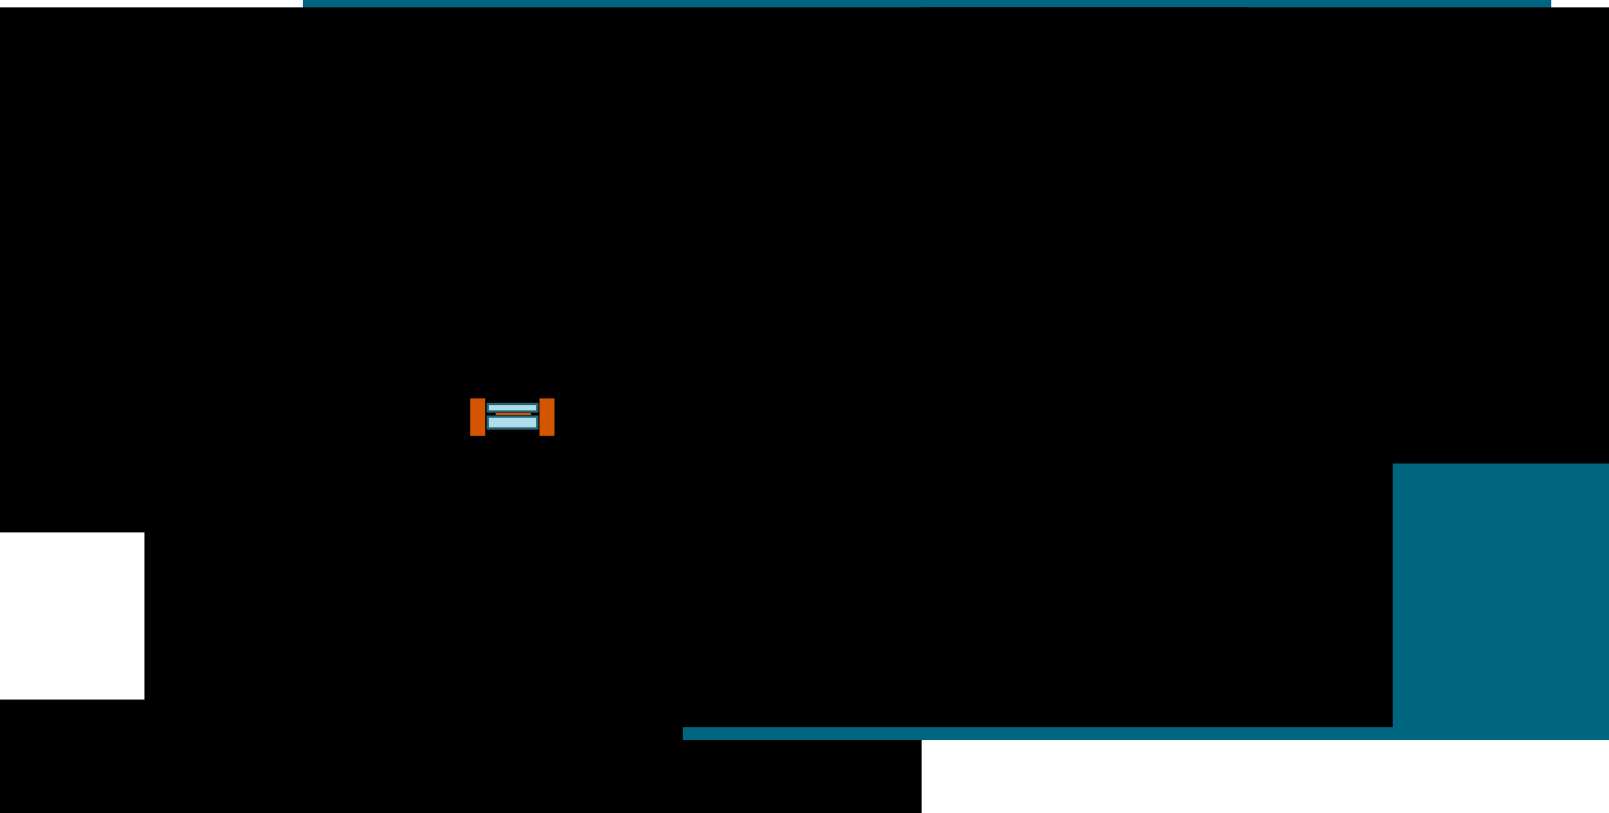
\includegraphics[width=12cm]{img/expe/sample_sapphires.pdf} \end{figure}			%% TODO no use for this figure?

If the beam divergence is neglected, each optical element can be characterised by its complex transfer function in the resulting spectrum. One needs to define three intrinsic transmittance functions: that for the beam passing through the volume of the thin sapphire $A(f)$, the one of the thick sapphire $B(f)$ and one through the thin sample $t_S(f)$; all of these are without the effect of reflection at interfaces. 

The reflection is described by two reflectance functions for the beam reflected on sapphire-air interface $r_{A}(f)$ and on the sapphire-sample interface $r_S(f)$.

By measuring the references of the thin and thick sapphires separately, the spectra of $A(f)$ and $B(f)$ as well as $r_{A}(f)$ can be established \cite{nemec2012resonant}. 

%defines the temporal separation between the main pulse and the first echo.  The reflectance and transmittance of the sample can be simply reconstructed using numerical deconvolution. The results of this method were, unfortunately, less than ideal. Among the reasons may be the possible asymmetry of the studied layer between the slabs, beam divergence and very low signal of both transmittance and particularly reflectance in the stop-bands of the sample.

To retrieve the characteristics of the sample, i.e. $t(f)$ and $r_S(f)$, the overall transmitted time-domain waveform of the sapphire-sample-sapphire structure has to be split into two parts that correspond to the direct pass, and the first echo arising from the pulse reflecting back and forth  in the thin sapphire.
The double propagation delay through 3 mm of the thinner sapphire is roughly 70 ps, which limits the spectral resolution to 14~GHz. All spectral features in the sample transmittance must be significantly broader than this value. Otherwise they could not be resolved, and even more importantly, their temporal ringdown would overlap in the time domain with the following echo and produce spurious results. Using a thicker sapphire could improve spectral resolution of this method, however it conflicts with the requirements of the terahertz beam fitting into the area of the sample \cite{nemec2009tunable} and of reducing the error caused by beam diffraction as noted in the following paragraph.

%}}}
\paragraph{Limitations of the scheme} %{{{
In the experiment, we observed substantial deviation  % TODO add some experimental data to {results} and  reference them here
from the numerically predicted results, which were moreover sensitive to subtle changes in the parameters. We propose  several independent explanations for the experimental errors:
\begin{enumerate}
\item{The geometrical beam divergence cannot be fully compensated by the transfer functions of separate sapphire slabs, $A(f)$ and $B(f)$. 
The terahertz beam is relatively tightly focused, and the focus of the echoes is longitudinally displaced compared to the focus of the first pulse. 
The deconvolution algorithm can compensate for slight focus displacement by changing the amplitude  of different frequency components, or shifting them in phase. 

However, due to the hyperbolic shape of the Gaussian beam, with its Rayleigh length $z_{R}$ being similar to the sapphire thickness\footnote{As an approximate example, for the main frequency component $f =$ 1.5~THz with wavelength $\lambda = c / f \approx 200$~$\upmu$m, for $\vartheta \lesssim 0.15$ rad as an estimated divergence of the beam from its axis, the Rayleigh half-length of a Gaussian beam would be $z_{R} = \frac{\lambda}{\pi \vartheta^{2}} \gtrsim 2.8$ mm, i.e. roughly the thickness of the thinner sapphire.}, the overall effect of two sapphires cannot be linearly compensated from two separate measurements of each of them.} 
 \item{The possible asymmetry of the sample with regard to the beam axis can substantially bias the measured reflectance. This happened during the characterisation of the dielectric spheres, when the sapphire distance was defined by a $\approx$60$\upmu$m teflon spacer. The nonuniform size of the resonators required us to attach them to one of the sapphire windows. While the spheres with the 60$\upmu$m diameter were placed symmetrically in the gap, the smaller spheres had an asymmetric position. Since the latter have higher resonant frequencies, the effect of asymmetry was probably also frequency dependent. } 
 \item{The sapphire slabs can influence the near field of resonances in some samples, cf. Sect. \ref{par_nearfield}. This error should not be significant in transversally homogeneous samples (i.e. slabs), nor in samples that are made of dielectrics with much higher permittivity than that of sapphire. However for some samples, such as metallic resonators, the spectra are be completely changed in the vicinity of a dielectric (see its application on a fishnet sample in Fig. 4.19 in Ref. \cite{yahiaoui2011phd}). }
 \item{Finally, it follows from Eq. (\ref{eq_Neff}) that reliable reflection data can only be retrieved at frequencies where also the transmittance amplitude is strong enough for the signal not to be dominated by noise. }
 \end{enumerate}
\label{srtm2}

%}}}

\section{Preparation of the titanium dioxide microspheres}
\paragraph{Fabrication through the spray-dry technique}%{{{
The collaborating laboratory of Dr. Patrick Mounaix in France %% Todo reference to Patrick's group somehow, and mention Oleg Mitrofanow (here, or later)
provided us with high-permittivity TiO$_{2}$ spheres with the sizes from 30 to 100 $\upmu$m, which were examined by the terahertz spectroscopy as dielectric resonators, and as possible constituents of a metamaterial with negative effective permeability.
\begin{figure}[ht] \caption{Microphotograph of the TiO$_{2}$ spheres after preliminary sieving} \label{fg_microphoto} \centering 
\includegraphics[height=5cm]{img/microscope_TiO2_particles.pdf}
\end{figure}

Compared to most metamaterial designs, the fabrication of the dielectric spheres can be extremely simplified by the \textit{spray-drying}\index{spray-drying technique} technique. In contrast with the expensive and time consuming \textit{top-down} processes such as laser cutting, litography or polishing, this is a typical \textit{bottom-up} process, where the particles are formed all within one procedure, though certain postprocessing is needed. 

As a first step, rutile (TiO$_{2}$) was ground to a sub-microscopic powder \cite[pp. 91-93]{yahiaoui2011phd}. A suspension of this powder in ethanol was sprayed into flame. It immediately formed spherical droplets, which dried up and sintered in the hot air. Rutile concentration in the suspension, feed rate and gas flow in the flame determined the average size of the sintered particles.

The resulting particles were annealed in a furnace to further solidify. The degree of recrystallization could be controlled  by the temperature of the furnace from 1200 to 1400 $^{\circ}$C from microscopic grains to few large crystalline domains in one microsphere. Note these temperatures used are still far below the melting temperature of rutile, which exceeds 1800 $^{\circ}$C.
Similar TiO$_{2}$ microspheres are also available commercially (e.g. from Brace, GmbH), and they were likely made with a similar process.

The annealed spheres were further treated with the aim to break or eliminate clusters, by means of light milling with agathe mortar, which was separated afterwards by ultrasound bath cleaning in ethanol. Pre-sieving was performed on commercial sieves with 100, 53, 50, 40 and 38 $\upmu$m size of the square hole, though these nominal parameters of sieves should be in no way understood as hard limits for the particle sizes. The procedure of milling, cleaning and sieving was repeated 2-3 times, according personal communication with Dr. Patrick Mounaix and {Dr.} U-Chan Chung.

Only the low-temperature annealed samples were measured by the terahertz spectroscopy in this thesis. The fine-grained rutile was assumed to represent a nearly isotropic dielectric. We estimated the size of the constituent crystalline grains by grinding one microsphere and observing it under a polarizing microscope: unlike polycrystalline aggregates, small rutile monocrystals appear as coloured particles due to their inherent birefringence. In this way, the sizes of crystalline grains were assessed to be in the order of few micrometres or smaller.

%\textit{
%(\ldots) As the spheres have been sintered at high temperature, they have been separated from a platinum plate with a small soft paintbrush followed by a light milling with a agathe mortar. The goal was to separate the spheres that are welded to their neighbours due to the sintering step. All the spheres were treated in ultrasound bath using ethanol as a liquid phase. After natural drying, the sieving was performed. (\ldots) square (or rectangular) holes sieves were used. The meshes used were 106, 100, 53, 50, 40 and 38 micrometre. As a dry sieving step was performed, the particles were light milled again in order to try to break possible agglomerates which would not go through the mesh. This process was repeated 2-3 times and a final wet sieving with ethanol was performed in order to "wash" the spheres. No special measures were taken according to their shapes. (\ldots) } 
% TODO


%}}}
\paragraph{Theory of anisotropic sieves}%{{{
Triple sieving on commercial sieves, weaved from stainless steel wire, did not provide narrow enough size distribution, which is however essential for obtaining a narrow resonance peak of the sample. We therefore developed a more exact method for very fine sample sieving and characterisation. 

\begin{figure}[ht] \caption{Correspondence between the hole shape (above) and the set of ellipsoids that can pass through the hole (below), determined by their medium and minor axes. Somewhat surprisingly, the \textbf{(a)} square and \textbf{(b)} lozenge holes result in circular/elliptic set of passing particles, whereas the \textbf{(c)} circular and \textbf{(d)} elliptic holes result in the square/rectangular shape of such an region.\\
For clarity, some limiting-case examples of the ellipsoid projection and the equivalent position on the minor-major ellipse axis plot are drawn in blue, violet and red. } \label{fg_sieve_pass_notpass} \centering 
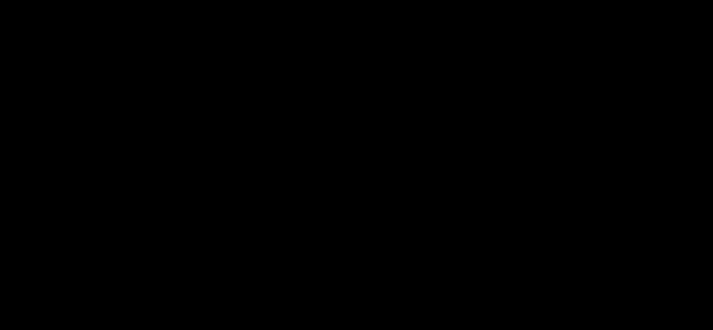
\includegraphics[width=\textwidth]{img/technology/sieve_pass_notpass.pdf}
\end{figure}
In the following, the dielectric particles are approximated by ellipsoids with three (generally different) half-axes $$\rho_a \leq \rho_b \leq \rho_c.$$ For the purpose of sieving, only the values of the shortest two half-axes, $\rho_a$ and $\rho_b$, decide whether the particle can pass through the sieve. The longest ellipsoid half-axis $\rho_c$ does not affect this, although it may influence the sieving speed. Therefore we can represent each three-dimensional particle with its projection on the smallest possible ellipse, which is described by its \textit{minor axis} $\equiv 2\rho_a$, and by its \textit{major axis} $\equiv 2\rho_b$ (which is, in fact, the \textit{medium axis} of the ellipsoid). For a given shape of a hole in a homogeneous flat sieve, it is easy to determine which values of minor and major ellipse axes allow a particle to pass through, and which not. For a square sieve such area in the parameter space forms a disk around the center of origin (Fig. \ref{fg_sieve_pass_notpass}a). It can be shown that when the sieve is diagonally stretched, forming a lozenge-shaped hole, the area of spheres allowed to pass transforms into an ellipse (Fig. \ref{fg_sieve_pass_notpass}b). When the hole shape is circular or elliptical, it is obvious that the area forms a part of a square or of a rectangle, respectively  (Fig. \ref{fg_sieve_pass_notpass}c,d).

The resonant frequency of a dielectric resonator depends on all three half-axes, $\rho_a \leq \rho_b \leq \rho_c$. In order to select a size fraction as narrow as possible, one has to use double sieving: the above sieve not allowing the fraction of particles too big, the bottom sieve removing the fraction of particles too small. This is where the anisotropic hole shapes become useful -- the bottom sieve can exclude also all oblong particles with the difference of $\rho_a \leq \rho_b$ too big. This effect is illustrated in Fig. \ref{fg_double_sieving}, which also presents a comparison between using more usual sieves with square/lozenge holes and the approach with a pair of sieves with micromachined square/elliptical holes. Obviously, the latter approach better discriminates between the \textit{shapes} of the ellipsoids. This advantage further gains on importance when the anisotropy of the sieve is low.

\begin{figure}[ht] \caption{Application of the effect from Fig. \ref{fg_sieve_pass_notpass} for separating a narrow fraction of ellipsoids between the sieves. Both combinations of \textbf{(a)} square-rectangular and \textbf{(b)} circular-elliptic sieves can be used, with the latter one promising better selectivity also in terms of the particle aspect ratio.} \label{fg_double_sieving} \centering 
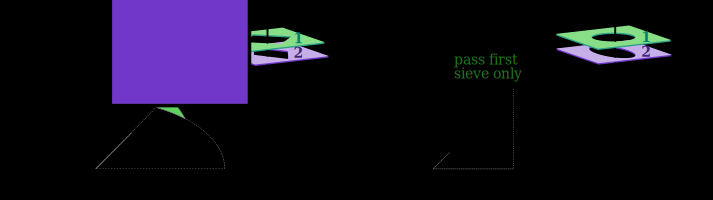
\includegraphics[width=\textwidth]{img/technology/sieve_double_sieving_fractions.pdf}
\end{figure}
It shall be noted that although we plotted a binary (pass/not pass) function in Figs. \ref{fg_sieve_pass_notpass} and \ref{fg_double_sieving}, the sieving speed continuously drops when the particle dimensions approach those of the sieve holes. 
%For any finite sieving time, this obviously affects the statistics of particles passing the sieve, favoring the average size to be lower for short sieving times.
However, this particular fraction of particles is exactly what one is interested in during the high-accuracy sieving. The process must therefore be run for a long enough time, of the order of days, and with as high a sieving speed as possible.
%}}}
\paragraph{First sieving apparatus}%{{{
%Finally, they were carefully sieved in many iterations, to select a size fraction as narrow as possible.
Employing the idea of anisotropic sieves from Fig. \ref{fg_double_sieving}a, the author assembled a first prototype based on nylon sieves, as depicted in Fig. \ref{fg_sieving1}. Two glass containers, 6 mm high and 11 mm in diameter, were cut on a lathe from a glass tube. On their bottom, the sieves were glued and carefully clipped. The side of the sieve holes was 60$\pm$5 $\upmu$m. 

The mesh was woven of nylon threads, so the bottom sieve could easily be stretched by ca. 20-25 \% in the diagonal direction.  The above sieve was kept isotropic. 

This  property however prove to be also detrimental for precise sieving, as the threads easily bent aside under only a small force, thus allowing oversized particles either to pass or to get stuck permanently and to block the sieve within few minutes. To help resolving the latter problem, two additional narrow glass rings were cut from the glass tube, supporting much coarser sieves with 150 $\upmu$m pitch glued on the bottom, to allow little spherical springs bounce beneath the sieves and to loosen the particles that got stuck in the holes. For the same purpose, 2mm plastic balls were added to the microsphere samples.  

A cover on top prevented the particles to jump out of the above container. The whole stack was carefully lowered into a test tube with a larger diameter, and vibrated by a tiny electric motor glued on the bottom.

\begin{figure} \caption{\textbf{(a)} Photograph and \textbf{(b)} scheme of the first sieving apparatus based on square-lozenge sieve pair, with a schematic out-of-scale illustration of its operation for an input of four different microspheres \textbf{(c)}}  \centering 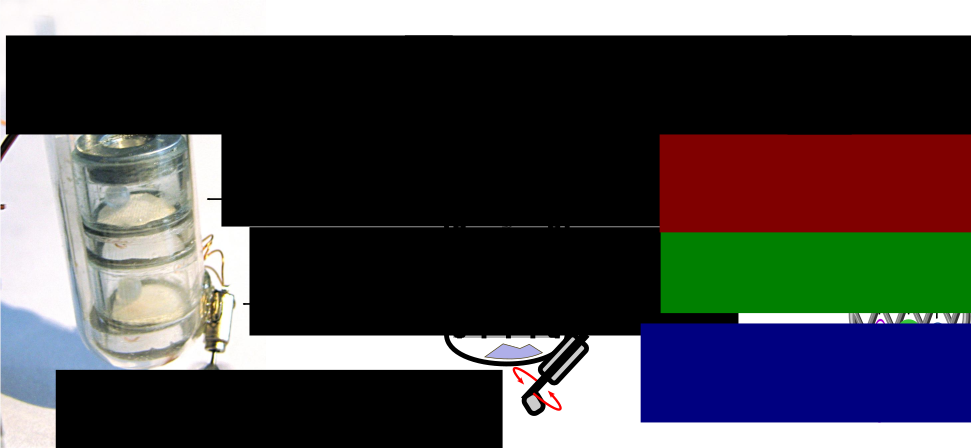
\includegraphics[width=12cm]{img/expe/sieving1.pdf} \label{fg_sieving1} \end{figure} 

%}}}
\paragraph{Second sieving apparatus}%{{{
\begin{figure}[ht] \caption{\textbf{(a)} A sketch of the acoustic sieving device, and \textbf{(b)} a photograph thereof} \label{fg_sieving2} \centering 
	\begin{overpic}[height=.4\textwidth]{img/technology/sieve2_sieving_scheme.pdf}  \put(-10,93) {\textbf{(a)}} \end{overpic}
	\begin{overpic}[height=.4\textwidth]{img/technology/sieving_m.pdf}              \put(1,85) {\textbf{(b)}} \end{overpic}
\end{figure}
The partially promising results and, more importantly, obvious deficiencies of the previous apparatus motivated the construction of a second one depicted in Fig. \ref{fg_sieving2}.
Different from any other sieving apparatus known to the author, this one made use of vertical acoustic waves for the movement of particles. It consisted of two coaxial glass tubes: The inner tube, with outer diameter of 13 mm, had a round metallic sieve glued to its bottom, and on its upper end it was covered by a small acoustic transducer. The outer tube (90 mm long, outer diameter 26 mm) surrounded the inner one and had a round bottom, where the particles were collected. 

The gaskets ensured that the whole apparatus was tightly closed, preventing both sieved particles and the sound from escaping. The brass ring with the transducer was fixed to a massive aluminum stand, and the rest of the structure was held by two accessible screws that allowed easy disassembling. 

The key advantages of this novel approach are the following:
\begin{enumerate}
 \item{The speed of sieving is expected to grow with the frequency at which the particles hit the sieve. The acoustic frequency of 1 kHz is roughly two orders of magnitude higher than in usual commercially available devices. Moreover, the spheres are  continuously stirred, so it is ensured that a layer of over-sized particles does not occupy the sieve.} 
 \item{The upward air pressure pulls out particles that got stuck in the sieve in every period of acoustic vibration. This resolves the major issue of clogging inherent for the previous prototype.} 
 \item{Avoiding macroscopic vibrating parts, except the membrane of a small acoustic transducer, allows the device to operate over multiple days with reduced risk of mechanical failure.}
 \end{enumerate}
The outer tube acted as an acoustic resonator, greatly enhancing the effect of the sound when tuned to resonance around 750-900 Hz. These frequencies obviously correspond to the fundamental acoustic resonance, as the corresponding quarter-wavelength is close to the 10 cm length of the outer tube.  The electrical input power of the sine wave feeding the device was in the order of 1 W.

%}}}
\paragraph{Sieving challenges}%{{{
A practical deficiency of this setup was that the upper opening of the transducer radiated relatively intense sound during operation. We resolved this potential issue by covering the whole apparatus by a robust glass bell jar.

With the acoustic power and frequency correctly adjusted, the particles formed a cloud 5--10 mm high. One difficulty arose from that the small particles tend to attach to the surface of glass or metal, probably due to electrostatic charges on their surface. While at an average particle radius $\rho = 50$ $\upmu$m this effect was rather marginal and transient, it took only few seconds of sieving for $\rho = 20$ $\upmu$m particles to immobilize permanently on any surface. It has however proven efficient to tap the upper brass ring, as the mechanical shock released most spheres and renewed the sieving process. To ensure unattended sieving for a timespan in order of days, we added a little motorized hammer with a timing circuit (Fig. \ref{fg_sieving2}a).

The amount of particles in one batch was limited to ca. 10--20 mm$^{3}$, otherwise the sieve would be covered with a layer too thick, which could not be efficiently lifted by the acoustic pressure.
This problem could however be slightly mitigated by tilting the apparatus. With a tilt of 5--10 degrees, the bulk of particles then accumulated near one side, leaving most of the sieve surface free for sieving the moving particles. Given the small amount of particles required for the terahertz spectroscopy measurements, it is however advisable to sort a batch in order of 1--3 mm$^{3}$.

%}}}
\section{Optical determination of microparticle statistics}
\paragraph{Image preparation} %{{{
An accurate characterisation of the particle statistics was necessary not only to assess the efficacy of sieving, but also to explain  possible differences between the measured terahertz spectra and the computed ones  on a quantitative basis. To obtain reliable statistics, thousands of particles needed to be evaluated, repeatedly for every sample. This, along with the small dimensions of particles, indicated that the most viable way to do so would be the optical microphotography with computer image processing automatically resolving each particle.

Computer \textit{granulometry}\index{granulometry}, identification and measurement of photographed particles from a digital image,
is a well-established technique. It is implemented in several advanced image processing programs, of which \textit{ImageJ} was selected \cite{abramoff2004image} since it is free of charge and allows its use for large batches of images through the use of macros. 

The transmission microphotographs were acquired either with the lowest magnification on a laboratory microscope, or with a portable microscopic digital camera on its highest magnification, yielding similar results.

The first processing step, applied at the somewhat blurred photographs, as shown in Fig. \ref{fg_sievingstats}a, was to establish the intermediate brightness level between the image's bright and dark areas, and apply a threshold so that the image was a binary function. Then the \textit{ImageJ}'s \textit{watershed} algorithm was applied to resolve two or more touching particles relatively reliably, and a particle outline was found. An example is depicted as cyan lines in Fig. \ref{fg_sievingstats}b. Finally, the particle outlines were approximated by best matching ellipses, and the major and minor axes of the ellipse were added into the statistics. 
\begin{figure}[ht] \caption{\textbf{(a)} A small section of a microphotograph of a pre-sieved sample before applying the described double-sieve method, \textbf{(b)} the corresponding identification of particles in ImageJ} \label{fg_sievingstats} \centering 
	\begin{overpic}[height=.30\textwidth]{img/technology/imagej_photo.pdf} \put(-9,72) {\textbf{(a)}} \end{overpic}\quad\quad
	\begin{overpic}[height=.30\textwidth]{img/technology/imagej_found.pdf} \put(-9,72) {\textbf{(b)}} \end{overpic}\quad\quad
\end{figure}
We complemented the \textit{ImageJ} macro with a Python script enabling us to process multiple photographs in a batch, and to plot the resulting histograms of the ellipse axes distribution. The script has also been published online \cite{dominec2014_imagej}. The scale for each batch of images had to be determined from a separate photograph of a ruler.

%}}}
\paragraph{Imprecision of the method} %{{{
An intrinsic deficiency of this method is that it was not possible to resolve the third dimension of particles. 
It can be however estimated that when % TiO$_{2}$ 
ellipsoidal particles were randomly sprinkled on the glass, they would lie mostly on their flat side -- i.e. their orientation would enable to measure the \textit{medium} $\rho_b$ and \textit{major} axes $\rho_c$ of the ellipsoid. This is in contrast with the process of sieving, as described above, where the particles were sorted according to their and \textit{minor} $\rho_a$ and \textit{medium} $\rho_b$ axes. 

This source of error is probably similarly important as another one, arising from rough shapes of the particles which could not always be well approximated by an ellipsoid. 
%\todo{add the previous and resulting statistics? the THz spectra should better go to the Results }
%}}}

\section{Laser cutting}
\paragraph{Fabrication of dielectric bars}%{{{
Dielectric or metallic structures can be made by cutting a thin polished slab of the given material. Electromagnetic waves with a frequency of  1~THz have a free-space wavelength of 0.3 mm. Periodic structures designed to operate in this range have their unit cells of a similar size or less, and their finest features are usually in the order of 10-20 $\upmu$m. 

The sample already shown in Fig. \ref{fg_STO_bar_rt} consisted of bars from strontium titanate (SrTiO$_{3}$) with a rectangular cross-section (see Fig. \ref{fg_STO_bar_geom}), where a structure with 10--30 $\upmu$m lateral bar dimensions was engraved into a thin slab of the dielectric of a similar thickness \cite{yahiaoui2011tunable}.

If the slab consists of a monocrystal or a ceramic, it is usually extremely brittle and also sensitive to breaking due to thermal stresses. Femtosecond laser cutting (or, micro-machining) is suitable for such a task because it delivers the energy so fast that most of the heated material evaporates before the heat can diffuse into the rest of the structure. 
The strontium titanate bars were fabricated by the \textit{Alphanov} facility in France.

%}}}
\paragraph{Fabrication of sieves and fishnets}%{{{
Femtosecond cutting of metallic sheets into two-dimensional meshes is relatively easy,   
compared to the dielectrics, 
and was implemented in our laboratory. To achieve the required precision, we used 20 or 30 $\upmu$m thick high-quality stainless steel foils. 

The femtosecond laser used was different from that serving as the femtosecond source for terahertz spectroscopy (Sect. \ref{sect_tdts}). A largely sufficient power was provided by the \textit{Spectra Physics Spitfire Ace} multipass titanium-sapphire amplifier, with 1 mJ of energy per impulse, duration of $\sim$50 fs, and 5 kHz repetition rate. Its output beam had to be attenuated to obtain finer cut at the expense of a slightly slower rate. The mechanical part consisted of two crossed \textit{Owis} stepper-motor controlled linear stages, and a fast mechanical shutter allowed us to control the beam with a sufficient resolution of ca. 100 ms. 
\begin{figure}[ht] \caption{\textbf{(a)} Laser cutting the steel foil with a moving holder for four samples, metal vapour ventilation, and the focusing lens. A bright plasma spot is visible at the focus. \textbf{(b)} The resulting sieves made from 30 $\mu$m stainless steel foil with 10 mm overall diameter.} \label{fg_microfab} \centering 
	\begin{overpic}[height=.35\textwidth]{img/technology/sieve2_drilling_m.pdf} \put(-8,82) {\textbf{(a)}} \end{overpic}\quad\quad
	\begin{overpic}[height=.35\textwidth]{img/technology/steel_sieve_on_paper.pdf} \put(-8,80) {\textbf{(b)}} \end{overpic}
\end{figure}

The 3 mm wide beam was focused by a lens with a focal length of 10 mm or 50 mm (Fig. \ref{fg_microfab}a). The tighter focusing lead to a better resolution, but had stricter requirements for accurate focusing of the beam. To facilitate the task of optimal focusing, we devised a focusing-collimating setup which used the fact that  the  steel foil reflected the light like from a point source only when it was exactly in the lens focus. Then the reflected light would be collimated again by the very same lens into a beam returning to the laser. 
%the reflection would not be collimated if the reflection occurred in front of the focal plane or behind it. 
A part of the beam energy reflected from the metal sheet was separated sideways by a skewed glass in front of the lens, so that one could finely align the lens seeking for the smallest spot diameter on a distant screen.

A compact stepper-motor controller of a custom design \cite{dominec2015_triostepper} facilitated to automate the sample movement by means of computer control operated by a Python script. The sequences of shutter opening, sample movement and shutter closing could be assembled into a program for fabrication of a whole mesh sample of ca. 10 mm diameter, which took about 30 minutes to finish. Multiple different meshes with different parameters could be cut out from one steel foil in a batch, without user interaction.

%}}}
\paragraph{Laser cutting issues}%{{{
The metal evaporated during the laser cutting immediately oxidises in the air. Although in total only few milligrams of the stainless steel foil were removed, the microscopic particles would pose a risk of damaging optical components. We built a miniature ventilation and filtering system out of a tube filled with cotton wool and fine synthetic fibres. After few meshes were cut, the cotton changed its colour from white to pale brown, indicating that at least a part of the particles were filtered out.

A greater challenge arose from thermal expansion of the foil. In order to fully utilise the valuable laser beam time, one would wish to set the cutting speed as high as possible. However, the speed of cutting was rather limited by the speed of stepper motors. The heat remaining in the steel foild was high enough to cause its thermal expansion and bending out of the plane of its holder. Even though the resulting displacement was less than 1 mm, the sheet moved significantly out of the beam focus. We assume this was the reason for slight variations between the hole sizes in Fig. \ref{fg_fishnet28_photo}. The effect would be diminished through slower cutting speed or by gluing the foil to a sacrificed rigid substrate.

Cutting the foil into free-standing wire array was however not successful since the resulting thin wires bent out of their original plane due to the thermal expansion. Their spacing was so uneven that no usable sample of wires was made.

%}}}
\paragraph{Difference between sieves and fishnets}%{{{
The meshes were made for two purposes -- either as sieves used in the second sieving apparatus described above, or as metamaterial samples known as \textit{fishnets}\index{metamaterial!fishnet!fabrication}, which are predicted to exhibit a negative index of refraction (see Sect. \ref{section_fishnet}). The difference between these applications is subtle; the meshes intended as sieves would surely exhibit a resonance in the terahertz range. 

The optimum  size range for the titanium dioxide spheres resonating around 1~THz is around 30--60 $\upmu$m, which determined the hole diameter of sieves. To maintain mechanical robustness, the periodicity in sieves was kept much larger than the hole diameter, usually 300$\times$300 $\upmu$m, and the thickness was chosen as 20 or 30 $\upmu$m.
The fishnets had the same periodicity as sieves, and the hole dimensions were chosen between 150 and 280 $\upmu$m. 
For cleaner cutting, a thinner stainless foil was used, with a thickness of 5 $\upmu$m.

% TODO
%To achieve the required precision of sieving, we fabricated the sieves by femtosecond laser drilling of 20--30 $\upmu$m thick stainless steel foil
%These sieves then were employed in a device that subjected the microsphere sample to acoustic vibrations, improving the speed of the demanding sieving process to acceptable level

%}}}



\chapter{Results}
\begin{flushright} \textit{``The purpose of computing is insight, not numbers.''} --- R. W. Hamming \end{flushright}
\label{chapter_results}
\section{Dielectric slab} \label{section_Dielectric slab}
\paragraph{Dispersion curves of a one-dimensional photonic crystal}%{{{
\begin{figure}[h] \caption{Dispersion curves \textbf{(a)} in free space with virtual periodicity $a$, \textbf{(b)} in dielectric layers with permittivity $\varepsilon = 12$ and 15 \% fill fraction. \\
Side plots show the electric field in $2\times 2$ unit cells, with dielectric outlined by thin black lines. The triplet of the electric $\E$ and magnetic $\HH$ fields and the wave vector $\KK$ for the incident wave is indicated in the lower left. The electric field is plotted as a blue-white-red color map.} \label{fg_1dbd} \centering 
	\begin{overpic}[width=.48\textwidth]{img/Slab_eps001_PWEM.pdf}  \put(1,96) {\textbf{(a)}} 
		\put(0,1){\includegraphics[width=.12\textwidth]{img/tripletKEH.pdf}}
	\end{overpic}
	\begin{overpic}[width=.48\textwidth]{img/Slab_eps012_d15.pdf}   \put(1,96) {\textbf{(b)}} \end{overpic}

\end{figure}
\begin{figure}[ht] \caption{Amplitude of \textbf{(a)} reflectance, \textbf{(b)} transmittance and \textbf{(c)} effective index of refraction $\Neff$ (real part solid, imaginary part dashed) for the dielectric slab of 15\% fill fraction in a 300 $\upmu$m unit cell, and varied permittivity of the dielectric $\epsrl \in \{4,12,20\}$} \label{fg_Slab_fillfraction015_epsilon_comparison} \centering \vspace{-3mm}
\begin{tabular}{r}
\begin{overpic}[width=0.95\textwidth]{img-meep/Slab_fillfraction015_epsilon_comparison_r.pdf} \put (-1,27) {\textbf{(a)}} \end{overpic}\vspace{-0.055\textwidth}\\
\begin{overpic}[width=0.95\textwidth]{img-meep/Slab_fillfraction015_epsilon_comparison_t.pdf} \put (-1,27) {\textbf{(b)}} \end{overpic}\vspace{-0.055\textwidth}\\
\begin{overpic}[width=0.96\textwidth]{img-meep/Slab_fillfraction015_epsilon_comparison_n.pdf} \put (-1,37) {\textbf{(c)}} \end{overpic}\vspace{-0.\textwidth}\\
\end{tabular}
\end{figure}
The one-dimensional photonic crystal (1-D PhC) has been investigated thoroughly in the previous century and found its major application in dielectric mirrors. It is the simplest representative of periodic structures, since  it exhibits only a subset of different phenomena that can be observed in other periodic structures. This is due to its continuous translational symmetry in the transverse direction that excludes all phenomena with a lower symmetry. 

Most importantly, no \textit{individual resonances} can occur in 1-D PhC; all interaction with the wave happens through partial reflection of the electromagnetic wave on the interfaces of the layers. The only type of the band gap observed is of the Bragg type.

Dispersion curves for two examples of one-dimensional photonic crystals were computed using PWEM and are shown in Fig. \ref{fg_1dbd}. 
Its left panel shows the folded dispersion curves for a plane wave propagating in vacuum on which we imposed virtual periodicity. To save space, the dispersion curves were plotted as \textit{folded}, but one can easily imagine how the curve unfolds into a linear dispersion of vacuum, known as the \textit{light line}. No scattering occurs for homogeneous vacuum, thus for any frequency $f$ exists a real wavenumber $k$ corresponding to a propagating wave and there are no band gaps of finite width. 

The right panel, Fig. \ref{fg_1dbd}b, is obtained by introducing periodic layers of dielectric with permittivity 12\% and 15\% filling fraction. The dielectric is outlined by thin black lines. Band gaps of nonzero width corespond to frequency ranges where the wave can not propagate through the structure. %TODO The first photonic band gap starts at the frequency, TODO at which exactly half wavelength matches the cell spacing, i.e. when $2\pi / K= a/2$ as is depicted in the subplot \textit{X1} of Fig. \ref{fg_1dbd}b. The next band starts at the same wavenumber $K$, but the wave now has higher frequency because in the subplot \textit{X2} of Fig. \ref{fg_1dbd}b it is shifted by half its period so that it maximizes the electric field energy that is localized in the areas of lower permittivity. Higher Bragg band gaps are formed by the same mechanism.

%}}}
\paragraph{Characteristics of Bragg-type band gaps}%{{{
The lower and upper edge of the photonic bands are located the high-symmetry points of the Brillouin zone, such as $\mathbf{\Gamma}$ or $\mathbf{X}$, which are equivalent to the wavenumber $K=m\pi/a$ for $m\in\mathbb{Z}$ in the one-dimensional case discussed. Whenever $K$ is in one of these points, the electric and magnetic fields are periodic in space, and can be easily visualized. The side plots of \ref{fg_1dbd} show the shapes of the electric field $E_x$ in the $(y,z)$ plane at respective frequencies of the band edges. To stress the fact that the field is periodic even in the $\mathbf{X}$ point, each of the side plots spans over 2$\times$2 unit cells. 

An important characteristic of each field pattern is the set of all points where the field amplitude remains zero over the evolution of time. Such sets will be denoted as \textit{nodal planes}, or also, more accurately, \textit{nodal surfaces}.

From all pairs of field plots that are connected by a photonic band (i.e. X2-$\Gamma2$, $\Gamma3$-X3 etc.), it can be deduced that one nodal plane dividing the unit cell in perpendicular orientation to the wave vector is always added when the frequency increases from the lower band edge to the upper one. This rule is more general and is satisfied by other structures, too. 

Typical for all Bragg band gaps (i.e. X1-X2, $\Gamma2$-$\Gamma3$, etc. in \ref{fg_1dbd}) is that between the lower and upper edges of each band gap, the phase increase across an unit cell does not change and thus $K$ remains constant, as does the number of the nodal planes. The field does change between these points, however, and the change is in the location of the \textit{nodal planes} such that the upper band-gap edge concentrates the field energy in mostly lower-permittivity regions. 

%}}}
\paragraph{Bragg and Fabry-Pérot resonances} %{{{
The \textit{Bragg condition} for the formation of a band gap in a periodic structure is that an integer number of half waves fits into the unit cell; i.e. that the phase difference $\phi_{1+2}$ of the wave along the unit cell is 
\begin{equation} \phi_{1+2} = d_1 n_1 \frac{\omega}{c} + d_2 n_2 \frac{\omega}{c} = \pi m, \text{ where } m\in \mathbb{Z}. \label{eq_braggcond}\end{equation}
where $d_{1,2}$ are the thicknesses and $n_{1,2}$ are the refractive indices of the two layers.

\begin{figure}[t] \caption{\textbf{(a)} Reflectance and \textbf{(b)} the imaginary part of the retrieved refractive index for a 1-D PhC, with filling fraction of 15~\% in a 300~$\mu$m unit cell, as a function of frequency and dielectric permittivity. On the right panel, the Fabry-Pérot condition from Eq. (\ref{eq_fpcond}) are marked by a thin dash-dotted line.} \label{fg_slab_eps_scan} \centering 
\begin{overpic}[width=0.48\textwidth]{img-meep/Slab_fillfraction015_epsilon_scan_r.pdf}\put(-1,80){\textbf{(a)}}\end{overpic}
\begin{overpic}[width=0.48\textwidth]{img-meep/Slab_fillfraction015_epsilon_scan_ni.pdf}\put(-1,80){\textbf{(b)}}\end{overpic}
\end{figure}

\begin{figure}[t] \caption{\textbf{(a)} Reflectance and \textbf{(b)} the imaginary part of the retrieved refractive index for a 1-D PhC, with relative dielectric permittivity of 4, as a function of frequency and filling fraction in a 300~$\mu$m unit cell} \label{fg_slab_ff_scan} \centering 
\begin{overpic}[width=0.48\textwidth]{img-meep/Slab_epsilon4_fillfraction_scan_r.pdf}\put(-1,80){\textbf{(a)}}\end{overpic} 
\begin{overpic}[width=0.48\textwidth]{img-meep/Slab_epsilon4_fillfraction_scan_ni.pdf}\put(-1,80){\textbf{(b)}}\end{overpic}
\end{figure}

The width of the band gap grows with the amplitude of the wave scattered from the unit cell. This amplitude however also depends on frequency and, in the case of a lossless dielectric slab, it vanishes whenever an integer number of the half-waves fits into either of the dielectric layers. For comparison with Eq. (\ref{eq_braggcond}), this condition is
\begin{equation} \phi_{1} = d_1 n_1 \frac{\omega}{c} = \pi m \text{\quad or \quad} \phi_{2} = d_2 n_2 \frac{\omega}{c} = \pi m, \text{ where } m\in \mathbb{Z}. \label{eq_fpcond}\end{equation}
Note that unlike the Bragg resonance, this effect can be observed even in a single isolated unit cell; in fact it is the well known \textit{Fabry-Pérot resonance}. 

The vicinity of a Fabry-Pérot resonance influences the position and width the neighbouring band gap, which can be found for different dielectric permittivity of the slab $\epsrl\in\{4,12,20\}$ in Fig. \ref{fg_Slab_fillfraction015_epsilon_comparison}.

As special case, the conditions for both Bragg and Fabry-Pérot resonances can be fulfilled simultaneously: a \textit{zero-width band gap} results and two photonic bands are adjacent to each other in the same way as they were in vacuum (c. f. Fig. \ref{fg_1dbd}a). In all cases of zero-width PBGs, the dispersion curves appear to approach the boundary of photonic bands (located in a high-symmetry point in the Brillouin zone) as lines with nonzero slope. In the analogy with the dispersion of electrons in a solid, this can be viewed as a \textit{Dirac point for photons-polaritons}, where the photons-polaritons have zero effective mass. The corresponding isofrequency contour may have a cusp in this point, rendering invalid even the generalised notion of the refractive index as elaborated in Section \label{indexofrefraction}.

An example of a structure that exhibits multiple zero-width band gaps is the 1-D PhC with equal optical thickness of both slabs ($d_1 n_1 = d_2 n_2$), but multiple such points exist when the dielectric permittivity or the dielectric filling fraction is changed, as depicted in Figs. \ref{fg_slab_eps_scan} and \ref{fg_slab_ff_scan}, respectively. These plots are also the simplest examples of the interplay between the individual resonance contained in the dielectric structure and the overall band-gap structure, a topic that will be discussed later in more detail.

%}}}
\paragraph{Local effective parameters of a 1-D PhC}%{{{
Employing the \textit{s-parameter} method based on FDTD simulation, as described in Chapter \ref{chapter_sparam}, one can obtain the scattering parameters (i.e. complex reflectance and transmittance) of a finite layer of the periodic structure, and eventually retrieve its local effective parameters: the index of refraction $\Neff(f)$, impedance $\Zeff(f)$, permittivity $\eeff(f)$ and permeability $\meff(f)$. The first one is plotted in Fig. \ref{fg_Slab_fillfraction015_epsilon_comparison}c, allowing to clearly identify the Bragg band gaps as regions where $\Neff'$ follows one of the Brillouin zone boundaries and $\Neff'' < 0$.

The question is to what extent the three remaining local parameters, $\Zeff$, $\eeff$ and $\meff$, have any physical meaning. As a generally accepted approach, they will be considered meaningful only for the long wavelength limit, i.e. $K$ close to the $\mathbb{\Gamma}$ where the effects of the spatial dispersion should be negligible. According to Fig. \ref{fg_Slab_fillfraction015_epsilon_comparison}c, this is for frequencies up to 100 or 200 GHz only. At any higher frequency, the retrieved wavenumber $K$ approaches the Brillouin zone boundary, marked by the dash-dotted line, and grows further.

In the low frequency limit of 1-D PhC, it was always observed that
\begin{enumerate}
\item{$\Zeff \approx 1/\Neff$, thus the effective permeability is $\meff = \sqrt{\Neff\Zeff} \approx 1$.} 
\item{The effective permittivity $\eeff$ is the weighted average of the constituent media, which determines the low-frequency limit for the refractive index:
	\begin{equation} \left.\Neff\right|_{K\ll 2\pi/a} =\left. \sqrt{\eeff}\right|_{K\ll 2\pi/a} \approx \sqrt{\frac{d_1 n_1^{2} + d_2 n_2^{2}}{d_1+d_2}} \label{eq_phc_eeff}\end{equation}
	}
\end{enumerate}
Notice in Fig. \ref{fg_Slab_fillfraction015_epsilon_comparison}c that $\Neff$ at higher frequencies converges towards its asymptotic value $\left.\Neff\right|_{K\rightarrow +\infty}$, which differs from the value obtained by Eq. (\ref{eq_phc_eeff}):
\begin{equation} \left.\Neff\right|_{K\rightarrow +\infty} \approx \frac{d_1 n_1 + d_2 n_2}{d_1+d_2} \label{eq_phc_neff}\end{equation}
The difference comes from that in the low-frequency limit, the electromagnetic energy concentration is higher in the areas of higher permittivity, whereas in the high-frequency limit it appears to be distributed evenly.
Note that with the correct branch retrieval procedure, the index of refraction never drops with frequency except for the photonic band gaps. Negative derivative of $\Neff(f)$ would otherwise imply that the group velocity would be higher than the phase velocity \cite{mikki2009electromagnetic}, which was never observed in 1-D PhC.

% TODO \paragraph{Transmission through a finite number of unit cells}
% illustrate the band-gap formation \cite{laktionov2008}
% (todo) find python script ----> compare TMM and FDTD for metallic slabs
% note the ripples inside the band-gap (for more cells)
% and note that the NRW effective parameters do not change; the method is exact here due to absence of evanescent fields, whose detrimental effect was described in -todo-
% finite planar structure with defect mode \cite{skoromets2013}
%\begin{figure} \caption{1red.pdf}  \includegraphics[width=3cm]{img/multilay_1red.pdf}
               %\caption{2gn.pdf}   \includegraphics[width=3cm]{img/multilay_2gn.pdf}
               %\caption{3bu.pdf}   \includegraphics[width=3cm]{img/multilay_3bu.pdf}
               %\caption{3grey.pdf} \includegraphics[width=3cm]{img/multilay_3grey.pdf}
               %\caption{4vio.pdf}  \includegraphics[width=3cm]{img/multilay_4vio.pdf} \end{figure} 

%}}}

\FloatBarrier %====================================================================================================
\section{Wire medium} \label{chap_wiremedium}
\paragraph{High-frequency behaviour}%{{{
The structure formed of a regular square lattice of conductive wires exhibits more interesting properties when the electric field is parallel to the wires, and this polarisation will be assumed in the following. The lattice of wires perpendicular to the electric field does not appreciably interact with the electromagnetic wave, until the wire thickness is of similar magnitude to their spacing; such a case is discussed in another Section \ref{section_eot}.

In the high-frequency part of the spectrum above the first photonic band, where more than a half wave fits into the unit cell, the layers of metallic rods can be approximated by thin scattering slabs from the previous section, since the high-frequency interaction of the wave can be described of photonic bands alternating with Bragg band gaps. In contrast with the dielectric PhC described above, no Fabry-Pérot resonances are observed and the scattering strength of the wire layers reduces monotonously with growing frequency.

\begin{figure}[ht] \caption{Amplitude of \textbf{(a)}  reflectance, \textbf{(b)} transmittance \textbf{(c)} effective index of refraction $\Neff$ and \textbf{(d)} effective permittivity $\eeff$ for the array of wires made of gold, depending on the wire radius $\rho_w \in \{1, 2, 4, 8, 16\}$ $\mu$m with a fixed unit cell size $a = 100$ $\mu$m and grid resolution of 1 $\mu$m. } \label{fg_Slab_fillfraction015_wireradius_scan} \centering \vspace{-3mm}
\begin{tabular}{r}
\begin{overpic}[width=0.85\textwidth]{img-meep/Wires_wireradiusscan_r.pdf} \put (-1,28) {\textbf{(a)}} \end{overpic}\vspace{-0.060\textwidth}\\ 
\begin{overpic}[width=0.85\textwidth]{img-meep/Wires_wireradiusscan_t.pdf} \put (-1,28) {\textbf{(b)}} \end{overpic}\vspace{-0.057\textwidth}\\
\begin{overpic}[width=0.86\textwidth]{img-meep/Wires_wireradiusscan_n.pdf} \put (-1,28) {\textbf{(c)}} \end{overpic}\vspace{-0.055\textwidth}\\
\begin{overpic}[width=0.86\textwidth]{img-meep/Wires_wireradiusscan_eps.pdf} \put (-1,28) {\textbf{(d)}} \end{overpic}\vspace{-0.030\textwidth}\\
\end{tabular}
\end{figure}

%}}}
\paragraph{Inductive behaviour at low-frequencies}%{{{
At low frequencies, in contrast, the interaction of the conductive wires with the electromagnetic wave becomes very strong and leads to completely different behaviour than that described above. For a frequency range from zero up to the \textit{effective plasma frequency} $f_p$, the array exhibits a band gap where $\Neff$ is pure imaginary and $k'\approx 0$. Therefore, in the low-frequency part of the spectrum, the local effective permittivity $\eeff$ is a physically meaningful quantity and follows the law typical of inductive media:
\begin{equation} \eeff(f) = 1 - \frac{f^{2}}{f_p^{2}}\label{eq_eeff_plasma}\end{equation}
Such a dependence of $\epsrl$ was already used in the Drude model in Eq. (\ref{eq_drude_eps}), and plotted in Fig. \ref{fg_Au_models}. Owing to this similarity to metals or plasma, wire arrays are denoted also as \textit{diluted metal} or \textit{artificial plasma} since 1950s \cite{merkel1973simulation, rotman1962plasma}, or as \textit{metallic delay dielectrics}, owing to the possibility to manipulate the phase and group velocities  \cite[p. 54]{brown1953artificial}.

The physical origin of $\eeff<0$ is different than in continuous media, where it is \textit{kinetic}, i.e., due to the effective mass of electrons. In contrast, the negative effective permittivity in wire arrays is the result of the \textit{self inductance} due to the magnetic field circulating around the conductor. 

Except for optical frequencies, $f_p$ does not substantially depend on the internal plasma frequency of the constituent metal, and such behaviour can be obtained even if wires are thought to be made of a perfect electric conductor (PEC).
The plasma frequency does, however, depend on the geometry described by two parameters, the wire radius $\rho_w$ and the unit cell size $a$. 

%}}}
\paragraph{Behaviour close to the effective plasma frequency}%{{{
The dependence of $f_p$ on the wire radius $\rho_w \in \{1, 2, 4, 8, 16\}$ $\upmu$m is illustrated by the spectra of reflectance, transmittance, refractive index and effective permittivity in Fig. \ref{fg_Slab_fillfraction015_wireradius_scan}. The effective plasma frequency $f_p$ can be easily determined as the point where $\eeff'(f)$ crosses zero  in the plot \ref{fg_Slab_fillfraction015_wireradius_scan}d. This coincides with the lower edge of the first photonic band in Fig. \ref{fg_Slab_fillfraction015_wireradius_scan}c. 

For the limit $f \rightarrow f_p+$, the \textit{phase velocity} $$c/n = c/\sqrt{\eeff(f)}$$ is proportional to $(f-f_p)^{-1/2}$ and thus very high. Conversely, the \textit{group velocity} $$v_g \approx 2\pi \mathrm{d}f/\mathrm{d}k = \mathrm{d}f/\mathrm{d}n$$ vanishes, being proportional to $(f-f_p)^{+1/2}$. The product of the phase and group velocities close to $f_p$ thus remains nearly constant $c^2$, which is a phenomenon commonly encountered also near the \textit{cut-off frequency} of metallic waveguides.

Exactly at $f=f_p$, the wire array medium can support the longitudinal oscillations of the charge, oriented parallel to the wires. They bear a close resemblance to plasmons in bulk media \cite{pendry1996extremely}.

Notice that for a single cell, the transition from negative to positive permittivity is not accompanied by any obvious spectral feature on the reflection/transmission plot. Except for the zero frequency, a layer of wires has always nonzero transmittance that increases with frequency. Independent of the wire conductivity, it is not possible to build a 100\% efficient wire polarizer.

%}}}
\begin{figure}[th]%{{{ fg_omegap_a
  \begin{minipage}[c]{0.69\textwidth}
\begin{overpic}[width=.98\textwidth]{img/EWire_plasmaF_spacingscan.pdf} \put (-1,60) {\textbf{(a)}} \end{overpic}\\
\begin{overpic}[width=\textwidth]{img/EWire_plasmaF_radiusscan.pdf}  \put (-1,58) {\textbf{(b)}} \end{overpic}\\
  \end{minipage}
  \begin{minipage}[c]{0.3\textwidth}
	  \caption{Comparison of numerical results (dots) and two analytic models (solid and dotted lines) for plasma frequency $f_p$ of a wire medium: \textbf{(a)} $f_p$ as a function of wire spacing for two different wire radii of 16 $\mu$m and 8 $\mu$m (red and blue curves/dots, respectively). The empty symbols correspond to significantly reduced FDTD resolution, added for comparison. \textbf{(b)} $f_p$ as a function of wire radius $\rho_w$.}\vfill \label{fg_omegap_a}
  \end{minipage}  
\end{figure} 

%}}}
\paragraph{Plasma frequency as a function of wire radius and unit cell size}%{{{
From Fig.  \ref{fg_Slab_fillfraction015_wireradius_scan}, it can be also deduced that $f_p$ is approximately proportional to the logarithm of $\rho_w$ if $\rho_w \ll a$. This is related to that a thicker wire should have slightly lower inductance per unit length (sometimes denoted as its \textit{self-inductance}). 

The effect of wire spacing $a$ is the opposite; with $a$ growing, the magnetic field has more space to circulate around the wir and $f_p$ reduces. 

Different analytic models were proposed for description of both effects. The early model by Pendry \textit{et al.} from 1996 \cite{pendry1996extremely} works well for thin wires: 
\begin{equation} f_p(\rho_w,a) \approx \sqrt{\frac{c^2}{2\pi \, a^2 \, \ln(\frac{a}{\rho_w})}}. \label{eq_fp_pendry}\end{equation}
Its refinement by Maslovski \textit{et al.} from 2003 \cite{maslovski2002wire} should be valid also for wires with relatively high fill fraction:
\begin{equation} f_p(\rho_w,a) \approx \sqrt{\frac{c^2}{2\pi \, a^2 \, \ln\left(\frac{a^2}{4\rho_w (a-\rho_w)}\right)}} \label{eq_fp_maslovski}\end{equation}

We ran two series of wire array simulations as a simple verification of both the FDTD algorithm against the mentioned analytic models. In the first series plotted in Fig. \ref{fg_omegap_a}a, we kept the wire radius constant $\rho_w = 16\,\upmu$m, or and changed the wire spacing $a$ (red points). We changed the radius to $\rho_w = 8\,\upmu$m in the second batch, marked by blue points. For comparison, we plot in the plasma frequency predicted by both analytic models from Eqs. (\ref{eq_fp_maslovski}, \ref{eq_fp_pendry}) as full and dotted lines with the color corresponding to the simulation parameters, respectively. 

To test the possible error introduced by the FDTD algorithm, we ran the simulation with different resolution - results with fine $1$ $\upmu$m grid are denoted by full circles, results with coarse $4$ $\upmu$m grid with empty squares overlaid relatively close to the respective high-resolution results.

In the second series of simulations plotted in Fig.  \ref{fg_omegap_a}b, we kept the spacing $a = 100$ $\upmu$m and changed the wire radius $r$. The analytic model and FDTD simulation give similar results (up to 5 \%) even for wire radii approaching roughly $a/4$. For thicker wires, the analytic model predicts higher plasma frequency than FDTD.  To conclude, the results of the model presented by Maslovski match the FDTD simulation with good accuracy for thin wires (where $r \lesssim a/5$). One possible application of the wire medium is in the construction of negative refractive index metamaterials, where a small negative real value of effective permittivity is desired.%%todo rewrite?

%}}}
%TODO \paragraph{Oblique propagation of the wave} % {{{
%ref Homogenisation of nonlocal media such as wires 
%\cite{capolino2009book}
%\cite{silveirinha2007metamaterial}
%\cite{belov2003strong}
%\cite{belov2002dispersion}
%\cite{silveirinha2005homogenization}
% nice refs  from 1950-1970: http://ece-research.unm.edu/summa/notes/SSN/note192.pdf

%}}}

\FloatBarrier %====================================================================================================
\section{Cut wires} \label{section_cutwires}
\paragraph{Individual resonances}%{{{
The low-frequency behaviour of the wire array is determined by the distributed inductance of the wires, which introduces negative effective permittivity up to the plasma frequency $f_p$. When the wires are cut in each unit cell, a three-dimensional periodic lattice of antennas is formed. Its important parameters are not only the inductance along each antenna, but also the capacitance across the gap between wires. In an analogy with a series LC (coil-capacitor) circuit, such antennas exhibit \textit{individual resonances} at some nonzero resonant frequency $0<f_r<f_p$. 

These resonances couple to the electromagnetic field by means of their electric dipole, and are thus denoted shortly as \textit{electric resonances}. This does not mean that no magnetic field is involved; in fact, the energy is exchanged between the resonant electric and magnetic fields each quarter-period. The situation partially changes with decreasing size of the particles. At optical frequencies, the energy is exchanged between the electric field and the kinetic energy of the electrons, while the magnetic field circulating around the metallic particle plays a minor role only. Such regime is known as \textit{plasmonic resonances} and was described by Mie in 1908 \cite{mie1908beitrage}.
% note the Bohren and Huffman implementation is in /home/filip/PhD/Misc/120400_analytic_Mie_scattering/

The spectra for the cut-wire structure are depicted in Fig. \ref{fg_CutWires_wireradius1u_cutwidth_comparison} for different cut distances $d_c$. Starting with the thinnest wire of $\rho_w = 2$ $\upmu$m (red curve), we can identify the individual resonance as the point close to  1200 GHz where even a single layer of unit cells reflects full wave amplitude and the transmittance drops to zero. Towards higher or lower frequencies from the resonance, the transmittance is relatively high.

%% TODO check if the spatial dispersion would be visible in the CDH plots
%% ...even here, with particles infinitesimally thin along the wave-vector, the spatial dispersion may be significant; arguably it was observed in 1970s by Merkel \cite{merkel1973simulation}, who remarks that
%% "It is interesting that the more exact expressions for the dielectric constant of the artificial dielectric, which considered both the effect of the capacitive dipole impedance and the dipole-dipole interaction, did not model the behavior of a Lorentzian plasma as well as the original simplified approach"
%% TODO note about plasmonic particles 
%}}}
\begin{figure}[h!] \caption{Amplitude of \textbf{(a)} reflectance, \textbf{(b)} transmittance, \textbf{(c)} effective index of refraction $\Neff = \Neff' + \ii \Neff''$ for the array of cut wires of radius $r_w = 1$ $\upmu$m made of gold, depending on cut distance $r_w\in \{2, 4, 8, 16, 32, 64\}$ $\upmu$m. The unit cell is cubic and its size is $a=100$ $\upmu$m.\\%{{{
In plot  \textbf{(d)}, the effective permittivity is illustrated for the thinnest cut distance $d_c = 2$ $\upmu$m. Although retrieved for the entire spectrum, the local effective parameters have physical meaning only when the wavelength is much larger than $a$, i.e. roughly from 0 to 500 GHz and from 1220 to 1280 GHz.} \label{fg_CutWires_wireradius1u_cutwidth_comparison} \centering \vspace{-3mm}
\begin{tabular}{r}
\begin{overpic}[width=0.85\textwidth]{img-meep/CutWires_wireradius1u_cutwidth_comparison_r.pdf} \put (-1,28) {\textbf{(a)}} \end{overpic}\vspace{-0.059\textwidth}\\
\begin{overpic}[width=0.85\textwidth]{img-meep/CutWires_wireradius1u_cutwidth_comparison_t.pdf} \put (-1,28) {\textbf{(b)}} \end{overpic}\vspace{-0.056\textwidth}\\
\begin{overpic}[width=0.86\textwidth]{img-meep/CutWires_wireradius1u_cutwidth_comparison_n.pdf}\put (-1,28) {\textbf{(c)}} \end{overpic}\vspace{-0.056\textwidth}\\
\begin{overpic}[width=0.85\textwidth]{img-meep/CutWires_wireradius1u_cutwidth_comparison_eps_r2.pdf} \put (-1,28) {\textbf{(d)}} \end{overpic}\vspace{-0.030\textwidth}\\
%\begin{overpic}[width=0.85\textwidth]{img-meep/CutWires_wireradius1u_cutwidth_comparison_ni.pdf}\put (-1,28) {\textbf{(d)}} \end{overpic}\vspace{-9.5mm}\\ \begin{overpic}[width=0.85\textwidth]{img-meep/CutWires_wireradius1u_cutwidth_comparison_eps_r2.pdf}\put (-1,28) {\textbf{(d)}} \end{overpic}\vspace{-0.030\textwidth}\\
\end{tabular}
\end{figure}
%}}}
\paragraph{Dispersion near an individual resonance}%{{{
Each individual resonance in a periodic structure forms a characteristic shape in the spectrum of effective index of refraction $\Neff(f)$. The following description will therefore be applicable to individual resonances in other resonant structures, as well. 

\begin{enumerate}
\item{At frequencies under the resonance, the electric dipole of the antenna oscillates in phase with the driving field and the resonance contributes the effective index of refraction $\Neff'(f)$. 
The spectrum of a periodic structure with an individual resonance differs from the spectrum of a homogeneous medium that was already described at the Lorentzian resonance curve in Fig. \ref{fg_oscillator_spectrum}b.
At some frequency $f \lesssim f_r$ below the resonance, the index of refraction $\Neff'(f)$ becomes high enough to join the closest Brillouin zone boundary which was above it. From this point up to the resonance frequency $f_r$, $\Neff(f)$ has nonzero imaginary part, and the medium exhibits a band gap.
} 
\item{Exactly at the resonance frequency, the interaction of the dipole with the field changes its sign, since above the resonance, the dipole starts to be oriented opposite to the driving field. 
The real part of the refractive index $\Neff'(f)$ ceases to follow one Brillouin zone and transitions to another Brillouin zone below it. In local media, individual resonances appears to be the only occasions for $\Neff'(f)$ to transition downwards.

The imaginary part of the refractive index, $\Neff''(f)$, is required by the Kramers-Kronig relations to exhibit a sharp peak at the resonance frequency, which is superposed over the broader background stemming from the band gap (see Fig. \ref{fg_CutWires_wireradius1u_cutwidth_comparison}c). 

The spectral width of the transition and peak is inversely proportional to the quality of the resonance. Whenever the structure is built from realistic materials with nonzero losses and its spatial dispersion can be neglected, $\Neff(f)$ is a continuous complex function.
} 
\item{The band gap continues up to some frequency $f > f_r$, where another photonic band begins between the same pair of Brillouin zones.  
} 
\end{enumerate}

The most important observation is that the resonance curve of $\Neff(f)$ in periodic structures is constrained between the closest two Brillouin zone boundaries, which can be understood as the "floor" and "ceiling" for the dispersion curve. Apparently a single individual resonance can not shift the transmittance phase by more than $\pi$ per each layer of unit cells. It can therefore introduce a band of imaginary $\Neff$, but for $\Neff$ to reach negative values, two resonances must be combined.

The impact of the individual resonances on the effective parameters $\eeff(f)$ and $\meff(f)$ will be discussed in the later section focused on the dielectric resonators. % TODO verify that I have done this

%}}}
\paragraph{Effects of the cut distance $d_c$}%{{{
An increase of the cut distance $d_c$ clearly increases the resonance frequency $f_c$. The reason is twofold: for a cut width small relative to the unit cell size, $d_c\ll a$, it is mostly due to reduced capacitive coupling between the cut wires; for cut width comparable or greater than the unit cell size, $d_c \gtrsim a$, reduction of the cut-wire inductance is more important.

Both the individual and Bragg-type resonances can be identified in the plot for different $d_c$ in Fig. \ref{fg_CutWires_wireradius1u_cutwidth_comparison}c. When $d_c \sim 16$  $\upmu$m, the individual resonance shifts above 1.5 THz and exchanges its order with the Bragg band gap. 
For $d_c \gtrsim 32$  $\upmu$m on, the individual resonances are similar to those for a $d_c\sim 2$ $\upmu$m, but are shifted by one Brillouin zone up.

%}}}
\begin{figure}[h!] \caption{Amplitude of \textbf{(a)} reflectance, \textbf{(b)} transmittance and \textbf{(c)} effective index of refraction $\Neff = \Neff' + \ii \Neff''$ for a metamaterial made of cut wires with radius $r_w$. Cut distance $d_c = 2$ $\mu$m, unit cell size $a=100$ $\mu$m.} \label{fg_CutWires_wirecut2um_wireradiusscan} \centering \vspace{-3mm} %{{{
\begin{tabular}{r}
\begin{overpic}[width=0.85\textwidth]{img-meep/CutWires_wirecut2um_wireradiusscan_r.pdf} \put (-1,28) {\textbf{(a)}} \end{overpic}\vspace{-0.060\textwidth}\\
\begin{overpic}[width=0.85\textwidth]{img-meep/CutWires_wirecut2um_wireradiusscan_t.pdf} \put (-1,28) {\textbf{(b)}} \end{overpic}\vspace{-0.060\textwidth}\\
\begin{overpic}[width=0.85\textwidth]{img-meep/CutWires_wirecut2um_wireradiusscan_n.pdf}\put (-1,28) {\textbf{(c)}} \end{overpic}\vspace{-0.030\textwidth}\\
\end{tabular}
\end{figure}
%}}}
\paragraph{Effects of the wire radius $\rho_w$}%{{{
The dependence of the resonance frequency $f_c$ on the wire radius, Fig. \ref{fg_CutWires_wirecut2um_wireradiusscan}, is somewhat more complicated: For thin enough wires in the $a=100$ $\upmu$m unit cell, the resonance frequency decreases with growing $\rho_w$, since the inter-wire capacity increases. 
For high enough $\rho_w$ an opposite mechanism prevails; $f_c(\rho_w)$ then starts growing as a result of reduction of the wire inductance.

While the change of the cut-wire radius $\rho_w$ relatively weakly reflects in the resonance frequency, its major impact is in the \textit{strength} of the individual resonance. Thick wires lead to stronger reflection out of resonances, which also translates into a wider band gap in Fig. \ref{fg_CutWires_wirecut2um_wireradiusscan}c.

%}}}

\paragraph{Experimental measurement of cut wire spectra}%{{{ 
Although we did not fabricate any cut-wire metamaterial, we used the terahertz time-domain spectroscopy to characterise cut-wire-on-silicon structures, one representative of which is photographed and sketched in Fig. \ref{fg_bousek}. The metallic wires were deposited on a silicon substrate, and at their ends, the silicon was doped to form diode-like transitions. 
\begin{figure}[ht] \caption{The sample of cut wires (pale yellow) on silicon (cyan) substrate. \textbf{(a)} Natural-colour photograph from an optical microscope,  \textbf{(b)} Geometry of the wires in micrometers. They were measured to be $6.5$ $\mu$m wide and $30$ $\mu$m long. The periodicity of cut-wires was $30\times 50$ $\mu$m.  } \label{fg_bousek} \centering 
\begin{overpic}[height=.40\textwidth]{img/bousek_splitwires_microphoto.pdf}  \put(0,78) {\textbf{(a)}} \end{overpic}\quad
\begin{overpic}[height=.40\textwidth]{img/bousek_splitwires_drawing.pdf}  \put(0,95) {\textbf{(b)}} 
		\put(55,0){\includegraphics[width=.12\textwidth]{img/tripletEKH.pdf}} % todo
\end{overpic}
\end{figure}

This kind of structure was designed to operate as a switch for the terahertz radiation, controlled by the current flowing along the orientation of the wires and modulating the conductivity of semiconductor transitions at the ends of each cut wire. For an unknown reason, the modulation of the terahertz signal was very weak, if any, in all of 7 supplied samples. The only observed kind of systematic modulation manifested as 2.2\% drop in amplitude of the transmitted terahertz waveform, and its temporal advance by no more than 18 fs. These values required to feed the structure with a maximum modulation signal, dissipating roughly 10 watt peak thermal power.

The sample presented above in Fig. \ref{fg_bousek}, though not applicable as a modulator, exhibits a clear electric resonance around 1550 GHz. This resonance is substantially broadened and weakened by the losses of the structure (red line in Fig. \ref{fg_bousekspectra}). A FDTD simulation of thin metallic stripes 30 $\upmu$m long and 6.5 $\upmu$m wide on a silicon substrate did not match the experimental spectra very well (green line in Fig. \ref{fg_bousekspectra}). 
%}}}

\begin{figure}[ht]  % fg_bousekspectra%{{{
	\caption{Comparison of experimental (red line) and simulated spectra (green and blue lines) for the cut-wire on silicon structure. The green line corresponds to the original geometry from Fig. \ref{fg_bousek}b; a better match with the experiment is obtained by changing the length of stripes from 30 to 40 $\mu$m (blue line).} \label{fg_bousekspectra} \centering 
\begin{overpic}[width=.85\textwidth]{img-expe/bousek.pdf}\end{overpic}
\end{figure}
Much better match was obtained by simple elongation of the conductive stripes to 40 $\upmu$m (blue line in Fig. \ref{fg_bousekspectra}). This may reflect the fact that the wires were surrounded by a highly doped, conductive zones of silicon.
Although not taking into account the dissipative losses, such a simulation correctly identifies the resonance freqeuncy of the stripes. It also, at least quantitatively, matches the asymmetric spectral shape, which is caused by the onset of diffraction into the silicon substrate at $f_c = c/(50\;$ $\upmu$m$)/N_{\text{Si}} \approx 1730$ GHz. 

The presented simulations were not optimized for the dissipative losses in silicon, which could be modeled with more detailed knowledge of the structure preparation.

%}}}

%     \FloatBarrier %====================================================================================================
%     \section{Electric resonators} \label{section_esrr} % references to -> % note about plasmonic particles 
%     \paragraph{Comparison of spectra to the cut wires}%{{{
%     From Figs. \ref{fg_CutWires_wirecut2um_wireradiusscan} and \ref{fg_CutWires_wireradius1u_cutwidth_comparison} it follows that for any practically attainable geometry, the frequency of the first individual resonance in cut-wire arrays is always relatively close to the first Bragg band gap. 
%     
%     A viable way to shift the resonance frequency much lower, without changing the unit cell size nor resorting to submicrometre cut distances, is to replace straight wire antennas by \textit{electric split-ring resonators}, % TODO cite 
%     depicted in Fig. \ref{fg_eSRR}.
%}}}

\FloatBarrier %====================================================================================================
\section{Split-ring resonator} \label{section_srr} % references to -> 
\paragraph{Resonances with magnetic dipole moment}%{{{
The fundamental resonance in a cut wire has the electric dipole moment only. The resonant magnetic field circulates around the wire and due to its rotational symmetry along the $x$-axis, the magnetic dipole moment is zero. Other structures can support resonances of lower symmetry with regards to the $x$-axis, thus having a magnetic dipole moment.

One of the simplest examples is formed by bending the wire into a "C"-shaped \textit{split-ring resonator} (SRR). To reduce the resonant frequency, capacitor pads can be added to the cut, as shown in Fig. \ref{fg_SRR_types}a. The first resonance in its spectrum has a dominant magnetic dipole moment, and will be denoted simply as a \textit{magnetic resonance}. The electric current flows through the wire along a circular path, while the magnetic field has a toroidal shape around the wire.   

The very concept of SRR is at least as old as the Hertz's experiments with the spark-gap transmitter from 1880s.
As described in the historical review of Ref. \cite[pp. 120--126]{solymar2009waves}, first SRR arrays were built in early 1980s with the aim to build an effective medium with highly lossy complex permeability; a decade later asymmetric SRRs were used to achieve strong bianisotropy. Many publications cite Refs. \cite{pendry1999magnetism,pendry2000negative} from Pentdry et al. as the first application of SRR array for achieving negative effective permeability and index of refraction, respectively. Since then, the number of SRR-related publications has grown rapidly. 
\label{negn_srr}

\begin{figure}[h] \caption{Variants of the split-ring resonators, viewed from the side perpendicular to the magnetic field: \textbf{(a)} classical SRR, \textbf{(b)} symmetric SRR with two splits, \textbf{(c)} one of the designs of an electric SRRs having a central bar, \textbf{(d)} a similar structure where the central bar was split by a capacitor with pad radius $\rho_c$, allowing to tune the electric resonance} \label{fg_SRR_types} \centering 
\begin{overpic}[height=0.25\textwidth]{img/drawing_SRRpad.pdf}\put (1,80) {\textbf{(a)}}\end{overpic}\qquad
\begin{overpic}[height=0.25\textwidth]{img/drawing_sSRRpad.pdf}\put (-2,80) {\textbf{(b)}}
		\put(110,30){\includegraphics[width=.12\textwidth]{img/tripletEHK.pdf}}
\end{overpic}\qquad
\end{figure}

%}}}
\paragraph{Symmetry of the split-ring}%{{{
The orientation of the splitting in the SRR determines the possible coupling between its electric and magnetic dipoles. In particular, when the splitting is on the front or rear side of the ring relative to the  direction of wave propagation, the predominantly magnetic resonance creates also a weak electric dipole, leading to the optical activity.

Reduced symmetry with regards to the wave propagation may even break the homogenisation based on scattering parameters retrieval, as this procedure assumes that the structure is symmetric, i.e., its reflectance is equal from both sides. Asymmetric structures therefore have properties that can not be matched by any (reciprocal) homogeneous medium. 

The symmetry is restored again by considering a \textit{symmetric split ring resonator} (sSRR), depicted in Fig. \ref{fg_SRR_types}b, which has two splittings at opposing position on the ring. 
% A. Andryieuski, C. Menzel, C. Rockstuhl, R. Malureanu, and A.V. Lavrinenko, The split cube in a cage: %bulk negative-index material for infrared applications, Journal of Optics A: Pure and Applied Optics,
%vol. 11, p. 114010, 2009.
This is documented by the results in \ref{fg_SRR_principles}. The SRR with a single splitting is represented by red lines; while its magnitude of reflectance and transmittance in Fig. \ref{fg_SRR_principles}a,b appear similar to these of a cut wire, the computation of the refractive index yields a spectrum (Fig. \ref{fg_SRR_principles}c) which has no reasonable interpretation near the resonance at 500 GHz and above it. 

The symmetric resonator is represented by green curves. In Fig. \ref{fg_SRR_principles}c, the refractive index follows a resonance pattern that was already described on the example of the cut wires: the curve grows up to the upper Brillouin zone boundary, follows it for a span of frequencies, drops to the Brillouin zone boundary below, follows it again and then a next band starts. 

At higher frequencies, outside the range of Fig. \ref{fg_SRR_principles}, the SRR exhibits also the electric resonance where the current flows symmetrically along both its arms. It is assumed that any structure should support infinite number of resonances, of which only the lowest few are usually of any interest.
%}}}
\paragraph{Antiresonances in local effective parameters}%{{{
In the case of symmetric split-ring resonators, the first resonance possesses only the magnetic dipole moment, as follows from the symmetry of the resonant fields. This fact reflects in a strong resonant behaviour of the permeability $\meff(f)$ (green curve in Fig. \ref{fg_SRR_principles}e, between 600 and 700 GHz). 

The permittivity spectrum $\eeff(f)$ is, however, also affected by the magnetic dipole resonance  (Fig. \ref{fg_SRR_principles}d). The impact of the magnetic resonance on $\eeff(f)$ is several times weaker than on $\meff(f)$, and more importantly, it has an opposite sign: The real part of $\eeff'(f)$ is reduced at frequencies below the resonance, and increased above it. Simultaneously, the sign of the imaginary part $\eeff''(f)$ would imply amplification of the electric field oscillating around 650 GHz, which is impossible in a structure composed of lossy materials only. This feature in the spectrum is sometimes described as an \textit{antiresonance} and has incited much discussion in the literature \cite{koschny2003resonant, wallen2011anti}. 
%}}}
\paragraph{Physical relevance of effective parameters in their local approximation}%{{{
We believe that the influence of a magnetic resonance on $\eeff(f)$, or conversely, of an electric resonance of $\meff(f)$, is a mere artifact of approximating a strongly nonlocal structure with a concept of local effective parameters. It can be shown antiresonances become stronger at higher frequencies, as the wavelength $2\pi/K$ becomes similar to the unit cell size $a$. 
In Ref. \cite{wallen2011anti}, it is argued that % against this interpretation with
\begin{displayquote}
\textit{the periodicity cannot \ldots be the only explanation since qualitatively similar antiresonances have been reported using the measured data for a disordered high permittivity composite.}
\end{displayquote}
The true origin of antiresonances and other deviations of $\eeff(f)$ and $\meff(f)$ from the Lorentzian resonance curve can however be attributed to the presence of photonic band gaps and nonlocal response of the structure. These effects are, to some extent, maintained also under randomizing the unit cell positions \cite{peng2007},   
thus there is probably no need to seek for another explanation. %%TODO rewiew, rewrite?
% \cite{alu2010} "Restoring the physical meaning of MM constitutive parameters"

%An elaborate comparison of resonant metallic structures, with clear effect of adding the wire to the transmission spectra, can be found e.g. in Ref. \cite{koschny2004effective}.

%Ref. \cite{li2009determination} contains typical complex-valued spectra of $\eeff$ and $\meff$ for a SRR and SRR-Wire
% different orientations - some leading to chirality i.e. linear dependence of f(K)
% when not failing due to chirality, s-param yields beautifully similar results to our simulations!
% "CMM = Composite MetaMaterial"
%}}}
\paragraph{Comparison of the s-parameters method and CDH}%{{{
With local effective parameters $\eeff(f)$ and $\meff(f)$ appearing to lose their physical meaning in a frequency range near a resonance, a question remains to what extent the dispersion curves, or equivalently, the spectrum of effective index of refraction $\Neff(f)$ is applicable. While the Bloch theorem in Eq. (\ref{eq_bloch}) suggests that the dispersion curves for the Bloch wavevector $\KK$ can be determined for any periodic structure, the s-parameter method might return invalid values.

Dispersion curves obtained by the s-parameters method and by the current-driven homogenisation (CDH) are compared in Fig. \ref{fg_cdh5}. Although these methods are fundamentally different, their results overlap, and thus one can assume that the array of symmetric split-ring resonators can be treated as homogeneous with well-defined index of refraction $\Neff(f)$ for the Bloch wave over the whole spectrum. Its local effective parameters $\eeff(f)$ and $\meff(f)$, however, seem to have no useful physical interpretation near the resonances, where the Bloch wavelength is similar to the unit cell size. They remain useful farther from the resonance, though. % todo perhaps add some particular frequency ranges from the Fig.

%}}}
\paragraph{Variants of split-ring resonators}%{{{
\begin{figure}[t] \caption{Other variants of split-ring resonators: \textbf{(a)} double SRR, \textbf{(b)} symmetric version thereof, \textbf{(c)} double SRR with cross-connection between the inner and outer rings, \textbf{(d)} illustration of a square variant of the double SRR, \textbf{(e)} the "omega" structure aimed to introduce $\Neff'<0$, \textbf{(f)} the cut-wire pair} \label{fg_SRRothers} \centering 
\begin{overpic}[height=0.22\textwidth]{img/drawing_dSRRpad.pdf}    \put (1,81) {\textbf{(a)}}\end{overpic}\quad
\begin{overpic}[height=0.22\textwidth]{img/drawing_dsSRRpad.pdf}   \put (1,81) {\textbf{(b)}}\end{overpic}\quad
\begin{overpic}[height=0.22\textwidth]{img/drawing_dSRRcrossed.pdf}\put (1,81) {\textbf{(c)}}\end{overpic}\\
\begin{overpic}[height=0.22\textwidth]{img/drawing_dSRRsquare.pdf} \put (-7,81) {\textbf{(d)}}\end{overpic}\quad
\begin{overpic}[height=0.22\textwidth]{img/drawing_SRRomega.pdf} \put (-6,81) {\textbf{(e)}}\end{overpic}\quad
\begin{overpic}[height=0.22\textwidth]{img/drawing_strippair.pdf} \put (1,81) {\textbf{(f)}}
		\put(100,30){\includegraphics[width=.12\textwidth]{img/tripletEHK.pdf}}
\end{overpic}\quad
\end{figure}
Diverse metamaterial designs based on the SRR principle were developed.
Many SRR designs involve a smaller ring nested inside the original one, as shown in Fig. \ref{fg_SRRothers}a,b in the asymmetric and symmetric variants. The long narrow gap between the inner and outer split ring enhances their capacitive coupling. This way, the frequency of the magnetic resonance can be reduced without increase of the overall SRR dimensions. Such designs usually do not need capacitor pads, and can be made by etching or microlitography. 

A modification of this \textit{double split-ring} design includes cross-connection between the inner and outer conductors as in Fig. \ref{fg_SRRothers}c; this version also breaks mirror symmetry. 

The square "ring" resonator (Fig. \ref{fg_SRRothers}d) is also widely used, without any substantial difference from the round SRR.

The \textit{omega structure} was designed to emulate the operation of a SRR and a wire simultaneously, by interconnecting the ends of a SRR along the $x$-axis (Fig. \ref{fg_SRRothers}e).

All SRR structures in Fig. \ref{fg_SRRothers} can be made flat in the plane perpendicular to the magnetic field, which facilitates their fabrication. At terahertz and higher frequencies, using a thin metal film should not be much detrimental to the SRR conductivity, since the skin depth caused by eddy currents is often submicroscopic \cite{gibbons2010scalable}.

On the contrary, a similar way of operation is achieved by structures infinite in the direction of the magnetic field. This allows to fabricate magnetic resonators by rolling stripes of a semi-metallised plastic foil, producing a \textit{swiss-roll} metamaterial \cite{gibbons2010scalable}, or by partially sputter-coating a polymer fibre by metal \cite{wang2011fiber}. Such structures however seem to exhibit relatively high losses when applied above the microwave range.

Metallic \textit{cut-wire pair}, or also \textit{strip pair}, metamaterial depicted in Fig. \ref{fg_SRRothers}f, was designed for operation in the infrared or optical range. It can be understood as a split-ring resonator flattened along the direction of the wave vector. The geometry is tuned so that the electric and magnetic resonances overlap.	

%}}}
\paragraph{SRR in a wire array} %{{{
The analysis of the wire array has shown that at low frequencies, its effective permittivity is physically valid and has a negative value. Likewise, the symmetric SRR has a region in the spectrum above its magnetic resonance where its effective permeability is negative, too.

A synthesis of these two structures yields a region of negative index of refraction, probably the first \cite{pendry2000negative} and most prominent metamaterial design to achieve this. The effect of combining structures that interact exclusively with magnetic and electric field is discussed in Ref. \cite{koschny2004effective} in more detail.

The resulting effective parameters are represented by the blue line in Fig. \ref{fg_SRR_principles}. Its spectrum of the effective index of refraction resembles that of the wire array up to 630 GHz, where it drops by one Brillouin zone down at the resonant frequency.
As a general rule observed in all correctly retrieved spectra, a single individual resonance always causes $\Neff'(f)$ to drop from one Brillouin zone boundary to another. 

Notice that the magnetic resonance causes a drop in $\Neff'(f)$ even without the wire array (green curve in Fig. \ref{fg_SRR_principles}c), but in such a case it happens between the first Brillouin zone boundary and zero. Without wires, $\Neff'$ does not reach negative values.

By contrast, a magnetic resonance in the combined SRR-wire structure introduces a narrow region, still within the photonic band gap, where 
\begin{equation} \Neff(f) = -\frac{c}{2 a f}, \label{eq_BZN2}\end{equation}
with $a$ being the unit cell size.	

The photonic band spanning from 635 to 670 GHz thus has $\Neff'<0$, but the effective permittivity and permeability can be attributed with physical meaning only when $\Neff'$ comes closer to zero, roughly from 650 to 670 GHz. They are correctly retrieved as both negative, as can be indeed seen from in Figs. \ref{fg_SRR_principles}d,e (blue lines).

%}}}
\paragraph{Fano resonance} %{{{
The spectrum of reflectance magnitude $|r(f)|$ for the sSRR-wire structure (blue line in Fig. \ref{fg_SRR_principles}a) has a relatively complex shape -- starting from a high reflectance introduced by the wire array, it grows below the magnetic resonance, then it drops to zero around 660 GHz, and it grows until its local maximum on 750 GHz is reached.

It differs significantly from the arguably simpler spectrum of the cut wires (Figs. \ref{fg_CutWires_wireradius1u_cutwidth_comparison}a and \ref{fg_CutWires_wirecut2um_wireradiusscan}a), where the resonance was accompanied by a single peak in reflectance. Since the structures have negligible lossess, complementary observations can be made with the transmission spectrum.

The reason is in that with the sSRR-wire structure, $|r(f)|$ is a linear superposition of the wave scattered by the interaction of the structure with the electric field, which has relatively large amplitude $r_{1}(f)$ over broad spectral range, and another wave $r_{2}(f)$ scattered by the magnetic dipole which is prominent only close to the magnetic resonance, between 550 and 750 GHz.

Both scattered components, $r_1(f)$ and $r_2(f)$, are complex functions. The phase of a wave scattered by a resonant element differs almost by $\pi$ for $f$ below and above the resonance. The impact on the plot of the overall reflectance is in a change from a constructive to destructive interference between the two components. 

Such typical spectral features, observed whenever a narrower resonance overlaps with another broader one, are known as \textit{Fano resonances}, and can be found on most following plots of $|r(f)|$ or $|t(f)|$. On the contrary, when the Fano lineshape is missing in the spectrum of a structure that obviously possesses a magnetic dipole, it suggests the homogenization would have failed (see, e.g., the spectra of the asymmetric SRR in \ref{fg_SRR_principles}).  

%}}}
\begin{figure}[t] \caption{Split-ring resonator: %{{{
		amplitude of \textbf{(a)} reflectance, \textbf{(b)} transmittance, \textbf{(c)} effective index of refraction,  \textbf{(d)} effective permittivity $\eeff$ and \textbf{(e)} effective permeability $\meff$  .   %% todo check params comment=sSRR with wire_resolution=2.000e-06_capacitorr=1.000e-05_splitting=4.000e-06_wirethick=4.000e-06_splitting2=4.000e-06_radius=3.000e-05_simtime=2.000e-10
Outer ring radius $\rho = 30$ $\mu$m, conductor cross-section $\Delta\rho = 6$ $\mu$m, unit cell size $a=100$ $\mu$m. \\
Comparison of the more familiar standard SRR (split width $d=4$ $\mu$m) with its symmetric variant sSRR (double split width $d=2$ $\mu$m) and the same sSRR with wire grid added. The dispersion curves nor effective parameters for the asymmetric SRR could not be determined by the scattering parameters method. } \label{fg_SRR_principles} \centering \vspace{-3mm} 
\begin{tabular}{r}
\begin{overpic}[width=0.85\textwidth]{img-meep/SRR_principles_r.pdf} \put (-1,28) {\textbf{(a)}} \end{overpic}\vspace{-0.060\textwidth}\\
\begin{overpic}[width=0.85\textwidth]{img-meep/SRR_principles_t.pdf} \put (-1,28) {\textbf{(b)}} \end{overpic}\vspace{-0.060\textwidth}\\
\begin{overpic}[width=0.85\textwidth]{img-meep/SRR_principles_n.pdf}\put (-1,28) {\textbf{(c)}} \end{overpic}\vspace{-0.060\textwidth}\\
\begin{overpic}[width=0.85\textwidth]{img-meep/SRR_principles_eps.pdf}\put (-1,28) {\textbf{(d)}} \end{overpic}\vspace{-0.060\textwidth}\\
\begin{overpic}[width=0.85\textwidth]{img-meep/SRR_principles_mu.pdf}\put (-1,28) {\textbf{(e)}} \end{overpic}\vspace{-0.030\textwidth}\\
\end{tabular}
\end{figure}
\begin{figure}[h] \caption{Current-driven homogenization results, shown as bubbles,  indicating the dispersion curves 
	for \textbf{(a)} a symmetric split-ring resonator and \textbf{(b)} the same with a wire mesh. The results of the scattering-parameters method are overlayed as green lines; these show the same data as the green and blue solid lines from Fig. \ref{fg_SRR_principles}c. In the right panel, the negative-index range of frequencies between 630 and 670 GHz was mirrored against the $K=0$ vertical axis and plotted by a dashed green line.} \label{fg_cdh5} \centering  % todo add params SRRArray_comment=symmetric SRR_simtime=2.000e-10_wirethick=0.000e+00_splitting2=1.600e-05_radius=3.000e-05_model=SRRArray.pdf
	% TODO recalculate and update
	\vspace{.1\textwidth}
	\begin{overpic}[width=.48\textwidth]{img-cdh/cdh_sSRR.pdf}  
	\put(1,96) {\textbf{(a)}} 
	\put(18,100){
\includegraphics[width=.1\textwidth]{img/drawing_sSRRpad.pdf}}
	\put(31,105){sSRR}
	\end{overpic}
	\begin{overpic}[width=.48\textwidth]{img-cdh/cdh_sSRR_wire.pdf}  
	\put(16,100){\includegraphics[width=.1\textwidth]{img/drawing_sSRRpad_wire.pdf}}
	\put(29,105){sSRR + wire}
	\put(1,96) {\textbf{(b)}} 
	\end{overpic}
\end{figure}

% todo possibly recalculate CDH for the SRR as in \ref{fg_SRR_principles}
%\begin{figure}[h] \caption{Current-driven homogenization results for the split-ring resonator \textbf{(a)} without the wire mesh and \textbf{(b)} with the wire mesh. 
	%} \label{fg_cdh4} \centering 
	%\begin{overpic}[width=.48\textwidth]{img-cdh/cdh_SRR.pdf}  \put(1,96) {\textbf{(a)}} \end{overpic}
	%\begin{overpic}[width=.48\textwidth]{img-cdh/cdh_SRRWire.pdf}  \put(1,96) {\textbf{(b)}} \end{overpic}
%\end{figure}
%}}}


\FloatBarrier %====================================================================================================
\section{Combined electric and magnetic resonator} \label{section_srr} % references to -> 
\paragraph{Effect of the central bar in SRR}%{{{
The fundamental resonance of a split-ring resonator (SRR) is the magnetic one, where the current circulates around its circumference. When one adds a central bar parallel to the electric field and the $x$-axis, as in Fig. \ref{fg_SRR_elmag}a, the frequency of the magnetic resonance does not change significantly. The reason comes from the symmetry thereof, which stipulates that that zero net current flows through the central bar. 

However, a new electric resonance (Fig. \ref{fg_emcSRR_resonances}b) is introduced by adding the bar, characteristic by that the current conducted by the central bar is antiparallel to the current conducted by both SRR arms. The corresponding frequency is lower compared to the original parallel electric resonance (Fig. \ref{fg_emcSRR_resonances}c), and similar to the frequency of the magnetic resonance (Fig. \ref{fg_emcSRR_resonances}a).  
\begin{figure}[h] \caption{\textbf{(a)} A modification of a split-ring resonator with a central bar, \textbf{(b)} a similar structure where the central bar was split by a capacitor with pad radius $\rho_c$, allowing to tune the antiparallel electric resonance} \label{fg_SRR_elmag} \centering 
\begin{overpic}[height=0.25\textwidth]{img/drawing_eSRRpad.pdf}\put (1,80) {\textbf{(a)}}\end{overpic}\quad\quad\quad
\begin{overpic}[height=0.25\textwidth]{img/drawing_emcSRRpad_sizes.pdf}\put (1,80) {\textbf{(b)}}\end{overpic}
\end{figure}
\begin{figure}[b] \caption{Three low-frequency resonances in the combined SRR: \textbf{(a)} magnetic resonance, \textbf{(b)} antiparallel electric resonance, \textbf{(c)} parallel electric resonance.\\ The actual order of the first two resonances in the spectrum is determined by the inner capacitor radius $\rho_c$ or other parameters of the structure.} \label{fg_emcSRR_resonances} \centering 
\begin{overpic}[height=0.22\textwidth]{img/drawing_emcSRRpad_resM.pdf}\put (1,81) {\textbf{(a)}}\end{overpic}\quad
\begin{overpic}[height=0.22\textwidth]{img/drawing_emcSRRpad_resE2.pdf}\put (1,81) {\textbf{(b)}}\end{overpic}\quad
\begin{overpic}[height=0.22\textwidth]{img/drawing_emcSRRpad_resE2b.pdf}\put (5,54) {\textbf{(c)}}
		\put(100,10){\includegraphics[width=.1\textwidth]{img/tripletEHK.pdf}}
\end{overpic}\qquad\quad
\end{figure}

%}}}
\paragraph{Tuning the frequency of the antiparallel electric resonance}%{{{
The spectra of the cut wires (Fig. \ref{fg_CutWires_wireradius1u_cutwidth_comparison}) suggest that each electric resonance, if not preceded by a Bragg band gap or excessively lossy, introduces a region in spectrum where the local effective permittivity has a physically meaningful and negative value. Under the same condition in Fig. \ref{fg_SRR_principles}, the magnetic resonance introduces a region of $\meff(f) < 0$.
\begin{figure}[t] \caption{Combined electric-magnetic resonator: amplitude of \textbf{(a)} reflectance, \textbf{(b)} transmittance and \textbf{(c)} effective index of refraction $\Neff = \Neff' + \ii \Neff''$.  
% todo check the structure parameters
%Outer ring radius $\rho = 30$ $\mu$m, conductor cross-section $\Delta\rho = 6$ $\mu$m, unit cell size $a=100$ $\mu$m. \\
%Comparison of the more familiar standard SRR (split width $d=4$ $\mu$m) with a symmetric SRR (double split width $d=2$ $\mu$m) and the same symmetric SRR with wire grid added.  The effective parameters for the asymmetric SRR could not be determined by the scattering parameters method.  %TODO params and comment 
The frequency of the electric resonance is influenced by the radius $\rho_c$ of the capacitor on the central spoke.
} \label{fg_emSRR_icr} \centering \vspace{-3mm} 
\begin{tabular}{r}
\begin{overpic}[width=0.85\textwidth]{img-meep/emSRR_inner_capacitor_radius_scan_r.pdf} \put (-1,28) {\textbf{(a)}} \end{overpic}\vspace{-0.060\textwidth}\\
\begin{overpic}[width=0.85\textwidth]{img-meep/emSRR_inner_capacitor_radius_scan_t.pdf} \put (-1,28) {\textbf{(b)}} \end{overpic}\vspace{-0.060\textwidth}\\
\begin{overpic}[width=0.85\textwidth]{img-meep/emSRR_inner_capacitor_radius_scan_n.pdf} \put (-1,28) {\textbf{(c)}} \end{overpic}\vspace{-0.030\textwidth}\\
\end{tabular}
\end{figure}

By optimizing the structure geometry, the resonances can be tuned against each other so that the regions of $\eeff(f) < 0$ and $\meff(f) < 0$ overlap. This is the conventional approach to design a metamaterial with a negative index of refraction; applying it to the electro-magnetic resonator leads to an array of independent, nonconnected elements, which may be an advantage over embedding SRRs in a wire array. One of the means of tuning the antiparallel electric resonance frequency is to divide the central bar by an \textit{inner} capacitor as shown in Fig. \ref{fg_SRR_elmag}b. 

For the inner capacitor being relatively small, with radius $\rho_c = 6$ $\upmu$m, the electric resonance is located around 1150 GHz, and it shifts down to 940 GHz when $\rho_c$ is increased to 8 $\upmu$m. On the contrary, the magnetic resonance is virtually independent of $\rho_c$ and remains close to 800 GHz. Both individual resonances can be clearly identified as points of zero transmission and as corresponding steep, but still continuous, drops in the refractive index (red and light green curves in Fig. \ref{fg_emSRR_icr}).  For $\rho_c \leq 8$ $\upmu$m, the resonances are separated by a photonic band, indicating that the regions of  $\eeff(f) < 0$ and $\meff(f) < 0$ do not overlap. 

An attempt to further reduce the frequency of the electric resonance to obtain negative index of refraction $\Neff'<0$ in the region of overlap, however, leads to confusing results (cyan curves in Fig. \ref{fg_emSRR_icr}). 
For $\rho_c \in \langle10, 16\rangle$ $\upmu$m, the scattering parameters method retrieves apparently erroneous spectra with two disticnct band gaps, but without any individual resonance.
A more detailed parametric scan through these problematic values of $\rho_c$ can be found in Fig. \ref{fg_emSRR_icrscan}.

\begin{figure}[t] \caption{\textbf{(a)} Reflectance and \textbf{(b)} the imaginary part of the refractive index, as questionably retrieved by the scattering parameters method, for the electro-magnetic split-ring resonator} \label{fg_emSRR_icrscan} \centering 
\begin{overpic}[width=0.48\textwidth]{img-meep/emSRR_inner_capacitor_radius_scan_HR_r.pdf}\put(-1,80){\textbf{(a)}}\end{overpic}
\begin{overpic}[width=0.48\textwidth]{img-meep/emSRR_inner_capacitor_radius_scan_HR_ni.pdf}\put(-1,80){\textbf{(b)}}\end{overpic}  
\end{figure}

The effective parameters retrieved by the s-parameters method become easy to interpret for $\rho_c \geq 18$ $\upmu$m. The antiparallel resonance at 690 GHz is again well separated from the magnetic one, which remains near its original frequency (dark blue curves in Fig. \ref{fg_emcSRR_icr}). Further explanation of these results is beyond the capabilities of the scattering parameters method, and necessitate the more expensive computation using the current-driven homogenisation (CDH).

%}}}
\paragraph{Current-driven homogenization and spatial dispersion}%{{{
\begin{figure}[t] \caption{Current-driven homogenization results for the combined electric-magnetic resonator, differing by the inner capacitor radius \textbf{(a)} $\rho_c = 6$ $\mu$m, \textbf{(b)} $\rho_c = 8$ $\mu$m.} \label{fg_cdh1} \centering 
	\vspace{.1\textwidth}
	\begin{overpic}[width=.48\textwidth]{img-cdh/cdh_emcSRRcap06.pdf}  
	\put(1,96) {\textbf{(a)}} 
	\put(18,100){
\includegraphics[width=.1\textwidth]{img/drawing_emcSRRpad.pdf}}
	\put(30,105){$\rho_c = 6$ $\upmu$m}
	\end{overpic}
	\begin{overpic}[width=.48\textwidth]{img-cdh/cdh_emcSRRcap08.pdf}  
	\put(18,100){
\includegraphics[width=.1\textwidth]{img/drawing_emcSRRpad.pdf}}
	\put(30,105){$\rho_c = 8$ $\upmu$m}
	\put(1,96) {\textbf{(b)}} 
\end{overpic}
\end{figure}
CDH results for the same structure parameters, $\rho_c\in\{6,8,10,18\}$ $\upmu$m are presented in Figs. \ref{fg_cdh1} and \ref{fg_cdh2}. For comparison, the dispersion curves corresponding to the $\Neff'(f)$ retrieved by the scattering parameters method are shown as green curves.

For $\rho_c=6$ $\upmu$m, both retrieval methods give relatively similar results, and they correctly identify two indirect band gaps corresponding to the magnetic and antiparallel electric resonances, respectively. The match is not as good as in Fig. \ref{fg_cdh5}, though -- namely the magnetic resonance around 800 GHz appears somewhat wider when retrieved by the s-parameters method, compared to CDH. The deviation can be attributed to the structure being surrounded by vacuum instead of sensing the near fields of the surrounding cells (c.f. page \pageref{cdhadvantages}).

The next plot for $\rho_c=8$ $\upmu$m was not chosen randomly, since for this inner capacitor radius, the spatial dispersion starts to substantially affect the dispersion curve of the second photonic band. It starts in the $\mathbf \Gamma$ point at 794 GHz with a positive group velocity, reaches its maximum of 890 GHz, then the group velocity changes its sign and the band ends in the $\mathbf X$ point at ca. 887 GHz. At a given frequency between 887 and 890 GHz, two solutions of the wave equation exist that differ merely by the wavevector. The s-parameters method has no means of distinguishing them, and accordingly the retrieved dispersion curve deviates from that retrieved by CDH.


\begin{figure}[t] \caption{Current-driven homogenization results for the combined electric-magnetic resonator, differing by the inner capacitor radius \textbf{(a)} $\rho_c = 10$ $\mu$m, \textbf{(b)} $\rho_c = 18$ $\mu$m.} \label{fg_cdh2} \centering 
	\vspace{.1\textwidth}
	\begin{overpic}[width=.48\textwidth]{img-cdh/cdh_emcSRRcap10.pdf}  
	\put(1,96) {\textbf{(a)}} 
	\put(18,100){\includegraphics[width=.1\textwidth]{img/drawing_emcSRRpad.pdf}}
	\put(30,105){$\rho_c = 10$ $\upmu$m}
	\end{overpic}
	\begin{overpic}[width=.48\textwidth]{img-cdh/cdh_emcSRRcap18.pdf}  
	\put(18,100){\includegraphics[width=.1\textwidth]{img/drawing_emcSRRpad.pdf}}
	\put(30,105){$\rho_c = 18$ $\upmu$m}
	\put(1,96) {\textbf{(b)}} 
	\end{overpic}
\end{figure}

Spatial dispersion is even more evident in Fig. \ref{fg_cdh2} where the frequencies of the $\mathbf \Gamma$ and $\mathbf X$ points come close to each other, i.e. 784 and 795 GHz, respectively. The central maximum of the band is on 828 GHz, which explains why the s-parameters	method no longer determines the dispersion curve shape correctly, nor it identifies any of the resonances.

These issues persist until $\rho_c \geq 18$ $\upmu$m, when the second photonic band becomes a relatively flat function of the wavenumber $K$. Both resonances are then again retrieved correctly, except for a systematic error in the frequency determination which may arise from the already discussed difference in the simulation geometry used by the s-parameters method.

%}}}
\paragraph{Is this a negative-refraction structure?}%{{{
The electro-magnetic resonator was examined as an example structure which, particularly in its magnetic resonance, exhibits strong electric quadrupole, leading to prominent spatial dispersion. Figures \ref{fg_cdh1} and \ref{fg_cdh2} illustrated that not only the s-parameters retrieval algorithm fails, but also the very idea of describing the structure behaviour in terms of refractive index $\Neff(f)$ does not guarantee enough degrees of freedom to express the physical reality.
Similar failure of the s-parameters method in homogenization of an array of SRRs in a wire lattice was reported previously, \cite{rockstuhl2008transition}, showing that $\Neff(f)$ can be determined only for relatively big spacing between the metallic  elements.
% ... and maybe this was noted by Silveirinha2009
% Nonlocal homogenization of an array of cubic particles made of resonant rings

For particular values of the inner capacitor radius $\rho_c \in \langle8,16\rangle$ $\upmu$m, the second photonic band supports simultaneously a wave of group velocity collinear with the phase velocity, and an \textit{additional wave} with higher wavenumber and opposite direction of these velocities. 

Provided the auxiliary boundary conditions are arranged to couple all energy exclusively to this additional wave, with the relatively high Bloch wavevector, the interface of the metamaterial with vacuum should indeed exhibit negative refraction. The index of refraction, however, is not sufficient for description of this kind of metamaterial -- even for propagation parallel to the optical axis.

%}}}


\FloatBarrier %====================================================================================================
\section{Dielectric spheres} % references to ->			
\paragraph{Mie resonances}%{{{
Already in Eqs. (\ref{eq_rho_n1},\ref{eq_rho_n2}) it was assumed that at higher frequencies, there is no difference in the effect of conduction and polarisation currents. The current conducted around a split-ring resonator has a direct analogy in the polarisation current circulating along the circumference of a dielectric particle. The capacitor of the SRR is then replaced by the distributed capacitance of the whole dielectric. For the first resonance in spherical dielectric particles, the magnetic dipole moment induced by the polarisation current goes through the sphere axis. The resonance frequency is inversely proportional to the radius $\rho$ of the sphere, and in general, decreases monotonously with the growth of the dielectric permittivity $\epsrl$.

The second resonance has an electric dipole moment. It is similar to the magnetic one, but the electric and magnetic fields exchange their topology: The magnetic field circulates around the axis of the sphere, and the polarisation current forms the electric dipole. Although the topology of both resonances is the same, the resonance frequency of the magnetic one is lower, since the electric field is then almost entirely confined to the dielectric volume, whereas for the electric resonance, most of the streamlines of the electric field have to pass through the surrounding air.
%merlin2009metamaterials

\begin{figure}[h]  %% fg_Spheres_lossscan
	\caption{The electric field component $E_x$ (shaded in blue-white-red) and magnetic field components $H_y,H_z$ (plotted as vectors) for \textbf{(a)} the magnetic and \textbf{(b)} electric Mie resonance in a dielectric sphere. The figure is in the $y$-$z$ plane of mirror symmetry, so the fields have no other nonzero components than shown here. Illustrative snapshot from a FDTD simulation of a titanium dioxide sphere of 15 $\mu$m radius. On the right side, the vectors depict right-hand field triplet of the incident plane wave.}  \centering 
	\begin{overpic}[width=.35\textwidth]{img/sphere_Mie_mode_magnetic.pdf}  \put(1,93) {\textbf{(a)}} \end{overpic}
    \begin{overpic}[width=.35\textwidth]{img/sphere_Mie_mode_electric.pdf}  \put(1,93) {\textbf{(b)}} 
		\put(100,30){\includegraphics[width=.12\textwidth]{img/tripletHEK.pdf}}
	\end{overpic}
\label{fg_Mie}  \end{figure}

An analytic theory of electromagnetic resonances in dielectric spheres (and cylinders) was developed by Mie in 1908 \cite{mie1908beitrage}, and correspondingly they are denoted as \textit{Mie resonances}. 
Dielectric resonators operate in a similar way to a series L-C circuit, as was noticed by Richtmyer in 1939 \cite{richtmyer1939dielectric}. Few decades later, the dielectric resonator found its use in the developing microwave technology; usually it takes the form of a millimeter-sized ceramics disc glued to the microstrip circuits. 
The Mie theory describes the scattering from a single particle surrounded by vacuum, but for high enough dielectric permittivity $\epsrl \gtrsim 50$, the resonant fields are well confined in the dielectric volume and are not much affected by the presence of the neighbouring cells.
An artificial dielectric consisting of dielectric particles with effective permeability differing from unity was considered by Lewin in 1947 \cite{lewin1947electrical}; apparently it was not until 2002 when O'Brien et al. computed \cite{obrien2002photonic} that the effective permeability of such a structure may be negative.
\label{negn_diel}


Infinite number of the higher-order resonances exist \cite[pp. 407-408]{mie1908beitrage}, resembling the set of single-electron orbitals around an atomic nucleus. Many of these, e.g. most \textit{d}-type orbitals, have zero electric or magnetic dipole moments. Dipole moments of many others exist, but are not oriented parallel to the fields of the incident wave, and do not couple to the electromagnetic wave. In the spectrum of an array of dielectric spheres, one can clearly identify the remaining resonances as the most prominent magnetic one, electric one, the second magnetic, second electric etc. The first three resonances from this alternating series are shown in Fig. \ref{fg_Spheres_lossscan}, each manifesting as a peak in reflectance, and as a pair of resonance in $\meff(f)$ and antiresonance in $\meff(f)$, or vice versa.

%% todo cite vendik, Zhao etc. from the directory

%}}}
\begin{figure}[h!] %fg_Spheres_lossscan %{{{
	\caption{Amplitude of \textbf{(a)} reflectance, \textbf{(b)} transmittance and \textbf{(c)} effective index of refraction $\Neff = \Neff' + \ii \Neff''$ of TiO$_{2}$ spheres with varied loss compared to the natural one from Ref. \cite{baumard1977_epsilon_TiO2}; sphere radius $\rho = 30$ $\mu$m, unit cell size $a=100$ $\upmu$m.} \label{fg_Spheres_lossscan} \centering \vspace{-0.0\textwidth} 
\begin{tabular}{r}
\begin{overpic}[width=0.85\textwidth]{img-meep/Spheres_lossscan_r.pdf}  \put (-1,28) {\textbf{(a)}} \end{overpic}\vspace{-0.060\textwidth}\\
\begin{overpic}[width=0.85\textwidth]{img-meep/Spheres_lossscan_t.pdf}  \put (-1,28) {\textbf{(b)}} \end{overpic}\vspace{-0.060\textwidth}\\
\begin{overpic}[width=0.85\textwidth]{img-meep/Spheres_lossscan_n.pdf}  \put (-1,28) {\textbf{(c)}} \end{overpic}\vspace{-0.060\textwidth}\\ 
\begin{overpic}[width=0.87\textwidth]{img-meep/Spheres_lossscan_eps.pdf}\put (-1,28) {\textbf{(d)}} \end{overpic}\vspace{-0.060\textwidth}\\
\begin{overpic}[width=0.87\textwidth]{img-meep/Spheres_lossscan_mu.pdf} \put (-1,28) {\textbf{(e)}} \end{overpic}\vspace{-8mm}\\
\end{tabular}
\end{figure}
%}}}
\paragraph{Dielectric losses}%{{{
Unlike split-ring resonators, where the high-frequency dissipative losses depend on many factors such as the eddy currents and details in the geometry, the losses in dielectric resonators are well defined and their effect can be reliably computed by the FDTD simulation. 

We used a realistic model \cite{baumard1977_epsilon_TiO2} of polycrystalline rutile (TiO$_{2}$). The relative permittivity of rutile was already plotted in Fig. \ref{fg_tio2eps}; in the terahertz range it classifies as a high-permittivity dielectric with a relatively low losses, compared to other similar materials:

\begin{equation}\epsrl(f=1\text{ THz}) = 94.2-2.43\text{i}. \label{eq_tio2}\end{equation}
The actual permittivity of the experimentally measured samples depended on their preparation, in particular the volume fraction of microscopic voids. For such composites, Ref. \cite{baumard1977_epsilon_TiO2} gives only the ratio of $\epsrl''/\epsrl'$, but since $\epsrl'$ could be determined from the resonance frequencies in the experimental spectra, also the imaginary part could be easily computed.

The reflectance, transmittance and effective parameters of rutile spheres with radius $\rho=15\;\upmu$m are shown in Fig. \ref{fg_Spheres_lossscan}. Three different levels of losses were considered, with the realistic value represented as 100 \%, and accompanied with a hypothetic low-loss dielectric with the same real part $\epsrl'$, but the imaginary part $\epsrl''$ artificially reduced to  10 \% and 1 \%. 

The magnetic resonance is located at 530 GHz and the electric one at 790 GHz, the second magnetic resonance follows at 1040 GHz. As a natural result of the Lorentzian model, the dielectric losses grow proportional to the frequency. Notice that around the resonance frequencies, the transmission grows with losses.

Taking realistic losses into account, the curves of the effective parameters in Figs. \ref{fg_Spheres_lossscan}c,d,e become smoother and approach the familiar curve of the damped oscillator in Fig. \ref{fg_oscillator_spectrum}. Strong enough losses prevent the formation of regions with negative effective parameters. Note, however, that formally $\Neff'$ can become negative \cite[pp. 12--15]{pazoutova2011dp} even when either $\eeff'>0$ or $\meff'>0$. Such a negative-index medium is however inevitably extremely lossy, which is represented by its \textit{figure of merit}
\begin{equation} \text{FOM} := \frac{\Neff'(f)}{\Neff''(f)} \lesssim 10. \label{eq_}\end{equation}

At the right hand side of the plot, for $f \sim a/(2c) \approx 1.5$ THz, the structure reaches a Bragg band gap. This kind of resonance is not appreciably affected by the losses, since most of the field energy in the Bragg resonance is concentrated in free space between the particles.

%}}}
\begin{figure}[h!] %% SphereWire_principles %{{{
	\caption{Amplitude of \textbf{(a)} reflectance, \textbf{(b)} transmittance and \textbf{(c)} effective index of refraction $\Neff = \Neff' + \ii \Neff''$ of TiO$_{2}$ spheres, wire grid array, a combined negative-index structure and its modification  with varied loss compared to the natural one from Ref. \cite{baumard1977_epsilon_TiO2}; sphere radius $\rho = 30 \upmu$m, unit cell size $a=100$ $\upmu$m.} \label{fg_SphereWire_principles} \centering \vspace{-3mm} %% TODO
\begin{tabular}{r}
\begin{overpic}[width=0.85\textwidth]{img-meep/SphereWire_principles_r.pdf}  \put (-1,28) {\textbf{(a)}} \end{overpic}\vspace{-0.055\textwidth}\\
\begin{overpic}[width=0.85\textwidth]{img-meep/SphereWire_principles_t.pdf}  \put (-1,28) {\textbf{(b)}} \end{overpic}\vspace{-0.055\textwidth}\\
\begin{overpic}[width=0.85\textwidth]{img-meep/SphereWire_principles_n.pdf}  \put (-1,28) {\textbf{(c)}} \end{overpic}\vspace{-0.050\textwidth}\\
\begin{overpic}[width=0.85\textwidth]{img-meep/SphereWire_principles_eps.pdf}\put (-1,28) {\textbf{(d)}} \end{overpic}\vspace{-0.050\textwidth}\\
\begin{overpic}[width=0.85\textwidth]{img-meep/SphereWire_principles_mu.pdf} \put (-1,28) {\textbf{(e)}} \end{overpic}\vspace{-0.050\textwidth}\\
\end{tabular}
\end{figure}

%}}}
\paragraph{Negative-index metamaterial based on dielectric spheres} %{{{
An important property of the periodic sphere array is its nearly \textit{isotropic} electromagnetic behaviour, i.e. independence of its behaviour on the wave polarisation. Its roots are in high symmetry of the dielectric sphere, and it is approximately maintained even when the spheres are arranged into a periodic lattice, provided that low frequencies are considered and that the spheres are too close. 
% todo Cai_Zhu2008-Diel_resonators_wires.pdf

Following the approach used to build a metamaterial with a negative refractive index from SRRs, it is possible to interlace the sphere array with the lattice of wires, which introduce negative permittivity. In order to maintain the approximate isotropy of the resulting structure, the wires may be parallel to the $x$- and $y$-axes to form a two-dimensional square mesh. This modification does not make any appreciable change in the low-frequency behaviour. % todo link to the wire mesh simulation

Fig. \ref{fg_SphereWire_principles} compares the already commented spectra for the sphere lattice (red line), and wire grid (blue line) with the spectra for the compound structure, which is sketched in Fig. \ref{fg_spherewire_sketch}a,c. At $f>0$, the wire grid does not reflect all energy, leading again to formation of the Fano resonance lineshapes. 

Notice in \ref{fg_SphereWire_principles} that the Fano resonances of structures with and without the wire mesh have a peculiar complementary shape. The wave reflected from the electric dipole of the wire mesh has an opposite sign than that reflected from the electric dipole of dielectric particles. Its sign determines whether the interference with the second component, scattered by the Mie resonances, would be constructive, or destructive. 

A band of negative index of refraction is formed above the magnetic Mie resonance, between 510 and 550 GHz. When the realistic model of losses in TiO$_2$ is used, the maximum figure of merit $\Neff'/\Neff'' \approx 6$ around the centre of the photonic band. This means that the metamaterial, in the optimum of the negative-index band, reduces the wave amplitude to $e^{1/6} \approx 0.84$ within one wavelength $\lambda$. 

After propagating over a distance of ca. $40\lambda$ in the metamaterial, the amplitude drops to $10^{-3}$ and the wave energy to $10^{-6}$ of the incident value. The applicability of such a metamaterial for building a macroscopic optical device is questionable. % todo \cite{zhao2009mie}

%Another way of achieving negative refractive index is in overlapping the electric and magnetic resonances \cite{holloway2003double} - similar to the el mag resonator above, has low spatial dispersion - but: tight requirements, double losses \cite{zhao2009mie}

%}}}
\paragraph{Effect of elliptic shape}%{{{
For a spherical dielectric particle, the frequencies of the magnetic and electric resonances, $f_{\text{M1}}$ and $f_{\text{E1}}$, respectively, scale inversely proportional to the radius $\rho$:
\begin{equation} f_{\text{M1}} \propto \rho^{-1}, \quad f_{\text{E1}} \propto \rho^{-1}. \label{eq_freq_rho}\end{equation}
A deviation from this rule may result from the inter-particle coupling in a very dense lattice, or from dispersion of the constituent dielectric.

When the particle is an ellipsoid with three independent semiaxes $\rho_x$, $\rho_y$ and $\rho_z$ aligned parallel to the $x$-, $y$- and $z$-axes, the resonance frequencies $f_{\text{M1}}$ and $f_{\text{E1}}$ become certain functions of these three ellipsoid parameters. For a nearly spherical shape, 
$$\rho_x \sim \rho_y \sim \rho_z,$$
both frequencies can be approximated as 
\begin{equation}  f_{\text{M1}} \propto \rho_x^{-0.4}  \rho_y^{-0.2} \rho_z^{-0.4}, \label{eq_freqM1_rhoxyz}\end{equation}
\begin{equation}  f_{\text{E1}} \propto \rho_x^{-0.15}  \rho_y^{-0.15} \rho_z^{-0.7}. \label{eq_freqE1_rhoxyz}\end{equation}
Obviously,  in both Eqs. (\ref{eq_freqM1_rhoxyz}) and (\ref{eq_freqE1_rhoxyz}), all three exponents must sum exactly to -1 so that they are compatible with the scaling rule for a sphere in Eq. (\ref{eq_freq_rho}). Their values are approximate only, as they were interpolated from batches of simulations which scanned through the ellipsoid parameters.

When the ellipsoid axes have a general orientation, the resonance frequencies remain almost the same; also the resonant modes are  preserved with respect to the ellipsoid orientation. An incident wave in such a case can excite multiple magnetic or electric Mie resonances of the same topology but different orientation, which differ slightly by their frequencies. The structure then may change the polarisation state of the wave, which is beyond the scope of this analysis.

%}}}
\begin{figure}[t]  % fg_spherewire_sketch%{{{
	\caption{Sketch of the sphere array embedded in a wire grid. \textbf{(a)} Front view of the simulated structure, \textbf{(b)} the experimental structure used in Ref. \cite{yakiyama2012terahertz}, measures are in micrometers. \textbf{(c)} and \textbf{(d)} top views of the corresponding structures} \label{fg_spherewire_sketch} \centering 
\begin{overpic}[width=0.30\textwidth]{img/SphereWire_num_xy.pdf} \put (1,81) {\textbf{(a)}}\end{overpic}\quad
\begin{overpic}[width=0.30\textwidth]{img/SphereWire_expe_xy.pdf}  \put (1,81) {\textbf{(b)}}
		\put(100,30){\includegraphics[width=.12\textwidth]{img/tripletEKH.pdf}}
\end{overpic}\quad \\
\begin{overpic}[width=0.30\textwidth]{img/SphereWire_num_xz.pdf} \put (1,61) {\textbf{(c)}}\end{overpic}\quad
\begin{overpic}[width=0.30\textwidth]{img/SphereWire_expe_xz.pdf}  \put (1,61) {\textbf{(d)}}
		\put(100,10){\includegraphics[width=.12\textwidth]{img/tripletKEH.pdf}}
\end{overpic}\quad
\end{figure}

%}}}
 \begin{figure}[ht]   % fg_mm2012_convolution %{{{
	 \caption{Comparison of the effective permeability $\meff(f)$ of ideal monodisperse sphere array (dashed red line), weighted average according to the size distribution (solid black line) and experimental data (green dots). \textbf{(a)} Real part of effective permeability for a sample denoted as having the "40-50" $\mu$m diameter, \textbf{(b)} for another sample with slightly larger average diameter, also depicted in Fig. \ref{fg_microphoto}. \textbf{(c)}, \textbf{(d)} corresponding imaginary parts of $\meff(f)$}
\label{fg_mm2012_convolution} \centering 
\includegraphics[width=\textwidth]{img-expe/sphere_convolution/mm2012_convolution.pdf}
%/home/sklad/Zalohy/p120528-fzu/p/PhD_TiO2/120118_TiO2_mikrofoto_a_Riadova_simulace
\end{figure}
%}}}
\paragraph{Experimental spectra of spheres} %{{{
We performed series of terahertz time-domain spectroscopy measurements with the titanium microsphere samples. We used the scheme described on pages \pageref{srtm}--\pageref{srtm2} to retrieve not only the transmission of the single-layered sample, but also the effective parameters of a metamaterial the spheres would possibly form when arranged into a lattice. 

The first magnetic Mie resonance was prominent and all retrieved experimental spectra qualitatively conformed to the spectra predicted by FDTD simulations. The quantitative comparison of the results was also possible, but of lesser physical meaning, since two most important quantities, the resonance frequency and the oscillator strength (i.e. amplitude of the resonant waveform) could not be characterised reliably. 

In particular, the exact dielectric permittivity of the polycrystalline rutile was not known, and over the previous years our group established a consensus of $\epsrl' \approx 95$ as in Eq. \ref{eq_tio2}), which provided the best match with most experimental data, and was used and for all related simulations.

Neither the oscillator strength of the first Mie resonance allows for a direct comparison; while it could be determined reliably in the simulations with a given unit-cell size $a$, the exact density of the microspheres was very hard to determine exactly. They were attached to one of the sapphires by static electricity, and their position was random. During any manipulation with such a sample, part of the spheres fell off the sapphire surface. Moreover, we had no reliable way of determining through which part of the sample the probing THz beam passed.

The effective permeability for two samples of different average sphere sizes is represented by dots in Fig. \ref{fg_mm2012_convolution}. The FDTD simulations for an array of identical TiO$_{2}$ spheres yielded much narrower resonant spectra of $\meff(f)$, which are represented by dashed red lines. 

%}}}
\paragraph{Comparison of experimental and simulated spectra}%{{{
To enable a direct comparison, we used the granulometric data obtained by digital processing of the microscopic images. For each sphere, its effective radius $\rho_{\text{eff}}$ was estimated from the major $\rho_1$ and minor axes $\rho_2$ retrieved from the granulometric data for the $m$-th particle: 
\begin{equation} \rho_{\text{eff}}^{(m)} := \left[\frac{1}{3\left(\rho_1^{(m)}\right)^2} + \frac{2}{3\left(\rho_2^{(m)}\right)^2}\right]^{-0.5} \label{eq_rhoconvol}\end{equation}
            %bin_particle_size = (1./3*bin_major**-2 + 1./3*bin_minor**-2 + 1./3*bin_minor**-2)**-.5 
This expression is based on the expectation that the ellipsoids will orient horizontally when sprinkled on the microscope slide, thus making the shortest axis vertical and hidden from the statistical processing. Obviously, it is arbitrary to assume the shortest and medium ellipsoid axis will be both equal to $\rho_2$. 
The correct procedure would be to determine all three axes of the three-dimensional particle and express $\rho_{\text{eff}}$ using Eqs. (\ref{eq_freqM1_rhoxyz}), (\ref{eq_freqE1_rhoxyz}), and similar for higher resonances. It would however require to know all three ellipsoid axes. Changes in these coefficients did not cause a substantial change in the results.

We deduced from the FDTD simulations that the resonance frequency of a TiO$_{2}$ sphere is inversely proportional to its effective radius $\rho_{\text{eff}}^{(m)}$, and its scattering cross-section to the square thereof. Once a reference permeability spectrum $\meff^{\text{(ref)}}(f)$ was computed for a reference radius $\rho^{\text{ref}}$, the experimental spectra could be estimated as the following sum over all $M$ photographed particles:
\begin{equation} \meff^{\text{(simulated)}}(f) := 1 + \frac{\sum\limits_{m=0}^{M} \left[(\rho_{\text{eff}}^{(m)})^{-2} \meff^{\text{(ref)}}\left(\frac{f \rho_{\text{eff}}^{(m)}}{\rho^{\text{ref}} }\right) - 1 \right]}{\sum\limits_{m=0}^{M} (\rho_{\text{eff}}^{(m)})^{-2}}. \label{eq_sumconvol}\end{equation}

	The result, plotted by thick black curves in Fig. \ref{fg_mm2012_convolution}, corresponds to a weighted average through the particle statistics, with the weight proportional to the scattering cross-section of each particle. The averaged simulation results are relatively close to the experimental data at frequencies around the first magnetic Mie resonance (around 600 and 480 GHz, respectively). 
	
	At higher frequencies, the experimental data deviate substantially from the predictions. This can be attributed to one or more sources of imprecision in the experimental setup for effective-parameter retrieval.

			%bin_weight_coef = (bin_particle_size/sim_particle_size)**filling_factor_power 
            %bin_weight = bin_particle_count[n] * bin_weight_coef
            %total_bins_weight += bin_weight

            %## Calculate response of the bin
            %scaled_sim_x = sim_x * (sim_particle_size/bin_particle_size) * (sim_particle_eps/meas_particle_eps)
            %interp_function = interp1d(scaled_sim_x, sim_y, kind='linear', bounds_error=False)
            %bin_response_n = (interp_function(meas_x) - vacuum_property) * bin_weight
            %total_response_n += bin_response_n

            %## Calculate which particle size is the average
            %average_particle_totalsize += bin_particle_size * bin_weight
            %average_particle_totalweight += bin_weight
%}}}
\paragraph{Narrowing the resonance by sieving} %{{{
The broad dispersion of the microsphere sizes leads to broadening of the Mie resonance, in particular it precludes $\meff'(f)$ from reaching negative values, and also it distributes the very strong dissipative losses into all frequencies close to the resonance, including the region where the FDTD simulations in Fig. \ref{fg_Spheres_lossscan} would predict relatively low losses and $\meff'(f) < 0$.

With the aim to resolve this issue which affected all microsphere samples, we developed the novel sieving technique described in the experimental section of this thesis. Fig. \ref{fg_sphere_sieving} compares the independently measured spectra of $\Neff(f)$, $\eeff(f)$ and $\meff(f)$ for three different fractions of one sample. The blue line corresponds to the oversized fraction that remained above the first sieve, the red line to the correctly sized fraction that passed the first sieve but remained above the second one, and the green line to the remaining fraction that passed both sieves.

Moderate narrowing of the resonance spectral shape can be observed for the correctly sized fraction, with the remaining fractions being shifted in the frequency as predicted. The intermediate fraction consistently exhibits more pronounced resonance in the permeability. %The results of the sieving, however, remain inconclusive.
Simultaneously all spectra measured are burdened with one or more severe errors of the characterisation method. Namely in Fig. \ref{fg_sphere_sieving}, the Mie theory can not explain the pronounced resonance in retrieved effective permittivity, which appears as an artifact coming from the asymmetry of the sample between two sapphire plates. This may be also the cause of the spectra of $\eeff(f)$ and $\meff$ usually deviating from the expected values at higher frequencies.

However, the truly fundamental limitation are the dissipative losses in TiO$_{2}$, already shown in Fig. \ref{fg_SphereWire_principles}.  They impose a tight upper bound for the figure of merit of any terahetrz metamaterial based on TiO$_{2}$ resonators. 

%}}}
\begin{figure}[h!] %{{{  fg_sphere_sieving
	\caption{Comparison of retrieved effective parameters for three fractions of a microspheres sample: \textbf{(a)} effective index of refraction, \textbf{(b)} permittivity and \textbf{(c)} permeability. } \label{fg_sphere_sieving} \centering \vspace{-3mm}
\begin{overpic}[width=0.86\textwidth]{img-expe/sphere_sieving/sphere_sieving_n.pdf}\put(-1,38){\textbf{(a)}} \end{overpic}\vspace{-0.046\textwidth}\\
\hspace{1.7mm}\begin{overpic}[width=0.85\textwidth]{img-expe/sphere_sieving/sphere_sieving_eps.pdf}\put(-1,38){\textbf{(b)}} \end{overpic}\vspace{-0.046\textwidth}\\
\begin{overpic}[width=0.86\textwidth]{img-expe/sphere_sieving/sphere_sieving_mu.pdf}\put(-1,38){\textbf{(c)}} \end{overpic}\vspace{-0.036\textwidth}\\
\end{figure}
%}}}
\paragraph{Spheres in a metallic mesh} %{{{
We attempted to fabricate one layer of a metamaterial by embedding resonant particles into the holes of a metallic sieve. This kind of structures is predicted to have a negative index of refraction above the first Mie resonance of the spheres (see the green curve in Fig. \ref{fg_SphereWire_principles}). 

The issues in our case were mostly mechanical. Although it was possible to manufacture a sieve with proper size of holes which would hold microspheres during sieving, the spheres randomly fell out of it upon manipulation. We decided not to use any glue, since even a relatively thin layer thereof would substantially alter the spectra, possibly dramatically increasing losses in the terahertz range.

A measurement of a similar sample was published previously \cite{yakiyama2012terahertz}, with TiO$_{2}$ spheres sprinkled over a commercial mesh woven of steel wire, as sketched and accurately measured in Fig. \ref{fg_spherewire_sketch}b,d. The original publication reported very low transmission, with inconclusive result as regards to the negative phase advance through the structure. This structure is asymmetric, with $\Delta z$ estimated to $15$ $\upmu$m from geometrical reasons, and thus the effective parameter retrieval yields unphysical values.

% todo add some links to Zhao etc.?
%}}}
%   SKIP  \begin{figure}[h] \caption{Current-driven homogenization results for TiO$_2$ spheres %{{{
%    \textbf{(a)} without wires and  \textbf{(b)} embedded in a wire mesh.} \label{fg_cdh3} \centering 
%    	\begin{overpic}[width=.48\textwidth]{img-cdh/cdh_SpheresTiO2.pdf}  \put(1,96) {\textbf{(a)}} \end{overpic}
%    	\begin{overpic}[width=.48\textwidth]{img-cdh/cdh_SpheresLossLess.pdf}  \put(1,96) {\textbf{(b)}} \end{overpic}
%    \end{figure}
%    
%    %}}}
%   SKIP \paragraph{Tunable dielectric resonators} %{{{
%   %TODO Note that the effect of mm-phc transition can be also observed in silicon microcubes (thz operation)
%   %Planar all-silicon metamaterial for terahertz applications \cite{prosvirnin2015planar}
%   
%   %}}}


\FloatBarrier %====================================================================================================
\section{Dielectric rods parallel to the magnetic field} % references to ->
\paragraph{Mie resonances}%{{{
\label{sect_diel_rods_mag}
Dielectric cylinders (or, rods) aligned parallel to the magnetic field exhibit spectra similar to the sphere arrays. % TODO ref fig
Unlike sphere arrays, the computation of the rod array behaviour under near-perpendicular incidence is a two-dimensional problem. 

analytic shape of the Mie resonance, \cite{obrien2002photonic} 

\textit{magnetic Mie resonance}, \cite{obrien2002photonic, nemec2009tunable, yahiaoui2009broadband, yahiaoui2011tunable}

The photonic crystals composed of square lattice of dielectric rods have been examined thoroughly since early 90s \cite{plihal1991two, pendry1992_transfer_matrix}. The permittivity of the constituent materials was rather low, corresponding to the optical or near-infrared frequencies, where the suitable materials usually have permittivity $\varepsilon < 12$. By parametric scans we could prove that for rod permittivity below roughly 60, the individual resonance is always located at higher frequency than the Bragg gap. Little, if any, attention was therefore paid to different nature of the higher resonances and most publications focused on properties and applications of the Bragg band gap. %todo

The situation is different in the terahertz range, as the lattice of the crystalline solids often exhibits optical phonons at frequencies between 5 and 20 THz. The permittivity of many materials turns out to be much higher for frequencies below these resonances. This enables to conceive structures composed e.g. of titanium dioxide \cite{baumard1977_epsilon_TiO2} with $\varepsilon^{\text{THz}} \approx 92$ or of ferroelectrics with $\varepsilon^{\text{THz}}$ even orders of magnitude higher \cite{skoromets2011tuning}. The price to be paid for this advantage in the THz range are the relatively high losses caused by the lattice vibrations. %todo

%}}}
\begin{figure}[ht]  %{{{ fg_rodh
	\caption{Dispersion curves for an array of dielectric rods parallel to the magnetic field. The side plots show the shapes of the fields in the $(x,z)$ plane, at the frequencies of the band edges. The magnetic field is plotted as orange-violet color map and the electric field is represented by vectors. The rod radius was chosen to 12 \% of the period. \textbf{(a)} On the left, a relatively low permittivity $\epsrl = 12$ places the magnetic resonance above the first Bragg band gap. \textbf{(b)} For high permittivity dielectric $\epsrl = 100$, the magnetic resonance forms the first band gap. } \label{fg_rodh} \centering
\begin{overpic}[width=.48\textwidth]{img/HRods_eps012_R12_PWEM.pdf}\put(1,96) {\textbf{(a)}} 
\put(0,1){\includegraphics[width=.12\textwidth]{img/tripletKHE.pdf}}
\end{overpic}
\begin{overpic}[width=.48\textwidth]{img/HRods_eps100_R12_PWEM.pdf}\put(1,96) {\textbf{(b)}} \end{overpic}
\end{figure}
%}}}
%SKIP \begin{figure}[ht]  \caption{Effective parameters of an array of dielectric rods $||\mathbf H$ with same parameters as in Fig. \ref{fg_rodh}b (i.e. radius of  12 \% of the period and permittivity $\varepsilon = 100$). Complex reflection $r$ and transmission $t$ spectra allow to compute the effective index of refraction, impedance (not shown), permittivity and permeability. Thin grey lines indicate the Brillouin zone boundaries.}%{{{
%\label{fg_rodh_fdtd} \centering 
%\includegraphics[width=8cm]{img/old/HRods_eps100_radiusscan.pdf}
%\includegraphics[width=4.5cm]{img/HRods_sketch.pdf}
%\end{figure}
%}}}
%\begin{figure}[ht] \caption{The spectra of the wavenumber $K$ for different rod radii and two different rod permittivities. The wavenumber plot is folded so it ranges from 0 to 0.5, where $K\approx 0$ and $K\approx 0.5$ correspond to band gaps. \textbf{(a)} Medium-permittivity rods with $\varepsilon = 12$, \textbf{(b)} high-permittivity rods with $\varepsilon = 100$.  } \label{fg_hbar_radiusscan} \centering %{{{
%\textbf{(a)}\includegraphics[width=8cm]{img/old/HRods_eps012_radiusscan.pdf}
%\textbf{(b)}\includegraphics[width=8cm]{img/old/HRods_eps100_radiusscan.pdf}
%\end{figure}
%}}}


\FloatBarrier %====================================================================================================
\section{Dielectric rods parallel to the electric field} \label{sect_diel_rods_el} % references to ->

% note the spatial dispersion is negligible, as verified against CDH (but not plotted here)

% TODO refereence  also to \cite{valdivia2012} and \cite{shi2007}
\cite{yang2015}

\begin{figure}[ht] \caption{Behaviour of the rods $||\mathbf E$, with permittivity $\varepsilon = 100$ and radius $r=11\;\upmu$m.} \label{fg_erod_radius11} \centering %{{{
\begin{overpic}[width=.48\textwidth]{img/ERods_eps100_R11_PWEM.pdf}\put(1,96) {\textbf{(a)}} 
\put(0,1){\includegraphics[width=.12\textwidth]{img/tripletKEH.pdf}}
\end{overpic}
%  \begin{figure} \caption{img/ERods\_eps100\_single\_a120\_FDTD.pdf}  \centering \includegraphics[width=10cm]{img/ERods_eps100_single_a120_FDTD.pdf} \end{figure} 
%  \begin{figure} \caption{img/ERods\_eps100\_triple\_a150a100a080\_FDTD.pdf}  \centering \includegraphics[width=10cm]{img/ERods_eps100_triple_a150a100a080_FDTD.pdf} \end{figure} 
%  \begin{figure} \caption{img/ERods\_forSeefeld\_sparserN\_denserN\_DrawnBands.pdf}  \centering \includegraphics[width=10cm]{img/ERods_forSeefeld_sparserN_denserN_DrawnBands.pdf} \end{figure} 
\end{figure}
%}}}

%{{{ FROM SHORT.pdf
\mdf{  
\begin{figure}[ht] \caption{The spectra of the wavenumber $K$ for different rod radii and two different rod permittivities, analogical to Fig. \ref{fg_hbar_radiusscan} except for different orientation. \textbf{(a)} Medium-permittivity rods with $\varepsilon = 12$, \textbf{(b)} high-permittivity rods with $\varepsilon = 100$.  } \label{fg_ebar_radiusscan} \centering 
\textbf{(a)}	\includegraphics[width=8cm]{img/old/ERods_eps012_radiusscan.pdf}
\textbf{(b)}	\includegraphics[width=8cm]{img/old/ERods_eps100_radiusscan.pdf}
\end{figure}


The dielectric bars parallel to the electric field represent the same structure as previously discussed, except that it is orthogonally rotated. There is however a qualitative difference in that the high-permittivity dielectric is continuous along the direction of the electric field, so the effect of the dielectric is expected to be much stronger. This results in that the first Mie resonance is the \textit{electric} one. Its overlap with the next magnetic resonance can eventually lead to negative index of refraction in such a structure \cite{peng2007, vynck2009all}. If the permittivity of the rods is chosen to be $\varepsilon = 100$ and the periodicity of the lattice $a = 100\;\upmu$m, the negative index of refraction occurs in a narrow range of radii from 9 to 12 $\upmu$m. The behaviour of this structure with the desired radius is depicted in Fig. \ref{fg_erod_radius11}a,b.

In order to form a photonic band with a negative index of refraction, both the permittivity and permeability need to be negative. In the structure discussed, this is made possible by the frequencies of the electric and magnetic Mie resonances being close enough to overlap.
The electric resonance would be surrounded by its broad band gap between the frequencies spanning from $0.13 \cdot\frac{c}{100\;\upmu\text{m}} \approx 400$ GHz to  $0.38 \cdot\frac{c}{100\;\upmu\text{m}} \approx 1140$ GHz. This is also confirmed by Fig. \ref{fg_erod_radius11}a where the mode shapes X1 and $\Gamma$4 perfectly correspond to the electric Mie resonance. 

For the interesting range of radii around 11 $\upmu$m, the magnetic resonance introduces a new, narrow photonic band starting from X2. Now, moving on to the right plot of Fig. \ref{fg_erod_radius11}b, we can clearly identify the resonant frequencies of 815 and 900 GHz. They cause abrupt skips of the refractive index which always shift the index of refraction by one Brillouin zone down.\footnote{The individual resonance appears to be the only mechanism that causes $N'_{\text{eff}}$ to \textit{decrease} in the spectrum. In photonic bands, no matter if $N_{\text{eff}} > 0$  or $N_{\text{eff}} < 0$, the real part of $N_{\text{eff}}$ always grows in accordance with the Foster theorem. This is confirmed by the FDTD results and by their compliance to Kramers-Kronig relations. To illustrate this, the Hilbert transform of the refractive index is plotted as the thin pink line and it nearly perfectly follows the green curve over whole spectrum, except for an additive constant. There is  only one acceptable physical solution that is compatible with the Kramers-Kronig relations.}
The resonance is accompanied by a sharp peak in the imaginary part of refractive index $N''$ and by transmission amplitude touching zero ($|t| = 0$). As both Mie resonances precede the Bragg gap, the index of refraction is pushed into negative values and the following photonic band gap $N' < 0$.

For completeness we add the FDTD results with effective permittivity and permeability, computed for the entire spectrum. These quantities however seem to have a useful physical interpretation only within the photonic bands, or within those parts of the photonic band gaps where $N = 0$. 
\\

The dispersion curves of the rods with radii different than 11 $\upmu$m are compared in Fig. \ref{fg_ebar_radiusscan}b based on multiple FDTD simulations. The individual resonances are again easy to be distinguished by abrupt changes from white to blue or vice versa (i.e. skips between the Brillouin zones). We can see that for radii below 8 $\upmu$m the magnetic resonance is at too high frequencies, forming its separate band gap. For even thinner rods at the very bottom edge of the plot, no individual resonance intersects with the first Bragg  band gap at all. 

An interesting qualitative change of the structure response occurs when the rods get slightly thicker than discussed above, say $r > 12\;\upmu$m. The electric and magnetic resonance frequencies do never cross over, but instead they  and an ordinary Bragg band gap remains. The transmission curve of single cell (Fig. \ref{fg_erod_radius11}) continuously shifts up and does not touch zero anymore. We may conclude that for rod radius being too high, the structure no more exhibits the negative index of refraction and starts to behave similar to the 1-D photonic crystal discussed above.
% TODO explanation by nodal planes

%The dependence of the folded wavenumber $\text{Re}(K)$ for high-permittivity rods $||\mathbf E$ is plotted in Fig. \ref{fg_ebar_radiusscan}b. Starting from very thin rods ($r=2$ \um) at the very bottom of the plot, we can see the first band gap (1.3 to 1.5 THz) denoted by darkest blue is purely of the Bragg type, followed by a 

Comparing the low-permittivity and high-permittivity cases in Fig. \ref{fg_ebar_radiusscan}a,b, one can see there exists some minimum limit for the permittivity contrast that is necessary for both electric and magnetic resonances to be located in the first gap simultaneously. We determined this scale-invariant value to be roughly 80.

The transmission peaks can be clearly identified with resonant modes and it was observed that the frequencies of the modes shift with different slope depending on parameters.  
} 
%}}}




\begin{figure} \centering \includegraphics[width=14cm]{img/ERods_1st_and_2nd_Mie_resonance.pdf}%{{{
\caption{(a) Perspective view of the unit cell\add{; (b) its} cross-sections with the resonant modes excited by a plane wave with $\mathbf{E}||x, \mathbf{H}||y$ and $\mathbf{k}||z$. The first Mie resonance has an electric dipole moment only, while the second one has a magnetic dipole moment instead. The red and blue color shows positive and negative values of the $E_x$ component of the electric field, while the magnetic field is represented by the arrows. } \label{fg_sketchfield} \end{figure}

Our structure \add{(see Fig.\ref{fg_sketchfield}a)} is defined by a square unit cell with the linear dimension $a$ periodically distributed in the $yz$ plane; the dielectric rod parallel to $x$-axis with radius $\rho$ and permittivity $\varepsilon_r$ is positioned in its center. We employed the finite-difference time-domain (FDTD) simulation package MEEP \cite{oskooi2010meep} to obtain the scattering coefficients (complex reflectance $r$ and transmittance $t$) of a structure with variable number of unit cells along the wave vector direction $k\parallel z$. The incident wave is polarized $E\parallel x$, periodic boundary conditions were applied in the $y$-direction. We performed the simulations for a single layer ($y$-periodic boundary conditions only). Its effective properties are almost identical to those of the corresponding multilayer structure. We checked that for this geometry, the retrieved effective parameters depend only negligibly on the number of unit cells in the $z$-direction. The relevance of the calculations with a single layer was further confirmed by current-driven homogenization simulations \cite{markel2013current} in several particular cases (same geometries as in Fig.~\ref{fg_spec}) which yielded a response in a very good agreement with the FDTD results.

The effective parameters were \add{then} retrieved from complex transmittance and reflectance spectra \cite{smith2002determination}.  \add{Alternative means of obtaining the effective parameters are discussed in Ref. \cite{simovski2009material}. When inverting the Fresnel-Airy formulas, the correct solutions have to be chosen in the different parts of the $\Neff(\omega)$, $\Zeff(\omega)$ spectra \cite{simovski2009material}; to this aim, Kramers-Kronig relations as well as the conditions of a passive medium Im$(\Neff)>0$ and Re$(\Zeff)>0$ were used.} 

The retrieved value of the complex effective index of refraction $\Neff(f)$ defines the magnitude of the wave vector
\begin{equation}\label{eq_wave_vector} k(f) = 2\pi f \Neff(f) /c\,.  \end{equation}
Note that the retrieval procedure  implies that the wave vector introduced by Eq. (\ref{eq_wave_vector}) is defined in an unfolded reciprocal space. 

A Bragg resonance occurs when an integer number of half-wavelengths fit into one unit cell, i.e.,  when
\begin{equation}\label{eq_BZ} k(f) = \frac{q \pi}{a}\,, \end{equation}
where $q$ is a non-zero integer. In such a situation, the wave vector is located at a Brillouin zone boundary. The purely real values of $k$ then describe photonic band edges.  In a band edge state, a standing wave appears in the structure and it is characterized by exactly $q$ nodal planes dividing each unit cell in the transverse direction to $q+1$ disconnected parts. The band edges delimit a photonic {\itshape Bragg band gap} where only evanescent waves described by $\Neff''>0$ can exist.  We can write an equation analogous to (\ref{eq_BZ}) for the real part of the refractive index:
\begin{equation}\label{eq_BZN} \Neff'(f) = \frac{q c}{2 a f}\,; \end{equation}
its hyperbolic behavior versus frequency reflects the pinning of the wave vector to the Brillouin zone boundary inside the Bragg band gap.

Another case of interest where evanescent waves are obtained is that of $\Neff' = 0$ (center of the first Brillouin zone, $q=0$) and $\Neff''>0$. Here the waves exponentially decay in the medium without any phase change. However, this behavior has a different origin: it is connected to a plasma-like response of the material ($\varepsilon<0$ or $\mu<0$) and in this paper we use the term \textit{plasma band gap} to refer to it.

The Kramers-Kronig relations require that for any structure studied, $\Neff'(f)$ [or, equivalently, $k(f)$] attains and finally crosses the Brillouin-zone boundaries when the frequency is sufficiently increased. While usually the convention is used that the corresponding curves are folded back into the first Brillouin zone, in this paper we plot $\Neff'(f)$ in the original (unfolded) Brillouin zones resulting from the retrieval algorithm. This can be clearly observed on the dispersion of the refractive index in Fig.\ \ref{fg_spec}. In this way we retain the information about the number of the nodal planes intersecting the unit cell, which is important for our discussion.
%}}}

\todo{FIGURE: Results of the FDTD simulations for a single layer of dielectric rods with $\varepsilon_{\rm r}= 100$, $\rho=10$\,$\upmu$m. The spectra of reflection $|r|$ and transmission $|t|$ amplitudes share their frequency axes with the retrieved complex effective index of refraction $\Neff$, permittivity $\eeff$ and permeability $\meff$, whose imaginary parts are denoted by dashed lines. The frequency ranges where $\eeff$ and $\meff$ have no physical interpretation (Bragg band gaps or higher order photonic bands) are gray shaded.  } 

In the following, we first describe in detail three characteristic cases: we compare the effective parameters computed for three slightly different unit-cell sizes while the rod radius and the dielectric permittivity are fixed. The comparison of these cases reveals quite remarkable changes in the optical behavior of the structure. We then complement this comparison by a continuous scan of the unit-cell sizes in order to obtain an overview of all possible types of the response for the rod-based geometry.  

In Fig.~\ref{fg_spec}, we show the calculated reflectance and transmittance amplitude spectra, as well as the effective parameters of three representative structures which have the same rod radii $\rho = 10$~$\upmu$m, but they differ by the unit-cell size $a =$ 120, 100 and 80 $\upmu$m. These values of $a$ were selected to illustrate three qualitatively different regimes of behavior.  The dielectric was defined by a simple lossy model with one high-frequency oscillator, its  permittivity was $\varepsilon_r = 100.1 + 0.5\mathrm{i}$ at 500 GHz.

\paragraph{Sparse array} %{{{
In Fig.~\ref{fg_spec}(a), where the unit-cell size $a=120$~$\upmu$m, we can see two well separated Mie resonances: the electric one at 680 GHz and the magnetic one at 1030 GHz.  The field distribution of the corresponding modes is sketched in Fig.~\ref{fg_sketchfield}. The resonance frequencies can be easily identified by an abrupt drop in the real part of the effective index of refraction $\Neff'$, accompanied by a sharp peak in its imaginary part $\Neff''$. The Mie resonances in periodic media without losses must always be adjacent to a Bragg band gap. For instance, in Fig.~\ref{fg_spec}(a) at frequencies below the first Bragg gap, the electric dipoles within each rod are directed along the electric field in the rest of the unit cell. The rods thus positively contribute to the refractive index $\Neff'$ which progressively grows until it reaches the first Brillouin zone boundary. At this point, the Bragg condition for a photonic band-gap is fulfilled and each unit cell is intersected by one nodal plane. This is reflected by the dispersion of $\Neff'(f)$ which follows the first Brillouin-zone boundary in the first Bragg band gap between 400 and 680\,GHz [equivalent to $q=1$ in Eq. (\ref{eq_BZN})]: $$	\Neff'(f) = \frac{c}{2af}\,. $$ At 680\,GHz, the electric Mie resonance occurs which dramatically changes the near-field photonic properties of the structure. The observed drop in $\Neff'(f)$ and the slope change in $\Neff''(f)$ mark the plasma-like character of the adjacent part of the band gap which extends up to the plasma frequency of the Mie resonance (940\,GHz). In this frequency range the electric dipoles in the rods change their direction and induce an electric field opposite to the incident one.

For this sparse array of dielectric rods, the first magnetic Mie resonance lies at 1030\,GHz, above the plasma frequency of the electric mode.  The second Bragg band-gap opens at 1010 GHz and, due to the Mie resonance, it is transformed to a plasma band gap at 1030 GHz. The next allowed photonic band starts above magnetic plasma frequencies at 1070 GHz. Therefore we observe a very analogous behavior near the magnetic resonance. 

For completeness we note that at 1350 GHz, a third Bragg band gap starts which, unlike the lower-frequency ones, does not contain any Mie resonances [see Fig.\ \ref{fg_spec}(a)].

The resonances in the effective permittivity $\eeff=\Neff/\Zeff$ and permeability $\meff = \Neff\cdot \Zeff$ of a periodic array obviously exhibit shapes very different from the well-known resonance curves of a damped oscillator \cite{koschny2003resonant}. In the two separate plasma band gaps we obtain either $\eeff < 0$ or $\meff<0$, i.e. the usual behavior observed in the reststrahlen bands of resonances. However, in the Bragg band gaps occurring just below these spectral ranges the behavior of $\eeff$ and $\meff$ does not have any useful physical interpretation and it can be understood as a purely formal frequency dependence: we shaded these ranges with light gray in Fig.~\ref{fg_spec}.
%}}}
\paragraph{Medium array}%{{{
When the unit cell size is reduced to $a=100$~$\upmu$m, as depicted in Fig.~\ref{fg_spec}(b), the Mie resonances shift slightly. Interestingly, in comparison with the sparse array, the electric resonance frequency increases from 680 to 780 GHz, and that of the magnetic resonance decreases from 1030 to 980 GHz. This can be explained by the inter-cell coupling: the circulating magnetic field of the first resonance is compressed when the rods get closer, whereas the magnetic dipoles of the second resonance can couple more easily to each other in the same situation (see Fig.~\ref{fg_sketchfield}).

The converging of the resonance frequencies is linked to the most important qualitative change in the spectra: the fact that the magnetic resonance occurs at a frequency where $\eeff'<0$. The first band gap (the lowest continuous frequency region where $\Neff''>0$) is thus composed of three adjacent regimes: the first Bragg band gap (425--780 GHz), a plasma band gap (780--980 GHz) and the second Bragg band gap (980--1020 GHz). Every Mie resonance introduces a drop in $\Neff'$, so the following photonic band (1020--1070 GHz) features a negative index of refraction ($\Neff'<0; \Neff''\approx 0$), i.e., the phase and group velocities are opposite to each other. We conjecture that the presence of two Mie resonances in the \textit{first} combined band gap is a necessary and sufficient condition for $\Neff'<0$ to occur.

Note that the transmittance amplitude reaches quite small values between the Mie resonances when they are sufficiently close to each other [Fig. \ref{fg_spec}(b)]. This range forms a well-defined band with a reflectance-to-transmittance contrast much better than that observed in a planar Fabry-Perot resonator. One layer of dielectric rods with proper parameters can therefore be applied as a thin, yet very effective filter.
%}}}
\paragraph{Dense array}%{{{
Perhaps an even more surprising change occurs when the rod spacing is further reduced. The Mie resonances get even closer in the spectrum and eventually they vanish for $a=80$~$\upmu$m [see Fig.~\ref{fg_spec}(c)]. The band gap remains at nearly the same spectral position as in panel (b) of this figure, but, unlike for the medium array, the value of $\Neff'$ does not drop within the Bragg band gap. In contrast, it is shifted up to the second Brillouin zone boundary where it meets the second Bragg band gap as clearly seen in panel (c), indicating that each unit cell is intersected by two nodal planes in this state.

The reason of this behavior is related to the change of the nodal plane topology caused by the inter-cell coupling. When the rods are far from each other ($a\gtrsim 100$~$\upmu$m), the individual Mie resonances create closed regions delimited by a nodal surface where the fields are opposite to the rest of the unit cell. Upon reducing the unit-cell size ($a\lesssim 80$~$\upmu$m), the regions of opposite fields start to overlap with those from the neighboring cells and the corresponding nodal surfaces interconnect and open. This pair of open nodal surfaces dividing the unit cell manifests itself by a qualitative change of the $\Neff'$ spectrum towards a shape typical for one-dimensional photonic crystals.

\begin{figure}\centering 
\includegraphics[width=0.5\textwidth]{img/ERods_sketch_of_separate_spectra_to_continuous_scan.pdf}
\caption{} \label{fg_spacingscan100formation}. 
\end{figure}



\begin{figure}\centering  %% TODO rename Re<--->Im
\includegraphics[width=0.5\textwidth]{img/ERods_eps100_spacingscan_Nim.pdf}\includegraphics[width=0.5\textwidth]{img/ERods_eps100_spacingscan_Nre.pdf}
\caption{Real ($\Neff'$, left panel) and imaginary ($\Neff''$, right panel) parts of the refractive index for a dielectric rod array with permittivity $\varepsilon_r =100$, radius $\rho = 10$ $\upmu$m and a variable unit cell size $20\:\upmu$m $<a<200\:\upmu$m.  The three solid horizontal lines correspond to the values used in Fig.~\ref{fg_spec}.}
\label{fg_spacingscan100}. 
\end{figure}
%}}}

\paragraph{Continuous scan of the unit-cell size}%{{{
The behavior described above is confirmed by the plots of the complex index of refraction $\Neff',\: \Neff''$ for a continuously varying unit cell size $a$ from 20 to 200~$\upmu$m (Fig.~\ref{fg_spacingscan100}). Here, again, the constant values of the dielectric permittivity $\varepsilon_r=100$ and the rod radius $\rho=10$ $\upmu$m are used. In the upper-right corner of both plots, for $a>c/f$, an empty area is left where the diffraction precludes the determination of effective parameters. 

For an easier interpretation of the results, we draw the most prominent features schematically in Fig.~\ref{fg_drawn100}. Some of them are common in ordinary one-dimensional photonic crystals, namely, the photonic (Bragg) band gaps which are painted in color in Fig.~\ref{fg_drawn100}.

\begin{figure}
    \includegraphics[width=15cm]{img/ERods_eps100_spacingscan_drawn_bands.pdf}
    \caption{Scheme of band gaps and Mie resonances under the same conditions as
    in Fig.~\ref{fg_spacingscan100}.}
\label{fg_drawn100}
\end{figure}




The Mie resonances are caused by the field confinement near the high permittivity elements. They always manifest themselves as sharp peaks in the imaginary part of the index of refraction ($\Neff''$), and in Fig.~\ref{fg_drawn100} they are denoted by thick solid curves. Their electric- or magnetic-dipole character is identified by the letters "E" or "M" above the plot, respectively.

As it can be seen in Figs.~\ref{fg_spacingscan100} and \ref{fg_drawn100}, the pairs of electric and magnetic Mie resonances form U-shaped curves, at the bottom of which the resonances come closer in frequency to each other and eventually they disappear when the unit-cell size $a$ is further reduced. The resonances influence the whole spectra of the refractive index $\Neff'$, so the position of this U-curve delimits the range of $a$ for which a photonic band with $\Neff' < 0$ and $\Neff'' \approx 0$ is found. This negative-index band is shown in black in Fig.~\ref{fg_drawn100}.

\begin{figure}
	\centering
    \includegraphics[width=7cm]{img/ERods_eps030_spacingscan_drawn_bands.pdf}
    \caption{Scheme of band gaps and Mie resonances for dielectric permittivity $\varepsilon_r = 30$. The Mie resonances shift to higher frequencies relative to the band gaps and no $\Neff'<0$ region is formed for any unit cell size (cf. Fig. \ref{fg_drawn100})}
\label{fg_drawn030}
\end{figure}

Note that the frequencies of the Mie resonances deviate from their free-space values when the rod distance is reduced. In fact, these resonances help to form the photonic band gaps (both Bragg and plasma band gaps) due to their dispersion. As a consequence, these resonances must be always located inside a frequency range with $\Neff''>0$.
%}}}
\paragraph{Discussion}%{{{
Having analyzed the case of high dielectric ($\varepsilon_r=100$) permittivity rods, we will draw below implications for building a negative-index MM from available dielectrics.  Another series of simulations implies that reducing the dielectric permittivity has the main effect to shift all the Mie resonances to higher frequencies (also with respect to the photonic bands). As a result, the band with $\Neff'<0$ gets gradually narrower and, for the rod permittivity below about 50, we do not find any cell size $a$ that would imply the first and second Mie resonances in the first photonic band as illustrated for $\varepsilon_r = 30$ in Fig. \ref{fg_drawn030}. This means that the value of $\varepsilon_{r} \approx 50$ is the minimum for obtaining a negative index of refraction in any square array of cylindrical rods. Note that one would come to a very similar value of minimum permittivity for the case of a square array of bars with a slightly different shape, e.g. a square cross-section. 

A sufficiently high permittivity can be found in the microwave and terahertz ranges, in a variety of materials, for example in titanium dioxide with $\varepsilon_r \approx 92$ \cite{nemec2009tunable} or in various ferroelectrics like strontium titanate \cite{skoromets2011tuning}. However, practical applications of the high-permittivity dielectrics in the THz range can be restricted by high dielectric losses due to low-frequency phonon absorption tails. To our knowledge, there is no material providing such a high permittivity in the near-infrared or optical ranges. This eliminates the possibility to build a MM at these frequencies with $\Neff'<0$ based on dielectric rods.

Finding a valid negative index of refraction $\Neff'$ for a photonic structure implies that the Snell law can be used to predict the negative refraction at an interface, provided the iso-frequency contours can be well approximated by a circle. This condition is fulfilled when the resulting wave vector is oriented close to a symmetry axis of the structure, or when the wave vector is negligible compared to the reciprocal lattice vector (i.e. $k\ll \frac{\pi}{a}$ and thus $|\Neff'| \ll \frac{c}{2af}$).  In the latter case the iso-frequency contours of the isotropic structure approach a circular shape near the $\Gamma$-point in the Brillouin zone center.  By contrast, the opposite implication is not necessarily applicable---a structure with a high enough spatial dispersion can still refract under negative angles, yet its refractive index computed along a symmetry axis never reaches negative values and the phase difference across each its unit cell is positive and can be comparable to $\pi$.  For example, it was suggested earlier  \cite{vynck2009all} that an array of silicon rods ($\varepsilon_r \approx 12$) can constitute a true left-handed metamaterial ($\Neff'<0$).  In agreement with the results presented above, we believe that the negative refraction is not a sufficient proof of $\Neff'<0$, which would require a much higher permittivity contrast than that of silicon.  We conclude that the electromagnetic behavior observed previously \cite{vynck2009all} has to be described by means of the PhC dispersion curves. 

We demonstrated that for $\Neff'<0$, not only the high permittivity contrast, but also a correct geometry is required. A wedge filled with an array of square-shaped high-dielectric bars was previously reported refracting under negative angles \cite{peng2007}. The high filling fraction ($0.44^{2}$) simultaneously with a permittivity of $\varepsilon_r \approx 600$ clearly qualified this structure as \textit{dense}. Using the above described approach, we computed its spectra qualitatively similar to Fig.~\ref{fg_spec}(c) and no band with $\Neff' < 0$ was resulting from our effective index retrieval. However, when we reproduced the wedge experiment numerically, our simulations confirmed that it does refract the light under negative angles.

This structure lies at the boundary between the criteria for MMs and PhCs described in the Introduction.  To determine its refraction angle, in general, it is not possible to use the concept of the effective refractive index and its iso-frequency contours have to be used instead (like in PhCs). At the same time, this structure was proved to partially retain negative refraction even under randomization of the positions of the dielectric bars \cite{peng2007}, implying that most of the resonant energy is concentrated inside the dielectric (which is characteristic of MMs).
%}}}




%   \begin{figure}[th] % OFF fg_fxplot %{{{
% TODO if fxplot used, Nimag must be flipped! And redraw in vector if possible.
%     \begin{minipage}[c]{0.65\textwidth}
%   \begin{overpic}[width=.98\textwidth]{img/ERods_eps100_R10u5_FXplot.pdf} 
%   \end{overpic}\\
%     \end{minipage}
%     \begin{minipage}[c]{0.34\textwidth}
%   	  \caption{}\vfill \label{fg_fnquadrup}
%     \end{minipage}  
%   \end{figure} 
% TODO \begin{figure} \caption{img/ERods\_sketch\_recordedline.pdf}  \centering  \includegraphics[width=10cm]{img/ERods_sketch_recordedline.pdf} \end{figure} 
%   %}}}




\FloatBarrier %====================================================================================================
\section{Metallic sheet with slits} \label{section_eot} % references to ->
Wood anomaly in hole arrays
Standing SPP wave

\FloatBarrier %====================================================================================================
\section{Fishnet -- metallic sheet with holes} \label{section_fishnet} % references to ->
%{{{ TODO notes
\paragraph{Extraordinary transmission}
\add{
	... EOT transmission --- Aperture-array transmission --- Wood anomaly --- standing surface plasmons

	... The resonance in the metallic mesh has been used as a filter \cite{ulrich1967effective,ulrich1967far}
	... has been known for half a century \cite{vogel1964transmission}

	... Improved cross-shaped pattern for better spectral selectivity \cite{porterfield1994resonant}
	}
\paragraph{Negative-index structures}


\add{
	Perforated plates \cite[p. 58]{brown1953artificial} % http://photonics.inescporto.pt/links/fct2013-1/metap14.pdf
	%Wood anomaly in slit arrays; 
	...  wave propagation can be also understood through the "hopping model"

	... fishnet achieves relatively low losses, since it is optimised for thick and short conduction paths 

	... asymmetric cladding of the sheet suppresses peak transmission, 
	surface plasmons, standing/propagating
	--> back reference to expe.tex:79

	%Babinet principle

	... appears hard to be homogenized by the s-parameters \cite{wang2010composite}

	% for nearly flat structures, where most of the fields are confined within a slab perpendicular to $\KK$, a

	\cite{yahiaoui2012metallo,rockstuhl2008light}
	}

\paragraph{Experimental results}
\add{
	... spectra of laser-drilled fishnets

	... Part of the fishnets were made of two foils as a metal-insulator-metal structure, but their spectra were also hard to interpret.

	... Our group received another fishnet sample made by automated mechanical drilling (Fig. \ref{fg_fishnet_mechanical}) into a double-sided circuit board blank, consisting of two 30 $\upmu$m copper foils glued to a plastic. The sample was measured by the terahertz spectroscopy yielding relatively complicated spectra, which could not be reasonably matched by any of the simulations. We assume that the clash between the measured and simulated values comes from the imprecision in the sample itself, namely from the burrs from drilling.
\begin{figure}[ht] \caption{A drilled fishnet with $500\times 500$ $\mu$m periodicity. The inclined view from the bottom side shows the burrs that were probably responsible for the large difference of the measured and simulated spectra.}  \centering \includegraphics[width=.8\textwidth]{img/fishnet.pdf} \label{fg_fishnet_mechanical} \end{figure}
	}


%}}}
\begin{figure}[ht] %{{{ fg_mesh
	\caption{Microscopic photographs of fishnets cut from a 5 $\mu$m thick stainless steel foil, \textbf{(a)} holes of $180\times 200$ $\mu$m,  \textbf{(b)} holes of $230\times 255$ $\mu$m, cut by a "z"-shaped movement of the beam. Periodicity of both fishnets is $300\times 300$ $\mu$m, real size of both images is $1.2\times 0.9$ mm.  } \label{fg_mesh} \centering 
	\begin{overpic}[height=.40\textwidth]{img/fishnet-sample28a-180x200hole-300x300pitch_vert.pdf}  \put(0,94) {\textbf{(a)}} 
	\end{overpic}
	\begin{overpic}[height=.40\textwidth]{img/fishnet-sample28c-230x255hole-300x300pitch_vert.pdf}  \put(0,94) {\textbf{(b)}} 
	\put(80,-0){\includegraphics[width=.12\textwidth]{img/tripletEKH.pdf}}
	\end{overpic}
\end{figure}
%}}}

For simulation of the fishnet, the resolution in the FDTD simulation was set to very coarse, with a voxel dimension of 10 $\mu$m. The discretisation error has broken the mirror symmetry of the fishnet hole (see Fig. \ref{fg_fnquadrup}), and introduced a slight electric dipole into the predominantly quadrupole mode, leading to its nonzero coupling of to the propagating wave. This resulted in narrow resonances emerging at 880 and 710 GHz in Fig. \ref{fg_expe_fishnets}, which explains the experimentally observed resonance notches close to these frequencies.  

\begin{figure}[th] % fg_fnquadrup%{{{
  \begin{minipage}[b]{0.39\textwidth}
\begin{overpic}[width=.98\textwidth]{img/fishnet_quadrupole_modeE.pdf} 
\put(105,-0){\includegraphics[width=.27\textwidth]{img/tripletEKH.pdf}}
\end{overpic}\\
  \end{minipage}
	  \vspace{1cm}
  \begin{minipage}[b]{0.6\textwidth}
	  \caption{
	  Electric field of the quadrupole mode in a fishnet with 180$\times$200 $\mu$m hole sizes. Field vectors are represented by black arrows in the $x$-$y$ plane of the fishnet; due to symmetry, the $E_z$ component in this plane is zero. The color map shows the magnitude of the $\E$ vector, the brighter values correspond to more intensive field. Surrounding light-gray structure is the metal of the fishnet.\\
}\vfill \label{fg_fnquadrup}
  \end{minipage}  
\end{figure} 
%}}}
\begin{figure}[t] %fg_expe_fishnets%{{{
	\caption{Experimental and simulated amplitude of transmittance for fishnets
		%todo \textbf{(b)} transmittance and \textbf{(c)} effective index of refraction $\Neff$ (real part solid, imaginary part dashed) for the dielectric slab of 15\% fill fraction in a 300 $\upmu$m unit cell, and varied permittivity of the dielectric $\epsrl \in \{4,12,20\}$
	} 
		\label{fg_expe_fishnets} 
		\centering \vspace{-3mm}
\begin{tabular}{r}
\begin{overpic}[width=0.95\textwidth]{img-expe/expe_laserfishnets_t_ap.pdf} \put (-1,28) {\textbf{(a)}} \end{overpic}\vspace{-0.055\textwidth}\\
\begin{overpic}[width=0.95\textwidth]{img-expe/expe_laserfishnets_t_cp.pdf} \put (-1,28) {\textbf{(a)}} \end{overpic}\vspace{-0.055\textwidth}\\
%\begin{overpic}[width=0.95\textwidth]{img-expe/expe_laserfishnets_t_cs.pdf} \put (-1,27) {\textbf{(a)}} \end{overpic}\vspace{-0.055\textwidth}\\
%\begin{overpic}[width=0.95\textwidth]{img-expe/expe_laserfishnets_t_as.pdf} \put (-1,27) {\textbf{(a)}} \end{overpic}\vspace{-0.055\textwidth}\\
\end{tabular}
\end{figure}
%}}}



\FloatBarrier %====================================================================================================
\section{Other structures} % plasmonic spheres (note: resonance width determined by gamma of the metal?)
\cite{croenne2009controle}



%% TODO remaining topics to be added or checked: 
% 

%%	* PhCs with metallic/metamaterial inclusios, [Monsoriu, Lina Shi and friends]
	%thin wires [8], [28], Swiss rolls [9], SRRs [9], electric SRRs (eSRRs) [29], [30], pairs of rods [10], [12], [31], pair of crosses [32], fishnets [17], [33]”




\chapter{Conclusion}
\begin{flushright} \textit{``If you want to build a ship, don't drum up people to collect wood \\and don't assign them tasks and work, but rather teach them to long \\for the endless immensity of the sea.''} --- Antoine de Saint-Exup\'{e}ry \end{flushright}

%% what should Conclusion contain:
% [ ] overall analysis and integration of the research and conclusions of the thesis in
%     light of current research in the field
% [ ] conclusions regarding goals or hypotheses of the thesis that were presented in
%     the Introduction, and the overall significance and contribution of the thesis
%     research
% [ ] comments on strengths and limitations of the thesis research
% [ ] discussion of any potential applications of the research findings
% [ ] an analysis of possible future research directions in the field drawing on the work
%     of the thesis


% 1  emphasize the importance of spatial-dispersive electrodynamics
%spatially-dispersive media, that is, to account for the material properties depending not only on the frequency, but also on the magnitude of the wave vector.
% 4  note that, although many successes have been achieved, all metamaterial application still suffer from fundamental issues as excessive losses and anisotropy
%	 and on the example of dielectric rods, show that it probably can not be overcome without a significant breakthrough

%%% Hole : Conclusion - what to put here?
%% NOTES: What WAS discussed in the thesis and is special:
%  * aims to present an accessible introduction to the electrodynamics of periodic structures. 
%  * historical notes 
% 	(the base line is that many concepts are not as novel as they may appear, and that modern papers
%	often fail to cite the author of the original idea)
%    historical review suggests formal unification of MM and PhC concepts, attempt for clarification of these two terms
%	 ... which is also illustrated by the numerous recent publications on the rod array, which lies at the boundary between MM and PhC
%  * filled the demand for some starting overview of the common structures, in a level of detail and
%    didactic approach that the author was missing in the available literature
%	  sum up all  structures
%	- some of them have Neff<0, but the regions of applicability for eeff nor meff is much more restricted 
%		to regions of |Neff'|~0
%	- some others have well-defined electric and magnetic individual resonances, yet Neff is not applicable when
%		the resonances are close enough in frequency, requiring the use of spatial-dispersive theory
%	- in general, Neff can only be used in isotropic media, or for propagation nearly parallel to the optical axis;
%		a special exception is when approaching a Dirac point of isofrequency contours
%	- (the choice of branch for Neff is unambiguous by our retrieval procedure based on FDTD; yet it deserves
%		proper physical interpretation in some structures)
%  * the Results section has shown that for the idealized lattice of resonant elements, denoted as a Bloch lattice in \ref{simovski2007bloch}, the spectra of effective index of refraction would have a form of alternating photonic bands, with always growing Neff(f), and photonic band gaps, where $Neff'(f)$ follows a Brillouin zone boundary, except for well-defined individual resonances of the electric or magnetic dipole. The results have, nonetheless, also proven that this interpretation is only approximate, due to evanescent inter-cell coupling and the resulting spatial dispersion. In particular, some structures made of metal preclude to use the $Neff'(f)$
%	  
%  * pointed out the fundamental problems: 
%      1) losses in available materials,   \cite{tassin2012comparison}


%      2) excessive spatial dispersion in known structures; i.e. the eff-param spectra often 'stick' to the BZ boundary
%		  without this interpretation, various papers fail to explain the typical "antiresonance" in effective parameters, that seems to cause confusion 
%		  (http://onlinelibrary.wiley.com/doi/10.1002/adma.201502298/full etc.)
%         stress the importance of taking the spatial dispersion into account; omission thereof is in some case a fundamental misconception, rather 
%			than a mere inaccuracy
%			(papers sometimes claim that negative refraction may not occur at NIR/optical frequencies due to the lack of magnetic activity; however
%			this relies on the local eff. param theory)
%      3) the s-parameter method, although widely used, does not always give correct results for diverse reasons
%		  notice that e.g. 1-D PhC allows to determine Neff, but not eeff,meff, whereas
%		  the electro-magnetic resonator exhibits independent el and mag resonances, but its Neff can not always 
%		  be determined
%  * illustrated the difference of the s-parameter results against supposedly more reliable CDH
%  * provide the simulation environment which facilitates correct computations,  and solves 
%	  1) the artifacts from the near field around the structure being recorded by the monitor planes (--reformulate)
%	  2) by mathematical means, the phase-ambiguity of the retrieved effective index by the s-parameter method 
%  * proposes a novel temporal shape for a wave source in FDTD that yields a flat-top spectrum in a well-defined 
%		interval of frequencies
%  * we developed an original apparatus for accurate sieving
%	 for the fabrication of sieves, we constructed a laser micro-machining setup in the laboratory, 
%	 including an original electrical and software design of the motor controller (published online)
%    and the auto-collimating setup for accurate beam focusing
%  * We validated these FDTD computations against
%     1) the H-bars spectra in the NumMet section
%	  2) the Pendry's and Maslovski's models for f_p
%	  3) the composite spectra of statistical sample of microspheres
%  * express author's opinions on: 
%		1) viability of the notion of "information velocity"   
%		2) local media application and the importance of spatial dispersion on some structures
%		3) questioning the supposed novelty and practical impact of MMs
%		4) that probably no dielectric-only metamaterial can be built for permittivity contrast below 50
%       5) origin of antiresonance observed in effective $\eeff(f)$ or $\meff(f)$, and its persistence in random structures

%+ Kramers-Kronig check of the RodArray spectrum (or some other?)



%% NOTES: What WAS NOT discussed in the thesis -- Things that could be pursued further on the basis of the presented work:
%% * quasicrystals and disorder, 
%  * other (photonic) crystal families than square/cubic
%  * plasmonic nanoparticles (and related MMs at optical frequencies?)
%% * chiral media, bianisotropy, circular dichroism
%			"Further, also the effects of more general properties of the constituent materials could be investigated, but this would require expanding the source code of the FDTD simulation library used (i.e., MEEP). While anisotropy and optical activity would be welcome, the particularly interesting option is gyrotropy, i.e. non-hermitian form of the permittivity or permeability tensors  that breaks time-reversal symmetry. This would open the wide research possibilies of non-reciprocal metamaterial devices."
%    these are "chiral gammadions" MMs etc.
%% * temporal symmetry breaking, 
%% * two-dimensional structures - metasurfaces
%% * structures with nonlinearity or loss,    
%% * tunable structures:		Where appropriate, we also investigated?? how this behaviour depends on some external parameter (such as electric field, temperature or illumination) -- in other words, how the \textit{tunability} of the structure can be achieved. 


\add{
\section{Metamaterials -- Critique and alternatives}
Many different designs of photonic crystals, and in particular, of metamaterials were proposed in the last decades, part of them being aimed at the terahertz range. %They have been also summed by several books and reviews % TODO refs x5
lacks:

TODO TODO At the end, the author would like to express his concern about the efficiency and practical impact of the metamaterial research in the last years. 
The number of papers related to metamaterials has rocketed in the last decade in almost unprecedented way % todo cite some MM scientometry here

, and 
the hypertrophic number of publications dissolves the concentration of pertinent ideas in almost a homeopatic way.  
Perhaps anybody interested in MM will soon notice there are many papers adding just a quantitative difference to what was already published, often without stating this important fact. This may give a superficial feeling of an exponential gathering of knowledge, but in fact it mostly contributes to the information noise. 
In addition, the MM-related books available are often composed of ordinary papers, unrelated to each other and not covering all necessary theory, thus hardly preparing the reader to study the literature.

%The name of this chapter is borrowed from the same-named book by Ben Munk \cite{Munk2004}. The book presents several objections against MM that seem to be ill-argumented and some of them seem to be also utterly wrong. 
%However, as another point it also touches a really deep problem: 

It is understandable that such a new (or at least newly recognized) scientific field exerts a great pressure to publish as much and as early as possible, which is exacerbated by the objective way of how the contemporary scientific work is evaluated. 
That said, the situation is not as bad as it might seem and the author is also aware of several recent brilliant MM publications that give a deep insight into new physical phenomena.


Another question is the practical benefit of metamaterials for the humankind. 
Compared to the publication boom and its optimistic aims, the metamaterials find their way to applications markedly slowly. The novel phenomena such as cloaking or sub-wavelength imaging are still confined to laboratory demonstrations, usually for structures not much bigger than the wavelength. The research of semiconductors in the first decades did not bring any notable applications, either, but even at that time it had to be clear that semiconductors present a wholly new field of basic material research. On the other hand, the recent progress in the field of metamaterials resembles the applied research: It is mostly a \textit{design} and \textit{optimisation} of already known structures towards some particular behaviour, rather than a search for new fundamental physics. 

Writing these lines, the author is not aware of any readily realized application where a metamaterial would present a significant advantage over classical structure. Will metamaterials ever find their application in any field of technology? And if not, will at least some of the developed theory or methods be useful in the future?

To conclude this pessimistic, but well meant section, the author
}

%% First, reduction of losses by using crystalline metals and/or by introducing optically amplifying materials; developing three-dimensional isotropic designs rather than planar structures; and finding ways of mass producing large-area structures. -- Soukolis in http://eurekalert.org/pub_releases/2007-01/dl-mft010407.php?light


%% """ If a too-simplistic physical theory is forced to predict or explain data that are not within its scope,
%%     it can often do so, but without giving any physical insight. Such a result is not a proof of the theory to be
%%     applicable to the problem, and in some cases not even of the theory to make any sense whatsoever."""

%Fundamental issues have to be resolved in the MM and PhC field are
%losses

The TiO$_{2}$ resonators, whose the manufacturing and sieving process, experimental characterisation and numerical computation was extensively discussed in this thesis, can be viewed as an example of such research.
\add{Owing to the homogeneous broadening of the resonator resonance, caused by intrinsic losses of TiO$_{2}$, further sieving appears to lack any purpose. Not only this project broadens the numerous group of technically successful research projects pointed in utterly wrong direction, it also classifies into the lamentable subgroup of effort that could be entirely avoided if open and honest scientific discussion took place about the inherent problems. In this case, particularly, in all related papers it should be openly stated that the dielectric losses of TiO2 prevent building any applicable volume metamaterial, no matter how accurately the resonators are prepared.}

\paragraph{Optimistic notes}
That said, the author does not want the thesis to sound too sceptical about the future of electromagnetic structures. 

\add{
Metamaterials do not bring new physical phenomena on their own, they only force one to conscientiously review the common electrodynamics. There
are no novel phenomena, just a novel task of homogenisation and possibly enew values of constitutive parameters"

The research of Metamaterials is typical by taking a relatively novel phenomenon (wave propagation in periodic structure) and
interpreting it on the basis of a well-developed theory (electrodynamics of homogeneous media). In future, this trend may be opposite --
that is, new theory motivated by the metamaterial research may find its application on other phenomena.
One example may be the theory of strongly hyperbolic media, which turns out to be fundamental for electrodynamics in extremely strong magnetic fields \cite{smolyaninov2011vacuum}.

}

\section{Outcomes of the thesis}

We presented experimental and theoretical studies of simple periodic structures -- the periodic arrays of dielectric slabs, two orientations of rods, dielectric spheres, metallic wire mesh, as well as a composite of spheres and a mesh. An attempt was made to make an analysis of the modes that are responsible for the photonic bands, illustrating different electromagnetic phenomena and their dependence on a structure parameter. An analytic model for wire medium was proven to match our numerical results.
The prospects for the future work are to broaden this catalogue to other structures in order to enable comparison and deeper physical interpretation of their behaviour. 

% TODO comment on, give links, encourage one to use: The dissertation involved the development of a reliable platform for numerical simulations of photonic structures, based on freely available code. 
A versatile numerical environment for simulations was prepared and tested in the last two years. All computation scripts, containing over 2000 lines of Python code, are open-source and they use freely-redistributable libraries only, which may be useful for the broader scientific community in the future. 
The automated effective parameters retrieval from FDTD is especially suitable for parametric scans. It proves instrumental in optimisation of the structure performance, matching experimental data, as well as studying the tunability.

Broad range of physical phenomena may be included in the simulations. A library of realistic permittivity models is being built that allows to match TDTS experiments with a good accuracy. It is also possible to combine dispersive dielectrics with metals and doped semiconductors. 
 The FDTD method is applicable also to non-periodic, lossy and time-changing structures, while PWEM enables e. g. studies of the magnetooptic phenomena.
All referred numerical methods, FDTD, PWEM and TMM, were tested also to give compatible and plausible results under oblique incidence and both TE/TM polarisations. 

%%26. Y. Fu, L. Thyl ́n and H. Agren, “A Lossless Negative Dielectric Constant from Quantum e Dot Exciton Polaritons,” Nano Lett. 8, 1551 (2008).
%%27. A. Bratkovsky, E. Ponizovskaya, S. Y Wang, P. Holmstr ̈m, L. Thyl ́n, Y. Fu, and o e H.  ̊gren, “A Metal-wire/Quantum-dot Composite Metamaterial with Negative ǫ and A Compensated Optical Loss,” Appl. Phys. Lett. 93, 193106 (2008).
%%28. Y. Zeng, Q. Wu and D. H. Werner, “Electrostatic Theory for Designing Lossless Negative Permittivity Metamaterials,” Opt. Lett. 35, 1431 (2010).



\label{endtext} 

\printindex
%\listoffigures

\begin{table}[ht]   \caption{Table of abbreviations}  \label{tb_shortcuts} \centering 
\begin{tabular}{ll}
 \toprule
Abbreviation & Meaning	\\
 \hline
1-D, 2-D, 3-D & One-, two- and three-dimensional \\
CDH			& Current-Driven Homogenisation\\
EDB			& (Formulation of Maxwell equations using the $\E$, $\D$ and $\B$ vectors)\\
EOT			& Extraordinary optical transmission \\
FDFD 		& Finite-difference frequency-domain (algorithm)\\
FDM 		& Filter diagonalisation method (algorithm)\\
FDTD 		& Finite-difference time-domain (algorithm)\\
FEM 		& Finite-element method (algorithm)\\
FFT 		& Fast Fourier transform (algorithm)\\
FOM 		& Figure of Merit\\
FRoI 		& Frequency range of interest\\
GVD 		& Group velocity dispersion \\
IFC			& Isofrequency contours\\
LHM			& Left-Handed (Meta)Material\\ 
MM			& Metamaterial\\
NGV 		& Negative group velocity\\
NRI 		& Negative refractive index\\
NRW 		& Nicolson-Ross-Weir (algorithm)\\
PBG			& Photonic band-gap\\
PhC 		& Photonic crystal\\
%PML 		& Perfectly matched layers (absorber in simulation)\\
PWEM 		& Plane-wave expansion method (algorithm)\\
RHM 		& Right-Handed (Meta)Material\\ 
SPP			& Surface Plasmon-Polariton\\		
SRR			& Split-ring resonator\\		
sSRR		& Symmetric split-ring resonator\\
STO			& Strontium titanate, SrTiO$_3$ (ferroelectric material)\\
TDTS 		& Time-domain terahertz spectroscopy\\
%TMM		& Transfer-matrix method  (numerical computation)\\
 \bottomrule
 \end{tabular} \end{table}

\begin{table}[ht]   \caption{Symbols used, approximately in the order they are introduced in text}  \label{tb_symbols} \centering 
\begin{tabular}{ll}
 \toprule
Symbol & Meaning	\\
 \hline
$\E$ 		& Electric field\\
$\E_0$ 		& Amplitude of the electric field\\
$\D$ 		& Electric displacement\\
$\HH$ 		& Magnetic field\\
$\B$ 		& Magnetic displacement									\vspace{3mm}\\
 
$\varepsilon_0$ &Vacuum permittivity, $8.85\cdot10^{-12}$ F/m\\
$\mu_0$		&Vacuum permeability, $1.25\cdot10^{-6}$ H/m			\vspace{3mm}\\
 
$r, t$		& reflectance, transmittance\\
$\ii$		& Imaginary unit, $\ii^2 = -1$\\
$e$ 		& Euler constant, $e = 2.718\ldots$\\
$\pi$ 		& $\pi = 3.141\ldots$\\
$f$			& Frequency\\
$\omega$ 	& Angular frequency, $\omega = 2\pi f$\\
$\kk$ 		& Wave vector in homogeneous media\\
$\KK$ 		& Wave vector of the Bloch wave in periodic media\\
$t$, $\tau$ 		& Time\\
$c$ 		& Speed of light in vacuum, $c=2.998\cdot 10^8$ m/s \\
$f(t), F(\omega)$ & Function in the time domain, and in the frequency domain \\
$\chi_e,\chi_m$	& Electric and magnetic susceptibility in the local approximantion \\
$\epsrl(\omega), \murl(\omega)$ &Relative permittivity and permeability in the local approximation\\
$\epsrn(\omega, \kk)$ &Relative permittivity for nonlocal media\\
$\murn(\omega, \kk)$ &Relative permeability for nonlocal media\\
$\epsLL(\omega, \kk)$ &Relative permittivity in the Landau-Lifshitz ($\E\D\B$) formulation\\
$\Neff$ 	& Effective index of refraction (of periodic media)\\
$\Zeff$ 	& Effective impedance\\
$\eeff, \meff$ 	& Effective permittivity and permeability (of periodic media)\\
$\rr$, $\brho$ 		& Position in space (radius vector)\\
$\mathbf{a}_{1,2,3}$, $a$ 		& Lattice vectors, unit cell size in the cubic lattice \\
$\mathbb{R}$		& Real numbers\\
$\mathbb{Z}$		& Integers\\
$\mathbb{C}$		& Complex numbers\\
$h$ 		& Planck constant, $h = 6.626\cdot 10^{-34}$ J s\\

 \bottomrule
 \end{tabular} \end{table}
 %with a density $\rho$ and average velocity $\mathbf{v}(t)$
%}}}


\printbibliography


%\ExecuteBibliographyOptions{maxbibnames=16}

%\chapter*{List of own publications}
%\documentclass[a4paper,12pt]{report}
\usepackage[utf8]{inputenc} 
%\usepackage[top=3.5cm, bottom=3cm, left=3.cm, right=3.cm]{geometry} % a bit wider margins
\usepackage[top=3cm, bottom=3cm, left=2.5cm, right=2.5cm]{geometry} 
%\usepackage[top=3cm, bottom=3cm, left=.5cm, right=.5cm, paperwidth=17.0cm, paperheight=29.7cm]{geometry}  %% DEBUG
%\usepackage{mathrsfs} 
\usepackage{palatino} 
%\usepackage[font=it]{caption}
%\usepackage{graphicx,amsmath,amssymb,rotating,booktabs,color,enumitem, tikz, csquotes, placeins, pdflscape, makeidx}
%\usepackage[percent]{overpic}
%\usetikzlibrary{positioning, arrows}
%\usepackage{upgreek}

\usepackage[
  language=english,
  %urldate=long,
  style=numeric,
  sorting=none,
  isbn=true,
  doi=false,
  url=true,
  firstinits=true,  % will render all first and middle names as initials.
  abbreviate=false,
  autolang=hyphen,
  backend=biber,
  maxbibnames=16]{biblatex}
\renewbibmacro{in:}{%
  \ifentrytype{article}{}{\printtext{\bibstring{in}\intitlepunct}}}
% Volume number must be typeset in bold
\DeclareFieldFormat[article]{volume}{\textbf{#1}}% volume of a journal

% Pages must not be leaded by any "Pages:" word
\DeclareFieldFormat[article]{pages}{#1}% volume of a journal

% Year must be in paretheses
\DeclareFieldFormat[article]{date}{\mkbibparens{#1}}

% Remove quotation of title
\DeclareFieldFormat
  [article,inbook,incollection,inproceedings,patent,thesis,unpublished]
  {title}{#1\isdot}

% Comma NOT before BUT after journal volume
    \renewbibmacro*{volume+number+eid}{%
      %\setunit*{\addcomma\space}% NEW
      \printfield{volume}%
    %  \setunit*{\adddot}% DELETED
      %\setunit*{\addcomma\space}% NEW
      %\printfield{number}%
      %\setunit{\addcomma\space}%
      \printfield{eid}
}





% Comma before date; date not in parentheses
\renewbibmacro*{issue+date}{%
  %\setunit*{\addcomma\space}% 	 DELETED comma
%  \printtext[parens]{% DELETED
    \iffieldundef{issue}
      {\usebibmacro{date}}
      {\printfield{issue}%
       %\setunit*{\addspace}%
%       \usebibmacro{date}}}% DELETED
       \usebibmacro{date}}% NEW
  \newunit}

% Issue/date macros removed after journal number
\renewbibmacro*{journal+issuetitle}{%
  \usebibmacro{journal}%
  \setunit*{\addspace}%	 RETURNED HERE, avoid dot or comma after journal name
  \iffieldundef{series}
    {}
    {\newunit
     \printfield{series}%
     %\setunit{\addspace}}%	 DELETED comma
	}
  \usebibmacro{volume+number+eid}%
%  \setunit{\addspace}% DELETED
  %\usebibmacro{issue+date}% DELETED
%  \setunit{\addcolon\space}% DELETED
%  \usebibmacro{issue}% DELETED
  \newunit}

% "In:" removed for articles; issue/date macros added after note+pages macro
\DeclareBibliographyDriver{article}{%
  \usebibmacro{bibindex}%
  \usebibmacro{begentry}%
  \usebibmacro{author/translator+others}%
  \setunit{\labelnamepunct}\newblock
  \usebibmacro{title}%
  \newunit
  \printlist{language}%
  \newunit\newblock
  \usebibmacro{byauthor}%
  \newunit\newblock
  \usebibmacro{bytranslator+others}%
  \newunit\newblock
  \printfield{version}%
  \newunit\newblock
%  \usebibmacro{in:}% DELETED
  \usebibmacro{journal+issuetitle}%
  \newunit
  \usebibmacro{byeditor+others}%
  \newunit
  \usebibmacro{note+pages}%
  \usebibmacro{pageref}% MOVED HERE
  \setunit{\addspace}% NEW
  \usebibmacro{issue+date}% NEW
  \setunit{\addcolon\space}% NEW
  \usebibmacro{issue}% NEW
  \newunit\newblock
  \iftoggle{bbx:isbn}
    {\printfield{issn}}
    {}%
  \newunit\newblock
  \usebibmacro{doi+eprint+url}%
  \newunit\newblock
  \usebibmacro{addendum+pubstate}%
  \setunit{\bibpagerefpunct}\newblock
  %\usebibmacro{pageref}%
  \usebibmacro{finentry}}

\addbibresource{fdphd.bib}




\begin{document}


\chapter*{List of own publications related to the dissertation}
%\chapter*{Filip Dominec -- List of own publications related to the dissertation}

%\begin{refsection}
%\nocite{dominec2014transition}
\subsection*{Peer-reviewed papers}
F. Dominec, C. Kadlec, H. N\v{e}mec, P. Ku\v{z}el, and F. Kadlec. Transition between metamaterial and photonic-crystal behavior in arrays of dielectric rods. \textit{Opt. Express} \textbf{22}, 30492–30503 (2014).\\
(cited 5 times)
%\printbibliography[title={Peer-reviewed papers}, heading=subbibliography]
%\end{refsection}




%\begin{refsection}
\subsection*{Co-authored peer-reviewed papers}
%\nocite{navarro-cia2013terahertz}
M. Navarro-C\'{i}a, M. Natrella, F. Dominec, J. C. Delagnes, P. Ku\v{z}el, P. Mounaix, C. Graham, C. C. Renaud, A. J. Seeds, and O. Mitrofanov. 
Terahertz imaging of sub-wavelength particles with Zenneck surface waves. \textit{Appl. Phys. Lett.} \textbf{103} (2013). \\
(cited 11 times)

%\nocite{mitrofanov2014near} 
\vspace{3mm}\noindent 
O. Mitrofanov, F. Dominec, P. Ku\v{z}el, J. L. Reno, I. Brener, U. Chung, C. Elissalde, M. Maglione, and P. Mounaix. 
Near-field probing of Mie resonances in single TiO$_2$ microspheres at terahertz frequencies. \textit{Opt. Express} \textbf{22}, 23034–23042 (2014). \\
(cited 9 times)

%\printbibliography[title={Co-authored peer-reviewed papers}, heading=subbibliography]
%\end{refsection}






%\begin{refsection}
\subsection*{Conference posters}
F. Dominec, C. Kadlec, H. N\v{e}mec, P. Ku\v{z}el, and F. Kadlec. Can negative-index all-dielectric metamaterials be ever made? In: \textit{Photonica2015, the fifth international school and conference on photonics, Belgrade (Serbia).} Poster. 2015, page 215.

\vspace{3mm}\noindent 
F. Dominec, C. Kadlec, H. N\v{e}mec, P. Ku\v{z}el, and F. Kadlec. Transition between metamaterial and photonic-crystal behavior in arrays of dielectric rods. In: \textit{Nanometa 2015, Seefeld (Austria).} Poster. 2015.

\vspace{3mm}\noindent 
F. Dominec, C. Kadlec, H. N\v{e}mec, F. Kadlec, R. Yahiaoui, U.-C. Chung, C. Elissalde, M. Maglione, P. Mounaix, and P. Ku\v{z}el. Resonant terahertz response of TiO$_2$ mi-crospheres. In: \textit{SPIE Conference on Metamaterials, Prague (Czech Republic).} Poster.
2013.

\vspace{3mm}\noindent 
F. Dominec, C. Kadlec, H. N\v{e}mec, F. Kadlec, R. Yahiaoui, P. Mounaix, U.-C. Chung, and P. Ku\v{z}el. Terahertz metamaterials based on resonance in TiO$_2$ microspheres.  In: \textit{The 6th International Congress on Advanced Electromagnetic Materials in Microwaves and Optics, St. Petersburg (Russia).} Poster. 2012.
%\nocite{dominec2015can}
%\nocite{dominec2015poster}
% %  \nocite{navarro-cia2014zenneck} 
%\nocite{dominec2013spie}
%\nocite{dominec2012terahertz}
%\printbibliography[title={Conference posters}, heading=subbibliography]
%\end{refsection}




\thispagestyle{empty} 

\end{document}
 

\label{enddocument} 
\end{document}





%_	P Ř Í K A Z   D Ě K A N A    č. 2/2014:  Formální náležitosti disertačních prací%{{{
%_	Disertační práce musí být svázána v pevných deskách. Titulní stranu označí doktorand nahoře zarovnaně na střed názvem univerzity a fakulty:
%_	České vysoké učení technické v Praze
%_	Fakulta jaderná a fyzikálně inženýrská
%_	uprostřed slovy DISERTAČNÍ PRÁCE, vlevo dole Praha 20?? (dle roku odevzdání práce), vpravo dole uvede své jméno a příjmení. Titulní strana se uvádí v jazyce práce.
%_	Volitelně může doktorand na deskách též uvést název, znak ČVUT nebo označit hřbet práce svým jménem a názvem práce.
%_	
%_	1. strana disertační práce je totožná s titulní stranou na deskách, navíc je zde uprostřed, pod slovy „DISERTAČNÍ PRÁCE“, uveden název práce. Tato a další strany se počítají do číslování stran, ale čísla se tisknou až od strany s obsahem dále. Systém číslování stran (průběžně arabskými číslicemi nebo zvlášť číslování úvodních stran římskými číslicemi) se řídí zvyklostmi v oboru a jazyce práce. Práce může být tištěna jednostranně či oboustranně. V druhém případě jsou úvodní strany (až po první stranu obsahu včetně) tištěny na lícových stranách listů, tj. na lichých stranách, rubové (tj. sudé) strany zůstávají prázdné.
%_	
%_  		Strana Bibliografický záznam (česky)
%_	
%_	Jedná se o dvousloupcovou tabulku, která je nadepsána Bibliografický záznam. Na levé straně jsou uvedeny položky: Autor (resp. Autorka), Název práce, Studijní program, Studijní obor, Školitel, (případně Školitel specialista) Akademický rok, Počet stran, Klíčová slova. V pravé části této tabulky jsou uvedeny konkrétní údaje. V položce Autor/ka se jméno uvádí včetně titulů a dále je uvedeno České vysoké učení technické v Praze, Fakulta jaderná a fyzikálně inženýrská a název katedry. Informace o titulech a pracovišti jsou také uvedeny u školitele a případného školitele specialisty.
%_	
%_		Strana Bibliografický záznam (anglicky)
%_	
%_	Jedná se o dvousloupcovou tabulku, která je nadepsána Bibliographic Entry. Na levé straně jsou uvedeny položky Author, Title of Dissertation, Degree Programme, Field of Study, Supervisor (případně Supervisor specialist), Academic Year, Number of Pages, Keywords. V pravé části této tabulky jsou v anglickém jazyce uvedeny konkrétní údaje. V položce Author se jméno uvádí včetně titulů a dále je uvedeno Czech Technical University in Prague, Faculty of Nuclear Sciences and Physical Engineering a název katedry. Informace o titulech a pracovišti jsou také uvedeny u školitele a případného školitele specialisty.
%_	
%_	 
%_	
%_		Strana Abstrakt
%_	
%_	uvádí se česky (resp. slovensky), anglicky a příp. v jazyce práce, pokud je jiný než uvedený. Pokud to délka textu umožňuje, uvádějí se na jedné straně. Z abstraktu musí být zřejmé, co je cílem předložené práce a jakých vědeckých výsledků doktorand osobně dosáhl.
%_	
%_	 
%_	
%_		Strana Obsah
%_	
%_	(první viditelně číslovaná strana, obvykle strana 5 či V při jednostranném tisku)
%_	
%_	 
%_	
%_		Disertace musí obsahovat tyto hlavní části
%_	
%_	 
%_	
%_			úvod s přehledem o současném stavu problematiky,
%_			cíle disertační práce,
%_			zvolené metody zpracování,
%_			výsledky práce,
%_			konkrétní závěry pro praxi či další rozvoj vědy.
%_	
%_	 
%_	
%_	Pořadí a označení těchto kapitol v nadpisech a obsahu je možné tvůrčím způsobem přizpůsobit při respektování jejich faktického obsahu. V případě, že disertační práce je tvořena souborem publikací autora, musí být povinné části obsaženy v úvodním sjednocujícím textu.
%_	
%_		Na závěr doktorand uvede Seznam literatury a publikací vztahujících se k disertaci (své i přejaté). Tato kapitola je obsažena v obsahu jako nečíslovaná.
%_	
%_		Pokud práce obsahuje výsledky kolektivní vědecké práce, jejímž spoluautorem je doktorand, musí být z textu disertace zřejmé, kterých výsledků dosáhl osobně doktorand jako autor. Současně musí být přiloženo prohlášení spoluautorů tuto skutečnost potvrzující (vztažené přímo k textu práce či k původním publikacím, na nichž je založena). Úlevy z tohoto pravidla:
%_			v případě, že jediným spoluautorem je školitel, může být toto prohlášení obsaženo v posudku školitele,
%_			v případě, že kolektivní práce je dílem většího počtu autorů, postačuje vyjádření zodpovědného člena autorského týmu.
%_		V dizertační práci může být uvedeno poděkování školiteli, jiným spolupracujícím pracovníkům a/nebo rodinným příslušníkům.
%_	
%_		Disertační práce se odevzdává ve 4 vyhotoveních a též elektronicky (v podobě PDF souboru) oddělení pro vědeckovýzkumnou činnost FJFI.
%}}}
